%\documentstyle[11pt,thesis,diagram,tgrind]{uuthesis}
\documentclass[Chicago]{uuthesis2e}
%\includeonly{ch3,ch4,ch6,ch5}%  % BEWARE: First % kills white space
%\includeonly{ch4,ch5,ch6}%  % BEWARE: First % kills white space
%\includeonly{ch1,ch2,ch3,ch4,ch5,ch6}%  % BEWARE: First % kills white space
%\includeonly{ch1,ch2,ch3}
%\RequirePackage{times}
%\RequirePackage{algorithmic}
%\PassOptionsToPackage{boxed}{algorithm}
%\RequirePackage{algorithm}
%\RequirePackage{pseudocode}
%% Algorithm
\usepackage
{
    cite, 
    epsfig, 
    graphicx, 
    color, 
    float,
    subfigure,
    amsmath, 
    amssymb,
    xspace,
    tabularx,
    rotating,
    lscape,
    url,
    listings,
    multirow
} 

\usepackage[ruled]{./algorithm2e}
%%for algorithm2e package, label has to be following caption in the same line!!!

\RequirePackage{times}


%%%%\def\algorithm{\bgroup\obeylines\obeyspaces\def\ {\quad}
%%%%\footnotesize\tt\leftskip=1pc\vskip4pt\relax}
%%%%\def\endalgorithm{\vskip4pt\egroup}
%\renewcommand{\algorithmicrequire}{\textbf{Inputs:}}
%\renewcommand{\algorithmicensure}{\textbf{Outputs:}}
%\DeclareMathAlphabet{\mathtsl}{OT1}{ptm}{m}{sl}
\def\BibTeX{{\rm B\kern-.05em{\sc i\kern-.025em b}\kern-.08em
    T\kern-.1667em\lower.7ex\hbox{E}\kern-.125emX}}


%\newtheorem{Lemma}{Lemma}
\setcounter{page}{1}

% New command for the table notes.
\def\tabnote#1{{\small{#1}}}

% New command for the line spacing.
\newcommand{\ls}[1]
    {\dimen0=\fontdimen6\the\font
     \lineskip=#1\dimen0
     \advance\lineskip.5\fontdimen5\the\font
     \advance\lineskip-\dimen0
     \lineskiplimit=.9\lineskip
     \baselineskip=\lineskip
     \advance\baselineskip\dimen0
     \normallineskip\lineskip
     \normallineskiplimit\lineskiplimit
     \normalbaselineskip\baselineskip
     \ignorespaces
    }

\newcommand{\beq}{\begin{equation}}
\newcommand{\eeq}{\end{equation}}
\newcommand{\ov}{\bar}
\newcommand{\xor}{\bigoplus}
%\newtheorem{definition}{Definition}[section]
\newcommand{\beqarr}{\begin{eqnarray}}
\newcommand{\eeqarr}{\end{eqnarray}}
\newcommand{\tab}{\xspace\ \ \ \ \xspace}
\newcommand{\ttab}{\xspace\ \ \xspace}

\newcommand{\eqntext}[1]{\text{\xspace\rm #1\xspace}}

\newtheorem{Theorem}{Theorem}[chapter]
\newtheorem{Definition}{Definition}[chapter]
\newtheorem{Example}{Example}[chapter]
\newtheorem{Proposition}{Proposition}[chapter]
\newtheorem{Lemma}{Lemma}[chapter]
\newtheorem{Corollary}{Corollary}[chapter]

%\newtheorem{Proof}{Proof}[chapter]
%%%%%%%%%%%%%%%%%%%%%%%%%%%%%%%%%%%%%%%%%%%%%%%%%%%%%%%%%%%%%%%%%%%%%%%%

\title{Scalable Formal Verification of Finite Field Arithmetic Circuits using Computer Algebra Techniques} 
\author{Jinpeng Lv} 
\thesistype{dissertation}
\degree{Doctor of Philosophy}

%%%%%%%%%%%%%%%%%%%%%%%%%%%%%%%%%%%%%%%%%%%%%%%%%%%%%%%%%%%%%%%%%%%%%%%%

\chairtitle{Professor}
\committeechair{Priyank Kalla}
\firstreader{Ganesh Goplakrishnan}
\secondreader{Chris Myers}
\thirdreader{Kenneth Stevens}
\fourthreader{Rongrong Chen}
\graduatedean{Charles A. Wight}
\department{Department of Electrical and Computer Engineering}
\departmentchair{Gianluca Lazzi}

\submitdate{August 2012}
\copyrightyear{2012}
\dedication{To Ruina.}

%%%%%%%%%%%%%%%%%%%%%%%%%%%%%%%%%%%%%%%%%%%%%%%%%%%%%%%%%%%%%%%%%%%%%%%%
\fourlevels

%  %%
 %%%%%%%%%%%%%%%%%%%%%%%%%%%%%%%%%%%%%%%%%%%%%%%%%%%%%%%%%%%%%
  %%
 %%%%%   BoxedEPS.tex FOR FIGURE INSERTS OF EPSF NORM  %%%%%
 %%%%%   (EPSF = Encapsulated PostScript File)
  %%
 %%%%%%%%%%%%%%%%%%%%%%%%%%%%%%%%%%%%%%%%%%%%%%%%%%%%%%%%%%%%%
  %%  
 %%%  AUTHOR: Laurent Siebenmann
  %%    lcs@matups.matups.fr
  %%  
 %%%  VERSIONS: Feb 1991 -- 24 April, 1992
  %%  
 %%%  SOMMAIRE: BoxedEPS.tex d\'efinit des macro-commandes
  %%    qui permettent d'int\'egrer dans un document TeX des 
  %%    objets graphiques d\'ecrits par fichier de norme EPSF,
  %%    tout en accordant a chacun le statut d'une bo\^ite TeX ayant 
  %%    les bonnes dimensions.  La (seule!) contribution unique 
  %%    de ce fichier est de faire cela d'une fa{\c}con universelle.
  %%    C'est a dire de fa{\c}con \`a pouvoir commod\'ement 
  %%    servir avec tout pilote d'imprimante de norme 
  %%    PostScript --- malgr\'e l'absence d'une norme 
  %%    pour \special. 
  %%  
 %%%  POSTINGS: anonymous ftp 
  %%  ---  ftp 130.84.128.100 (alias rsovax.circe.fr); 
  %%  login: anonymous; password: <anything>; directory 
  %%  [anonymous.siebenmann].  This is the master copy in 1992.
  %%  
  %%  ---  ftp 129.69.1.12 (alias rusinfo.rus.uni-stuttgart.de);
  %%  login: anonymous; password: <anything>; 
  %%  directory hints .../tex/graphics/...
  %%  
 %%%% DOCUMENTATION:
  %%  --- see BoxedEPS.doc
  %%  
 %%%% ACTIVATION:
  %%    by a driver-by-driver protocol
  %%    see \SetTexturesEPSFSpecial 
  %%    and its companions below.
  %%  

 \ifx\MYUNDEFINED\BoxedEPSF
   \let\temp\relax
 \else
   \message{}
   \message{ !!! BoxedEPS %
         or BoxedArt macros already defined !!!}
   \let\temp\endinput
 \fi
  \temp
 
 \chardef\CatAt\the\catcode`\@
 \catcode`\@=11
 \chardef\C@tColon\the\catcode`\:
 \chardef\C@tSemicolon\the\catcode`\;
 \chardef\C@tQmark\the\catcode`\?
 \chardef\C@tEmark\the\catcode`\!

 \def\PunctOther@{\catcode`\:=12
   \catcode`\;=12 \catcode`\?=12 \catcode`\!=12}
 \PunctOther@

 %%temporarily suppress Plain's logging of allocations
 \let\wlog@ld\wlog 
 \def\wlog#1{\relax} 

 %% New for TOOLS
 \newif\ifIN@
 \newdimen\XShift@ \newdimen\YShift@ 
 \newtoks\Realtoks
 
 %%% New for Boxed EPSF
  %
 \newdimen\Wd@ \newdimen\Ht@
 \newdimen\Wd@@ \newdimen\Ht@@
 %
 \newdimen\TT@
 \newdimen\LT@
 \newdimen\BT@
 \newdimen\RT@
 %
 \newdimen\XSlide@ \newdimen\YSlide@ 
 %
 \newdimen\TheScale  %% secretly scale in mils: 1pt= 1mil 
 \newdimen\FigScale  %% secretly scale in mils: 1pt= 1mil 
 %
 \newdimen\ForcedDim@@

 \newtoks\EPSFDirectorytoks@
 \newtoks\EPSFNametoks@
 \newtoks\BdBoxtoks@
 \newtoks\LLXtoks@  %% useful info for Oz
 \newtoks\LLYtoks@  

  
 \newif\ifNotIn@
 \newif\ifForcedDim@
 \newif\ifForceOn@
 \newif\ifForcedHeight@
 \newif\ifPSOrigin

 \newread\EPSFile@ 
 
 %%%% MESSAGES (separate macro needed for Europe)
  %%  
  \def\ms@g{\immediate\write16}

 %%%% WORD-PROCESSING MACROS
  %%
  %%% \IN@0#1@#2@ : Is 1st exp of #1 in 1st exp of #2 ??
   %% Answer in \ifIN@
 \newif\ifIN@\def\IN@{\expandafter\INN@\expandafter}
  \long\def\INN@0#1@#2@{\long\def\NI@##1#1##2##3\ENDNI@
    {\ifx\m@rker##2\IN@false\else\IN@true\fi}%
     \expandafter\NI@#2@@#1\m@rker\ENDNI@}
  \def\m@rker{\m@@rker}

  %%%  \SPLIT@0#1@#2@  :  Split 1st exp of #2 at 1st exp of #1
   %%  \Initialtoks@ , \Terminaltoks@ will contain pieces
  \newtoks\Initialtoks@  \newtoks\Terminaltoks@
  \def\SPLIT@{\expandafter\SPLITT@\expandafter}
  \def\SPLITT@0#1@#2@{\def\TTILPS@##1#1##2@{%
     \Initialtoks@{##1}\Terminaltoks@{##2}}\expandafter\TTILPS@#2@}

 %%%% MACROS TO TRIM  \ForeTrim@0#1@ and \Trim@0#1@  
   %% result appears in \Trimtoks@
   %% LIMITATION: assume no multiple spaces to trim

  \newtoks\Trimtoks@

  %%% \ForeTrim@0#1@ trims initial space of first erpansion of #1
   %% #1 of form \the\toks0 or \mymacro
 \def\ForeTrim@{\expandafter\ForeTrim@@\expandafter}
 \def\ForePrim@0 #1@{\Trimtoks@{#1}}
 \def\ForeTrim@@0#1@{\IN@0\m@rker. @\m@rker.#1@%
     \ifIN@\ForePrim@0#1@%
     \else\Trimtoks@\expandafter{#1}\fi}
   %%\m@rker expands here to \m@@rker since spot initial,
   %% so no confusuion with \m@rker

  %%% \Trim@0#1@ trims init and terminal spaces 
   %% Same syntax.
   %% Warns if internal spaces found.
   %% 
  \def\Trim@0#1@{%
      \ForeTrim@0#1@%
      \IN@0 @\the\Trimtoks@ @%
        \ifIN@ 
             \SPLIT@0 @\the\Trimtoks@ @\Trimtoks@\Initialtoks@
             \IN@0\the\Terminaltoks@ @ @%
                 \ifIN@
                 \else \Trimtoks@ {FigNameWithSpace}%
                 \fi
        \fi
      }


  %%%% MATH MACROS (provisional)
    %% use dimen registers for reals; unit 1pt
    %% (numerical dimension arguments OK unless contrary noted)

  %%%% One needs the point token seq (pt with cat 12) USES dimen 0
   \newtoks\pt@ks
   \def \getpt@ks 0.0#1@{\pt@ks{#1}}
   \dimen0=0pt\relax\expandafter\getpt@ks\the\dimen0@

   %%% Convert dimen to "decimal multiplier"% USES dimens 0,2
  \newtoks\Realtoks% the output!
  \def\Real#1{%
    \dimen2=#1%
      \SPLIT@0\the\pt@ks @\the\dimen2@%%  lop off the points
       \Realtoks=\Initialtoks@%\showthe\Realtoks
            }

   %%% Multiplication 
      % USES dimens 0,2,4,6; preserves args; output \Product
   \newdimen\Product
   \def\Mult#1#2{%
     \dimen4=#1\relax
     \dimen6=#2%
     \Real{\dimen4}%
     \Product=\the\Realtoks\dimen6%
        }

   %%% Inverse 
     % USES dimens 0; preserves arg; output \Inverse
 \newdimen\Inverse
 \newdimen\hmxdim@ \hmxdim@=8192pt%halfmaxdimen
 \def\Invert#1{%
  \Inverse=\hmxdim@
  \dimen0=#1%
  \divide\Inverse \dimen0%
  \multiply\Inverse 8}

 %%% \Rescale#1#2#3  % USES dimens 0,2,4,6
  %%  alters dimen register #1 by ratio #2/#3 
  %%  where #2,#3 can be raw dimensions OR dimen registers
   \def\Rescale#1#2#3{% Adequate accuracy. Can improve. 
              \divide #1 by 100\relax
              \dimen2=#3\divide\dimen2 by 100 \Invert{\dimen2}% 
              \Mult{#1}{#2}%
              \Mult\Product\Inverse 
              #1=\Product}

 %%% \Scale#1 scales dimen register #1 
   %  by dimen register real \TheScale; USES dimens 0
  \def\Scale#1{\dimen0=\TheScale %
      \divide #1 by  1280 %% 1280*5120*10=1000*2^16 
      \divide \dimen0 by 5120 % 
      \multiply#1 by \dimen0 
      \divide#1 by 10   %% max size of #1 about 32000/10 pt
     }
 
 %%% SCRUNCHING BOXES AND SHIFTING CONTENTS
  %% TeX has to do this in general
  %% since some drivers do not let 
  %% one do it readily using Postscript

 \newbox\scrunchbox

 %%% \Scrunched#1 puts #1 in an hbox
  %%    then in effect zeros the dimensions of this box
 \def\Scrunched#1{{\setbox\scrunchbox\hbox{#1}%
   \wd\scrunchbox=0pt
   \ht\scrunchbox=0pt
   \dp\scrunchbox=0pt
   \box\scrunchbox}}

  %%% \Shifted@#1 puts #1 in \hbox 
   %% then locates basepoint to bottom left corner
   %% then translates ink only by \XShift@,\YShift@
   %% with Postscript convention
   %% For simplicity use only on scrunched boxes
  %\newdimen\XShift@ 
  %\newdimen\YShift@ 
 \def\Shifted@#1{%
   \vbox {\kern-\YShift@
       \hbox {\kern\XShift@\hbox{#1}\kern-\XShift@}%
           \kern\YShift@}}

  %%% \cBoxedEPSF#1 the main macro
   %%  component macros are explained in order below

 \def\cBoxedEPSF#1{{{}\leavevmode %{} fixes box mirage for \Mas
   \ReadNameAndScale@{#1}%
   \SetEPSFSpec@
   \ReadEPSFile@ \ReadBdB@x  
   %% Calculations
     \TrimFigDims@ 
     \CalculateFigScale@  
     \ScaleFigDims@
     \SetInkShift@
   \hbox{$\mathsurround=0pt\relax
         \vcenter{\hbox{%
             \FrameSpider{\hskip-.4pt\vrule}%
             \vbox to \Ht@{\offinterlineskip\parindent=\z@%
                \FrameSpider{\vskip-.4pt\hrule}\vfil 
                \hbox to \Wd@{\hfil}%
                \vfil
                \InkShift@{\EPSFSpecial{\EPSFSpec@}{\FigSc@leReal}}%
             \FrameSpider{\hrule\vskip-.4pt}}%
         \FrameSpider{\vrule\hskip-.4pt}}}%
     $\relax}%
    \CleanRegisters@ 
    \ms@g{ *** Box composed for the % 
         EPSF file \the\EPSFNametoks@}%
    }}      %% double brace for amstex \allign, \alligned, ...

 
 \def\tBoxedEPSF#1{\setbox4\hbox{\cBoxedEPSF{#1}}%
     \setbox4\hbox{\raise -\ht4 \hbox{\box4}}%
     \box4
      }

 \def\bBoxedEPSF#1{\setbox4\hbox{\cBoxedEPSF{#1}}%
     \setbox4\hbox{\raise \dp4 \hbox{\box4}}%
     \box4
      }

  \let\BoxedEPSF\cBoxedEPSF% default setting

  %% Some compatibility with BoxedArt.tex
   %
   \let\BoxedArt\BoxedEPSF

  %% Some compatibility with Sweet-teX
   %
  \def\gLinefigure[#1scaled#2]_#3{%
        \BoxedEPSF{#3 scaled #2}}
    
  %% Some compatibility with Rokicki's dvips
   %
  \let\EPSFbox\bBoxedEPSF \let\EPSFfile\bBoxedEPSF
  
  \def\EPSFxsize{\afterassignment\ForceW@\ForcedDim@@}
      \def\ForceW@{\ForcedDim@true\ForcedHeight@false}
  
  \def\EPSFysize{\afterassignment\ForceH@\ForcedDim@@}
      \def\ForceH@{\ForcedDim@true\ForcedHeight@true}


 %%% \ReadNameAndScale@#1
  %
 \def\ReadNameAndScale@#1{\IN@0 scaled@#1@% DOUBLE BARRELED
   \ifIN@\ReadNameAndScale@@0#1@%
   \else \ReadNameAndScale@@0#1 scaled\DefaultMilScale @
   \fi}
  
 \def\ReadNameAndScale@@0#1scaled#2@{% HELPER MACRO
    \let\OldBackslash@\\%
    \def\\{\OtherB@ckslash}%
    \edef\temp@{#1}%
    \Trim@0\temp@ @%
    \EPSFNametoks@\expandafter{\the\Trimtoks@ }%
    \FigScale=#2 pt%
    \let\\\OldBackslash@
    }
 
 \def\SetDefaultEPSFScale#1{%
      \global\def\DefaultMilScale{#1}}

 \SetDefaultEPSFScale{1000}


 %%% \ReadEPSFile@
  %
 \def \SetBogusBbox@{%
     \global\BdBoxtoks@{ BoundingBox:0 0 100 100 }%
     \global\def\BdBoxLine@{ BoundingBox:0 0 100 100 }%
     \ms@g{ !!! Will use placeholder !!!}%
     }

 {\catcode`\%=12\gdef\P@S@{%!}} %% %! min sign of PS file

 \def\ReadEPSFile@{%\show\EPSFSpec@%
     \openin\EPSFile@\EPSFSpec@
     \relax  %necessary to prevent precocious expansion of \ifeof
  \ifeof\EPSFile@
     \ms@g{}%
     \ms@g{ !!! EPS FILE \the\EPSFDirectorytoks@
       \the\EPSFNametoks@\ WAS NOT FOUND !!!}
     \SetBogusBbox@
  \else%\fi
   \begingroup%%
   \catcode`\%=12\catcode`\:=12\catcode`\!=12
   \catcode`\G=14\catcode`\\=14\relax% 14 is comment
   \global\read\EPSFile@ to \BdBoxLine@%\show\BdBoxLine@
   \IN@0\P@S@ @\BdBoxLine@ @%
   \ifIN@ %% %! accepted as %!PS so do BdBox search!!
     \NotIn@true
     \loop   
       \ifeof\EPSFile@\NotIn@false 
         \ms@g{}%
         \ms@g{ !!! BoundingBox NOT FOUND IN %
            \the\EPSFDirectorytoks@\the\EPSFNametoks@\ !!! }%
         \SetBogusBbox@
       \else\global\read\EPSFile@ to \BdBoxLine@
       %\show\BdBoxLine@
       \fi
       \global\BdBoxtoks@\expandafter{\BdBoxLine@}%
       \IN@0BoundingBox:@\the\BdBoxtoks@ @%
       \ifIN@\NotIn@false\fi%
     \ifNotIn@\repeat
   \else
         \ms@g{}%
         \ms@g{ !!! \the\EPSFNametoks@\ not PS!\  !!!}%
         \SetBogusBbox@
   \fi
  \endgroup\relax
  \fi
  \closein\EPSFile@ 
   }


  %%% \ReadBdB@x
   % Rmk For simplicity 0 not used in syntax 
   %  of \ReadBdB@x@,  \ReadBdB@x@@ 
  \def\ReadBdB@x{% PART 0
   \expandafter\ReadBdB@x@\the\BdBoxtoks@ @}
  
  \def\ReadBdB@x@#1BoundingBox:#2@{% PART 1
    \ForeTrim@0#2@%
    \IN@0atend@\the\Trimtoks@ @%
       \ifIN@\Trimtoks@={0 0 100 100 }%
         \ms@g{}%
         \ms@g{ !!! BoundingBox not found in %
         \the\EPSFDirectorytoks@\the\EPSFNametoks@\space !!!}%
         \ms@g{ !!! It must not be at end of EPSF !!!}%
         \ms@g{ !!! Will use placeholder !!!}%
       \fi%% cf \SetBogusBbox@
    \expandafter\ReadBdB@x@@\the\Trimtoks@ @%
   }
    
  \def\ReadBdB@x@@#1 #2 #3 #4@{% PART 2
      \Wd@=#3bp\advance\Wd@ by -#1bp%
      \Ht@=#4bp\advance\Ht@ by-#2bp%
       \Wd@@=\Wd@ \Ht@@=\Ht@ %% useful info for Clark
       \LLXtoks@={#1}\LLYtoks@={#2}%% useful info for Oz
      \ifPSOrigin\XShift@=-#1bp\YShift@=-#2bp\fi 
     }

  %%% \SetEPSFDirectory 
   %
   \def\G@bbl@#1{}
   \bgroup
     \global\edef\OtherB@ckslash{\expandafter\G@bbl@\string\\}
   \egroup

  \def\SetEPSFDirectory{%  Part 1
           \bgroup\PunctOther@\relax
           \let\\\OtherB@ckslash
           \SetEPSFDirectory@}

 \def\SetEPSFDirectory@#1{% Part 2
    \edef\temp@{#1}%
    \Trim@0\temp@ @%  result in \Trimtoks@
    \global\toks1\expandafter{\the\Trimtoks@ }\relax
    \egroup
    \EPSFDirectorytoks@=\toks1
    }

  %%% \SetEPSFSpec@
 \def\SetEPSFSpec@{%
     \bgroup
     \let\\=\OtherB@ckslash
     \global\edef\EPSFSpec@{%
        \the\EPSFDirectorytoks@\the\EPSFNametoks@}%
     \global\edef\EPSFSpec@{\EPSFSpec@}%
     \egroup}
   

 %%% \TrimFigDims@ 
  % 
 \def\TrimTop#1{\advance\TT@ by #1}
 \def\TrimLeft#1{\advance\LT@ by #1}
 \def\TrimBottom#1{\advance\BT@ by #1}
 \def\TrimRight#1{\advance\RT@ by #1}

 \def\TrimBoundingBox#1{%
   \TrimTop{#1}%
   \TrimLeft{#1}%
   \TrimBottom{#1}%
   \TrimRight{#1}%
       }

 \def\TrimFigDims@{%
    \advance\Wd@ by -\LT@ 
    \advance\Wd@ by -\RT@ \RT@=\z@
    \advance\Ht@ by -\TT@ \TT@=\z@
    \advance\Ht@ by -\BT@ 
    }


 %%% \CalculateFigScale@
  %
  \def\ForceWidth#1{\ForcedDim@true
       \ForcedDim@@#1\ForcedHeight@false}
  
  \def\ForceHeight#1{\ForcedDim@true
       \ForcedDim@@=#1\ForcedHeight@true}

  \def\ForceOn{\ForceOn@true}
  \def\ForceOff{\ForceOn@false\ForcedDim@false}
  
  \def\epsfxsize{\afterassignment\ForceW@\ForcedDim@@}
      \def\ForceW@{\ForcedDim@true\ForcedHeight@false}
  
  \def\epsfysize{\afterassignment\ForceH@\ForcedDim@@}
      \def\ForceH@{\ForcedDim@true\ForcedHeight@true}
  
  \def\CalculateFigScale@{%
            %Have default \FigScale or read \FigScale
     \ifForcedDim@\FigScale=1000pt% %% start afresh
           \ifForcedHeight@
                \Rescale\FigScale\ForcedDim@@\Ht@
           \else
                \Rescale\FigScale\ForcedDim@@\Wd@
           \fi
     \fi
     \Real{\FigScale}%
     \edef\FigSc@leReal{\the\Realtoks}%
     }
   
  \def\ScaleFigDims@{\TheScale=\FigScale
      \ifForcedDim@
           \ifForcedHeight@ \Ht@=\ForcedDim@@  \Scale\Wd@
           \else \Wd@=\ForcedDim@@ \Scale\Ht@
           \fi
      \else \Scale\Wd@\Scale\Ht@        
      \fi
      \ifForceOn@\relax\else\global\ForcedDim@false\fi
      \Scale\LT@\Scale\BT@  %%%\Scale\Wd@\Scale\Ht@
      \Scale\XShift@\Scale\YShift@
      }
      
  %%% \ShowReservedBoxes
   %%  shows (prints) corrected scaled and positioned
   %%  bounding boxes; for diagnostics
  %%% \HideReservedBoxes makes them invisible again
   %%
 \def\HideReservedBoxes{\global\def\FrameSpider##1{\null}}
 \def\ShowReservedBoxes{\global\def\FrameSpider##1{##1}}
 \let\HideDisplacementBoxes\HideReservedBoxes  %% some synonyms
 \let\ShowDisplacementBoxes\ShowReservedBoxes
 \let\HideFigureFrames\HideReservedBoxes
 \let\ShowFigureFrames\ShowReservedBoxes
  \ShowDisplacementBoxes
 
  %%% \hSlide#1, \vSlide#1
   %%
 \def\hSlide#1{\advance\XSlide@ by #1}
 \def\vSlide#1{\advance\YSlide@ by #1}
 
  %%% \SetInkShift@, \InkShift@#1
   %%
  \def\SetInkShift@{%
            \advance\XShift@ by -\LT@
            \advance\XShift@ by \XSlide@
            \advance\YShift@ by -\BT@
            \advance\YShift@ by -\YSlide@
             }
   %
  \def\InkShift@#1{\Shifted@{\Scrunched{#1}}}
 
  %%% \CleanRegisters@
   %
  \def\CleanRegisters@{%
      \globaldefs=1\relax
        \XShift@=\z@\YShift@=\z@\XSlide@=\z@\YSlide@=\z@
        \TT@=\z@\LT@=\z@\BT@=\z@\RT@=\z@
      \globaldefs=0\relax}

 %%% Special syntax for several drivers. The macros 
  %% \SetTexturesEPSFSpecial  %% Textures 
  %% \SetUnixCoopEPSFSpecial %% dvi2ps early unix 
  %% \SetBetcholsheimEPSFSpecial %% dvi2ps by S.P.Betcholsheim
  %% \SetLisEPSFSpecial %% dvi2ps by Tony Lis
  %% \SetRokickiEPSFSpecial  %% dvips by Tom Rokicki
  %% \SetOzTeXEPSFSpecial  %% OzTeX by Andrew Trevorrow
  %% \SetOzTeXPreviewedEPSFSpecial %% OzTeX >= 1.42 by Andrew Trevorrow
  %% \SetPSprintEPSFSpecial %% PSprint by Andrew Trevorrow
  %% \SetArborEPSFSpecial  %% ArborTeX DVILASER/PS
  %% \SetClarkEPSFSpecial %% dvitops by James Clark
  %% \SetDVIPSoneEPSFSpecial %% DVIPSONE of Y&Y 
  %% \SetBeebeEPSFSpecial %% DVIALW by N. Beebe
  %% \SetNorthlakeEPSFSpecial %% Northlake Software
  %% \SetStandardEPSFSpecial %% Nonexistant: Placebo below
  %% These macros adapt to various drivers roughly
  %% by (re-)defining the macro \EPSFSpecial#1#2, where
  %% #1 = EPS file pathname (use \\ for the letter backslash)
  %% #2 = scale in mils 
  %% Be wary of using strange characters in pathnames!
 
 %% Textures, Blue Sky Research, Barry Smith
 \def\SetTexturesEPSFSpecial{\PSOriginfalse%\PSOrigintrue
  \gdef\EPSFSpecial##1##2{\relax
    \edef\specialthis{##2}%
    \SPLIT@0.@\specialthis.@\relax
    %\showthe\Initialtoks@
    \special{illustration ##1 scaled
                        \the\Initialtoks@}}}
 
  %% Unix : dvi2ps by:  Mark Senn, Stephan  Bechtolsheim,  
   % Bob  Brown, Richard, Furuta, James Schaad, 
   % Robert  Wells, Norm Hutchinson, Neal Holtz.
   % Introduced by B. Horn <bkph@ai.mit.edu>
  \def\SetUnixCoopEPSFSpecial{\PSOrigintrue % Please test!
   \gdef\EPSFSpecial##1##2{%
      \dimen4=##2pt% convert real to dimen
      \divide\dimen4 by 1000\relax
      \Real{\dimen4}%dimens 0,2 used here
      \edef\Aux@{\the\Realtoks}%  
      %%convert dimen to real
      \special{psfile=##1\space 
        hscale=\Aux@\space
        vscale=\Aux@}}}

  %% dvi2ps by S.P. Bechtolsheim,
   % implantations? ; dates?; availability?
   % Introduced by B. Horn <bkph@ai.mit.edu>; please test!!
  \def\SetBechtolsheimEPSFSpecial{\PSOrigintrue 
   \gdef\EPSFSpecial##1##2{%
      \dimen4=##2pt% convert real to dimen
      \divide\dimen4 by 1000\relax
      \Real{\dimen4}% dimens 0,2 used here
      \edef\Aux@{\the\Realtoks}%  
      %%convert dimen to real
      \special{ps: psfiginit}%
      \special{ps: literal 1 1 0 0 1 1 startTexFig
           \the\mag\space 1000 div \Aux@\space mul 
           \the\mag\space 1000 div \Aux@\space mul scale}%
      \special{ps: include  ##1}%
      \special{ps: literal endTexFig}%
        }}

  %% dvi2ps by Tony Lis,
   % implantations? ; dates?; availability?
   % Introduced by B. Horn <bkph@ai.mit.edu>; please test!!
  \def\SetLisEPSFSpecial{\PSOrigintrue 
   \gdef\EPSFSpecial##1##2{%
      \dimen4=##2pt% convert real to dimen
      \divide\dimen4 by 1000\relax
      \Real{\dimen4}% dimens 0,2 used here
      \edef\Aux@{\the\Realtoks}%  
      %%convert dimen to real
      \special{pstext="1 1 0 0 1 1 startTexFig\space
           \the\mag\space 1000 div \Aux@\space mul 
           \the\mag\space 1000 div \Aux@\space mul scale}%
      \special{psfile=##1}%
      \special{pstext=endTexFig}%
        }}

  %% dvips by Tom Rokicki; driver in portable C 
   % This driver improves on dvi2ps; its Postscript
   % output is thee times as compact as that 
   % produced by dvi2ps
   % Introduced by W.D. Neumann <neumann@mps.ohio-state.edu>
  \def\SetRokickiEPSFSpecial{\PSOrigintrue 
   \gdef\EPSFSpecial##1##2{%
      \dimen4=##2pt% convert real to dimen
      \divide\dimen4 by 10\relax
      \Real{\dimen4}% dimens 0,2 used here
      \edef\Aux@{\the\Realtoks}%  
      %%convert dimen to real
      \special{psfile="##1"\space 
        hscale=\Aux@\space
        vscale=\Aux@}}}

  \def\SetInlineRokickiEPSFSpecial{\PSOrigintrue 
   \gdef\EPSFSpecial##1##2{%
      \dimen4=##2pt% convert real to dimen
      \divide\dimen4 by 1000\relax
      \Real{\dimen4}% dimens 0,2 used here
      \edef\Aux@{\the\Realtoks}%  
      %%convert dimen to real
      \special{ps::[begin] 1 1 0 0 1 1 startTexFig\space
           \the\mag\space 1000 div \Aux@\space mul 
           \the\mag\space 1000 div \Aux@\space mul scale}%
      \special{ps: plotfile ##1}%
      \special{ps::[end] endTexFig}%
        }}

  %% OzTeX (all versions; no preview), by AndrewTrevorrow, 
  \def\SetOzTeXEPSFSpecial{\PSOriginfalse % artifice; see below
  \gdef\EPSFSpecial##1##2{%note order
     \special{##1\space 
       ##2 1000 div \the\mag\space 1000 div mul
       ##2 1000 div \the\mag\space 1000 div mul scale
       \the\LLXtoks@\space neg 
       \the\LLYtoks@\space neg translate
             }}} 
  
 %%  OzTeX (beta versions 1.41-2), by Andrew Trevorrow
 %  complete public domain TeX for Macintosh
 %  Send 10 UNFORMATTED 800K disks 
 %  with return postage 
 %  Peter Abbott, Computing Service, 
 %  Aston University, Aston Triangle, Birmingham B4 7ET
 \def\SetOzTeXPreviewedEPSFSpecial{\PSOrigintrue
 \gdef\EPSFSpecial##1##2{%
 \dimen4=##2pt%% convert real to dimen
 \divide\dimen4 by 1000\relax
 \Real{\dimen4}%% dimens 0,2 used here
 \edef\Aux@{\the\Realtoks}%% convert dimen to real
 \special{epsf="##1"\space scale=\Aux@}%
 }} 

 %% PSprint,  by AndrewTrevorrow for VaX VMS
  % diagnosed and tested 2-91 by Max Calviani 
  % <ISICA@ASTRPD.infn.it>
  \let\SetPSprintEPSFSpecial\SetOzTeXEPSFSpecial
  \let\SetPsprintEPSFSpecial\SetOzTeXEPSFSpecial

 %% DVILASER/PS driver originally written by David Fuchs
  % marketed and supported by ArborTeXt  535 W. William St.
  % Suite 300, Ann Arbor, MI 48103, U.S.A
  % (313) 996-3566 (313) 996-3573
  % help@arbortext.com, Andrew Dobrowolski
 \def\SetArborEPSFSpecial{\PSOriginfalse % check!
   \gdef\EPSFSpecial##1##2{%
     \edef\specialthis{##2}%
     \SPLIT@0.@\specialthis.@\relax % suppress decimals (nec!)
     \special{ps: epsfile ##1\space \the\Initialtoks@}}}

 %% dvitops, (c) James Clark <jjc@jclark.uucp>
  % public domain; distributed by UK TeX Archive
  % computers: unix, msdos, vms, primos and vm/cms,
  % (introduced by S. Ratz <spqr@uk.ac.southampton.ecs>)
 \def\SetClarkEPSFSpecial{\PSOriginfalse % please test!
   \gdef\EPSFSpecial##1##2{%
     \Rescale {\Wd@@}{##2pt}{1000pt}%
     \Rescale {\Ht@@}{##2pt}{1000pt}%
     \special{dvitops: import 
           ##1\space\the\Wd@@\space\the\Ht@@}}}

 %% DVIPSONE, for PC compatibles
  % Y&Y, 106 Indian Hill, Carlisle MA 01741, USA
  % (508) 371-3286
  % (introduced by B. Horn <bkph@ai.mit.edu>)
  \let\SetDVIPSONEEPSFSpecial\SetUnixCoopEPSFSpecial
  \let\SetDVIPSoneEPSFSpecial\SetUnixCoopEPSFSpecial

 %% DVIALW by N. Beebe, public domain, charge $100 
  % DVI Driver Distribution, Center for Scientific Computing,
  % Department of Mathematics, 220 South Physics Building,
  % University of Utah, Salt Lake City, UT 84112, USA
  % (introduced by B. Horn <bkph@ai.mit.edu>)
  \def\SetBeebeEPSFSpecial{%please test!
   \PSOriginfalse% 
   \gdef\EPSFSpecial##1##2{\relax
    \special{language "PS"
      literal "##2 1000 div ##2 1000 div scale
      position = "bottom left",
      include "##1"}}}
  \let\SetDVIALWEPSFSpecial\SetBeebeEPSFSpecial

 %% Northlake software
  \def\SetNorthlakeEPSFSpecial{\PSOrigintrue
   \gdef\EPSFSpecial##1##2{%
     \edef\specialthis{##2}%
     \SPLIT@0.@\specialthis.@\relax % suppress decimals (nec!)
     \special{insert ##1,magnification=\the\Initialtoks@}}}


 \def\SetStandardEPSFSpecial{%
   \gdef\EPSFSpecial##1##2{%
     \ms@g{}
     \ms@g{%
       !!! Sorry! There is still no standard for \string%
       \special\ EPSF integration !!!}%
     \ms@g{%
      --- So you will have to identify your driver using a command}%
     \ms@g{%
      --- of the form \string\Set...EPSFSpecial, in order to get}%
     \ms@g{%
      --- your graphics to print.  See BoxedEPS.doc.}%
     \ms@g{}
     \KillEPSFSpecial
     }}

  \def\KillEPSFSpecial{\gdef\EPSFSpecial##1##2{}}

  \SetStandardEPSFSpecial %% currently gives warning
 
 \let\wlog\wlog@ld %%restore logging 

 \catcode`\:=\C@tColon
 \catcode`\;=\C@tSemicolon
 \catcode`\?=\C@tQmark
 \catcode`\!=\C@tEmark

 \catcode`\@=\CatAt

  \endinput

%%%%%%%%%%%% ASCII Character test
 %
 %       Upper case letters: ABCDEFGHIJKLMNOPQRSTUVWXYZ
 %       Lower case letters: abcdefghijklmnopqrstuvwxyz
 %                                   Digits: 0123456789
 % Square, curly, angle braces, parentheses: [] {} <> ()
 %           Backslash, slash, vertical bar: \ / |
 %                              Punctuation: . ? ! , : ;
 %          Underscore, hyphen, equals sign: _ - =
 %                Quotes--right left double: ' ` "
 %"at", "number" "dollar", "percent", "and": @ # $ % &
 %           "hat", "star", "plus", "tilde": ^ * + ~
 %
 %%%%%%%%%%%%%%%%%%%%%%%%
 %
 % Une seule erreur de transmission peut empoisoner un programme!
 %
 % A single transmission error can poison a whole program.
 %
 %%%%%%%%%%%%%%%%%%%%%%%%

%\input{epsf}


\begin{document}
%\ls{1.5}
%\linespread{0.9}
%%%%%%%%%%%%%%%%%%%%%%%%%%%%%%%%%%%%%%%%%%%%%%%%%%%%%%%%%%%%%%%%%%%%%%%%

\frontmatterformat
%\setcounter{page}{1}
\titlepage
\copyrightpage
\committeeapproval
\readingapproval

%\preface{abstract}{Abstract}
\dedicationpage
\tableofcontents
\listoffigures
\listoftables

%%%%%%%%%%%%%%%%%%%%%%%%%%%%%%%%%%%%%%%%%%%%%%%%%%%%%%%%%%%%%%%%%%%%%%%%

\preface{acknowledge}{Acknowledgements}
\maintext       % Start normal page numbering. Parts and chapters follow.

\begin{center}{\bf ABSTRACT}\end{center}

With the spread of internet and mobile devices, transferring
information safely and securely has become more important than ever. 
Finite fields have widespread applications in such domains, such as
in cryptography, error correction codes, signal processing, 
among many others. Therefore, dedicated hardware (VLSI)
implementations of finite field arithmetic abound. In most finite
field applications, the field size  -- and therefore the bit-width of
the operands -- can be very large. For example, the U.S. National
Institute for Standards and Technology (NIST) recommends the use of
finite fields corresponding to data-path sizes of $163$-bits or more
for elliptic curve cryptography.  
The high complexity of arithmetic operations over such large fields
requires circuits to be (semi-) custom designed. This raises the
potential for errors/bugs in the implementation, which can be
maliciously exploited and can compromise the security of such
systems. Formal verification of finite field arithmetic circuits
has therefore become an imperative. 


This dissertation targets the problem of {\it formal verification of 
hardware implementations of combinational arithmetic circuits over
finite fields of the type ${\mathbb{F}}_{2^k}$}. Two specific problems
are addressed: i) verifying the correctness of a custom-designed
arithmetic circuit implementation against a given word-level
polynomial specification over ${\mathbb{F}_{2^k}}$; and ii) gate-level
equivalence checking of two different arithmetic circuit implementations. 

In practical applications, the very large size and complexity of
finite field arithmetic circuits  makes design verification a very
hard problem to solve. Contemporary automatic verification approaches,
including those that rely on solver-based technology (such as SAT and
SMT solvers), decision-diagram based methods (BDDs and BMDs), or those
based on And-Invert-Graph based reductions (AIG/ABC), etc.,
are infeasible in proving the correctness of large-scale custom designed
arithmetic circuits. In general, these techniques lack the requisite
power of abstraction and the mathematical wherewithal to efficiently
model and verify modulo-arithmetic circuits. In such cases, efficient
symbolic reasoning is required that can model and analyze the
underlying arithmetic/polynomial nature of such implementations. 

This dissertation proposes polynomial abstractions over finite fields
to model and represent the circuit constraints. Subsequently, 
decision procedures based on modern computer algebra techniques --
notably, Gr\"obner bases related theory and technology -- are
engineered to solve the verification problem efficiently. The
arithmetic circuit is modeled as a polynomial system in the ring
${\mathbb{F}}_{2^k}[x_1,x_2,\cdots,x_d]$, and computer-algebra and
algebraic-geometry based results (Hilbert's Nullstellensatz) over
finite fields are exploited for verification. Two formulations are
presented to address the implementation verification and the
equivalence checking problems.

Gr\"obner basis theory is very powerful as it allows to decide many
polynomial decision questions. However, the Gr\"obner basis
computation (Buchberger's algorithm) is known to have
double-exponential worst-case complexity in the input data. Therefore,
straight-forward use of Gr\"obner basis engines for verification is
infeasible for large circuits. To overcome this complexity, {\it we
  analyze the given circuit topology} to get more theoretical insights
into the polynomial ideals corresponding to the circuit
constraints. Based on this circuit information,  we derive efficient
{\it term orderings} to represent the polynomials. Subsequently, using
the theory of Gr\"obner bases over finite fields, we prove that our
term orderings render the set of polynomials itself a Gr\"obner basis
-- thus obviating the need for Buchberger's algorithm. We also analyze
the optimality of our term orderings and identify a minimum number of
computations required for verification via Gr\"obner basis reduction.

%Our techniques are fully automated and integrated with the symbolic
%computer algebra tool {\sc Singular}. As {\sc Singular} is a
%general-purpose computer algebra tool, its data-structures are not
%fine-tuned for circuit verification problems. To further improve our
%approach, we develop our own polynomial manipulation engines based on a
%{\it dense} representation for circuit polynomials and an $F_4$-style
%Gr\"obner Basis reduction. Tight integration of circuit analysis,
%finite field and Gr\"obner basis theory, along with an efficient
%implementation, scales verification significantly -- and these are the
%main contributions of our work.

Using our approach, experiments are performed on a variety of
custom-designed finite field arithmetic benchmark circuits. The
results are also compared against contemporary methods, based on SAT
and SMT solvers, BDDs, and AIG-based methods. Our tools can verify the
correctness of, and detect bugs in, upto $163$-bit circuits in
$\mathbb{F}_{2^{163}}$; whereas contemporary approaches are
infeasible beyond $48$-bit circuits. Experimental results are analyzed and
the advantages and limitations of our approaches are
discussed. Finally, future research directions are discussed based on
the work presented in this dissertation.


\chapter{Introduction} \label{ch:intro}


With the rapidly increasing complexity of hardware systems,
verification of the correctness of  designs poses serious challenges. 
Design flaws can be extremely costly. For example, the Intel Pentium 
floating point divide bug resulted in 475 million dollars of extra
costs in $1993$. %Design flaws can also be catastrophic. 
In many safety-critical applications, such as cryptography systems,
arithmetic bugs can be especially catastrophic. In
\cite{crypto:bug_attacks}, it is shown that incorrect (buggy) hardware
can lead to full leakage of the secret key, which can 
compromise the security of such systems. Therefore, it is
of utmost importance to verify the correctness of hardware designs. 


\section{Hardware Verification}
Today, hardware verification averages about 70 percent of the overall
hardware design effort and is believed to be the largest source of risk and
cost. Hardware verification is becoming even more challenging as the
design complexity increases. 

The hardware design flow typically starts with a high-level
specification or a property of the design. This specification
is then translated into a register-transfer-level (RTL) description
which is further  optimized and translated to its corresponding
netlist representation.  Then the logic-level netlist is translated to
a physical layout which is subsequently fabricated into integrated
circuits.  Fig.\ref{fig:cadflow} shows a typical design flow for
realizing a hardware system. The design flow can be automated by
Computer-Aided Design (CAD) tools available from  both academia and
industry. However, one critical question emerges: how to prove
equivalent functionality between the different levels of
representations?  This is the objective of hardware verification. 
For example, after the RTL description is transformed into a
gate-level netlist, it is important to ensure that its functionality
remains the same. Similarly, after logic optimization is performed on
the gate-level un-optimized netlist, it has to be ensured that the
optimization process does not introduce a bug in the original design.  
Therefore, as shown in Fig. \ref{fig:cadflow}, verification is needed
between different levels of abstractions, i.e.,  between design
specification and the ``golden model", RTL-level model and netlist-level
model, and between un-optimized and optimized netlists, etc. 

{\epsfxsize=3.5in
\begin{figure}[t]
\centerline{
\epsffile{./figures/cadflow.eps}
}
\caption{Typical circuit design and verification flow.}
\label{fig:cadflow}
\end{figure}
}

There are two main methodologies applied to hardware verification:
simulation and formal verification. In a traditional design flow,
simulation is the primary methodology for design validation.
The effectiveness of simulation is achieved by exhaustive assignments
of inputs to excite all possible behaviors of the system and then
analyzing the output values. However, the increasing complexity of
designs makes impossible for simulation to provide complete coverage. 
%For example, given a $32$-bit multiplier,  the whole simulation space is $2^{32}$ test vectors, 
%which fails current simulators.

In recent years, formal verification has emerged as an alternative
technique to ensure the correctness of hardware designs, overcoming
some of the limitations of simulation. Formal verification is the
process of utilizing mathematical theory to reason about the
correctness of hardware designs. Formal verification in hardware
usually takes one of the forms: property checking and equivalence
checking. Property checking is a process of checking whether a design
conforms to its given behavior or properties. Equivalence checking is
conducted to prove the equivalent functionality of two given designs. 
Usually, equivalence checking is applied at various stages of the
design cycle to verify correctness of the applied
transformations. Figure \ref{fig:cadflow} shows the role of
equivalence checking in a typical hardware design flow. 

Techniques utilized by property checking include model checking,
theorem proving and approaches that integrate both.  Equivalence
checking makes use of Binary Decision Diagrams (BDDs), Satisfiability
(SAT) solvers, and And-Inverter-Graph (AIG) based reductions, among
others.  As an emerging technique for equivalence checking,
computer-algebra based decision procedures are gaining
popularity. This kind of verification technique is believed to be more
sophisticated in verifying arithmetic hardware designs in that they
exploit the powerful applications of mathematics rather than ad-hoc
techniques. 


\subsection{Property Checking}
Property verification refers to proving the correspondence between
designs and given properties. Usually property verification is
achieved by two main formal methods: theorem proving and model
checking.   

{\it Theorem proving} \cite{theoremproving:91} requires the existence
of mathematical descriptions for both the specification and
implementation, allowing these descriptions to be manipulated in a
formal mathematical framework. Theorem provers apply primitive proof
(mathematical) rules to a specification in order to derive new
properties of a specification.  Through this way, theorem proving
can reduce a proof goal to simpler sub-goals  that can be easily
proved/disproved automatically by primitive proof steps. 
The benefit of this approach is its generality and
completeness. However, despite several advances, generating
the proof requires extensive guidance from the user. As a result,
theorem proving lacks the level of automation that is desirable for a
CAD framework to be practically useful. Theorem proving has gained
commercial use in verifying that division and other operations are
correctly implemented in processors at AMD and Intel. 
%Commercial use of automated theorem proving is mostly concentrated in integrated circuit design and verification. Since the Pentium FDIV bug, 
%the complicated floating point units of modern microprocessors have been designed with extra scrutiny. AMD, Intel and others use automated 
%theorem proving to verify that division and other operations are correctly implemented in their processors.

{\it Model checking} \cite{modelcheck:99} is an approach to formally
verifying finite-state systems.  Properties about the system are
modeled as temporal logic formulas, and the model defined by the
system is traversed to check if the properties hold or not. Therefore,
model checking consists of specifying the desired  properties of the
system and checking if there are violations of specified properties
for all possible behaviors of the system. 

{\it Model checking} is one of the most successful approaches for
property verification up to date.  Model checking tools \cite{BHEL96}
\cite{SMV} \cite{spin} have achieved a significant level of automation
and maturity and are widely in use in both academia and industry. A
good aspect of model checking that is extremely important in practice
is the ability to generate counterexamples. Such counterexamples
provide a way to trace the incorrect behaviors (bugs). However, these
tools tend to be memory intensive and are more applicable to at most
medium sized designs or at the block-level, rather than at the
system-level. 

\subsection{Equivalence Checking}
Equivalence checking is used to formally prove that two representations of
circuit designs have exactly equivalent functionality.  As shown in
Fig. \ref{fig:cadflow}, once a high-level representation is validated
(by simulation or property checking),  it is transformed into a
gate-level netlist so that logic synthesis tools can be used to
optimize the design according to the desired area/delay/power
constraints. Then the design proceeds through a varied set of 
optimization and transformation operations. During various
transformation stages, different  implementations of the design, or
parts of the design, are examined depending upon the constraints, such
as area, performance, testability, etc. As the design is modified by
replacing one of its components  by another equivalent implementation,
it needs to be verified whether or not the modified design is
functionally equivalent to the original one.

Equivalence checking has important applications in arithmetic circuit
verification. Hardware designs contain a large number of
custom-designed circuits such as adders, multipliers, dividers, and so 
on. Such circuits are usually not synthesized by CAD tools because of
area and performance constraints. Therefore, this raises the potential
for errors/bugs in the implementation. Consequently, it remains a
challenge to conduct equivalence checking for these large scale
arithmetic circuits. 

As an intensively investigated topic, techniques and approaches for
equivalence checking have been well established.  
With various techniques employed for equivalence checking, BDDs and
SAT-based techniques are the two dominant approaches widely used in
both academia and industry. BDD-based approaches try to construct 
canonical representations of given circuits and conduct a linear
comparison to determine whether they are equivalent or not. SAT based
equivalence checking approaches try to find the unsatisfiability of a
``miter" representing two designs. 

There are also many promising generalizations of SAT and BDDs: 
Binary Moment Diagrams (BMDs) which have shown their 
superiority of verifying integer multipliers \cite{bmd},  and
Satisfiability Modulo Theories (SMT) solvers which are the next
generation of SAT. These approaches, to some extent, have gained
some successes in equivalence checking. However, these approaches are
beginning to show signs of inadequacy in two cases.  First, large
scale hardware designs still hinder the equivalence checking as the
level of design complexity grows rapidly. For example, the
verification of a $16$-bit modular multiplier becomes infeasible for
the current SAT/BDD based approaches. Secondly, for structurally
similar circuits, this problem can be efficiently solved using the
techniques of AIG based reductions \cite{abc} and
subsequent use of circuit-SAT solvers \cite{csat}. However, when the circuits
are functionally equivalent but structurally very dissimilar,  none of
the contemporary techniques, including BDDs, SAT and AIG-based
approaches, are able to prove equivalence.  

Ideally, approaches for equivalence checking should maintain a
high-level of abstraction while still retaining sufficient information
so as to not lose lower-level of functional details \cite{gupta_survey}. 
For instance, implementing arithmetic functions at bit-level can
provide highly optimized implementations while word-level abstraction
usually has much less structural information for solvers to analyze. 

Arithmetic Bit Level (ABL) \cite{abl:2001} abstraction techniques come
close to achieving these requirements  by extracting an arithmetic bit
level representation from a given circuit. Through this way, the
method can use the ABL information to prune the search space of SAT solvers. 
The drawback of this approach is it can only identify ABL information
locally when analyzing the given circuit, which results in a
exponential blowup when looking at sophisticated circuits consisting
of several arithmetic blocks. 

{\bf Focus of this work:}
In this dissertation, we focus on equivalence checking problems for
finite field arithmetic circuits. Such circuits are found in many
applications such as in cryptography, coding theory, signal
processing, among others. We utilize the theory of computer-algebra
and algebraic-geometry, notably, Gr\"obner Bases related theory and
technology, as the underlying verification engines. Our approach is
sophisticated enough to take into account both high-level (word-level)
specifications and low-level (bit-level) implementation details.  

\section{Computer Algebra Based Formal Verification}

The first computer algebra based verification technique dates back to
$1996$  when Gr\"{o}bner bases were utilized for SAT solving and
formal verification \cite{CEI:stoc-96}. Indeed, there have been many
attempts to solve verification problems using Gr\"obner basis
formulations  \cite{Avrunin:CAV} \cite{condrat-tacas07}
\cite{gbverify:2007}. The standard flow of these approaches is:
\begin{enumerate}
	\item The verification problem is first formulated as a polynomial system.
	\item The polynomial system is fed into a Gr\"obner basis
          engine to check whether the desired property is satisfied. 
\end{enumerate}
 
The critical step of this approach is the Gr\"obner basis
computation. Unfortunately, the computation is known to have
worst-case double-exponential complexity in the input data. In
practice, Gr\"obner basis algorithms have not been capable of
satisfactorily solving problems derived from real-world
applications. Besides, these methods are employed for verification by
modeling constraints over the Boolean level $\mathbb{Z}_2$; word-level
abstractions, which can be powerfully modeled in algebra, are not
utilized. 

Recent advances \cite{wienand:cav08} \cite{lv:hldvt2011}
\cite{wedler:date11} \cite{lv:vlsi2012} \cite{lv:date2012} suggest a
new direction of utilizing computer algebra theory to conduct hardware
verification.  These works show that it is feasible to overcome the
complexity of Gr\"obner basis algorithm by efficiently engineering
the integration of Gr\"obner bases theory and circuit analysis
techniques. 


\section{Objective and Contributions of this Dissertation}

This dissertation focuses on verification of hardware implementations
of arithmetic circuits over finite fields of the type
$\mathbb{F}_{2^k}$. Specifically, the following verification problems
are addressed:
%, name $-$ e.g., verifying correctness of: 
\begin{enumerate}
\item Formal verification of a custom-designed finite field arithmetic
  circuit implementation against its given word-level polynomial
  specification. 
\item Gate-level equivalence checking of two finite field arithmetic
  circuit implementations.  
\end{enumerate}

Verification of only {\it combinational logic circuits} over finite
fields is considered in this work. Sequential circuit verification is
a very different problem for arithmetic circuits -- and it is beyond
the scope of this dissertation. 



The {\it motivation} for this work stems from applications
in cryptography circuits; though our techniques can be applied to
verify arbitrary finite field arithmetic circuits. In cryptosystems,
the datapath size (operand size) $k$ in the circuits can very
large. For example, the U.S. National Institute for Standards and
Technology (NIST) recommends the use of finite fields corresponding to datapath
sizes of $k = 163$-bits or more. The large size and high complexity of
such circuits  makes design verification quite challenging. Indeed,
contemporary combinational verification techniques are unable to
verify such large arithmetic circuits.  


\subsection{Contributions of this Dissertation}
We propose the application of {\it computer-algebra techniques},
notably, {\it Gr\"obner bases} related theory and technology
\cite{buchberger_thesis} \cite{gb_book}, as the underlying
verification framework for our applications. The advantage of using
computer-algebra techniques is that it allows to integrate finite
field arithmetic, circuit models and algebraic reasoning in a common
verification framework. The circuits are modeled as a system of
multi-variate polynomials in the field $\mathbb{F}_{2^k}$.  The formal
verification problem is then formulated using {\it Hilbert's
  Nullstellensatz} \cite{ideals:book} as ideal membership testing. A
Gr\"obner basis engine is subsequently employed as a decision
procedure to solve this verification problem. 


Gr\"obner basis theory is very powerful as it enables one to 
solve many polynomial decision questions. Unfortunately, the
computational algorithms are known to have worst-case
double-exponential complexity in the input data.  Therefore, in order
to make verification practical and scalable,  we engineer efficient
application of Gr\"obner basis by integrating it with circuit analysis
techniques.  Specifically, we analyze the topology of the given
circuit and derive efficient {\it variable and term orders} to
systematically represent and manipulate the polynomials. Subsequently,
using the theory of Gr\"obner bases over finite fields, we prove that
our term orderings impose specific constraints on the polynomials that
can {\it obviate the need to compute a Gr\"obner basis}. Under this
term ordering, either the polynomials themselves constitute a
Gr\"obner basis, or the term ordering allows us to identify a minimum
number of computations in the Gr\"obner basis algorithm that are
sufficient for verification. This significantly scales verification --
we are able to verify circuits for which contemporary verification
methods are infeasible. To further improve our approach, we implement
an efficient polynomial reduction (division) algorithm that operates
on a matrix-based representation of the polynomial system. 

Experiments are conducted over various custom-designed arithmetic
circuits over $\mathbb{F}_{2^k}$. These include three different
modulo-multiplier architectures and point-addition circuits used in
elliptic curve cryptosystems. Using our approach and tools, we can
verify the correctness of, and detect bugs in, up to $163$-bit finite
field arithmetic circuits, whereas contemporary approaches are
infeasible. 


%\subsection{Motivation of this Dissertation}

% Verification of security applications has become a problem of great
% importance and at the software-level, it is attracting a lot of
% research -- e.g., verification of crypto-protocols.  However,
% hardware verification of cryptography primitives -- many of which rely
% on finite field arithmetic $-$ has not seen much breakthrough. 
% Therefore, the main motivation behind this dissertation stems from
% applications in cryptographic circuits.  

% As opposed to integer datapath circuits used in general purpose
% microprocessors and ASICs,  the datapath size in cryptographic
% circuits can be very large. For example,  datapath size can be $163$
% bits or more, which is recommended by National Institute of Standards
% and Technology (NIST) as the  Elliptic Curve Cryptography (ECC)
% standard. Another feature of such circuits is such large and
% complicated circuits require custom and semi-custom design. This
% raises the potential for errors and bugs in the implementation.  
% This may cause not only erroneous operation but also security
% vulnerabilities which can be maliciously exploited \cite{ms:research}.
% The recent work \cite{crypto:bug_attacks} shows that incorrect (buggy)
% hardware in cryptographic circuits can lead to  full leakage of the
% secret key. Unfortunately, for cryptographic hardware design, not many
% Electronic Design Automation (EDA) tools are available for their
% synthesis, optimization and verification. Therefore, it is of utmost
% importance to verify the correctness of cryptographic hardware.
% The reason is these techniques rely mostly on solver-based
% technology, such as Satisfiability or Sat-Modulo-Theory solvers.  
% Such techniques are impractical for data-path verification $-$
% particularly for crypto-systems. 

% Therefore, we exploit computer algebra techniques, particularly the
% theory of polynomial ideals, varieties and Gr\"obner basis to solve
% verification problems \cite{Avrunin:CAV} \cite{CEI:stoc-96}
% \cite{wienand:cav08}.  


% \section{Contributions of this Dissertation}

% The contributions of this PhD research are twofold. First, we address
% the problem of verifying correctness of a custom designed circuit
% implementation against a given word-level specification for cryptographic purpose. 
% Second, since equivalence checking of structural similar circuits can be efficiently solved
% by techniques of AIG based and circuit-SAT solvers, we propose a generic methodology for gate-level equivalence checking of 
% two structurally dissimilar circuit implementations. 
% Our contributions and approaches are described in the following sections.

% \subsection{Formal verification of cryptographic circuits}
% We are given a custom designed circuit over $\mathbb{F}_{2^k}$ ($k$ is
% the circuit size)  at bit-level and a word-level specification for
% $\mathbb{F}_{2^k}$, We are to prove or disprove their functional
% equivalence.  
% \begin{itemize}
% \item{we model the constraints as a polynomial system $\{f_1,\dots,
%     f_s\}$ in $\mathbb{F}_{2^k}[x_1,x_2,\dots,x_d]$}.  
% \item{Using the theory of {\it Strong Nullstellensatz} over
%            finite fields, we formulate the verification problem as an
%            ideal membership testing}. 
% \item{Ideal membership test, requiring to compute a Gr\"obner
%             basis \footnote{Gr\"obner basis is a canonical
%               representation of polynomials},  is computationally
%             intensive since its efficiency is highly susceptible to
%             the term orderings. To overcome this complexity,  
% 	we derive a term order by analyzing the circuit topology to
%         represent the polynomial ideal}. 
% 	\item{Subsequently, by integrated use of finite fields,
%             Gr\"obner bases and circuit analysis, we show that using
%             our term order,  	the polynomial system itself
%             represents a Gr\"obner basis of the verification
%             instance}. 
% 	\item{This obviates the Gr\"obner basis computation and thus
%             the verification can be done using only a simple
%             polynomial reduction,  provided in polynomial time}. 
% 	\item{As shown in \cite{lv:date2012}, we can verify 163-bit datapath circuits used in cryptography which was  intractable}.
% \end{itemize}

% \subsection{Equivalence checking of custom designed circuits at bit level}
% In this application, we are given two combinational arithmetic circuits A and B, as bit-level flattened netlists.
% We have to prove or disprove their functional equivalence. 
% \begin{itemize}
% 	\item{As opposed to the previous case, this equivalence checking (via the miter) is formulated as a 
% 	{\it Weak Nullstellensatz} proof using Gr\"obner bases method}.
% 	\item{Once again, this verification instance requires a Gr\"obner bases computation which is expensive. 
% 	As in the previous case, we wish to derive a term order to represent the polynomials as a Gr\"obner basis}.
% 	\item{Unfortunately, the structure of the miter for the  verification instance does not constitute a Gr\"obner basis}.
% 	\item{We show that using our term order, we can identify an absolute minimum number of computations required to proof equivalence or 
% 	to detect all bugs for the whole circuit. (this minimum number is a polynomial reduction for each output bit)}.
% 	\item{Using this approach, we can verify $96$-bit structurally very dissimilar implementations}.
% \end{itemize}
% An efficient implementation of our approach and our benchmark circuits are available \cite{satsmtbench:2011}. 
% Our overall contribution is efficiently combining Gr\"obner basis theory, circuit analysis and 
% reasoning to solve the verification problem for large scale arithmetic circuits. 


\section{Thesis Organization}

The rest of this dissertation is organized as follows.  Chapter
\ref{ch:prev} reviews previous approaches and highlights their
drawbacks with respect to the given verification problem. 
Chapter \ref{ch:prelim} briefly describes the construction and
properties of finite fields $\mathbb{F}_{2^k}$. Arithmetic circuit
design over such fields is also reviewed to shed some light on the
difficulty of the verification problem. Chapter \ref{ch:ideals} covers
preliminary theoretical background related to % corresponding to theory of
computer-algebra, algebraic-geometry and Gr\"obner bases. Chapter
\ref{ch:date} describes our approach to verify a circuit implementation
against a word-level polynomial specification using ideal membership
testing. We show how the Gr\"obner basis computation can be obviated
using efficient term orderings derived from the given circuit. 
Chapter \ref{ch:ecbit} presents our approach to equivalence
checking of two arithmetic circuit implementations. Efficient term
orderings and matrix-based polynomial reduction procedures are
derived. Chapter \ref{ch:cf} describes a hierarchical verification
methodology to verify arithmetic circuits over composite fields
$\mathbb{F}_{(2^m)^{n}}$, where $k=m \cdot n$.  Finally, Chapter
\ref{ch:concl} concludes the dissertation with a perspective on
current and future research directions on computer algebra methods for
verification.  

\chapter{Previous Work and Limitations}\label{ch:prev}


Equivalence checking has been extensively investigated  and many well-developed theories and techniques
have been successfully applied in both academica and industry.
The fundamental techniques used in equivalence checking include BDDs \cite{BRYA86} and SAT solvers \cite{dll}.
Recently, Gr\"obner bases based approaches are also gaining popularity.
This chapter reviews widely used techniques in equivalence checking domain and discusses their limitations.

%%%%%%%%%%%%%%%%%%%%%%%%%%%%%%%%%%%%%%%%%%%%%%%%%%%%%%%%%%%%%%%%%%%%%%%%
%%%%%%%%%%%%%%%%%%%%%%%%%%%%%%%%%%%%%%%%%%%%%%%%%%%%%%%%%%%%%%%%%%%%%%%%
%%%%%%%%%%%%%%%%%%%%%%%%%%%%%%%%%%%%%%%%%%%%%%%%%%%%%%%%%%%%%%%%%%%%%%%%
\section{BDDs and Their Variants} 
Reduced Ordered Binary Decision Diagrams (ROBDDs or BDDs) are a canonical Directed Acyclic Graph (DAG)
representation of a Boolean function. Circuits are usually described as a DAG.
Two functionally equivalent circuits can be represented by the same BDDs. Therefore,
equivalence checking between two circuits can be simply achieved by a comparison of their BDDs.

BDDs have found wide applications in many verification problems, including equivalence checking of arithmetic circuits, 
symbolic model checking \cite{emerson_90} \cite{SMV}, among many others.  
However, along with the increasing complexity of designs, the size-explosion problem of 
BDDs becomes a bottleneck for many applications. 
This problem becomes especially serious when applied on designs containing large arithmetic data-path units.
For example, BDD representation of multipliers requires memory that is exponential in the number of
variables. As a result, BDDs fail to represent multipliers beyond $16$-bit.
As an attempt to control the exponential size, partitioned BDDs \cite{part_bdd}
introduce intermediate variables to represent sub-BDDs, thus partitioning the original BDD. 
Unfortunately, it is an intractable problem to find an optimum partition.
This issue renders partitioned ROBDDs impractical for general verification problems.
 
%%%%%%%%%%%%%%%%%%%%%%%%%%%%%%%%%%%%%%%%%%%%%%%%%%%%%%%%%%%%%%%%%%%%%%%%
Other efforts to extend the capabilities of BDDs are derived from generic Word Level Decision
Diagrams (WLDDs) which are graph-based representations for functions with a Boolean
domain and an integer range. These representations include ADDs \cite{add},
 *BMDs \cite{bmd}, etc.  A thorough review of WLDDs can be found in \cite{WLS}.

Algebraic decision diagrams (ADDs) \cite{add} provide an efficient means for representing and performing arithmetic
operations on functions from the binary domain ($\{0,1\}$) to the integer domain, i.e., $\{0,1\} \rightarrow \mathbb{Z}$.
However, the mapping/decomposition at each node/variable is still binary and leads to exactly two terms. 
Restricting the decomposition to a binary type limits the abstraction of integer variables, 
as they have to be decomposed into their constituent bits. 
Consequently, ADDs face the same problem that BDDs do: the exponential size of the number of input bits.

%%%%%%%%%%%%%%%%%%%%%%%%%%%%%%%%%%%%%%%%%%%%%%%%%%%%%%%%%%%%%%%%%%%%%%%%
BMDs \cite{bmd} and their
variants, such as HDDs \cite{hdd}, K*BMD \cite{kbmd}, among others,
perform a moment-based decomposition of a linear function. 
BMDs represent binary variables as $(0,1)$ integers instead of Boolean variables.
Moment diagrams provide a concise representation of integer-valued
functions defined over vectors of bits, or words, such as $X = 2^{n-1}
x_{n-1} + \ldots + 2 x_1 + x_0$, for an $n$-bit word $X$, where each
$x_i$ is a binary variable. 
\begin{figure}[b]
%\epsfxsize=4cm
\epsfysize=5cm
\centerline{\epsffile{figures/bmd-2-bit.eps}}
\caption{BMD for $F = x*y$; $x, y$ are 2-bit wide, $F$ is $4$-bits
  wide.}
\label{fig:bmd1}
\end{figure}
BMDs are linear in size for integer multiplier circuits, as shown in Figure \ref{fig:bmd1}.
The multiplicative constants of this representation reside in the terminal nodes.
Moreover, the constants can also be represented as multiplicative
terms and assigned to the edges of the graph, giving a rise to the
Multiplicative Binary Moment Diagram (*BMD) \cite{bmd}. Several rules
for manipulating edge weights are imposed on the graph to ensure canonicity. 

One of the main limitations of BMDs is that performing some arithmetic operations on functions 
represented by BMDs is very expensive.
%Arithmetic operations represented by linear polynomials have a BMD
%representation that is linear with the number of variables. 
For example, for an $n$-bit vector $X$, the BMD for $X^k$ requires $O(n^k)$ nodes. 
In addition, BMDs for modular operations on bit-vectors are distorted, losing the compactness of word-level expression.
One such example is depicted in Figure \ref{fig:bmd2}.

\begin{figure}[t]
\epsfysize=5cm
\centerline{\epsffile{figures/bmd-2-bit-fixed.eps}}
\caption{BMD for $F = x*y$; $x, y, F$ are all $2$-bits wide.}
\label{fig:bmd2}
\end{figure}

%%%%%%%%%%%%%%%%%%%%%%%%%%%%%%%%%%%%%%%%%%%%%%%%%%%%%%%%%%%%%%%%%%%%%%%%

{\it Taylor Expansion Diagrams} (TEDs) \cite{ted_date}
\cite{ted_hldvt} \cite{ted_hldvt02} \cite{ted:priyank_thesis} are derived from Taylor series
and canonical DAG representations for functions that can be abstracted as
polynomials. TEDs represent bit-vectors ($x_0, x_1, \ldots, x_{n-1}$)
as algebraic symbols ($X [0:n-1]$), raising the abstraction from bits
(Boolean) to words (integers). Let $f(x, y, \ldots)$ be a real
differentiable function. Using the Taylor series expansion with
respect to a variable $x$, the function $f$ can be represented as
\begin{eqnarray}
f(x,y, \ldots) &=& f(x=0, y, \ldots) ~+ ~x\cdot f'(x=0, y, \ldots) ~+ \nonumber \\
               & & ~(1/2)x^2 \cdot f''(x=0,y,\ldots) ~+ \cdots 
\end{eqnarray} 
The derivatives of $f$ at $x=0$ are independent of $x$, and can be further
decomposed w.r.t the remaining variables, one variable at a time. This resulting
recursive decomposition can be represented using a non-binary tree called the
TED, with memory requirements much smaller than other representations. TEDs are
applicable to modeling, symbolic simulation and equivalence verification,
provided that a polynomial abstraction is feasible. For binary operations, the
diagram reduces to a *BMD, inheriting all its limitations. Besides, TEDs cannot model
modulo operations over bit-vectors. Therefore TEDs are incapable of solving the
equivalence problems presented in this dissertation. 


%%%%%%%%%%%%%%%%%%%%%%%%%%%%%%%%%%%%%%%%%%%%%%%%%%%%%%%%%%%%%%%%%%%%%%%%
%%%%%%%%%%%%%%%%%%%%%%%%%%%%%%%%%%%%%%%%%%%%%%%%%%%%%%%%%%%%%%%%%%%%%%%%
\section{SAT solvers and SMT solvers}
The SAT problem is a decision-problem. 
In principle, any decidable decision problem 
can be modeled in terms of SAT, and because of this, SAT solvers are used  
in an enormous variety of applications. 

The objective of SAT solvers is to find variable assignments such that the given constraints (formulas) can be satisfied.  
If this is not possible, SAT solvers have to prove that no assignments satisfy the constraints (UNSAT).  

Solving SAT-instances of any useful size was not possible until the introduction of the Davis-Putnam  (DP) \cite{davis_putnam:60} algorithm.  
The DP algorithm works by eliminating variables through deriving new constraints from the original constraints containing the variables. 
Still, this has its limitations: though the variable is eliminated, the cost of elimination can be large because of the 
clauses needed to represent the variable in its absence.  As a result, the algorithm did not see much use, 
but was used as a stepping stone for a more versatile technique based on searching.

The foundation of nearly all modern SAT solvers lies in the DPLL approach \cite{dll}.
DPLL algorithm adopts a technique called backtracking search, whereby variables are recursively
assigned, simplifying the formula at each step, building candidates to the solutions,
abandoning each partial solution that is not possibly be completed to a valid solution (backtracking).
DPLL algorithm also utilizes rules such as unit-propagation and pure-literal elimination to 
reduce formula size and reduce the number of decisions needed. However, in essence,
DPLL algorithm is an exhaustive search for satisfying assignment.

Based on the basic DPLL framework, many improvements have been proposed. 
A major advance is conflict driven clause learning \cite{grasp:96}. 
Conflict driven clause learning takes a strategy that new clauses are learned from conflicts during backtrack search
and the structure of conflicts is exploited during clause learning. 
%Locality based search puts an emphasis on exhaustively searching local sub-spaces and therefore has more 
%opportunities to find a solution since most of the variables are common.
With this technique, the size of problem search space is greatly reduced and SAT solvers
achieve the performance improvement by orders of magnitude.
However, there are still many problems that are intractable for SAT solvers, 
such as problems from cryptography domain where the designs often involve tens of millions of variables.
%%%%%%%%%%%%%%%%%%%%%%%%%%%%%%%%%%%%%%%%%%%%%%%%%%%%%%%%%%%%%%%%%%%%%%%%
One major drawback that limits the capacity of SAT solvers is the lack of ability for word-level reasoning.
To resolve this limitation, Satisfiability modulo theories (SMT) are proposed and have gained significant popularity since $2003$.
The SMT problem is to decide the satisfiability of a formula expressed in a first-order background theory, 
such as linear inequalities, bit vectors, linear arithmetic and uninterpreted functions, etc.  
In fact, SMT can be considered as an extension of SAT to first-order logic. In other words, 
SMT solvers first apply highly optimized decision procedures for different first-order theories
and then check the satisfiability using SAT solvers. 
For example, $X>Y \wedge Y=Z$ is first interpreted into $X>Z$ and then $X>Z$ is fed into a SAT solver to check the satisfiability.

For our problems of interest, bit-vector (BV) theories have been shown to be useful and important for hardware equivalence checking.
In our case, equivalence checking problems are first compiled into the formula. Then decision procedures 
for bit-vector theories, such as term rewriting techniques,
are applied on the compiled formula to obtain further optimization. Next, the optimized formula is bit-blasted to 
an equisatisfiable Boolean formula. Finally, an integrated SAT solver is used to enumerate assignments to the Boolean formula
to find a satisfying assignment.

One advantage of bit-vector theories in SMT is that all problems are described and operated upon 
word-level (bit-vector), proving to be effective for computationally intensive designs, such as arithmetic circuits. 
For example, at word level, a $32$-bit multiplication can be represented as one term with two $32$-bit words,
while at bit-level, it is represented as thousands of Boolean variables. Moreover, some instances can be fully decided on the word-level, 
thus achieving a high performance. 

As mentioned above, SMT formulas obviously provide a much richer modeling language than what is possible with Boolean SAT formulas, 
even allowing word-level representations of datapath operations. Solvers based on these
theories \cite{yices} \cite{mathsat4} \cite{boolector} \cite{beaver} have improved abilities to represent
arithmetic computations, but ultimately rely on SAT tools to solve the verification instance, making them prone to the same limitations,
as shown in our experiments.
For equivalence checking of gate-level circuits, word-level information is not available. Then SMT solvers have no benefits as they have to 
rely on SAT solvers to solve the bit-level verification instance. 

%%%%%%%%%%%%%%%%%%%%%%%%%%%%%%%%%%%%%
%%%%%%%%%%%%%%%%%%%%%%%%%%%%%%%%%%%%%
%%%%%%%%%%%%%%%%%%%%%%%%%%%%%%%%%%%%%
\subsection{Circuit Based Solvers}
The above SAT and SMT solvers do not take into consideration circuit topology, thus inefficient in verifying circuit designs.
Instead, circuit based solvers, such as C-SAT \cite{csat} \cite{csat:dac}, focus specifically on the mechanics of checking the equivalence 
of pairs of combinational circuits.
The main strategy utilized by C-SAT solver is signal correlation guided learning, 
which attempts to identify common  sub-circuit structure. In other words, an internal node in the first circuit
may be equivalent to an internal node in the second circuit, thus combining the identical sub-circuit as one node.
Though this way, if two circuits are structurally similar, the original problem becomes a problem with much smaller space.
To identify the common sub-circuits, a technique called {\it structural hashing} \cite{abc} is used. This is achieved by random simulation:
first sending random vectors through the two circuits and then collecting pairs of candidate equivalent nodes.
%We have to point out that random simulation is probabilistic. Thus the performance cannot be guaranteed theoretically.
Practical use \cite{abc} has shown that this technique can detect potentially many, high probability, candidate equivalent nodes.

AIG \cite{AIG:2002}, on the other hand, is a pseudo canonical representation of a circuit. 
One good property of AIGs is the operations based on AIG are fast, such as adding nodes, merging nodes. By representing the circuit with AIGs, 
many equivalent nodes over a large circuit can be identified quickly.

When coupled with AIG as the circuit representation and techniques used in C-SAT, circuit based SAT solvers
can achieve remarkable speedups in solving a wide variety of circuit equivalence checking problems.

%However, since random simulation, playing a key role in circuit based SAT solvers, has a high probability when two circuits have similar structures, 
When two circuits are structurally very dissimilar, structural hashing is able to identify the common sub-circuits, thus reducing the problem size.
However, these techniques are infeasible when verifying structurally dissimilar circuits.
For example, in our experiments, we have shown that equivalence checking of Mastrovito versus Montgomery multipliers 
using ABC \cite{abc} and C-SAT \cite{csat} is infeasible beyond 16-bit circuits.
%%%%%%%%%%%%%%%%%%%%%%%%%%%%%%%%%%%%%%%%%%%%%%%%%%%%%%%%%%%%%%%%%%%%%%%%
%%%%%%%%%%%%%%%%%%%%%%%%%%%%%%%%%%%%%%%%%%%%%%%%%%%%%%%%%%%%%%%%%%%%%%%%
%%%%%%%%%%%%%%%%%%%%%%%%%%%%%%%%%%%%%%%%%%%%%%%%%%%%%%%%%%%%%%%%%%%%%%%%
\section{Computer Algebra Based Approaches}
Computer algebra based approaches were first proposed in $1996$ for SAT solving and formal verification \cite{CEI:stoc-96} \cite{Avrunin:CAV}. 
The principle idea of these approaches is to reason about the existence of solutions in polynomial domain: 
verification problems are first formulated as polynomials; then the polynoial system is fed into a Gr\"obner basis engine 
to check the existence of solutions. 
There have been many attempts to solve verification problems using this Gr\"obner basis formulations \cite{gbverify:2007}.
Instead of analyzing the entire problems for proof-refutation, 
the work of \cite{condrat-tacas07} utilized Gr\"obner bases to preprocess SAT instance 
to obtain additional information about the problem. This information is then fed back into the SAT solver, thus benefiting the SAT solving.

One limitation of these approaches is that the Gr\"obner basis computation 
which is known to have worst-case double-exponential complexity in the input data.
Besides, in practice, the implementations of Gr\"obner basis algorithm have not been capable of satisfactorily
solving problems derived from real-world applications.

Recent advances \cite{wienand:cav08}  \cite{wedler:date11} 
suggest a new direction of utilizing computer algebra theory to conduct hardware verification. 
It is feasible to overcome the complexity of Gr\"obner basis algorithm
by efficiently engineering Gr\"obner bases theory and integration of circuit analysis techniques.

The work described in \cite{wienand:cav08} addresses verification of finite
precision integer datapath circuits using the concepts of  Gr\"obner
bases over the ring ${\mathbb{Z}}_{2^k}$. They model the circuit
constraints by way of arithmetic-bit-level (ABL) polynomials
($\{G\}$), and formulate the verification test as an equivalent
variety subset problem. To solve this, first they derive a term order
that already makes $\{G\}$ a Gr\"obner basis. Then they compute a
normal form $f$ of the specification $g$ w.r.t. $\{G\}$. If $f$ is a
vanishing polynomial over ${\mathbb{Z}}_{2^k}$ \cite{shekhar:tcad07},
circuit correctness is established. In \cite{wedler:date11}, the
authors further show that  the vanishing polynomial test can be
omitted by formulating the problem directly over $Q :=
{\mathbb{Z}}_{2^k} [X]/\langle x^2-x : x \in X \rangle$. 

However, such approaches are effective only over ring $\mathbb{Z}_{2^k}$
while our problems are derived from finite fields $\mathbb{F}_{2^k}$.
The mathematical theories differ significantly in these two domains.
Therefore, these approaches cannot be applied for our problems.
%%%%%%%%%%%%%%%%%%%%%%%%%%%%%%%%%%%%%%%%%%%%%%%%%%%%%%%%%%%%%%%%%%%%%%%%
%%%%%%%%%%%%%%%%%%%%%%%%%%%%%%%%%%%%%%%%%%%%%%%%%%%%%%%%%%%%%%%%%%%%%%%%
%%%%%%%%%%%%%%%%%%%%%%%%%%%%%%%%%%%%%%%%%%%%%%%%%%%%%%%%%%%%%%%%%%%%%%%%
\section{Verification of Finite Field Applications}
There has not been much research by the design verification community
to verify finite field applications. 
The following works that specifically targeted automated decision
procedures for verification of finite field applications:
\cite{Morioka} \cite{Mukho} \cite{pradhan_modd}. 
%\cite{gao:gf-gb-ms} \cite{gao:qe-gf-gb}. 


The theorem-proving approach of \cite{Morioka} verifies a finite
field $\mathbb{F}_{2^k}$ implementation against a given polynomial
specification. They devise a decision procedure based on polynomial
division, variable elimination, term re-writing, etc., and demonstrate
a correctness proof of a sub-block of a Reed-Solomon decoder. Their
decision procedures were partly built upon BDDs (requiring decision
over ${\mathbb{F}}_2$), and that is infeasible for large circuits. 

The work of \cite{Mukho} solves similar problems as those of
\cite{Morioka}. However, they make use of OKFDDs \cite{okfdd} to 
canonically represent the circuit constraints. Moreover, instead of
verifying circuits over $\mathbb{F}_{2^k}$ directly, \cite{Mukho} verifies the
circuits over its equivalent composite field $\mathbb{F}_{(2^m)^{n}}$
representation, where a {\it non-prime} $k = m\cdot n$. Their approach
has no benefit if $k$ is prime -- say, when $k = 163$ for elliptic
curves. Moreover, the size-explosion of FDDs limits their
approach to 16-bit (${\mathbb{F}}_{2^{16}}$) circuits, as shown in
their experiments. 

MODDs \cite{modd} were proposed as a canonical representation of the characteristic function
of a circuit over finite field $\mathbb{F}_{2^k}$. However, as each node in the
DAG may have up to $k$ children, MODDs have been shown to be exponential in the number of
variables, thus infeasible beyond 32-bit circuits.  

%The work of \cite{gao:gf-gb-ms} shows how to use Gr\"obner bases
%techniques to count the zeros of an ideal $J$ over ${\mathbb{F}}_q$
%(i.e. count $V_{{\mathbb{F}}_q}(J)$). The authors then follow-up with
%an approach for {\it quantifier elimination} over Galois fields
%${\mathbb{F}}_q$ \cite{gao:qe-gf-gb}. 

None of the above approaches provide a scalable and efficient solution to the problem of verification of large finite field arithmetic circuits.


\chapter{Preliminaries} \label{ch:prelim}
This chapter gives an account of basic communicative algebra objects, such as modular arithmetic, groups, rings, fields and polynomials.
Emphasis is placed on finite fields and hardware design over such fields as these applications are the focus of this dissertation. 
The material is referred from \cite{galois_field:mceliece} \cite{ftheory:2006} \cite{ff:1997} for finite field concepts and 
\cite{mastro:1989} \cite{PT:1985} \cite{acar:1998} \cite{wu:2002} \cite{Knezevic:2008} for hardware design over finite fields.

%is organized into following parts: first, a description of rings and fields is presented,
%followed by the mathematical concepts of finite field. Finally, 
%hardware circuit designs of finite fields arithmetic operations are described.
%All of these concepts are explained along with real-world applications for better explanations.
%The material is referred from \cite{galois_field:mceliece}.

%%%%%%%%%%%%%%%%%%%%%%%%%%%%%%%%%%%%%%%%%%%%%%%%%%%%%%%%%%%%%%%%%%%%%%%%%%%%%%%

\section{Rings, Fields and Polynomials}

\begin{Definition}
An {\bf abelian group} is a set $\mathbb{S}$ and a binary operation $'+'$
satisfying: 
\begin{itemize} 
\item {\it Closure Law:} For every $a, b \in \mathbb{S}, a + b \in \mathbb{S}$. 
\item {\it Associative Law:} For every $a, b, c \in \mathbb{S}, a + (b + c) = (a + b) + c$. 
\item {\it Commutativity:} For every $a, b \in \mathbb{S}, a + b = b + a$. 
\item {\it Existence of Identity:} There is an identity element $0 \in \mathbb{S}$
such that for all $a \in \mathbb{S};$ $a + 0 = a$.
\item {\it Existence of Inverse:} If $a \in \mathbb{S}$, then there is an
element $a^{-1} \in \mathbb{S}$ such that $ a + a^{-1} = 0$.
\end{itemize}
\end{Definition}

The set of integers $\mathbb{Z}$, for instance, forms an abelian group under addition. 

%%%%%%%%%%%%%%%%%%%%%%%%%%%%%%%%%%%%%%%%%%%%%%%%%%%%%%%%%%%%%%%%%%%%%%%

\begin{Definition}
Given two binary operations $'+'$ and $'\cdot'$ on the set $\mathbb{R}$ as well
as two distinguished elements $0, 1 \in \mathbb{R}$, the system $\mathbb{R}$ is called
a {\bf ring} if the following properties hold:
	
%A ring $\mathbb{R}$ is an Abelian group together with a binary operation $'\cdot'$ such that for all $a,b,c \in R$, 
%the following properties hold:
\begin{itemize}
\item $\mathbb{R}$ forms an abelian group under the '+' operation with additive identity element $0$.
\item {\it Distributive Laws}: For all $a, b, c \in$ $\mathbb{R}$, $a\cdot (b+c) = a\cdot b + a\cdot c~$.
\item {\it Associative Law of Multiplication:} For every $a, b, c\in \mathbb{R}$, $a\cdot (b\cdot c) = (a\cdot b)\cdot c$. 
\end{itemize}
\end{Definition}

If there is an identity element $1 \in$ $\mathbb{R}$ such that for all $a \in \mathbb{R}$, $a\cdot 1 = a =1\cdot a$, 
then $\mathbb{R}$ is said to be a {\bf ring with unity}. 

The ring $\mathbb{R}$ is {\bf commutative} if the following law also holds:
\begin{itemize}
\item {\it Commutative Law of Multiplication: For every $a,b \in \mathbb{R}$, $a\cdot b = b\cdot a$.}
\end{itemize}

Henceforth, we consider only commutative rings with unity, as defined above. The
set of integers, $\mathbb{Z}$, and the set of rational numbers, $\mathbb{Q}$, are
examples of commutative rings with unity. 

\begin{Definition}
The {\bf modular number system} with base $n$ is a set of positive
integers $Z_n = \{0, 1, \ldots, n-1\}$, with the two operations $'+'$
and $'.'$ satisfying the properties below:
\begin{eqnarray}
(a + b) ~\pmod { n } &\equiv& (a ~\pmod {n} + b ~\pmod {n}) ~\pmod {n} \\
(a\cdot b) ~\pmod {n} &\equiv& (a ~\pmod {n} \cdot b ~\pmod {n}) ~\pmod {n} \label{eq:modmult}\\
(-a) ~\pmod {n} &\equiv& (n-a) ~\pmod {n} 
\end{eqnarray}
\end{Definition}


\begin{Example}
The set $Z_8 = \{0, 1, \ldots, 7\}$ denotes the modular number system
with base $8$. Examples of some operations performed $\pmod {8}$
are:
\begin{eqnarray} \nonumber
    \begin{array}{rcrr} \nonumber
        3 + 6   &~=& 9  ~\pmod{8} ~= 1 \nonumber \\
        5 + 7   &~=& 12  ~\pmod{8} ~= 4 \nonumber \\
        (-3)    &~=& 8-3  ~\pmod{8} ~= 5 \nonumber
    \end{array} \nonumber
    \begin{array}{rcrr} \nonumber
        ~~~~~2 \cdot 4 &~=& 8  ~\pmod{8} ~= 0 \nonumber\\
        ~~~~~3 \cdot 5 &~=& 15 ~\pmod{8} ~= 7 \nonumber \\
        ~~~~~3 \cdot (-3) &~=& (3 \cdot 5) ~\pmod{8} ~= 7  \nonumber \\
    \end{array} \nonumber
\end{eqnarray} \nonumber
\end{Example}

The modular number system $\mathbb{Z}_n = \{0, 1, \ldots, n-1\}$, where $n$ is
a natural number, forms a commutative ring with the identity
elements $0$ and $1$. This type of a ring is a {\it finite integer
ring}, where addition and multiplication are defined {\it modulo n} $\pmod {n}$. 
Many hardware and software applications perform bit-vector
arithmetic. Arithmetic over $k$-bit vectors manifests itself as algebra
over the finite inter ring $\mathbb{Z}_{2^k}$, as a $k$-bit vector represents
integer values from $\{0, ...., 2^k - 1\}$.

%In practical applications, $n$ is always chosen as $ = 2^m$ ($m \geq 1$ is the bit width of the circuit) and operations are peformed on the
%finite integer ring $\mathbb{Z}_{2^m} = \{0, 1, \ldots, 2^m-1\}$. 
%$\mathbb{Z}_{2^4}$ is an example of such a ring, where all operations are performed {\it
%modulo} $2^4$. In many practical circuits, the arithemtic operations are conducted 
%on finite integer ring (\% $\mathbb{Z}_{2^m}$).

\begin{Example}
\label{exp:4bitadder}
Consider the following hardware description given in Verilog. It takes
as inputs two $4$-bit vectors, and computes the sum which is also represented with a $4$-bit wide vector.
Therefore, addition is performed modulo $2^4$. 
\lstset{language=Verilog}
\begin{lstlisting}
module Adder(A, B, sum);

   input [3:0] A;
   input [3:0] B;
   output [3:0] sum;
   reg [3:0] sum;

   always @ (A or B)
   begin
      sum <= A + B;
   end

endmodule
\end{lstlisting}

This code exemplifies arithmetic computations over the ring $Z_{2^k}$ implemented at bit-vector level.
\end{Example}


\begin{Definition}
A {\bf field} $\mathbb{F}$ is a commutative ring with unity, where every
non-zero element in $\mathbb{F}$ has a multiplicative inverse; i.e. $\forall$
$a \in \mathbb{F} - \{0\}$, $\exists$ $\hat{a}$ $\in$ $\mathbb{F}$ such that $ a \cdot
\hat{a} = 1$.
\end{Definition}

A field is defined over a ring with an extra condition: the presence of a multiplicative inverse for all non-zero elements.
Therefore, a field must be a ring while a ring is not necessarily a field.
For example, the set $\mathbb{Z}_{2^k} = \{0,1,\cdots, 2^k-1\}$ forms a finite ring.
However, $\mathbb{Z}_{2^k}$ is not a field because not every element in
$\mathbb{Z}_{2^k}$ has a multiplicative inverse. 

In general, fields can be infinite, or contain a finite number of elements. 
For example, fractions $\mathbb{Q}$, complex numbers $\mathbb{C}$, are infinite fields.
In our applications, we focus on finite fields which are described later in Section \ref{sec:ff}.

%With concepts of rings and fields, we are able to define polynomials.

\begin{Definition}\label{def:poly}
Let $\mathbb{R}$ be a ring. A {\bf polynomial} over $\mathbb{R}$ in the indeterminate $x$ is
an expression of the form:
\begin{equation} \label{eq:poly1}
a_0 + a_1 x + a_2 x^2 + \cdots + a_k x^k = \sum_{i=0}^{k} a_i x^i, \forall a_i \in \mathbb{R}. 
\end{equation}

\end{Definition} 

The constants $a_i$ are the coefficients and $k$ is the degree of the polynomial. 
For example, $4x^2 + 6x$ is a polynomial in $x$ over $\mathbb{Z}$, with
coefficients $4$ and $6$ and degree $2$. 

\begin{Definition}
The system consisting of the set of all polynomials in the indeterminate
$x$ with coefficients in the ring $\mathbb{R}$, where addition and
multiplication are defined accordingly, forms a ring called the {\bf
ring of polynomials} $\mathbb{R}[x]$. Similarly, $\mathbb{R}[x_1,x_{2},\cdots, x_{n}]$ 
represents the ring of multivariate polynomials with coefficients in $\mathbb{R}$.
\end{Definition}

For example, $\mathbb{Z}_{2^3}[x]$ stands for the system of all polynomials in
$x$ with coefficients in $\mathbb{Z}_{2^3}$; $4x^2 + 6x$ is an instance of
a polynomial belonging to $\mathbb{Z}_{2^3}[x]$.

%%%%%%%%%%%%%%%%%%%%%%%%%%%%%%%%%%%%%%%%%%%%%%%%%%%%%%%%%%%%%%%%%%%%%%%%%%%%
%%%%%%%%%%%%%%%%%%%%%%%%%%%%%%%%%%%%%%%%%%%%%%%%%%%%%%%%%%%%%%%%%%%%%%%%%%%%
%%%%%%%%%%%%%%%%%%%%%%%%%%%%%%%%%%%%%%%%%%%%%%%%%%%%%%%%%%%%%%%%%%%%%%%%%%%%%
\section{Finite Fields}\label{sec:ff}
Finite fields find widespread applications in computer engineering, such as in error correcting codes, elliptic curve cryptography, digital signal
processing, testing of VLSI circuits, among others. 
We describe the relevant finite field concepts \cite{galois_field:mceliece} \cite{ftheory:2006} \cite{ff:1997}
and hardware designs over such fields \cite{mastro:1989} \cite{PT:1985} \cite{acar:1998} \cite{wu:2002} \cite{Knezevic:2008}. 

%%%%%%%%%%%%%%%%%%%%%%%%%%%%%%%%%%%%%%%%%%%%%%%%%%%%%%%%%%%%%%%%%%%%%%%%%%%%

\begin{Definition} 
A {\bf finite field}, also called a Galois field, is a field with a finite
number of elements. The number of elements $q$ of the finite field is
a power of a prime integer -- i.e. $q = p^k$, where $p$ is a prime
integer, and $k \geq 1$. Finite fields are denoted as $\mathbb{F}_{q}$ or $\mathbb{F}_{p^{k}}$.
\end{Definition}


\begin{Definition}
The {\bf characteristic} of a finite field $\mathbb{F}$ with unity element $1$ is the smallest integer $n$ 
such that $1+\cdots+1 ~(n ~\text{times})=0$.  
\end{Definition}

\begin{Lemma}
	The characteristic of a finite field $\mathbb{F}_{p^{k}}$ is the prime integer $p$.
\end{Lemma}

\begin{Lemma}
The finite integer ring $\mathbb{Z}_n$ forms a finite field if and only if $n$ is prime. 
Such fields are customarily denoted as $\mathbb{Z}_p=\mathbb{F}_p$. 
\end{Lemma}

\begin{Example}
	Consider the field $\mathbb{Z}_5$. The additive and multiplicative inverses of each element 
	in $\mathbb{Z}_5$ (except $0$) are also elements in $\mathbb{Z}_5$, as shown in Table \ref{tab:z5}.
	In contrast, $\mathbb{Z}_4$ is not a field, as $2$ does not have a multiplicative inverse in $\mathbb{Z}_4$.
	\begin{table}[t]
	\begin{center}
	\caption{Additive and multiplicative inverses in $\mathbb{Z}_5$.}\label{tab:z5} 
	\begin{tabular}{|c||c|c|} 
	\hline
	element & additive inverse & multiplicative inverse    \\
	\hline
	$0$        & $0$         & undefined\\
	\hline
	$1$        & $4$         & $1$           \\
	\hline
	$2$        & $3$    	& $3$      \\
	\hline
	$3$        & $2$		& $2$  \\
	\hline
	$4$        & $1$  		& $4$    \\
	\hline
	\end{tabular}
	\end{center}
	\end{table}
\end{Example}


While $\mathbb{Z}_{2^k}$ is not a field, there do exist fields $\mathbb{F}_{p^k}$ with non-prime cardinality. 
Such fields are called extension fields. 
We are interested in extension fields $\mathbb{F}_{p^k}$, where $p = 2$ and $k >1$. 
As these are algebraic extensions of the binary field $\mathbb{F}_{2}$, they are generally termed as {\it binary extension fields} $\mathbb{F}_{2^k}$. 
Such fields are most widely used in digital hardware applications as the computation can be universally encoded in binary form for practical reasons. 
%Note that $\mathbb{F}_p = \mathbb{Z}_p$, but $\mathbb{F}_{2^k} \neq \mathbb{Z}_{2^k}$.

\subsection{Construction of Finite Fields $\mathbb{F}_{2^k}$}
To construct and describe the properties of finite fields $\mathbb{F}_{2^k}$,  the concept of {\bf irreducible polynomials} is required:
\begin{Definition}
A polynomial $P(x) \in \mathbb{F}_{2}\left[x\right]$ is {\bf irreducible} if $P(x)$ is nonconstant with degree $k$ and it cannot be 
factored into a product of polynomials of lower degree in $\mathbb{F}_2[x]$.
\end{Definition}

Therefore, a polynomial with degree $k$ is irreducible over $\mathbb{F}_{2}$ if and only if it has no roots in $\mathbb{F}_{2}$. 
For example, $x^2+x+1$ is an irreducible polynomial, because $x^2+x+1=0$ has no roots in $\mathbb{F}_{2}$.
Irreducible polynomials of any arbitrary degree always exist in $\mathbb{F}_2[x]$.

To construct $\mathbb{F}_{2^k}$, we take the polynomial ring $\mathbb{F}_2[x]$ and an irreducible polynomial
$P(x) \in \mathbb{F}_2[x]$ of degree $k$, and construct $\mathbb{F}_{2^k} \equiv \mathbb{F}_2[x] \pmod{ P(x)}$.
Let $\alpha$ be a root of $P(x)$, i.e., $P(\alpha)=0$.
Note that $P(x)$ is irreducible in  $\mathbb{F}_{2}[x]$, however, the root lies in the algebraic extension $\mathbb{F}_{2^k}$.
Any element $A \in \mathbb{F}_{2^k}$ can therefore be represented as:

\begin{equation}\label{rep:poly}
A= \sum_{i=0}^{k-1} (a_i \cdot \alpha^i) = a_0 + a_1\cdot\alpha + \cdots + a_{k-1}\cdot \alpha^{k-1}
\end{equation}
where $a_i \in \mathbb{F}_2$ are the coefficients and $P(\alpha)=0$. 
The degree of any element $A$ in $\mathbb{F}_{2^k}$ is always less than $k$. 
This is because $A$ is always computed modulo $P(x)$, and $P(x)$ has degree $k$. 
The remainder ($\pmod {P(x)}$) can be of degree at most $k-1$.
For this reason, the field $\mathbb{F}_{2^k}$ can be viewed as a $k$-dimensional vector space over $\mathbb{F}_{2}$. 
The equivalent bit vector representation for element $A$ is given below:
\begin{equation}
A=(a_{k-1}a_{k-2}\cdots a_{0})
\end{equation}

The example below explains the construction of the finite field $\mathbb{F}_{2^4}$.

\begin{Example}\label{exp:1}
Let us construct $\mathbb{F}_{2^4}$ as $\mathbb{F}_2[x] \pmod{ P(x)}$, where
$P(x)=x^4+x^3+1 \in \mathbb{F}_2[x]$ is an irreducible polynomial of degree $k=4$. 
Let $\alpha$ be the root of $P(x)$, i.e. $P(\alpha)=0$. 

Any element $A \in \mathbb{F}_2[x] \pmod{ x^4 + x^3 + 1}$
has a representation of the type: $A = a_3 x^3 + a_2 x^2 +
a_1 x + a_0$ (degree $< 4$) where the coefficients $a_3, \dots, a_0$ are in $F_2 =
\{0, 1\}$. Since there are only $16$ such polynomials, we obtain
$16$ elements in the field $\mathbb{F}_{2^4}$. Each element in
$\mathbb{F}_{2^4}$ can then be viewed as a $4$-bit vector over $\mathbb{F}_{2}$:
$\mathbb{F}_{2^4}$=$\{(0000),(0001)$, $\dots$ $(1110)$,$(1111)\}$.  If $\alpha$
is the root of $P(x)$, then each element also has an exponential
representation; all three representations are shown in Table
\ref{tab:gfelement}. For example, consider the element $\alpha^{12}$.
Computing $\alpha^{12} \pmod{ \alpha^4+\alpha^3+1} = \alpha + 1
= (0011)$; hence we have the three equivalent representations. 


\begin{table}[h]
\begin{center}
\caption{Bit-vector, Exponential and Polynomial representation of
elements in  $\mathbb{F}_{2^4} = \mathbb{F}_2[x] \pmod{x^4+x^3+1}$}\label{tab:gfelement} 
\begin{tabular}{|c|c|c||c|c|c|} 
\hline
$a_3a_2a_1a_0$ & Exponential & Polynomial     &$a_3a_2a_1a_0$ & Exponential & Polynomial  \\
\hline
$0000$        & $0$         & $0$            & $1000$ & $\alpha^3$ &  $\alpha^3$\\
\hline
$0001$        & $1$         & $1$            & $1001$ & $\alpha^4$ & $\alpha^3 + 1$\\
\hline
$0010$        & $\alpha$    & $\alpha$       & $1010$ & $\alpha^{10}$&$\alpha^3 + \alpha$  \\
\hline
$0011$        & $\alpha^{12}$& $\alpha + 1$   & $1011$ & $\alpha^5$ & $\alpha^3+\alpha+1$\\
\hline
$0100$        & $\alpha^2$  & $\alpha^2$     &  $1100$ & $\alpha^{14}$ & $\alpha^3 + \alpha^2$\\
\hline
$0101$        & $\alpha^9$   &$\alpha^2 + 1$ & $1101$  &$\alpha^{11}$  & $\alpha^3+\alpha^2+1$\\
\hline
$0110$        & $\alpha^{13}$& $\alpha^2 + \alpha$ & $1110$ & $\alpha^8$& $\alpha^3+\alpha^2+\alpha$\\
\hline
$0111$        &$\alpha^7 $ & $\alpha^2+\alpha+1$ & $1111$ &$\alpha^6$ & $\alpha^3+\alpha^2+\alpha+1$\\
\hline
\end{tabular}
\end{center}
\end{table}
\end{Example}


%There are many important properties of finite fields, of which, 
%two useful properties that we will utilize are described below.  

There may exist more than one irreducible polynomials with degree $k$. In such cases, any degree $k$ irreducible polynomial can be 
used for field construction. For example, both $x^3+x^2+1$ and $x^3+x+1$ are irreducible in $\mathbb{F}_2$ and either one can be used
to construct $\mathbb{F}_{2^3}$. This is due to the following result:

\begin{Theorem}\label{the:unique}
There exist a {\bf unique} field $\mathbb{F}_{p^k}$, for any prime $p$ and any positive integer $k$.
\end{Theorem}

Theorem \ref{the:unique} implies that finite fields with the same number of elements are isomorphic to each other up to the labeling of the elements. 


\begin{Lemma}\label{lem:range}
Let $A$ be any element in $\mathbb{F}_{q}$, then $A^{q-1}=1$. 
\end{Lemma}

As a consequence of Lemma \ref{lem:range}, the following is a very important result that we will use
to investigate solutions to polynomial equations in $\mathbb{F}_{q}$. 

 \begin{Theorem}\label{the:fer}
 $\left[Generalized\  Fermat's\  Little\  Theorem \right]$ Given a
 finite field $\mathbb{F}_{q}$, each element $A \in \mathbb{F}_{q}$ satisfies: 
 \begin{eqnarray}\label{fe}
 A^{q} & \equiv & A  \nonumber \\
 A^{q} - A & \equiv& 0  
 \end{eqnarray}
 \end{Theorem} 

As a polynomial extension of the above consequence, let $x^q-x$ be a polynomial in $\mathbb{F}_{q}[x]$.
Every element $A \in \mathbb{F}_{q}$ is a solution to  $x^q-x=0$. 
Therefore, $x^{q} - x$ always {\it vanishes} in $\mathbb{F}_{q}$, and such polynomials are called 
{\bf vanishing polynomials} of the field $\mathbb{F}_{q}$.

\begin{Example}
Given $\mathbb{F}_{2^2} =\{0,1,\alpha,\alpha+1\}$ with $P(x)=x^2+x+1$, where $P(\alpha)=0$. 
 \begin{eqnarray}
 0^{2^2}&=&0 \nonumber \\
 1^{2^2}&=&1 \nonumber \\
 \alpha^{2^2}&=&\alpha \pmod {\alpha^2+\alpha+1}\nonumber \\
 (\alpha+1)^{2^2}&=&\alpha+1 \pmod {\alpha^2+\alpha+1} \nonumber 
 \end{eqnarray}
\end{Example}

%%%%%%%%%%%%%%%%%%%%%%%%%%%%%%%%%%%%%%%%%%%%%%%%
%%%%%%%%%%%%%%%%%%%%%%%%%%%%%%%%%%%%%%%%%%%%%%%%
%%%%%%%%%%%%%%%%%%%%%%%%%%%%%%%%%%%%%%%%%%%%%%%%
\subsection{Hardware Implementations of Arithmetic Operations Over $\mathbb{F}_{2^k}$}

In some cases, finite field (primitive) computations such as {\sc add, mul,} etc., are implemented in hardware, and  
algorithms are then implemented in software (e.g. cryptoprocessors \cite{ST23} \cite{kobayashi}). 
In other cases, the entire design can be implemented in hardware -- such as a one-shot Reed-Solomon
encoder-decoder chip \cite{reed-solo-chip} \cite{ecc163}, or the point multiplication circuitry \cite{ecc:software} used in elliptic curve cryptosystems.  
Therefore, there has been a lot of research in VLSI implementations of finite field arithmetic.
We describe the design of such primitive computations below to shed some light on the architectures and their design and verification complexity.


Addition in $\mathbb{F}_{2^k}$ is performed by correspondingly adding the
 polynomials together, and reducing the coefficients of the result modulo the characteristic $2$.

\begin{Example}
Given $A=\alpha^3+\alpha^2+1=(1101) $ and $B=\alpha^2+1=(0101)$ in $\mathbb{F}_{2^4}$, 
\begin{equation}
A+B=(\alpha^3+\alpha^2+1)+(\alpha^2+1)=(\alpha^3) + (\alpha^2+\alpha^2) +(1+1)=\alpha^3=(1000). \nonumber
 \end{equation}
\end{Example}

\begin{Example}
A $4$-bit adder in $\mathbb{F}_{2^4}$ is given in Figure \ref{fig:adder4}. 
It takes as inputs two $4$-bit vectors: $A=(a_{3}a_{2}a_{1}a_{0})$, $B=(b_{3}b_{2}b_{1}b_{0})$ 
and computes the result $Z=(z_{3}z_{2}z_{1}z_{0})$. 
Note an adder circuit is trivial and only consists of {\it XOR} gates.
	\begin{figure}[b]
	\begin{center}
	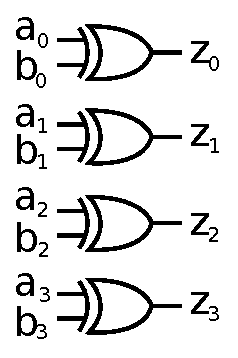
\includegraphics[scale=0.8]{figures/adder4bit.eps}
	\end{center}
	\caption{$4$-bit adder over $\mathbb{F}_{2^4}$.}
	\label{fig:adder4}
\end{figure}
\end{Example}


Conceptually, the multiplication $Z =A\times B \pmod{ P(x) }$ in $\mathbb{F}_{2^k}$ consists of two steps.
In the first step, the multiplication $A\times B$ is performed, and in the second step, the result is reduced
modulo the irreducible polynomial $P(x)$.
Multiplication procedure is shown in Example \ref{exp:mul}.

%\ref{exp1}, 
\begin{Example}
\label{exp:mul}
Consider the field $\mathbb{F}_{2^4}$. We take as inputs:
$A=a_0+a_1\cdot \alpha+a_2\cdot \alpha^2+a_3\cdot \alpha^3$ and
$B=b_0+b_1\cdot \alpha+b_2\cdot \alpha^2+b_3\cdot \alpha^3$, along
with the irreducible polynomial $P(x)=x^4+x^3+1$. We have to perform the
multiplication $Z =A\times B \pmod{ P(x) }$. The coefficients
of $A = \{a_0, \dots, a_3\}, B = \{b_0, \dots, b_3\}$ are in
$\mathbb{F}_2 = \{0, 1\}$. Multiplication can be performed as
shown below:   


{\begin{tabular}{c c c c c c c c}
  &   &   & $a_3$ & $a_2$ & $a_1$ & $a_0$  \\ 
 $\times$&   &   & $b_3$ & $b_2$ & $b_1$ & $b_0$  \\ 
 \hline
 &   &   & $a_3\cdot b_0$ & $a_2 \cdot b_0$ & $a_1\cdot b_0$ & $a_0\cdot b_0$ \\
 &  & $a_3\cdot b_1$ & $a_2\cdot b_1$ & $a_1 \cdot b_1$ & $a_0\cdot b_1$ &   \\
 & $a_3\cdot b_2$ & $a_2\cdot b_2$ & $a_1\cdot b_2$ & $a_0\cdot b_2$ &  &   \\
 $a_3\cdot b_3$ & $a_2\cdot b_3$ & $a_1\cdot b_3$ & $a_0\cdot b_3$ &  &  &   \\
 \hline
 $s_6$& $s_5$  & $s_4$  & $s_3$ & $s_2$  & $s_1$   & $s_0$ 
\end{tabular}}


The result $Sum = s_0+s_1\cdot \alpha + s_2\cdot \alpha^2 + s_3\cdot
\alpha^3 + s_4\cdot \alpha^4 + s_5\cdot \alpha^5 + s_6\cdot \alpha^6$,
\begin{eqnarray}
	s_0  &=&  a_0\cdot b_0 \nonumber \\ 
	s_1  &=&  a_0\cdot b_1 + a_1\cdot b_0 \nonumber \\
	s_2  &=&  a_0\cdot b_2 + a_1\cdot b_1 + a_2\cdot b_0 \nonumber \\
	s_3  &=&  a_0\cdot b_3 + a_1\cdot b_2 + a_2\cdot b_2 +  a_3\cdot b_1\nonumber \\
	s_4  &=&  a_1\cdot  b_3 + a_2\cdot b_1 + a_3\cdot b_1 \nonumber \\
	s_5  &=&  a_2\cdot b_3 + a_3\cdot b_2  \nonumber \\
	s_6  &=&  a_3\cdot b_3   \nonumber
\end{eqnarray}
 Here the multiply ``$\cdot$'' and add ``$+$'' operations are performed
modulo 2, so they can be implemented in a circuit using AND and XOR
gates. Note that unlike integer multipliers, there are no carry-chains
in the design, as the coefficients are always reduced modulo $p =
2$. However, the result is yet to be reduced modulo the primitive
polynomial $P(x) = x^4 + x^3 + 1$. This is shown below, where higher 
degree coefficients are reduced $\pmod{P(x)}$.
% where the final output of the circuit is denoted by $G(x)  = g_3x^3
% + g_2x^2 +g_1x + g_0$.  


{\begin{tabular}{|c c c c | l }
  $s_3$ 	&$s_2$  	&$s_1$   &$s_0$ 	&   \\
 \hline
 $s_4$ 		&$0$		&$0$ 	 &$s_4$  	&$s_4\cdot \alpha^4 \pmod{P(\alpha)} = s_4 \cdot (\alpha^3 + 1)$\\
 $s_5$ 		&$0$		&$s_5$   &$s_5$     &$s_5\cdot \alpha^5 \pmod{P(\alpha)} = s_5\cdot (\alpha^3+ \alpha + 1)$\\
 $s_6$ 		&$s_6$		&$s_6$   &$s_6$     &$s_6\cdot \alpha^6 \pmod{ P(\alpha)} = s_6\cdot( \alpha^3 + \alpha^2 + \alpha + 1)$\\
 \hline
 $z_3$ 		&$z_2$ 		&$z_1$   &$z_0$ 	&
 \end{tabular}\par}


The final result (output) of the circuit is: $Z = z_0 + z_1 \alpha + z_2
\alpha^2 + z_3 \alpha^3$; where  $z_0=s_0+s_4+s_5+s_6; ~~z_1=s_1+s_5+s_6;
~~z_2=s_2+s_6; ~~z_3=s_3+s_4+s_5+s_6$. 
\end{Example}

%%%%%%%%%%%%%%%%%%%%%%%%%%%%%%%%%%%%%%%%%%%%%%%%%%%%%%%%%%%

The above multiplier design is called the {\it Mastrovito multiplier} \cite{mastro:1989} 
which is the most straightforward way to design a multiplier over $\mathbb{F}_{2^k}$. 
A logic circuit for a $4$-bit {\it Mastrovito} multiplier over {\it finite field} $\mathbb{F}_{2^4}$ is illustrated in Fig.\ref{fig:mas4}.

\begin{figure}[b]
	\begin{center}
	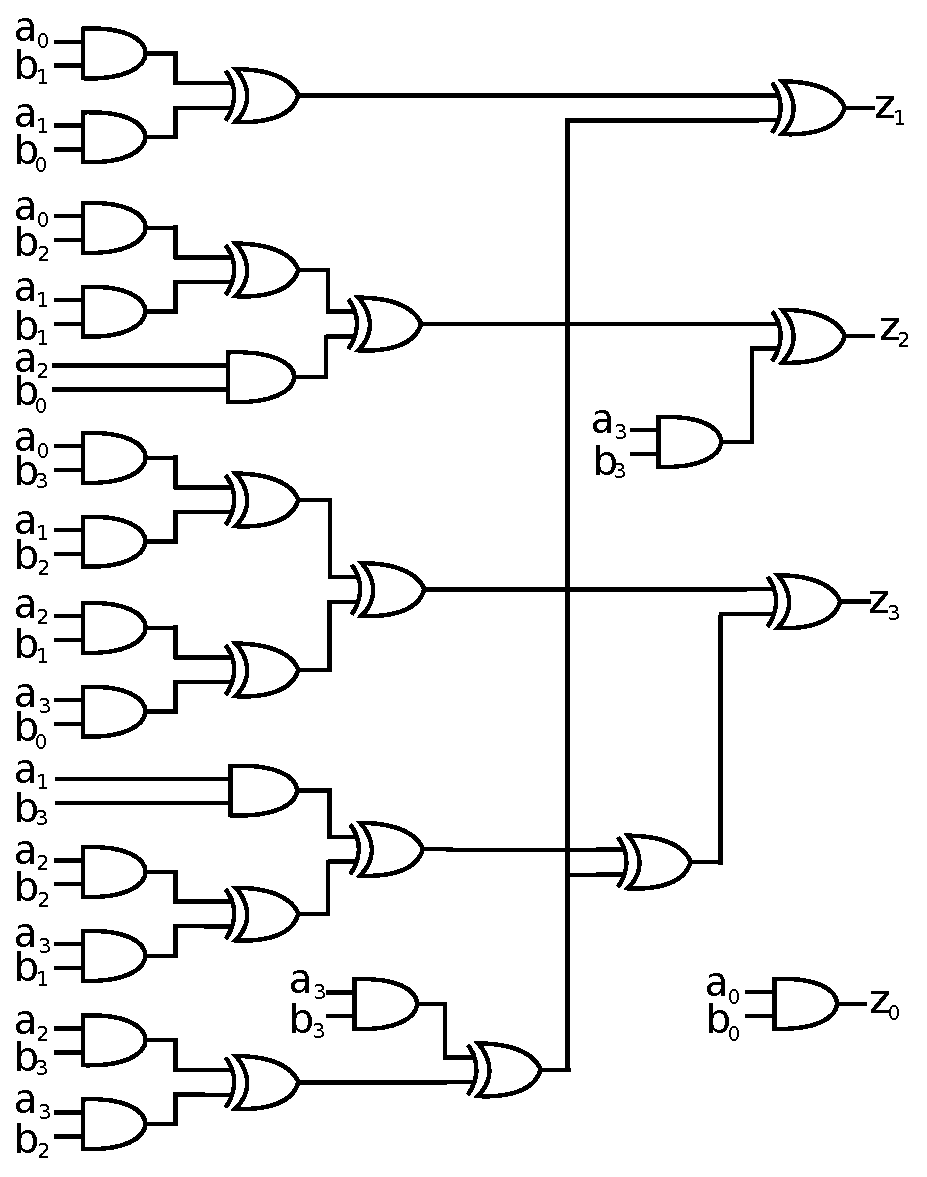
\includegraphics[scale=0.50]{figures/mul4bit.eps}
	\end{center}
	\caption{Mastrovito multiplier over $\mathbb{F}_{2^4}$.}
	\label{fig:mas4}
\end{figure}

Modular multiplication is at the heart of many public-key cryptosystems, 
such as Elliptic Curve Cryptography (ECC) \cite{ecc:1986}. 
Due to the very large field size (and hence the datapath width) used in these cryptosystems, 
the above {\it Mastrovito} multiplier architecture is inefficient, especially when exponentiation and repeat multiplications are performed.
Therefore, efficient hardware and software implementations of modular multiplication algorithms are used to overcome the complexity of such operations. 
These include the Montgomery reduction \cite{PT:1985} \cite{acar:1998} and the Barrett reduction \cite{Knezevic:2008}.

{\bf Montgomery Reduction:}  Montgomery reduction (MR) computes: 

\begin{equation}
G=MR(A,B)=A\cdot B \cdot R^{-1} \pmod {P(x)}
\end{equation}
where $A,B$ are $k$-bit inputs, $R={\alpha}^k$, $R^{-1}$ is multiplicative
inverse of $R$ in $\mathbb{F}_{2^k}$, and $P(x)$ is the irreducible polynomial for
$\mathbb{F}_{2^k}$. Since Montgomery reduction cannot directly compute $A\cdot B$, 
to compute $A\cdot B \pmod {P(x)}$, we need to pre-compute $A\cdot R$ and $B\cdot R$,
as shown in Figure \ref{fig:mm4}.  

\begin{figure}[t]
	\begin{center}
	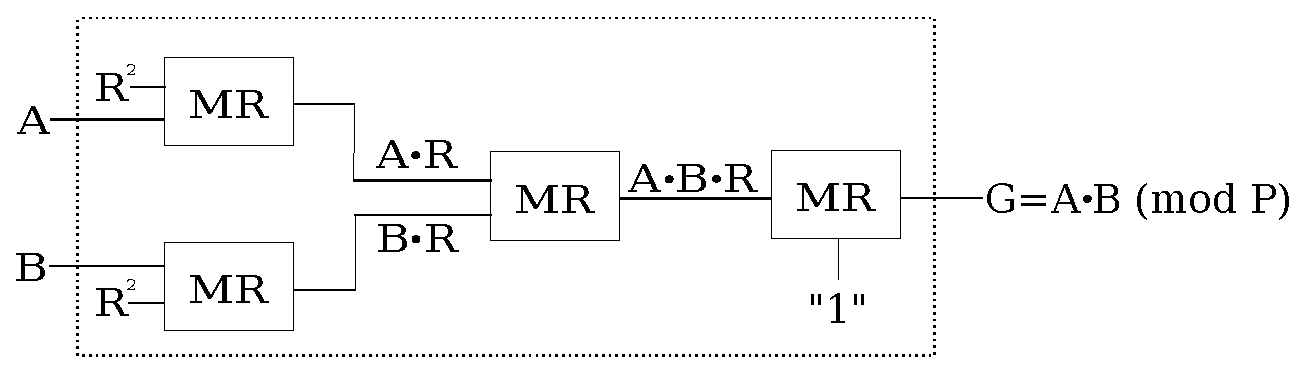
\includegraphics[scale=0.50]{figures/mmcircuit.eps}
	\end{center}
	\caption{{\it Montgomery} multiplier over $\mathbb{F}_{2^k}$}
	\label{fig:mm4}
\end{figure}

Each $\it MR$ block in Figure \ref{fig:mm4} represents a Montgomery reduction step which 
is a hardware implementation of the algorithm shown in Algorithm \ref{alg:mont}. 

\begin{algorithm}
\SetAlgoNoLine

 \KwIn{$A(x), B(x)\in \mathbb{F}_{2^k}$; irreducible polynomial $P(x)$.}
 \KwOut{$G(x)=A(x)\cdot B(x)\cdot x^{-k} \pmod {P(x)}$.}
%%%%%%%%%%%%%%%%%%%%
  $G(x):=$0 \\
  \For { ($i=0$;   $i \le k-1$; ++i ) }
  {
	$G(x):=G(x)+A_i\cdot B(x)$ \CommentSty{/*$A_{i}$ is the $i^{th}$ bit of $A$*/\;}
	$G(x):=G(x)+G_0\cdot P(x)$ \CommentSty{/*$G_{0}$ is the lowest bit of $G$*/\;}
	$G(x):=G(x) / x$ \CommentSty{/*Right shift $1$ bit*/\;}
  }
\caption{Montgomery Reduction Algorithm \cite{acar:1998}}\label{alg:mont}
\end{algorithm}

The design of Fig. \ref{fig:mm4} is an overkill to compute just
$A\cdot B \pmod{ P(x)}$. However, when these multiplications are
performed repeatedly, such as in iterative squaring, then the
Montgomery approach speeds-up the computation. 
As shown in \cite{wu:2002}, the critical path delay and gate counts of a squarer designed using the Montgomery
approach are much smaller than the traditional approaches. 


%For example, here is how to raise y to the th
%%power. I will use “*” to mean “Montgomery-multiply the numbers modulo R”
%\begin{Example}
	
%\end{Example}


{\bf Barrett Reduction:} Barrett reduction is the other widely used multiplier design method adopted in cryptography system designs.
Similar to Montgomery reduction, the traditional Barrett reduction, proposed in \cite{Barrett:1987}, needs a pre-computed value of the reciprocal/inverse of modulus $P(x)$.  
This pre-computation requires extra computational time and memory space. To overcome this limitation, the recent approach of \cite{Knezevic:2008} avoids such a pre-computation of 
inverses and therefore greatly simplifies the hardware design implementation. This algorithmic computation is shown in Algorithm \ref{alg:bar}.

\begin{algorithm}
\SetAlgoNoLine

 \KwIn{$R(x) \in \mathbb{F}_{2^k}$; irreducible polynomial $P(x)=x^n+\displaystyle\sum\limits_{i=0}^l {m_i \cdot x^i}$ satisfying $l=\lfloor \frac{n}{2} \rfloor, m_i \in \{0,1\}$.}
 \KwOut{$G(x)=R(x) \pmod {P(x)}$.}
%%%%%%%%%%%%%%%%%%%%
	$Q_1(x)=\frac{R(x)}{x^n}$ \CommentSty{/*Right shift $n$ bit*/\;}
	$Q_2(x)=P(x) \cdot Q_1(x)$ \;
	$Q_3(x)=\frac{Q_2(x)}{x^n}$ \;
	
	$G_1(x)=R(x) \pmod {x^n}$ \CommentSty{/*Keep the lower $n$ bits of $R(x)$*/\;}
	$G_2(x)=P(x)\cdot Q_3(x) \pmod {x^n}$ \;
	$G(x)=G_1(x) +G_2(x)$ \;
	
\caption{Barrett Reduction Without Pre-Computation Algorithm \cite{Knezevic:2008}}\label{alg:bar}
\end{algorithm}

Based on Barrett reduction, a multiplier can be designed with two simple steps:  multiplication $R=A \times B$ and a subsequent Barrett reduction $G=R \pmod {P}$.
This is shown in Figure \ref{fig:bar}. As we can see, a Barrett multiplier is similar to a Mastrovito multiplier except for the reduction step.

\begin{figure}[hbt]
	\begin{center}
	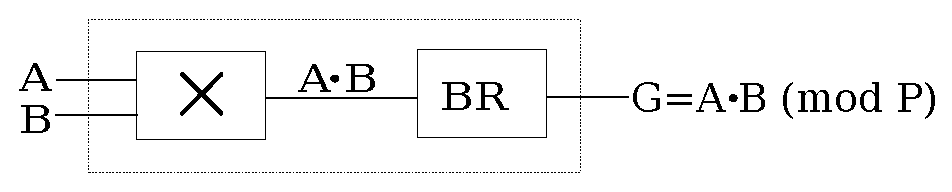
\includegraphics[scale=0.50]{figures/barrett.eps}
	\end{center}
	\caption{Barrett multiplier over $\mathbb{F}_{2^k}$.}
	\label{fig:bar}
\end{figure}

%%%%%%%%%%%%%%%%%%%%%%%%%%%%%%%%%%%%%%%%%%%
One of the most influential applications of finite fields is in elliptic curve cryptography (ECC).
ECC is an approach to public-key cryptography based on the algebraic structure of elliptic curves over finite fields.
%ECC computation is based on an elliptic curve 
The main operations of encryption, decryption and authentication in ECC rely on {\it point multiplications}.
Point multiplication involves a series of addition and doubling of points on the elliptic curve. % -- this, in turn, requires finite field multiplications. 
A drawback of traditional point multiplication is that each point addition and doubling 
involves a multiplicative inverse operation over finite fields.
Representing the points in projective coordinate systems \cite{ecc:software}
eliminates the need for multiplicative inverse operation and therefore increases the efficiency of point multiplication operation.
In our experiments, we have verified custom designs based on L$\acute{o}$pez-Dahab (LD) coordinate system \cite{eccld}. 

\begin{Example}
Consider point addition in LD projective coordinate. Given an elliptic curve: $Y^2 + XYZ = X^3Z + aX^2Z^2 + bZ^4$ over $\mathbb{F}_{2^k}$, 
where $X,Y,Z$ are $k$-bit vectors
that are elements in $\mathbb{F}_{2^k}$ and similarly, $a, b$ are constants from the field. 
Let ($X_1$, $Y_1$, $Z_1$) + ($X_2$, $Y_2$, $1$) = ($X_3$, $Y_3$, $Z_3$) represent point addition over the elliptic curve.
Then $X_3$, $Y_3$, $Z_3$ can be computed as follows:

\begin{align*}
A &= Y_2 \cdot Z_1^2 + Y_1 \\
B &= X_2 \cdot Z_1 + X_1 \\
C &= Z_1 \cdot B \\
D &= B^2 \cdot(C + a Z_1^2) \\
Z_3 &= C^2 \\
E &= A \cdot C  \\
X_3 &= A^2 + D + E  \\
F &= X_3 + X_2 \cdot Z_3 \\
G &= X_3 + Y_2\cdot Z_3 \\
Y_3 &= E\cdot F + Z_3 \cdot G \\
\end{align*}
\end{Example}

\begin{Example}
Consider point doubling in projective coordinate system. Given an elliptic curve: $Y^2 + XYZ = X^3Z + aX^2Z^2 + bZ^4$. 
Let 2($X_1$, $Y_1$, $Z_1$) = ($X_3$, $Y_3$, $Z_3$), then

\begin{align*}
X_3 &= X_1^4 + b \cdot Z_1^4  \\
Z_3 &= X_1^2 \cdot Z_1^2 \\
Y_3 &= b Z_1^4 \cdot Z_3 + X_3 \cdot (aZ_3 + Y_1^2 + bZ_1^4 ) \\
\end{align*}
\end{Example}



In the above examples, polynomoial multiplication and squaring operations are implemented 
in hardware using Montgomery or Barrett reductions over finite fields $\mathbb{F}_{2^k}$. 

The field size for such applications is generally very large; as discussed before, for ECC, in $\mathbb{F}_{2^k}$, $k=163$ or larger.  
Such large size and complicated arithmetic nature of such circuits clearly shows the complexity of the formal verification problem.
Contemporary techniques lack the requisite power of abstraction to model and verify such large systems. 
For this reason,  we propose polynomial abstractions over finite fields to model
and verify such circuits using computer algebra techniques.
This is the subject of subsequent chapters of this dissertation.

%The hardness of such designs lies in the custom-design nature of these circuits. 
%This is because finite fields arithmetic operations are computed modulo $2$, therefore there is no efficient way to describe 
%such arithmetics at high level in hardware description languages, such as {\it Verilog} or {\it VHDL}. 
%In other words, all arithmetic circuits over finite fields $\mathbb{F}_{2^k}$ have to be designed at bit level. 
%In contrast, integer arithmetics can be described easily at word level. For example, as Example \ref{exp:4bitadder}
%shows, a simple {\it Verilog} code $Result[3:0]=A[3:0]+B[3:0]$ is able to express a $4$-bit integer adder. 
%However, a $4$-bit finite field adder cannot be illustrated at word level as $Result[3:0]=A[3:0]+B[3:0]$. 
%Instead, the $4$-bit adder over finite field $\mathbb{F}_{2^4}$ requires to be designed at bit level, as shown in Example \ref{exp:ffadder}.
%Note the modulo $2$ operaton is the same as a $xor$ (\^{}) gate.

%\begin{Example}\label{exp:ffadder}
%\lstset{language=Verilog}
%\begin{lstlisting}
%module Adder(A, B, Result);

   %input [3:0] A;
   %input [3:0] B;
   %output [3:0] Result;

   %assign   Result[0] = A[0] ^ B[0];
   %assign   Result[1] = A[1] ^ B[1] ;
   %assign   Result[2] = A[2] ^ B[2];
   %assign   Result[3] = A[3] ^ B[3];
   
%endmodule
%\end{lstlisting}
%\end{Example}

%Example \ref{exp:ffadder} illustrates the difficulty of designing hardware over finite fields $\mathbb{F}_{2^k}$. 
%Accordingly, the verificaiton of such hardware is also extremely hard.
%This can be attributed to the fact that there is no efficient 
%abstract techniques available for arithmetic circuits over $\mathbb{F}_{2^k}$ 
%while such methods exist for integer arithmetic circuits.
%For example, arithmetic Bit Level (ABL) techniques can be used to abstract integer arithmetic circuits to a higher level and then conduct verification.
%However, such techniques cannot be applied for arithmetic circuits over $\mathbb{F}_{2^k}$.






%%%%%%%%%%%%%%%%%%%%%%%%%%%%%%%%%%%%%%%%%%%%%%%%%%%%%%%%%%%%%%%%%%%%%%%%%%%%
%%%%%%%%%%%%%%%%%%%%%%%%%%%%%%%%%%%%%%%%%%%%%%%%%%%%%%%%%%%%%%%%%%%%%%%%%%%%
%%%%%%%%%%%%%%%%%%%%%%%%%%%%%%%%%%%%%%%%%%%%%%%%%%%%%%%%%%%%%%%%%%%%%%%%%%%%
\chapter{Computer Algebra Fundamentals} \label{ch:ideals}
This chapter reviews preliminary fundamental concepts of commutative and computer algebra that are 
utilized in our work. The concepts of polynomial ideals, varieties and Gr\"obner bases are described with regard to their
algorithmic computation. Finally, the results of Hillbert's Nullstellensatz are described which are employed 
for verification over finite fields in subsequent chapters. The material is mostly referred from 
the textbooks \cite{ideals:book} \cite{gb_book}. 

\section{Monomials and Their Orderings}

\begin{Definition} \label{def:mono}
A {\bf monomial} in $x_1,x_2,\cdots,x_d$ is a product of this form:
\begin{equation}
x_1^{{\alpha}_1} \cdot x_2^{{\alpha}_2} \cdot \cdots x_d^{{\alpha}_d},
\end{equation}
where $\alpha_i \ge 0, i\in\{1,\cdots,d\}$. 
The total degree of the monomial is $\alpha_{1}+\cdots+\alpha_{d}$.
\end{Definition}

For simplicity, we will denote a monomial $x_1^{{\alpha}_1} \cdot x_2^{{\alpha}_2} \cdot \cdots x_d^{{\alpha}_d}=x^{\alpha}$, 
where $\alpha=({\alpha}_1,\cdots,{\alpha}_d)$, i.e., $\alpha \in \mathbb{Z}_{\ge 0}^{d}$.
  
%From Definition \ref{def:poly}, we know a polynomial can be expressed as:
%\begin{equation} \label{eq:poly1}
%f= \sum_i a_i x^i = a_0 + a_1 x + a_2 x^2 + \cdots + a_d x^d, a_i \in k;
%\end{equation}

\begin{Definition}
A {\bf multivariate polynomial} $f$ in variables $x_1, x_2, \ldots, x_d$ with coefficients in any 
given field $\mathbb{K}$ is a finite linear combination (with coefficients in $\mathbb{K}$) of monomials:
\begin{equation}
	f=\sum_{\alpha}a_{\alpha}\cdot x^{\alpha}, ~~a_{\alpha}\in \mathbb{K} \nonumber
\end{equation}
\end{Definition}

The set of all polynomials in $x_1, x_2, \ldots, x_d$ with coefficients in field $\mathbb{K}$ 
is denoted by $\mathbb{K}[x_1, x_2, \ldots, x_d]$.

%$\mathbb{R}[x]$ is the set of polynomials in $x$ with coefficients in $\mathbb{R}$, so $2x^3+\frac{7}{4}x \in \mathbb{R}[x]$. 
%$\mathbb{Z}_p[x,y]$ is the set of polynomials in $x,y$ with coefficients in $\mathbb{Z}_p$, where $p$ is a prime number. 
%$\mathbb{F}_{2^k}[x_0,x_1, x_2, \ldots, x_d]$ is the set of polynomials in $x_0,x_1, x_2, \ldots, x_d$ with coefficients in $\mathbb{F}_{2^k}$, where $k>0$.

\begin{Definition}
Let $f=\sum_{\alpha} a_{\alpha} x^{\alpha}$ be a polynomial in $\mathbb{K}[x_1, x_2, \ldots, x_d]$. 
\begin{enumerate}
\item We refer to the constant $a_{\alpha} \in \mathbb{K}$ as the \textit{coefficient} of the monomial $a_{\alpha} x^{\alpha}$.
\item If $a_{\alpha} \neq 0$, we call $a_{\alpha} x^{\alpha}$ a term of $f$.
\end{enumerate}
\end{Definition}

As an example, $2x^2+y$ is a polynomial with two terms $2x^2$ and $y$, with $2$ and $1$ as coefficients respectively. 
In contrast, $x+y^{-1}$ is not a polynomial because the exponent of $y$ is less than $0$.

An important fact of polynomials is that a polynomial is a sum of terms and 
these terms have to be arranged unambiguously so that they can be manipulated in a consistent manner.
Therefore, we need establish the concept {\bf monomial ordering (or term ordering)}.
A term ordering, represented by $>$, defines how
terms in a polynomial are ordered.  Term-orderings are totally ordered,
i.e. anti-symmetric, transitive, total, with constant terms last in the ordering. 
More formally, we have the following definitions:
%%%%%%%%%%%%%%%%%%%   monomial    Ordering   %%%%%%%%%%%%%%%%%%%%%%%%%%%%
\begin{Definition}
Let $\mathbb{T}^{d}=\{x^{\alpha}: \alpha\in \mathbb{Z}_{\ge 0}^{d}\}$ be the set of all monomials in $x_{1},\dots,x_{d}$.
A {\bf monomial order} $>$ on $\mathbb{T}^{d}$ is a total well-ordering satisfying:
\begin{itemize}
	\item For any $x^{\alpha} \in \mathbb{T}^{d}$, $x^{\alpha}>1$
	\item For all $\alpha, \beta, \gamma$, $x^{\alpha}>x^{\beta} \Rightarrow x^{\alpha} \cdot x^{\gamma}> x^{\beta} \cdot x^{\gamma}$
\end{itemize}
\end{Definition}

A total-order ensures that there is no ambiguity with respect to where a term is found in 
the term-ordering.  Total orderings for monomials come in different forms, notably 
{\bf lexicographic orderings} (lex), and its variants: {\bf degree-lexicographic ordering} (deglex) 
and {\bf reverse degree-lexicographic ordering} (revdeglex).

A {\bf lexicographic ordering} (lex) is a total-ordering $>$ such that variables
in the terms are lexicographically ordered.  Higher variable-degrees take 
precedence over lower degrees (e.g. $a^3 = a a a$).
\begin{Definition}
{\bf Lexicographic order:} Let $x_1 > x_2 > \dots > x_d$
lexicographically. Also let $\alpha = (\alpha_1, \dots, \alpha_d);
~\beta = (\beta_1, \dots, \beta_d) \in \mathbb{Z}^d_{\geq 0}$. Then we
have: 
\begin{equation}
x^{\alpha} > x^{\beta} \iff 
\begin{cases}
& \text{Starting  from the  left, the first co-ordinates of $\alpha_i, \beta_i$} \\
& \text{that are different satisfy $\alpha_i > \beta_i$}

\end{cases}
\end{equation}
\end{Definition}

A {\bf degree-lexicographic ordering} (deglex) is a total-ordering $>$ such that 
the total degree of a term takes precedence over the lexicographic ordering.  A
{\bf degree-reverse-lexicographic ordering} (degrevlex) is the same as a
deglex ordering, however terms are lexed in reverse.

\begin{Definition}
{\bf Degree Lexicographic order:} Let $x_1 > x_2 > \dots > x_d$
lexicographically. Also let $\alpha = (\alpha_1, \dots, \alpha_d);
~\beta = (\beta_1, \dots, \beta_d) \in \mathbb{Z}^d_{\geq 0}$. Then we
have: 
\begin{equation}
x^{\alpha} > x^{\beta} \iff 
\begin{cases}
\sum_{i=1}^{d}\alpha_i > \sum_{i=1}^{d} \beta_i & \text{ or }\\
\sum_{i=1}^{d}\alpha_i = \sum_{i=1}^{d} \beta_i  \text{ and }
x^{\alpha} > x^{\beta} & \text{w.r.t. lex order}
\end{cases}
\end{equation}
\end{Definition}


\begin{Definition}
{\bf Degree Reverse Lexicographic order:} Let $x_1 > x_2 > \dots > x_d$
lexicographically. Also let $\alpha = (\alpha_1, \dots, \alpha_d);
~\beta = (\beta_1, \dots, \beta_d) \in \mathbb{Z}^d_{\geq 0}$. Then we
have: 
\begin{equation}
x^{\alpha} > x^{\beta} \iff 
\begin{cases}
\sum_{i=1}^{d}\alpha_i > \sum_{i=1}^{d} \beta_i  \text{ or }\\
\sum_{i=1}^{d}\alpha_i = \sum_{i=1}^{d} \beta_i  \text{ and the first co-ordinates}\\
\text{$\alpha_i, \beta_i$ from the right, which are different, satisfy $\alpha_i < \beta_i$}
\end{cases}
\end{equation}

\end{Definition}

As a consequence of these term orderings, we have the following relations, where $a > b > c$.

\begin{eqnarray}
    \eqntext{lex:}  
    a^2b > a^2 > abc > ab > ac^2 > ac > b^2c > b^2 > bc^3 > 1 
    \label{ex:ordering:lex}\\
    \eqntext{deglex:} 
    bc^3 > a^2b > abc > ac^2 > b^2c > a^2 > ab >
    ac > b^2 > 1
    \label{ex:ordering:deglex}\\
    \eqntext{degrevlex:}  
    bc^3 > a^2b > abc > b^2c > ac^2 > a^2 > ab >
    b^2 > ac > 1
    \label{ex:ordering:degrevlex}
\end{eqnarray}

The difference between the {\it lex} and two {\it deg-} orderings is
obvious, while the difference between the two degree-based orderings can be
seen by considering from which direction the term is lexed, e.g. $ac^2 > b^2c$ (deglex, left-to-right)
versus $b^2c > ac^2$ (degrevlex, right-to-left). 

\begin{Example}
Let $f = 2x^2yz + 3xy^3 - 2x^3$. Effects of different term orderings on $f$ are shown below:
\begin{itemize}
\item lex $x> y> z$: $f = -2x^3 + 2x^2yz + 3xy^3$
\item deglex $x>y>z$:  $f = 2x^2yz + 3xy^3 -2x^3$
\item degrevlex $x>y>z$: $f = 3xy^3 + 2x^2yz - 2x^3$
\end{itemize}
\end{Example}

%Based on the {\it monomial ordering}, we have the following concepts:

\begin{Definition}
The {\bf leading term} is the first term in a term-ordered polynomial.
Likewise, the {\it leading coefficient} is the coefficient of
the leading term.  Finally, a {\it leading power product} is the leading term 
lacking the coefficient.  We use the following notation:
\begin{eqnarray}
     lt(f)&& \text{--- Leading Term} \\
     lc(f)&& \text{--- Leading Coefficient} \\
     lm(f)&& \text{--- Leading Monomial}
\end{eqnarray}
\end{Definition}

\begin{Example}
\begin{eqnarray}
     f      &=& 3a^2b + 2ab + 4bc \\
     lt(f)  &=& 3a^2b \\
     lc(f)  &=& 3 \\
     lm(f)  &=& a^2b
\end{eqnarray}
\end{Example}

\section{Varieties and Ideals}
%%%%%%%%%%%%%%%%%%%%%%%%%%%%%%%%%%%%%%%%%%%%%%%%%%%%%%%%%%%%%%%%%%%%%%%%%%%%
%%%%%%%%%%%%%%%%%%%%%  variety %%%%%%%%%%%%%%%%%%%%%%%%%%%%%%%%%%%%%%%%%%
In verification applications, it is often required to analyze (the presence or absence of) solutions to a given system of constraints.
In our applications, these constraints are polynomials and their solutions are described as {\bf varieties}.

\begin{Definition}
Let $\mathbb{K}$ be a field, and let $f_1, \ldots, f_s \in \mathbb{K}[x_1, x_2, 
\ldots, x_d]$. We call $V(f_1, \dots, f_s)$ the {\bf affine variety} defined by $f_1, \dots, f_s$ as:
\begin{equation}
V(f_1, \ldots, f_s)= \{(a_1, \ldots, a_{d})\in \mathbb{K}^d:f_i(a_1, \ldots, a_d)=0, \forall{i},1\le i \le s\}.
\end{equation}
\end{Definition}

$V(f_1, \dots, f_s)\in \mathbb{K}^d$ is {\bf the set of  all solutions} of the system of equations: 
$f_1(x_1,\ldots,x_d)=\dots=f_s(x_1,\dots,x_d)=0$. 

\begin{Example}
Given $\mathbb{R}\left[x,y\right]$, $V(x^2+y^2)=\{(0,0)\}$. 
Similarly, in $\mathbb{R}\left[x,y\right]$, $V(x^2+y^2-1)=\{all\  points\  on\ the\ circle: x^2+y^2-1=0\}$.
However, varieties depend on which field we are operating on. For the same polynomial $x^2+1$, we have:
\begin{itemize}
\item In $\mathbb{R}[x]$, $V(x^2+1)=\emptyset$.
\item In $\mathbb{C}[x]$, $V(x^2+1)=\{(\pm i)\}$.
\end{itemize}
\end{Example}

The above example shows the variety can be infinite, finite (non-empty set) or empty.
It is interesting to note that we will be operating over finite fields $\mathbb{F}_{q}$, 
and any finite set of points is a variety.  
Consider the points $\{(a_1,\dots, a_d): a_1, \dots, a_d \in \mathbb{F}_q\}$
in $\mathbb{F}_q^d$. Any single point is a variety of some polynomial system:
e.g. $(a_1,\dots, a_d)$ is a variety of $x_1-a_1 = x_2 - a_2 = \dots =
x_d-a_d=0$. Moreover, {\bf finite unions and finite  intersections} of
varieties are also varieties. Let $U = V(f_1, \dots, f_s)$ and $W =
V(g_1, \dots, g_t)$. Then:  
\begin{itemize}
\item $U \cap W = V(f_1, \dots, f_s, g_1, \dots, g_t)$
\item $U \cup W = V(f_i g_j: 1 \leq i \leq s, 1 \leq j \leq t)$
\end{itemize}

Another important concept related to varieties is that the variety depends not just on the given system of polynomial equations,but
rather on the {\bf ideal} generated by the polynomials.

%%%%%%%%%%%%%%%%%%%%%  ideal %%%%%%%%%%%%%%%%%%%%%%%%%%%%%%%%%%%%%%%%%%
\begin{Definition} 
A subset $I \subset \mathbb{K}[x_1, x_2, \ldots, x_d]$ is an {\bf ideal} if it satisfies:
\begin{itemize}
\item $0 \in I$
\item $I$ is closed under addition: $x, y \in I \Rightarrow x+y \in I$
\item If $x \in \mathbb{K}[x_1, x_2, \ldots, x_d]$ and $y \in I$, then $x\cdot y \in I$ as well as $y\cdot x \in  I$.
\end{itemize}
\end{Definition}

Any ideal is generated by its {\it basis} or {\it generators}.

%%%%%%%%%%%%%%%%%%%%%  ideal basis%%%%%%%%%%%%%%%%%%%%%%%%%%%%%%%%%%
\begin{Definition}
Let $f_1, f_2, \ldots, f_s$ be the given elements of $\mathbb{K}[x_1, x_2, \ldots, x_d]$. 
Let $I$ be an ideal in $\mathbb{K}[x_1, x_2, \ldots, x_d]$. If:
\begin{equation}
I = \{g_1 f_1 + g_2 f_2 + \ldots + g_s f_s: g_1, \ldots, g_s \in \mathbb{K}[x_1, x_2, \ldots, x_d]\}
\end{equation}
then, $f_1, \ldots, f_s$ are called the {\bf basis (or generators)} of the ideal $I$ and 
correspondingly $I$ is denoted as $I = \langle f_1, f_2, \ldots, f_s \rangle$. 
\end{Definition}


\begin{Example}
The set of even integers, which is a subset of the ring of integers
$Z$, forms an ideal of $Z$. This can be seen from the following;
\begin{itemize}
\item $0$ belongs to the set of even integers.
\item The sum of two even integers $x$ and $y$ is always an even
  integer.
\item The product of any integer $x$ with an even integer $y$ is
  always an even integer.
\end{itemize}
\end{Example}

\begin{Example}
Given $\mathbb{R}\left[x,y\right]$, $I = \langle x, y \rangle$ is an 
ideal containing all polynomials generated by $x$ and $y$, such as $x^2+y$, $x\cdot y+x$. 
$J = \langle x^2, y^2 \rangle$ is an ideal containing all polynomials generated by $x^2$ and $y^2$, 
such as $x^2+y^2$, $x^2\cdot y^2+x^{10}$. Notice $I\neq J$ because $x+y$ can only be generated by $I$.
\end{Example}


Any ideal may have many different bases. For instance, it is possible to have different sets of polynomials
$\{f_1,\dots,f_{s}\}$ and $\{g_{1},\dots,g_{t}\}$ that may generate the same ideal, i.e., 
$\langle f_{1},\dots,f_{s}\rangle=\langle g_{1},\dots,g_{t}\rangle$. Since variety depends on the ideal, 
these sets of polynomials have the same solutions.

\begin{Proposition}
	If $f_1,\dots,f_{s}$ and $g_{1},\dots,g_{t}$ are bases of the same ideal in $\mathbb{K}[x_{1},\dots,x_{d}]$,
	so that $\langle f_{1},\dots,f_{s}\rangle=\langle g_{1},\dots,g_{t}\rangle$, then 
	$V(f_{1},\dots,f_{s})=V(g_{1},\dots,g_{t})$.
\end{Proposition}

\begin{Example}
	Consider the two bases $F_{1}=\{(2x^{2}+3y^{2}-11,x^{2}-y^{2}-3\}$ and $F_{2}=\{x^{2}-4,y^{2}-1\}$.
	These two bases generate the same ideal, i.e., $\langle F_{1}\rangle= \langle F_{2} \rangle$.{}
	Therefore, they represent the same variety, i.e., 
	\begin{equation}
		V(F_{1})= V( F_{2})=\{\pm 2, \pm 1\}.
	\end{equation}
\end{Example}

An important fundamental problem that we need to solve is one of ideal membership testing.
\begin{Definition}
	Let $f, f_{1},\dots, f_{s}$ be polynomials in $\mathbb{K}[x_{1},\dots,x_{d}]$.
	Let ideal $I=\langle f_{1},\dots, f_{s} \rangle \subset \mathbb{K}[x_{1},\dots,x_{d}]$.
	If $f$ can be written as $f=f_{1}h_{1}+\dots+f_{s}h_{s}$, then we say $f$ is a member of the ideal $I$. 
\end{Definition}

Our verification problems are formulated as ideal membership testing. For this purpose, we require a decision procedure
to unequivocally decide ideal membership. Gr\"obner basis provides such a decision procedure, and this is described in 
the next section. 

%%%%%%%%%%%%%%%%%%%%	Grobner bases	%%%%%%%%%%%%%%%%%%%%%%%%%%%%%%%%%%
\section{Gr\"obner Bases}

As mentioned above, different generating sets may constitute the same ideal. However, some generating sets
may be better than others -- that is they may be a better representation of the ideal. A {\bf Gr\"obner basis}
is one such ideal representation that has many important properties that allow to solve many polynomial decision
questions. By analyzing the Gr\"obner basis, one can deduce the presence or absence of solutions (varieties), 
find the dimension of the varieties, and also deduce ideal membership. 
A Gr\"obner basis, in essence, is a canonical representation of an ideal.
Buchberger's work \cite{buchberger_thesis} laid the
foundation for computing a Gr\"obner basis of an ideal.  
This section provides a synopsis of some of these concepts.

%The theory of Gr\"obner's bases provides an algorithmic
%framework to determine a better generating set for any ideal. 

Among many equivalent definitions of Gr\"obner bases, we start with the definition that can best describe the 
properties of Gr\"obner bases:

\begin{Definition}
    A set of non-zero polynomials
    $G=\{g_1,\dots,g_t\}$ contained in an ideal $I$, is called a {\bf Gr\"obner
    basis} for $I$ if and only if for all $f \in I$ such that $f \neq 0$,
    there exists $i \in \{1,\dots,t\}$ such that $lm(g_i)$ divides $lm(f)$.
    \begin{eqnarray}
        G = \text{Gr\"obner{Basis}} (I) \iff \forall f \in I: f \neq 0, \exists
        g_i \in G: lm(g_i)\ |\ lm(f)
        \label{eqn:groebnermin}
    \end{eqnarray}
    
\end{Definition}

Given a set of polynomials $F=\{f_{1},\dots,f_{s}\}$ that generate ideal $I=\langle f_{1},\dots,f_{s} \rangle$, 
Buchberger gives an algorithm to compute a Gr\"obner basis $G=\langle g_{1},\dots,g_{t}\rangle$. This algorithm relies on 
the notions of $S$-polynomials and polynomial reduction, which are described below.

%Little can be understood about a Gr\"obner basis without understanding
%how the basis is derived.  To derive a Gr\"obner basis, some additional definitions are necessary:

%\begin{Definition}
    %The {\bf least common multiple} of a pair of numbers $f$ and $g$,
    %denoted $lcm(f,g)$, is the smallest number, greater than zero,  which is 
    %a multiple of both.
%\end{Definition}

%For example:
%\begin{eqnarray*}
    %lcm(3,4) = 12 \\
    %lcm(6,8) = 24 
%\end{eqnarray*}

\begin{Definition}
    For a field $\mathbb{K}, f, g \in \mathbb{K}[x_1,\dots,x_d], L = lcm\left(lt(f), lt(g)\right)$,
    an {\bf S-polynomial} $Spoly(f,g)$ is defined as:
    \begin{equation}
        Spoly(f,g)=\frac{L}{lt(f)}\cdot f - \frac{L}{lt(g)}\cdot g
        \label{eqn:spoly}
    \end{equation}
Note $lcm$ denotes least common multiple. 
\end{Definition}

\begin{Definition}
    The {\bf reduction} of a polynomial $f$, by another polynomial $g$, to
    a reduced polynomial $r$ is denoted:
    \begin{equation*}
        f\stackrel{g}{\textstyle\longrightarrow}r
    \end{equation*}
    Reduction is carried out using multivariate, polynomial long division. 
    % The long division is performed according to a term-ordering on polynomials, and the division algorithm 
    %terminates when the leading term of the divisor does not divide any 
    %other term in the dividend.
  
    For sets of polynomials, the notation 
    \begin{equation*}
    f\stackrel{F}{\textstyle\longrightarrow}_+r    
    \end{equation*}
    represents the reduced polynomial $r$ resulting from $f$ as reduced by a 
    set of non-zero polynomials $F = \{f_1,\dots,f_s\}$.  The polynomial $r$ is considered {\bf reduced} if 
    $r = 0$  or no term in $r$ is divisible  by a $lm(f_i), \forall f_i \in F$.
\end{Definition}

  For all intents and purposes, the reduction process
    $f\stackrel{F}{\textstyle\longrightarrow}_+r$, of dividing a 
    polynomial $f$ by a set of polynomials of $F$, can be modeled as
    repeated long-division of $f$ by each of the polynomials in $F$ until no
    further reductions can be made---the result of which is $r$, as shown in Algorithm \ref{alg:polydiv}.

\begin{algorithm}[hbt]
\SetAlgoNoLine

 \KwIn{$f,f_{1},\dots,f_{s}$}
 \KwOut{$r,a_{1},\dots,a_{s}$, such that $f=a_{1}\cdot f_{1}+\dots+a_{s}\cdot f_{s}+r$.}
 
 $a_{1}=a_{2}=\dots=a_{s}=0$; $r=0$\;
 $p:=f$\;
 
 \While { $p \neq 0$ }
 {
	i=1\;
	divisionmark = false\;
	\While { $i\le s  $ \&\& divisionmark = false }
	{
		\eIf {$f_{i}$ can divide $p$}
		{
			$a_{i}=a_{i}+lt(p)/lt(f_{i})$\;
			$p=p-lt(p)/lt(f_{i}) \cdot f_{i}$\;
			divisionmark = true\;
		}
		{
			i=i+1\;
		}
	}
	
	\If {divisionmark = false}
	{
		$r=r+lt(p)$\;
		$p=p-lt(p)$\;
	}

 }
\caption{Polynomial Division}\label{alg:polydiv}
\end{algorithm}

The division algorithm keeps cancelling the leading terms of polynomials until no more leading terms can be further cancelled.
So the key step is $p=p-lt(p)/lt(f_{i}) \cdot f_{i}$, as the following example shows.
\begin{Example}
	Given $f_{1} = y^{2}-x$ and $f_{2} = y - x$ in $\mathbb{Q}[x,y]$ with $deglex$: $y>x$. 
Then $f_{1}/f_{2}=f_{1}-lt(f_{1})/lt(f_{2}) \cdot f_{2}=y^{2}-x-(y^{2} /y) \cdot (y-x)=y\cdot x-x$.
Then $y\cdot x-x$ can be further divided by $f_{2}$: $(y\cdot x-x)/f_{2}=x^{2}-x$ which is the final result.
\end{Example}

We now present Buchberger's Algorithm \cite{buchberger_thesis} for computing Gr\"obner
bases. 

\begin{algorithm}[hbt]
\SetAlgoNoLine
 \KwIn{$F = \{f_1, \dots, f_s\}$, such that $I=\langle f_1, \dots, f_s\rangle$}
 \KwOut{$G = \{g_1,\dots ,g_t\}$, a Gr\"{o}bner basis of $I$ }
  $G:= F$\;
  \Repeat{$G = G'$}
  {
  	$G' := G$\;
  	\For{ each pair $\{f_{i}, f_{j}\}, i \neq j$ in $G'$} 
	{
		$Spoly(f_{i}, f_{j}) \stackrel{G'}{\textstyle\longrightarrow}_+r$ \;
		\If{$r \neq 0$}
		{
			$G:= G \cup \{r\}$ \;
		}
	}
   }
\caption {Buchberger's Algorithm}\label{alg:gb}
\end{algorithm}


For Gr\"obner basis computation, a monomial (term) ordering is
fixed to ensure that polynomials are manipulated in a consistent manner. 
Buchberger's algorithm then takes pairs of polynomials ($f_{i}, f_{j}$) in the basis $G$
and combines them into ``$S$-polynomials'' (Spoly($f_{i}, f_{j}$)) to cancel leading terms. The
$S$-polynomial is then reduced (divided) by all elements of $G$ to a
remainder $r$, denoted as  $S(f_{i}, f_{j}) \stackrel{G}{\textstyle\longrightarrow}_+r$. 
Multivariate polynomial division is used for this reduction step. This
process is repeated for all unique pairs of polynomials, including
those created by newly added elements, until no new polynomials are
generated; ultimately constructing the Gr\"{o}bner basis.

\begin{Example}\label{exp:gbsimple}
Consider the ideal $I \subset \mathbb{Q}[x, y]$, $I = \langle f_1, f_2 \rangle$,
where $f_1 = yx - y, ~f_2 = y^2 - x$. Assume a degree-lexicographic term ordering with $y > x$ is imposed. 

First, we need to compute $Spoly(f_{1},f_{2})=x\cdot f_{2}-y\cdot f_{1}=y^{2}-x^{2}$.
Then we conduct a polynomial reduction 
$y^{2}-x^{2}\stackrel{f_{2}}{\textstyle\longrightarrow}x^{2}-x \stackrel{f_{1}}{\textstyle\longrightarrow}x^{2}-x$.
Let $f_{3}=x^{2}-x$. Then $G$ is updated as $\{f_{1},f_{2},f_{3}\}$. Next we compute $Spoly(f_{1},f_{3})=0$. So there
is no new polynomial generated. Similarly, we compute $Spoly(f_{2},f_{3})=x\cdot y^{2}-x^{3}$, followed by 
$x\cdot y^{2}-x^{3}\stackrel{f_{1}}{\textstyle\longrightarrow}y^{2}-x^{3} \stackrel{f_{2}}{\textstyle\longrightarrow}x-x^{3}
\stackrel{f_{2}}{\textstyle\longrightarrow}0$. Again, no polynomial is generated. Finally, $G=\{f_{1,}f_{2},f_{3}\}$.

\end{Example}


Gr\"obner basis now gives a decision procedure to test for membership in an ideal.

%With the knowledge of Gr\"obner basis and polynomial reduction procedure,  we get the following {\bf ideal
%membership testing} algorithm: given an ideal $I =\langle f_1, \cdots,f_s \rangle$, we can decide whether a
%given polynomial $f$ is a member of the ideal $I$. 
%First, we compute a Gr\"obner basis $G = {g_1,\cdots,g_t }$ using Algorithm \ref{alg:gb}.

    
\begin{Theorem}\label{the:membership}
	Let $G = \{g_1,\cdots,g_t \}$ be a Gr\"obner basis for an ideal $I \subset \mathbb{K}[x_1,\cdots,x_d ]$
	and let $f \in \mathbb{K}[x_{1},\dots, x_{d}]$. Then $f \in I$ if and only if the remainder on division of $f$ by
	$G$ is zero.
\end{Theorem}
In other words, 
\begin{equation}
f \in I \iff f \stackrel{G}{\textstyle\longrightarrow}_+0
\end{equation}



\begin{Example}
Consider Example \ref{exp:gbsimple}. Let $f = y^2x - x$ be another
polynomial. Note that $f = yf_1 + f_2$, so $f \in I$. If we divide $f$
by $f_1$ first and then by $f_2$, we will obtain a zero
remainder. However, since the set $\{f_1, f_2\}$ is not a Gr\"{o}bner
basis, we find that the reduction $f
\stackrel{f_2}{\textstyle\longrightarrow} x^2 - x
\stackrel{f_1}{\textstyle\longrightarrow} x^2 - x  \neq 0$;
i.e. dividing $f$ by $f_2$ first and then by $f_1$ does not lead to a
zero remainder. However,  if we compute the Gr\"{o}bner basis $G$ of
$I$, $G = \{x^2 - x, yx - y, y^2 - x\}$, dividing $f$ by polynomials
in $G$ in any order will always lead to the zero remainder. Therefore,
one can decide ideal membership unequivocally using the Gr\"{o}bner
basis. 
\end{Example}

\begin{Definition}\label{def:minigb}
A {\bf minimal Gr\"obner basis} for a polynomial ideal $I$ is a Groebner basis $G$ for $I$ such that
	\begin{itemize}
		\item $lc(g_{i})=1,\forall g_{i}\in G$
		\item $\forall g_{i} \in G$,  $lt(g_{i}) \notin \langle lt(G-\{g_{i}\})\rangle$
	\end{itemize}
\end{Definition}
A {\bf minimal} Gr\"obner basis is a Gr\"obner basis such that 
no leading term of any element in $G$ divides another in $G$.
A  minimal Gr\"obner basis can be computed by removing 
any polynomial whose leading term can be divided by another in a given Gr\"obner basis.
    
A minimal Gr\"obner basis can be further reduced.
\begin{Definition}
	A {reduced Gr\"obner basis} for a polynomial ideal $I$ is a Gr\"obner basis $G=\{g_{1},\dots,g_{t}\}$ such that:
	\begin{itemize}
		\item $lc(g_{i})=1,\forall g_{i}\in G$
		\item $\forall g_{i} \in G$, no monomial of $g_{i}$ lies in $\langle lt(G-\{g_{i}\})\rangle$
	\end{itemize}
\end{Definition}
$G$ is a reduced Gr\"obner basis when no monomial of any element in $G$ divides the leading term of another element.

For a given monomial ordering, 
the reduced Gr\"obner basis is a canonical representation of the ideal, as given by Proposition \ref{pro:unique} below.


\begin{Proposition}\label{pro:unique}
Let $I \neq \{0\}$ be a polynomial ideal. Then, for a given monomial ordering, $I$ has a unique reduced Gr\"obner basis.
\end{Proposition}

%%%%%%%%%%%%%%%%%%%%%%%%%%%%%%%%%%%%%%%%%%%%%
%%%%%%%%%%%%%%%%%%%%%%%%%%%%%%%%%%%%%%%%%%%%%
\section{Hillbert's Nullstellensatz}

In this section, we further describe some correspondence between ideals and varieties in
the context of algebraic geometry. The celebrated results of Hillbert's Nullstellensatz
establish such correspondences, and these results, together with Gr\"obner bases, 
provide a basis for our verification solutions. 

%%%%%%%%%%%%%%%%%algebraically closed field%%%%%%%%%%%%%
\begin{Definition}\label{def:acf}
A field $\overline {\mathbb{K}}$ is an algebraically closed field if every polynomial in one variable with degree at least $1$, with coefficients 
in $\overline {\mathbb{K}}$, has a root in $\overline {\mathbb{K}}$.
\end{Definition}
In other words, any non-constant polynomial equation over $\overline {\mathbb{K}}\left[x\right]$ always has at least one root 
in $\overline {\mathbb{K}}$. Every field $\mathbb{K}$ is contained in an algebraically closed one $\overline {\mathbb{K}}$. 
For example, the field of reals $\mathbb{R}$ is not an algebraically closed field, because $x^2+1=0$ 
has no root in $\mathbb{R}$. However, $x^2+1=0$ has roots in the field of complex numbers $\mathbb{C}$, 
which is an algebraically closed field. 
In fact, $\mathbb{C}$ is the algebra closure of $\mathbb{R}$.
Every algebraically closed field is an infinite field.

%%%%%%%%%%%%%%%%weak nullstellensatz%%%%%%%%%%%%%
\begin{Theorem}
$\left[\bf{Weak\  Nullstellensatz}\right]$ Let $I \subset \overline {\mathbb{K}}[x_1, x_2, \cdots, x_d]$ be an ideal satisfying $V(I)=\emptyset$. 
Then $I=\overline {\mathbb{K}}[x_1, x_2, \cdots, x_d]$, Or equivalently, 
\begin{equation}
V(I)=\emptyset\ \iff\ I=\overline {\mathbb{K}}[x_1, x_2, \cdots, x_d]=\langle 1 \rangle 
\end{equation}
\end{Theorem}

\begin{Corollary}
	Let $I=\langle f_{1},\dots,f_{s} \rangle \subset \overline {\mathbb{K}}[x_1, x_2, \cdots, x_d]$. 
	Let $G$ be the reduced Gr\"obner basis of $I$. Then $V(I)=0 \iff G=\{1\}$.
\end{Corollary}

The {\it Weak Nullstellensatz} offers a way to evaluate whether or not the system of multivariate polynomial equations (ideal $I$) has common solutions 
in ${\overline {\mathbb{K}}}^d$. For this purpose, we only need to check if the ideal is generated by the unit element, i.e., $1\in I$. 
This approach can be used to evaluate the feasibility of constraints in our verification problems. 
Another interesting result that we will employ is one of {\bf Strong Nullstellensatz} to describe which we need the concepts of ``ideals of varieties" and 
radicals.
%%%%%%%%%%%%%%%%%%%%%%%%%%%%strong Nullstellensatz%%%%%%%%%%%%%%%%%%%%%%%%%%%%%%

Let $\mathbb{K}$ be any field and let $\mathbf{a}=(a_{1},\dots,a_{d}) \in \mathbb{K}^d$ be a point, and $f \in
\mathbb{K}[x_1,\dots, x_d]$ be a polynomial. We say that $f$ {\it vanishes} on $\mathbf{a}$ if $f(\mathbf{a}) = 0$, i.e.,
$\mathbf{a}$ is in the variety of $f$.

\begin{Definition}
For any variety $V$ of $\mathbb{K}^d$, the ideal of polynomials that vanish on $V$,
called the {\it vanishing ideal of $V$}, is defined as $I(V) = \{f\in
\mathbb{F}[x_1,\dots, x_d]: \forall \mathbf{a} \in V, f(\mathbf{a}) =
0\}$. 
\end{Definition}

\begin{Proposition}\label{pro:iofv}
	If a polynomial $f$ vanishes on a variety $V$, then $f \in I(V)$. 
\end{Proposition}


\begin{Example}
	Let ideal $J=\langle x^{2},y^{2}\rangle$. Then $V(J)=\{(0,0)\}$.
	All polynomials in $J$ will obviously agree with the solution and vanish on this variety.
	However, the polynomials $x,y$ are not in $J$ but they also vanish on this variety. 
	Therefore, $I(V(J))$ is the set of all polynomials that vanish on $V(J)$, and the polynomials
	$x,y$ are members of $I(V(J))$.
\end{Example}

\begin{Definition}\label{def:radical}
Let $J \subset \mathbb{K}[x_1,\dots, x_d]$ be an ideal. The {\it radical of $J$} is defined as $\sqrt{J} = \{f \in
\mathbb{K}[x_1,\dots, x_d]: \exists m \in \mathbb{N}, f^m \in J\}$. 
\end{Definition}

\begin{Example}
Let $J=\langle x^2,y^2\rangle \subset \mathbb{K}\left[x,y\right]$.
Note neither $x$ nor $y$ belongs to $J$, but they belong to $\sqrt J$.
Similarly, $x\cdot y \notin J$, but since $(x \cdot y)^{2}=x^{2}\cdot y^{2}\in J$, therefore,
$x\cdot y \in \sqrt J$. 
\end{Example} 

When $J = \sqrt J$, then $J$ is said to be a {\it radical
  ideal}. Moreover, $I(V)$ is a radical ideal. The strong
Nullstellensatz establishes the correspondence between radical ideals
and varieties. 

\begin{Theorem}\label{thm:sns}
({\it Strong Nullstellensatz} \cite{gb_book}) 
Let $\overline{\mathbb{K}}$ be an algebraically closed field, and let $J$
be an ideal in $\overline{\mathbb{K}}[x_1,\dots, x_d]$. Then we have $I(V_{\overline{\mathbb{K}}}(J)) =\sqrt{J}$. 
\end{Theorem}

\section{Concluding Remarks}
For verification, we have to analyze constraints corresponding to the circuit functionality.
Solutions to these constraints are viewed as varieties and the constraints themselves are
analyzed as polynomial ideals. Since Nullstellensatz defines the correspondences between ideals and varieties, 
the verification problems are modeled using Nullstellensatz. 
These are subsequently solved using Gr\"obner basis techniques. 
While Nullstellensatz applies over algebraically closed fields, 
and finite fields are not algebraically closed, our approach 
requires modifications to suit our problems, as described in the subsequent chapters.  


%We are dealing with Galois fields, and they are not algebraically
%closed. When $\mathbb{F}$ is not algebraically closed, then the above
%result can be suitably applied over the algebraic closure of
%$\mathbb{F}$.  
%\begin{Corollary}
%Let $\mathbb{F}$ be an arbitrary field and $J$ be an ideal in
%$\mathbb{F}[x_1,\dots, x_d]$. Let $\overline{\mathbb{F}}$ denote the
%algebraic closure of $\mathbb{F}$, and let
%$V_{\overline{\mathbb{F}}}(J)$ denote the variety of $J$ over
%$\overline{\mathbb{F}}$. Then $I(V_{\overline{\mathbb{F}}}(J)) =
%\sqrt{J}$.     
%\end{Corollary}


%The solution of $I_{ori} = \langle f_1, f_2, \cdots, f_d, f_{CC},f_A,f_B,f_C, f_{neq} \rangle$ is a common root of $f_1=0, f_2=0, \cdots, f_d=0,
%f_{CC}=0,f_A=0,f_B=0,f_C=0, f_{neq}=0$ which can be denoted as $V(I_{ori})=V(f_1, f_2, \cdots, f_d, f_{CC},f_A,f_B,f_C, f_{neq})$. Direct computation to
%determine whether variety $V(I)=\emptyset$ is usually computationally infeasible, especially when handling large problems. Instead, by analyzing properties
%of ideal $I$ and correspondence between ideal and variety, we can derive an indirect way to determine whether variety $V(I)=\emptyset$. The most important
%property of ideal is each ideal has a canonical representation: Gr\"obner basis, it is beneficial to view each ideal in the perspective of its Gr\"obner 
%basis, as shown in Example \ref{gb:example}. However, the varieties of the same Gr\"obner basis over different fields (or rings) may be distinct. For
%example, $V(\langle x^2+1\rangle)=\emptyset$ over $\mathbb{Z}$ while $V(\langle x^2+1\rangle)=\{(\pm i)\}$ over $\mathbb{C}$. Thus, a further understanding
%of the relationship between ideal and variety is needed.

%Definition \ref{def:IV} gives a map from variety to ideal which can generate all polynomial in $\mathbb{K}[x_1,\cdots,x_n]$ that vanishes on $V$. 
%For example, in $\mathbb{R}\left[x\right]$, let $V=\{(0)\}$, then $I(V)=\{x,x^2,\cdots\}$.
%Definition \ref{def:VI} gives a map from ideal to variety. For example, let $I_1=\langle x \rangle$, $I_2=\langle x^2 \rangle$,$V(I_1)=V(I_2)=\{(0)\}$.

%Given $\langle J\rangle$, $I(V(J))$ includes all polynomials that vanish on solutions of $\langle J\rangle$. We are more interested in $I(V(J))$ 
%but there is no way computing $I(V(J))$ directly. Fortunately, {\it Strong  Nullstellensatz} offers a way to do so indirectly.

%Before presenting {\it Strong  Nullstellensatz}, let us first take a look at the field over which {\it Nullstellensatz} is working.

%%%%%%%%%%%%%%%%%%strong nullstellensatz%%%%%%%%%%%%%
%\begin{Theorem}
%$\left[\bf{Strong\  Nullstellensatz}\right]$ If $J$ is an ideal in $\overline {\mathbb{K}}[x_1, x_2, \cdots, x_n]$ , then 
%\begin{equation}
%I(V(J))=\sqrt {J}
%\end{equation}
%\end{Theorem}
%According to {\it Strong  Nullstellensatz}, we can obtain $I(V(J))$ by computing a radical ideal $\sqrt {J}$ which is described in Definition \ref{radical}. 
%%%%%%%%%%%%%%%%%%radical ideal%%%%%%%%%%%%%
%\begin{Definition}\label{radical}
%Let $J\subset \mathbb{K}[x_1, x_2, \cdots, x_n]$ be be an ideal, the radical of $J$, denoted as $\sqrt {J}$  is a set of polynomials satisfying:
%\begin{equation}
%\{f:f^m \in J for\ some\  integer\  m \ge 1\}.
%\end{equation}
%\end{Definition}
%For example, let $J=\langle x^2,y^2\rangle \subset \mathbb{K}\left[x,y\right]$, then $(x+y) \in J$, because $x^2,y^2 \in J$, $x,y\in J$ and then $(x+y) \in J$.
 
%Notice $\sqrt {J}$ is also an ideal and thus is a radical ideal. {\it Strong  Nullstellensatz} identifies a one-to-one mapping between ideal and variety. 
%Now our question arises: if a variety is empty, what is the corresponding ideal? As an immediate corollary of {\it Strong  Nullstellensatz},  
%{\it Weak  Nullstellensatz} explicitly specifies the condition when variety is empty.

%%%%%%%%%%%%%%%%%weak nullstellensatz%%%%%%%%%%%%%
%\begin{Theorem}
%$\left[\bf{Weak\  Nullstellensatz}\right]$ Let $I \subset \overline {\mathbb{K}}[x_1, x_2, \cdots, x_n]$ be an ideal satisfying $V(I)=\emptyset$. 
%Then $I=\overline {\mathbb{K}}[x_1, x_2, \cdots, x_n]$.
%\end{Theorem}

%With Eqn. \ref{ideal1}, we can get:
%\begin{equation}
%V(I)=\emptyset\ \iff\ I=\overline {\mathbb{K}}[x_1, x_2, \cdots, x_n]=\langle 1 \rangle 
%\end{equation}
%The {\it Weak Nullstellensatz} offers us a way to evaluate whether the system of multivariate polynomial equations has a common solutions 
%in ${\overline {\mathbb{K}}}^n$. It seems our problem (Eqn. \ref{problemodel}) is solved.

%However, our problem (Eqn. \ref{problemodel}) is modeled over finite field $F_{2^k}$ while {\it Weak Nullstellensatz} requires an algebraically closed 
%field. So {\it Weak Nullstellensatz} will bound to fail when applying to finite field.

%Let us explain how {\it Weak Nullstellensatz} fails when applying to  finite field by an example.
%\begin{Example}
%We are given an implementation of a circuit over $F_2$: 
%\begin{equation}
%t_1=a \vee (\neg a \wedge b)
%\end{equation}
%Its corresponding specification is :
%\begin{equation}
%t_2=a \vee b
%\end{equation}
%$t_1$ and $t_2$ are symbolically different but computationally equivalent. Then as described in Section \ref{sec:model}, 
%we formulate this example as follows:
%\begin{eqnarray}
%t_1=a \vee (\neg a \wedge b) &\mapsto& t1 + a + b*(a+1) + a*b*(a+1) \pmod 2 \nonumber \\
%t_2=a \vee b  &\mapsto& a+b+a\cdot b \pmod 2 \nonumber \\
%t_1 \neq t_2  &\mapsto& t_1+t_2+1 \pmod 2 \nonumber
%\end{eqnarray}
%\end{Example}
%Then Gr\"obner basis of above polynomials is: 
%\begin{eqnarray}
%t_1+t_2+1 \nonumber \\
%a\cdot b+a+b+t_2 \nonumber \\
%a^2+a\cdot t_2+1 \nonumber \\
%a\cdot t_2+b\cdot t_2+t_2^2+a+t_2+1 \nonumber \\
%b^2\cdot t_2+b\cdot t_2^2+b\cdot t_2+1 \nonumber 
%\end{eqnarray}

%which is supposed to be $\langle 1\rangle$. The reason is $F_2$ is not an algebraically closed field, which means that 
%although there is no solution in $F_2$, the solution (variety) of above ideal is lying somewhere in $\overline F_2-F_2$. 
%Thus it is critical for our problem solving to find out what $I(V(J))$ is in $F_{2^k}$.

%To solve this problem, an analogue in finite field $F_{2^k}$ of Strong Nullstellensatz is introduced in \cite{gao:gf-gb-ms}. 
%However, the proof contains some flaw. Here we prove it with a different way.
%%%%%%%%%%%%%%%%%strong nullstellensatz in finite field%%%%%%%%%%%%%
%\begin{Theorem}
%$\left[\bf{Strong\  Nullstellensatz\ in\ Finite\ Fields}\right]$ Let $J \subset F_{2^k}[x_1, x_2, \cdots, x_n]$ be an ideal, then 
%\begin{equation}
%I(V(J))=J+\langle x_1^{2^k}-x_1,x_2^{2^k}-x_2,\cdots,x_n^{2^k}-x_n\rangle
%\end{equation}
%\end{Theorem} 
%\begin{proof}
%Firstly, we need prove $J+\langle x_1^{2^k}-x_1,x_2^{2^k}-x_2,\cdots,x_n^{2^k}-x_n\rangle$ is radical. For convenience, let $q$ denote $2^k$, 
%let $I=J+\langle x_1^{2^k}-x_1,x_2^{2^k}-x_2,\cdots,x_n^{2^k}-x_n\rangle$.

%From Def. \ref{radical}, we claim: 

%$f^m\in J \Rightarrow f\in J$, for some $m>0$.

%Let $I_0$ denoted $\langle x_i^q-x_i\rangle$. Let $R$ denote $F_q\left[x_1,x_2,\cdots,x_n\right]$.

%$\frac{R}{I_0}=F_q\left[\overline x_i \mid {\overline x_i}^q=\overline x_i \right]$, 
%which means all variables have degree less than q in $\frac{R}{I_0}$.
%\begin{equation} \label{proofbasis}
%\forall g\in I_0\ \Leftrightarrow \ \bar{g}=0,\ where \bar{g}\in \frac{R}{I_0}.
%\end{equation}

%Let $g'=f^q-f$, where $f\in I$ .

%$\overline {f^q-f}=\overline {f^q}-\overline{f}$.

%$f\in I$ can be denoted as:
%\begin{equation}
%f=\displaystyle\sum\limits_{i=1}^n{a_i\cdot x_1^{i_1} \cdot x_2^{i_2} \cdots \cdot x_n^{i_n}}. \nonumber 
%\end{equation}

%then we can have the following two equations:
%\begin{equation}\label{fq}
%f^q=\displaystyle\sum\limits_{i=1}^n{a_i^q\cdot (x_1^q)^{i_1} \cdot (x_2^q)^{i_2} \cdots \cdot x_n^{i_n}}=\overline f. 
%\end{equation}
%\begin{equation}\label{fqbar}
%\overline {f^q}=\displaystyle\sum\limits_{i=1}^n{a_i^q\cdot (x_1^q)^{i_1} \cdot (x_2^q)^{i_2} \cdots \cdot x_n^{i_n}}. 
%\end{equation}

%From Eqn.\ref{fq} and Eqn.\ref{fqbar}, we can get
%\begin{equation}
%\overline {f^q}=\overline f \  \Leftrightarrow \ \overline {f^q}-\overline f=0 
%\end{equation}

%Then from Eqn.\ref{proofbasis}, we can have $f^q-f\ \in I_0 $, which then generates $(f^q-f)^q=f^{q^2}-f^q \in I_0$.

%\begin{equation}
 %\left.\begin{aligned}
        %f^q-f \in I_0 \\
        %f^{q^2}-f^q \in I_0
       %\end{aligned}
 %\right\}
 %\qquad  \Longrightarrow {f^{q^2}-f \in I_0} \nonumber
%\end{equation}

%Iteratively, we can have $\forall k\in\{0,1,2,\cdots\}, f^{q^k}-f\in I_0$.

%Then $\exists k',q^{k'} \ge m$, such that $f^m\in I \Rightarrow f^{q^k}\in I$.

%$f$ can be expressed as:

%$f=\underbrace{f-f^{q^k}}_{\in I_0 \subset I}+\underbrace{f^{q^k}}_{\in I}$.

%Now our claim is justified: if $f^m\in I$, then $f\in I$. In other words, $\sqrt{J+I_0}=J+I_0$.

%Secondly, we need prove $I(V(J))=J+I_0$.

%From Strong Nullstellensatz, we have:

%$I(V_{\overline {F_q}}(J+I_0))=\sqrt{J+I_0}=J+I_0$.

%Notice $V_{\overline {F_q}}(J+I_0)=V_{F_q}(J)$.

%So we finally have $I(V_{F_q}(J))=\sqrt{J+I_0}=J+I_0$. \hfill $\square$

%\end{proof}
%Similarly, we can have an immediate corollary of $Strong$ $Nullstellensatz$ $in$ $Finite$ $Fields$.
%%%%%%%%%%%%%%%%%weak nullstellensatz in finite field%%%%%%%%%%%%%
%\begin{Theorem}\label{wnull:ff}
%$\left[\bf{Weak\  Nullstellensatz\ in\ Finite Fields}\right]$ 
%Given $f_1,f_2,\cdots,f_d \in F_{2^k}\left[x_1,x_2,\cdots,x_n\right]$, 
%$I=\langle f_1,f_2,\cdots,f_d\rangle \subset F_{2^k}[x_1, x_2, \cdots, x_n]$ be an ideal. 
%If $V(I,x_1^{2^k}-x_1,x_2^{2^k}-x_2,\cdots,x_n^{2^k}-x_n)=\emptyset$. Then $I=F_{2^k}[x_1, x_2, \cdots, x_n]=\langle 1\rangle$.
%\end{Theorem} 

%Theorem \ref{wnull:ff} offers an explicit way to conduct $\emptyset$ testing for multivariate polynomial system over $F_{2^k}$. 

%To evaluate whether Eqn. \ref{problemodel} holds, we need add {\it field equation} $<x_i^{2^k}-x_i>$ to 
%original ideal $I_{ori}$ representing our problem and then compute Gr\"obner basis 
%of $\langle I_{ori},x_0^{2^k}-x_0,x_1^{2^k}-x_1,\cdots x_n^{2^k}-x_n\rangle$ to check whether result is $1$. 
%If result is $1$, Eqn. \ref{problemodel} holds. 
%Otherwise, there is a solution in $V(I_{ori})$, which means {\it implementation} does not match {\it specification}.


\chapter{Implementation Verification using Ideal Membership Testing} \label{ch:date}

This chapter describes our approach to the problem of formal
verification of hardware implementations of arithmetic circuits over
finite fields of the type ${\mathbb{F}}_{2^k}$, using a
computer-algebra/algebraic-geometry based approach.  Given a
specification polynomial $f$ and a circuit $C$, we have to prove that
the circuit $C$ correctly implements $f$. Otherwise, we have to
generate a counter example that excites the bug in the design. 
The arithmetic circuit is modeled as a polynomial system in
${\mathbb{F}}_{2^k}[x_1,x_2,\cdots,x_d]$ and the verification problem
is formulated using Strong Nullstellensatz over finite fields as a
membership test in a corresponding (radical) ideal.   This requires
the computation of a Gr\"obner basis, which is computationally
expensive.  To overcome this limitation, we analyze 
the circuit topology and derive a term order to represent
the polynomials. Subsequently, using the theory of Gr\"obner bases
over finite fields, we prove that this term order renders the
set of polynomials itself a Gr\"obner basis of this (radical) ideal -- thus
significantly enhancing verification efficiency. Using our approach, we can
verify the correctness of, and detect bugs in, up to 163-bit circuits
in $\mathbb{F}_{2^{163}}$, corresponding to the NIST-specified ECC
standard.  In contrast, contemporary approaches, including SAT, SMT,
BDD, AIG based techniques, are infeasible. 

%%%%%%%%%%%%%%%%%%%%%%%%%%%%%%%%%%%%%%%%
%%%%%%%%%%%%%%%%%%%%%%%%%%%%%%%%%%%%%%%%
%%%%%%%%%%%%%%%%%%%%%%%%%%%%%%%%%%%%%%%%
\section{Problem Statement}
%Our objective is to address the problem of verifying correctness of a custom designed
%circuit implementation against a given word-level specification in cryptographic domain.
%The formal problem statement is given as follows:
The following is our problem statement:

\begin{itemize}
\item Given a finite field $\mathbb{F}_{2^k}$, i.e. given $k$
  (datapath size), along with the   corresponding irreducible
  polynomial $P(x)$. Let $P(\alpha) = 0$, i.e. $\alpha$ be the root of
  $P(x)$.   

\item Given a word-level specification polynomial $S =
  \mathcal{F}(A^{1},A^{2},\dots,A^{n}) \pmod{P(x)}$,  where each
  $A^{i}$ represents a word-level $k$-bit input; $S,
  A^{1},A^{2},\dots,A^{n} \in \mathbb{F}_{2^k}$;   $\mathcal{F}$ is a
  function describing the input-output relation.  

\item  Given a gate-level combinational circuit $C$. The bit-level
  primary inputs of the circuit are
  $\{a_{0}^{j},a_{1}^{j},\dots,a_{k-1}^{j}\}$, for $j=1,\dots, n$;
  the primary outputs are $\{z_0, \dots, z_{k-1}\} = Z$. Here $a_{i}^{j},
  z_i \in \mathbb{F}_2, i = 0, \dots, k-1$.  

\item   The word-level and bit-level correspondences are the following: \\
	$A^{1} = a_0^{1} + a_1^{1}\alpha + \dots +
        a_{k-1}^{1}\alpha^{k-1}=( a_{k-1}^{1}\cdots
        a_{1}^{1}a_{0}^{1})$,\\ 
	  $\vdots$ \\
      $A^{n} = a_0^{n} + a_1^{n}\alpha + \dots +
      a_{k-1}^{n}\alpha^{k-1}=( a_{k-1}^{n}\cdots
      a_{1}^{n}a_{0}^{n})$,\\ 
    and the primary outputs are related as:\\
     $Z = z_0 + z_1\alpha + z_2 \alpha^2 +\dots +
     z_{k-1}\alpha^{k-1}=( z_{k-1}\cdots z_{2}z_{1}z_{0})$.    
\end{itemize}
Our goal is to formally prove that $\forall A^{j}, Z \in
\mathbb{F}_{2^k}$, the circuit output $Z$ correctly implements the
specification $S = \mathcal{F}(A^{1},A^{2},\dots,A^{n}) \pmod{P(x)}$ 
 over $\mathbb{F}_{2^k}$. Otherwise, we have to produce a
 counter-example that excites the bug in the design.  

\begin{Example}
Consider the verification problem instance for a multiplier circuit
over $\mathbb{F}_{2^k}$. 
\begin{itemize}

\item Given the finite field $\mathbb{F}_{2^k}$ and the corresponding
  irreducible polynomial $P(x)$. Let $P(\alpha) = 0$.   

\item Given a word-level multiplier specification polynomial $S = A
  \cdot B \pmod{P(x)}$,  where $A, B, S \in \mathbb{F}_{2^k}$ ($k$-bit
  vectors). Function $\mathcal{F}$  corresponds to multiplication
  operation: $A\cdot B \pmod {P})$. 

\item  Given a gate-level combinational circuit. The bit-level primary
  inputs of the circuit are $\{a_0, \dots, a_{k-1}, ~b_0, 
  \dots, b_{k-1}\}$, and $\{z_0, \dots, z_{k-1}\}$ are the primary
    outputs; here $a_i, b_i, z_i \in \mathbb{F}_2, i = 0, \dots, k-1$. 
    Therefore, $A = a_0 + a_1\alpha + a_2\alpha^2 + \dots +    a_{k-1}\alpha^{k-1}$,
    $ B = b_0 + b_1 \alpha + b_2\alpha^2 + \dots +    b_{k-1}\alpha^{k-1}$ 
    and $Z = z_0 + z_1\alpha  + \dots +  z_{k-1}\alpha^{k-1}$.   
    
\end{itemize}
 We need to check whether the circuit implementation matches the
 specification, i.e., whether $S=Z, \forall a_{i},b_{i}$. 
	
\end{Example}

Our approach is generic enough to verify the implementation of any
combinational finite field arithmetic circuit against the given
polynomial specification. Without loss of generality and for the
purpose of exposition of our proposed approach, we use finite
field multiplier circuits for our verification objective, as they form
the core of most computations and are notoriously hard to verify. 

%%%%%%%%%%%%%%%%%%%%%%%%%%%%%%%%%%%%%%%%
%%%%%%%%%%%%%%%%%%%%%%%%%%%%%%%%%%%%%%%%
%%%%%%%%%%%%%%%%%%%%%%%%%%%%%%%%%%%%%%%%
\section{Verification Setup and Polynomial Modeling}
%using Polynomial System}
\label{sec:formulation}

%Traditional equivalence verification setup is first to set a miter circuit and then prove the miter is unsatisfiable.
%Instead, we setup the problem as an ideal membership testing: testing whether a given specification is a ``member" of the circuit.
%If the membership is established, then the circuit meets the specification. Otherwise, there must be bugs in the circuit design.

Our verification setup is depicted in Fig. \ref{fig:setup}. Given the
specification polynomial $S= A \cdot B \pmod{  P(x)}$,  and the
circuit implementation with $A,B$ as inputs and $Z$ as output, we want
to verify the property $S=Z$ over $\mathbb{F}_{2^k}$. 
%prove that for all possible inputs, $S$ is 
%always equal to $Z$ over $\mathbb{F}_{2^k}$.

%  If indeed there are no solutions
%to $F \neq G$, then it implies that $F$ is always equal to
%$G$. Otherwise, if there is a solution to our problem instance, then
%there is an assignment where $F$ differs from $G$ which indicates a
%bug in the implementation.    
  
\begin{figure}[b]

\centerline{
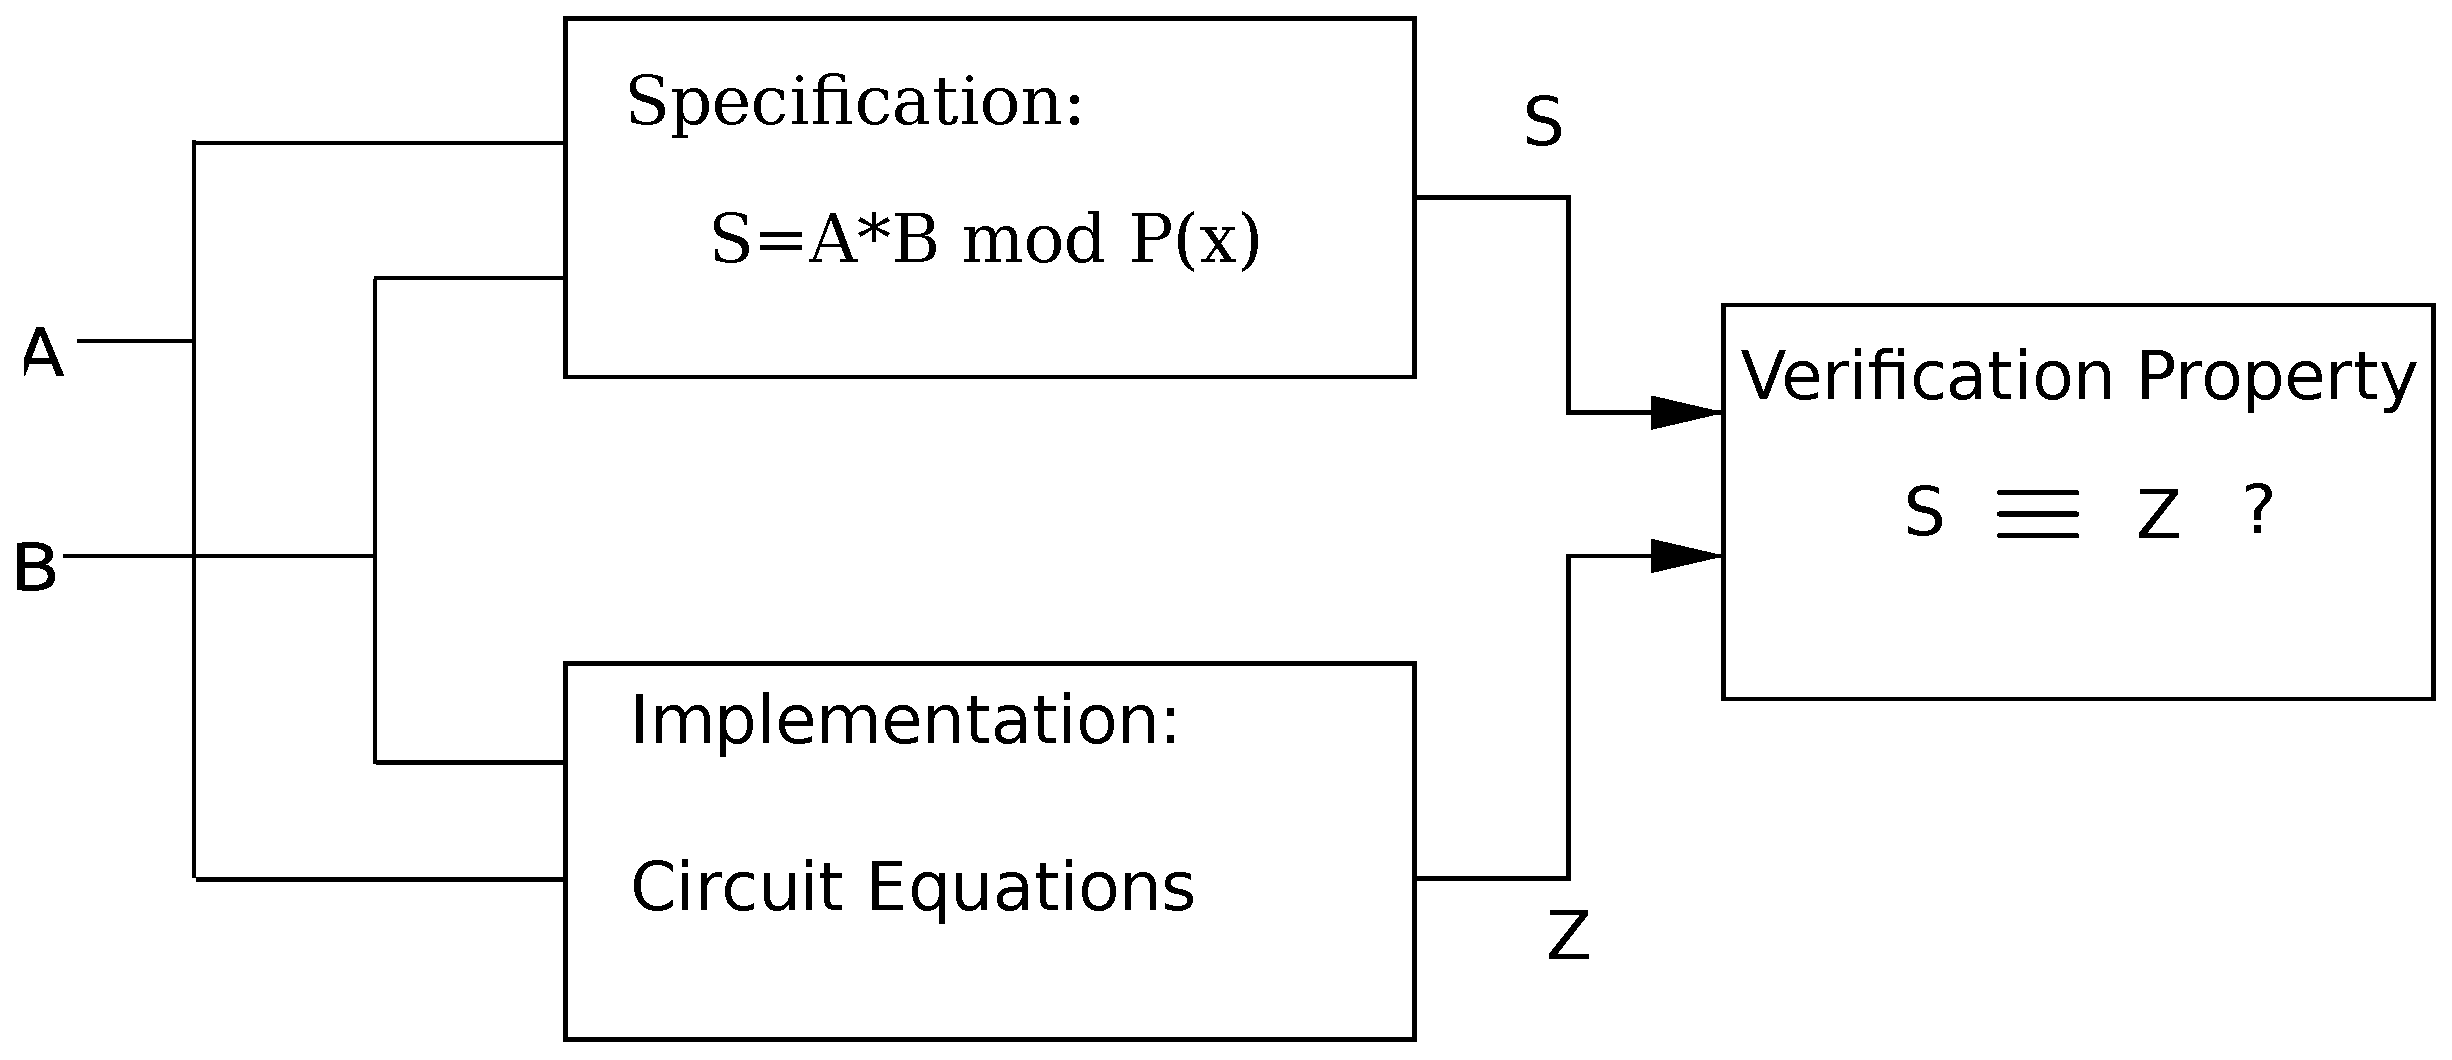
\includegraphics[scale=0.25]{./figures/setmember.eps}
}
\caption{The verification setup}
\label{fig:setup}
\end{figure}

{\bf Specification:} Given two $k$-bit inputs in bit-vector form
$A=(a_{k-1}a_{k-2}\cdots a_{1}a_{0})$ and $B=(b_{k-1}b_{k-2}\cdots
b_{1}b_{0})$, the specification can be modeled in polynomial forms in
$\mathbb{F}_{2^k}$ as follows: 

\begin{align}
A=&a_0+a_1\cdot \alpha+\cdots+a_{k-1}\cdot \alpha^{k-1} \nonumber \\
B=&b_0+b_1\cdot \alpha+\cdots+b_{k-1}\cdot \alpha^{k-1} \nonumber \\
S=&A\cdot B \pmod {P(x)} \nonumber
\end{align}

%where $A, B \in \mathbb{F}_{2^k} ~(a_i, b_i \in \mathbb{F}_{2})$ symbolically represent the inputs, 
%and $S\in \mathbb{F}_{2^k}$ represents the result of the multiplication. 

{\bf Implementation:} Given a gate-level circuit netlist, we map the gate-level
Boolean operators (AND, OR, NOT, XOR) to polynomials over
$\mathbb{F}_2 (\subset \mathbb{F}_{2^k})$ using the following
one-to-one mapping over $\mathbb{B} \rightarrow \mathbb{F}_2$ : 
\begin{equation}
\label{b2poly}
\begin{split}
\neg a\rightarrow a+1 \pmod 2  \\  
a \vee b \rightarrow a+b+a\cdot b \pmod 2  \\ 
a \wedge b \rightarrow a\cdot b \pmod 2  \\ 
a \oplus b \rightarrow a+b \pmod 2 
\end{split}
\end{equation}
where $a,b \in \mathbb{F}_{2}=\{0,1\}$.
Note that the equation $c=\mathcal{F}(a,b)$ is written in polynomial
form as $c-\mathcal{F}(a,b)=c+\mathcal{F}(a,b)$, ~as $-1 \equiv +1
\pmod 2$. 


 %a special mapping is the mapping of equation:
%\begin{equation}
%c=\mathcal{F}(a,b) \rightarrow c-\mathcal{F}(a,b)=0 \rightarrow c+\mathcal{F}(a,b)=0 \nonumber
%\end{equation}
%where $f$ represents any Boolean operator.

\begin{Example}
Consider the equation with Boolean operators: 
\begin{equation}
z=a \oplus (b \vee c). \nonumber
\end{equation}

The equation modeled over $\mathbb{F}_{2}$ is:
\begin{equation}
z+a + b + c + b\cdot c=0 \nonumber
\end{equation}  

The left-hand side expression is a polynomial in
$\mathbb{F}_{2}\left[a,b,c,z\right] \subset
\mathbb{F}_{2^{k}}\left[a,b,c,z\right]$: 
\begin{equation}
z+a + b + c + b\cdot c \nonumber
\end{equation}  
\end{Example}

Therefore, we can transform the entire circuit implementation as
polynomials over $\mathbb{F}_{2^k}$.  Let $Z$ symbolically denote the
word-level result of the implementation, i.e. the output of the
circuit.   

{\bf The Verification Property:}
The property $S=Z$ is modeled as a polynomial  $f: S+Z=0$ over
$\mathbb{F}_{2^k}$. 

Overall, our verification constraints can be modeled as a polynomial
system as follows:  

\begin{eqnarray}
 \left .  \begin{aligned}
f_1(x_1,x_2,\cdots, x_d)=0  \\
f_2(x_1,x_2,\cdots, x_d)=0  \\
\vdots  \\
%f_s(x_1,x_2,\cdots, x_d)=0  \\
f_{Z}: Z+z_{0}+z_{1}\cdot \alpha,\cdots,{z_{k-1}}\cdot \alpha^{k-1}=0   
 \end{aligned} 
\ \right\}
 &\qquad&  \text{\it Circuit implementation} \nonumber \\
 \left . \begin{aligned}
f_{A}:A+a_0+a_1\cdot \alpha+\cdots+a_{k-1}\cdot \alpha^{k-1}=0   \\ 
f_{B}:B+b_0+b_1\cdot \alpha+\cdots+b_{k-1}\cdot \alpha^{k-1}=0   \\ 
f_{spec}: S+A\cdot B =0   
 \end{aligned} 
\right\}
 &\qquad&  \text{\it Word-level specification} \nonumber \\
 \left .  \begin{aligned}
f:S+Z=0  \nonumber 
 \end{aligned} 
\right\}
 &\qquad& \text{Property:}~S = Z~?~
\end{eqnarray}


\begin{Example}
\label{exp:mul2bit}
Consider a 2-bit multiplier over ${\mathbb{F}}_{2^2}$ with
$P(x)=x^{2}+x+1$, given in Fig. \ref{fig:2bitmul}. Variables $a_0,
a_1, b_0, b_1$ are primary inputs, $z_0, z_1$ are primary outputs, and
$c_0, c_1, c_2, c_3, r_0$ are intermediate variables. The gate $\otimes$
corresponds to AND-gate, i.e. bit-level multiplication modulo 2. The
gate $\oplus$ corresponds to XOR-gate, i.e. addition modulo 2.

\begin{figure}[b]
\centerline{
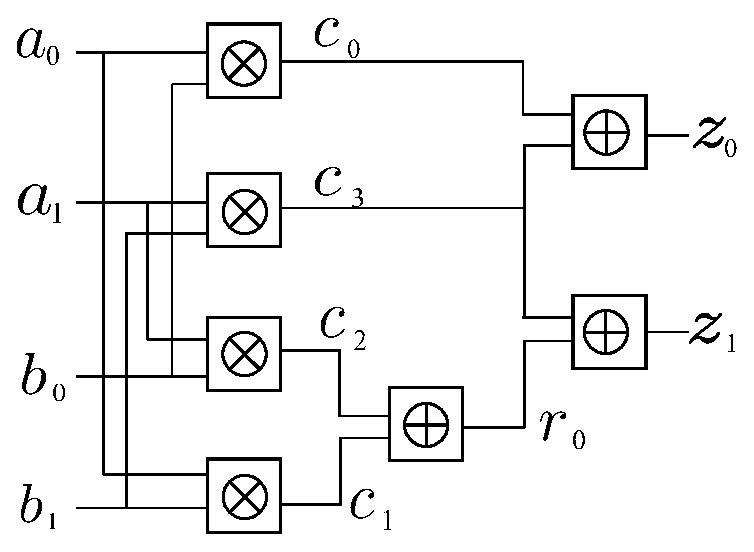
\includegraphics[scale=0.5]{./figures/2bitmultiplier.eps}
}
\caption{ A 2-bit multiplier over ${\mathbb{F}}(2^2)$.}
\label{fig:2bitmul}
\end{figure}

The circuit can be described using the following Boolean equations:
\begin{align*}
c_0=a_0 \wedge b_0,   \nonumber \\
c_1=a_0 \wedge b_1,   \nonumber \\
c_2=a_1 \wedge b_0, \nonumber \\
c_3=a_1 \wedge b_1,   \nonumber \\
r_0=c_1 \oplus c_2 ,      \nonumber \\
z_0=c_0 \oplus c_3,   \nonumber \\
z_1=r_0 \oplus c_3,    \nonumber
\end{align*}

With the mapping rules given in Equation \ref{b2poly}, 
the above equations are transformed into the following polynomials:
\begin{align*}
c_0+a_0 \cdot b_0,   \nonumber \\
c_1+a_0 \cdot b_1,   \nonumber \\
c_2+a_1 \cdot b_0,   \nonumber \\
c_3+a_1 \cdot b_1,   \nonumber \\
r_0+c_1 + c_2 ,      \nonumber \\
z_0+c_0 + c_3,   \nonumber \\
z_1+r_0 + c_3,   \nonumber
\end{align*}

Therefore, our overall polynomial system is:
\begin{eqnarray}
 \left .  \begin{aligned}
f_1: c_0+a_0 \cdot b_0  \\
f_2: c_1+a_0 \cdot b_1  \\
f_3: c_2+a_1 \cdot b_0  \\
f_4: c_3+a_1 \cdot b_1  \\
f_5: r_0+c_1 + c_2		\\
f_6: z_0+c_0 + c_3		\\
f_7: z_1+r_0 + c_3		\\
f_{Z}: Z+z_0+z_1\cdot \alpha   
 \end{aligned} 
\ \right\}
 &\qquad&  {\text {\it Circuit constraints}} \nonumber \\
 \left . \begin{aligned}
f_{A}: A+a_0+a_1\cdot \alpha  \\ 
f_{B}: B+b_0+b_1\cdot  \alpha  \\ 
f_{spec}: S+A\cdot B   
 \end{aligned} 
\right\}
 &\qquad&  {\text {\it specification}} \nonumber \\
 \left .  \begin{aligned}
f: S+Z  \nonumber 
 \end{aligned} 
\right\}
 &\qquad& \text{\it Property to verify:} ~S = Z~? 
\end{eqnarray}

\end{Example}

%As shown above, our verification problem is clearly algebraic in nature. 
%Therefore, the use of polynomial algebra is most suitable for such applications.

With the polynomial model given above, we formulate our problem as 
{\bf (radical) ideal membership testing},  which is described next.


%%%%%%%%%%%%%%%%%%%%%%%%%%%%%%%%%%%%%
%%%%%%%%%%%%%%%%%%%%%%%%%%%%%%%%%%%%%
%%%%%%%%%%%%%%%%%%%%%%%%%%%%%%%%%%%%%%%%
\section{Verification Formulation as Ideal Membership Testing}\label{sec:radicaltest}

%Given a specification polynomial $f: S + A\cdot B$ where $A =
%a_0 + a_1 \alpha + \dots + a_{k-1}\alpha^{k-1}, B = b_0 + b_1 \alpha +
%\dots + b_{k-1}\alpha^{k-1}$. 
%We are also given a gate-level circuit $Z$ with
%$\{a_0, \dots, a_{k-1}, ~b_0, \dots, b_{k-1}\}$ as primary inputs and
%$\{z_0, \dots, z_{k-1}\}$ as the primary outputs. We have to check if
%the circuit $Z$ implements the function $f$ over the given field
%$\mathbb{F}_{2^k}$. 

To formulate our verification test, we first analyze the circuit and
model the Boolean gate-level operators as polynomials over
$\mathbb{F}_2 ~(\subset \mathbb{F}_{2^k})$, as given by the
mappings of Equations \ref{b2poly}.  
To this set we then append the polynomials corresponding to the
word-level specification.  Let $\{f_1,f_2,\ldots,f_s\}$ denote this
set of polynomials derived from  both {\it specification} and {\it
  implementation}.  
%$A + a_0 + a_1\alpha + \dots + a_{k-1}\alpha^{k-1}$, 
%$B + b_0 + b_1\alpha + \dots b_{k-1}\alpha^{k-1}$, 
%$Z + z_0 + z_1 \alpha + \dots + z_{k-1}\alpha^{k-1}$; 
%these polynomials specify the correspondence between the bit-level ($\mathbb{F}_2$) 
%and the word-level ($\mathbb{F}_{2^k}$) variables in the system. 
%We denote these constraints as polynomials $\{f_1, \dots, f_s\}$ over
%the ring $\mathbb{F}_{2^k}[x_1,\dots, x_d]$, 
Let $\{x_1,x_2,\ldots,x_d\}$ denote all the variables in the
polynomial system. As a consequence, $\{f_1,f_2,\ldots,f_s\}\in
\mathbb{F}_{2^k}[x_{1},\dots,x_{d}]$. Let $J = \langle f_1,
\dots,f_s\rangle \subset \mathbb{F}_{2^k}[x_{1},\dots,x_{d}]$ denote
the ideal generated by these polynomials. Our verification property
$S=Z$ is also modeled as a polynomial $f: S+Z \in
\mathbb{F}_{2^k}[x_{1},\dots,x_{d}]$. 
% (Note $S=G$ is not included)
%Let $\{x_1,x_2,\ldots,x_d\}$ denote all variables occurring in {\it specification} and {\it implementation}, where $x_i\in \mathbb{F}_2 \subset \mathbb{F}_{2^k}$.
%We denote the generated ideal as $J = \langle f_1, \dots,f_s\rangle$.  

To prove that the specification polynomial ($f$) matches the
implementation ($J = \langle f_1, \dots, f_s\rangle$), we need to
check whether $f: S+Z=0$  {\it agrees} with all the solutions of $J$
over the field $\mathbb{F}_{2^k}$. In computer algebra terminology, we
need to check {\it whether or not $f$ vanishes on the variety
  $V_{\mathbb{F}_{2^k}}(J)$},  where $V_{\mathbb{F}_{2^k}}(J)$ denotes
the variety of ideal $J$ over the given field $\mathbb{F}_{2^k}$.
This is because for all points (solutions) $p \in
V_{\mathbb{F}_{2^k}}(J)$, if $f(p) = 0$, then $f: S + Z = 0 \implies S
=Z$. On the other hand, if $f(p) \neq 0$ for some point $p$, then $p$
corresponds to the bug in the design.  

Now if $f$ vanishes on $V_{\mathbb{F}_{2^k}}(J)$, according to
Proposition \ref{pro:iofv},  we know that $f$ should be a member of
the radical ideal $I(V_{\mathbb{F}_{2^k}}(J))$.  Therefore, our
verification test can be modeled as membership testing of $f$ in the
(radical) ideal $I(V_{\mathbb{F}_{2^k}}(J))$. To solve this problem,
we need to first derive the generators of $I(V_{\mathbb{F}_{2^k}}(J))$ 
(note that we are only given the generators of $J$), and then perform
the ideal membership testing using the Gr\"obner basis algorithm.  

\subsection{Generating $I(V_{\mathbb{F}_{2^k}}(J))$}
Strong Nullstellensatz establishes correspondences between ideals and their radicals.
As given in Theorem \ref{thm:sns},  $I(V_{\overline {\mathbb{K}}}(J)) =\sqrt{J}$, where 
the variety $V$ is taken over the algebraically closed field
$\overline {\mathbb{K}}$. Finite fields are, however, {\it not}
algebraically closed, as shown by the following result from
\cite{galois_field:mceliece}:  

\begin{Theorem}
Given finite fields $\mathbb{F}_{2^n}$ and $\mathbb{F}_{2^m}$ such that $n$ divides
$m$. Then $\mathbb{F}_{2^n} \subset \mathbb{F}_{2^m}$.
\end{Theorem}

Therefore, $\mathbb{F}_2 \subset \mathbb{F}_{2^2} \subset
\mathbb{F}_{2^4} \subset \mathbb{F}_{2^8} \subset \dots$; and
$\mathbb{F}_2 \subset \mathbb{F}_{2^3} \subset \mathbb{F}_{2^6}  \dots
$; and so on. The algebraic closure of $\mathbb{F}_{2^k}$ is known to
be  an infinite field obtained as the union of all such finite fields.  


Therefore, Nullstellensatz needs to be suitably modified for
application over finite fields. 
%Let $\overline {\mathbb{F}_{2^k}}$ denote the algebraic closure of $\mathbb{F}_{2^k}$.
We re-visit the notion of vanishing polynomials for this purpose. 

Over the finite field $\mathbb{F}_{2^k}$, any element $A$ satisfies
the property $A^{2^k}-A=0$. Therefore, polynomial  $x^{2^k}-x$
vanishes at all points in $\mathbb{F}_{2^k}$, and $x^{2^k}-x$ is
called the vanishing polynomial of the field. As a consequence, the
variety $V(x^{2^k}-x)=\mathbb{F}_{2^k}$. Over multivariate polynomial
ring $\mathbb{F}_{2^k}[x_1,\dots,x_d]$,
$V(x_1^{2^k}-x_1,\dots,x_d^{2^k}-x_d)$ is $\mathbb{F}_{2^k}^d$. 
 
In the sequel, we use the following notation: 
Let $J_0=\langle x_1^{2^k}-x_1,\dots,x_d^{2^k}-x_d \rangle $ denote
the ideal of vanishing polynomials over $\mathbb{F}_{2^k}$. Also, if
$J=\langle f_1,\dots,f_s \rangle$ 
%and  $J_0=\langle x_1^{2^k}-x_1,\dots,x_d^{2^k}-x_d \rangle $, 
then the sum of ideals $J+J_0=\langle f_1,\dots,f_s ,
~~x_1^{2^k}-x_1,\dots,x_d^{2^k}-x_d \rangle$.  Let $\overline
{\mathbb{F}_{2^k}}$ denote the algebraic closure of
$\mathbb{F}_{2^k}$. 

\begin{Lemma} \label{lem:closure}
Let $J \subset \mathbb{F}_{2^k}[x_1,\dots,x_d]$ be any ideal and let
$J_0=\langle x_1^{2^k}-x_1,\dots,x_d^{2^k}-x_d \rangle$. Then
$V_{\mathbb{F}_{2^k}}(J)=V_{\overline {\mathbb{F}_{2^k}}}(J+J_0)$. 
\end{Lemma}

\begin{Proof}
 Since $\overline {\mathbb{F}_{2^k}} \supset \mathbb{F}_{2^k}$, we have :

\begin{eqnarray}
V_{\mathbb{F}_{2^k}}(J) &= & V_{\overline {\mathbb{F}_{2^k}}}(J) \cap \mathbb{F}_{2^k}^d  \nonumber \\
 		   &= & V_{\overline {\mathbb{F}_{2^k}}}(J) \cap  V_{\mathbb{F}_{2^k}}(J_0)  \nonumber \\
 		   &= &  V_{\overline {\mathbb{F}_{2^k}}}(J) \cap  V_{\overline{\mathbb{F}_{2^k}}}(J_0) \nonumber  \\
		   &= & V_{\overline {\mathbb{F}_{2^k}}}(J+J_0) \nonumber
\end{eqnarray}
\end{Proof}

As a consequence of the above lemma, variety of any ideal $J$ over a
finite field $\mathbb{F}_{2^k}$ can be equivalently  analyzed over its
algebraic closure $\overline {\mathbb{F}_{2^k}}$ by just appending to
$J$ all the vanishing polynomials $J_0$. These vanishing polynomials
do not change the zero-set of $J$ but allow the same analysis over the
algebraic closure. 

\begin{Lemma}\label{lem:selfrad}
$I(V_{\mathbb{F}_{2^k}}(J))=I(V_{\overline {\mathbb{F}_{2^k}}}(J+J_0))=\sqrt {J+J_0}$.
\end{Lemma}

\begin{Proof}
As shown above, $V_{\mathbb{F}_{2^k}}(J)=V_{\overline {\mathbb{F}_{2^k}}}(J+J_0)$.
Therefore, $I(V_{\mathbb{F}_{2^k}}(J))=I(V_{\overline {\mathbb{F}_{2^k}}}(J+J_0))$.
According to Strong Nullstellensatz, $I(V_{\overline
  {\mathbb{F}_{2^k}}}(J+J_0))=\sqrt {J+J_0}$. Thus: 
\begin{equation}
I(V_{\mathbb{F}_{2^k}}(J))=I(V_{\overline {\mathbb{F}_{2^k}}}(J+J_0))=\sqrt {J+J_0}
\end{equation}
\end{Proof}

\begin{Lemma}\label{lem:root}
Let $J$ be any arbitrary polynomial ideal in
$\mathbb{F}_{2^k}[x_1,\dots,x_d]$ and $J_0$ be the corresponding
vanishing ideal. Then $J+J_0$ is radical. In other words, $\sqrt
{J+J_0}=J+J_0$. 
\end{Lemma}
\begin{Proof}
This is a well known result, a proof of which is given in
\cite{gao:gf-gb-ms}. 
\end{Proof}

Putting together the above results, we finally arrive at the following
application of Nullstellensatz over finite fields.

%%%%%%%%%%%%%%%%strong nullstellensatz in finite field%%%%%%%%%%%%%
\begin{Theorem}\label{thm:snff}
$\left[\bf{Strong\  Nullstellensatz\ in\ Finite\ Fields}\right]$ Let
$J \subset \mathbb{F}_{2^k}[x_1, x_2, \cdots, x_n]$ be an ideal and
$J_0$ be the ideal of vanishing polynomials. Then, 
\begin{equation}
I(V_{\mathbb{F}_{2^k}}(J))=J+J_0=J+\langle x_1^{2^k}-x_1,x_2^{2^k}-x_2,\cdots, x_d^{2^k}-x_d\rangle
\end{equation}
\end{Theorem} 

\begin{Proof}
Combining Lemma \ref{lem:selfrad} and Lemma \ref{lem:root}, 
\begin{equation}
I(V_{\mathbb{F}_{2^k}}(J))=I(V_{\overline {\mathbb{F}_{2^k}}}(J+J_0))=\sqrt {J+J_0}=J+J_0
\end{equation}
where $J_0=\langle x_1^{2^k}-x_1,x_2^{2^k}-x_2,\cdots, x_d^{2^k}-x_d\rangle$.
\end{Proof}

{\bf Overall Verification Problem Formulation:} Through Strong
Nullstellensatz over finite fields, given an ideal $J$, we can
directly construct ideal $I(V_{\mathbb{F}_{2^k}}(J))=J+J_0$.  For our
verification problem, we take the polynomials $\{f_1, \dots, f_s\}$
representing the circuit constraints and the specification polynomials
to generate ideal $J$. Then we append the vanishing polynomials
$\{x_1^{2^k} - x_1, \dots, x_d^{2^k} - x_d\}$ of ideal $J_0$. Our
verification problem can now be formulated as testing whether the
verification property polynomial $f$ is in $J+J_0$. If $f \in (J +
J_0)$, correctness of the circuit is established. Otherwise, there is
a bug in the design. To test if $f \in (J + J_0)$, it is required to
compute a Gr\"obner  basis $G$ of the ideal $J+J_0$.  Then, we reduce
$f$ w.r.t. $G$: i.e., $f \stackrel{G}{\textstyle\longrightarrow}_+
r$. If $r=0$, then the circuit is correct, otherwise there is a bug in
the design.  


%Strong Nullstellensatz tells us $I(V(J)) =\sqrt{J}$. However, the result only 
%works over an algebraically closed field while finite fields are not an algebraically closed field.
%To solve this problem, an analogue in finite field $F_{2^k}$ of Strong Nullstellensatz is introduced here. 

%\begin{proof}
%Firstly, we need prove $J+\langle x_1^{2^k}-x_1,x_2^{2^k}-x_2,\cdots,x_d^{2^k}-x_d\rangle$ is radical. For convenience, let $q$ denote $2^k$, 
%let $I=J+\langle x_1^{2^k}-x_1,x_2^{2^k}-x_2,\cdots,x_d^{2^k}-x_d\rangle$.

%From Definition. \ref{def:radical}, we claim: 

%$f^m\in J \Rightarrow f\in J$, for some $m>0$.

%Let $I_0$ denoted $\langle x_i^q-x_i\rangle$. 
%Let $R$ denote $\mathbb{F}_q\left[x_1,x_2,\cdots,x_d\right]$.

%$\frac{R}{I_0}=\mathbb{F}_q\left[\overline x_i \mid {\overline x_i}^q=\overline x_i \right]$, 
%which means all variables have degree less than q in $\frac{R}{I_0}$.
%\begin{equation} \label{proofbasis}
%\forall g\in I_0\ \Leftrightarrow \ \bar{g}=0,\ where \bar{g}\in \frac{R}{I_0}.
%\end{equation}

%Let $g'=f^q-f$, where $f\in I$ .

%$\overline {f^q-f}=\overline {f^q}-\overline{f}$.

%$f\in I$ can be denoted as:
%\begin{equation}
%f=\displaystyle\sum\limits_{i=1}^n{a_i\cdot x_1^{i_1} \cdot x_2^{i_2} \cdots \cdot x_n^{i_n}}. \nonumber 
%\end{equation}

%then we can have the following two equations:
%\begin{equation}\label{fq}
%f^q=\displaystyle\sum\limits_{i=1}^n{a_i^q\cdot (x_1^q)^{i_1} \cdot (x_2^q)^{i_2} \cdots \cdot x_n^{i_n}}=\overline f. 
%\end{equation}
%\begin{equation}\label{fqbar}
%\overline {f^q}=\displaystyle\sum\limits_{i=1}^n{a_i^q\cdot (x_1^q)^{i_1} \cdot (x_2^q)^{i_2} \cdots \cdot x_n^{i_n}}. 
%\end{equation}

%From Eqn.\ref{fq} and Eqn.\ref{fqbar}, we can get
%\begin{equation}
%\overline {f^q}=\overline f \  \Leftrightarrow \ \overline {f^q}-\overline f=0 
%\end{equation}

%Then from Eqn.\ref{proofbasis}, we can have $f^q-f\ \in I_0 $, which then generates $(f^q-f)^q=f^{q^2}-f^q \in I_0$.

%\begin{equation}
 %\left.\begin{aligned}
        %f^q-f \in I_0 \\
        %f^{q^2}-f^q \in I_0
       %\end{aligned}
 %\right\}
 %\qquad  \Longrightarrow {f^{q^2}-f \in I_0} \nonumber
%\end{equation}

%Iteratively, we can have $\forall k\in\{0,1,2,\cdots\}, f^{q^k}-f\in I_0$.

%Then $\exists k',q^{k'} \ge m$, such that $f^m\in I \Rightarrow f^{q^k}\in I$.

%$f$ can be expressed as:

%$f=\underbrace{f-f^{q^k}}_{\in I_0 \subset I}+\underbrace{f^{q^k}}_{\in I}$.

%Now our claim is justified: if $f^m\in I$, then $f\in I$. In other words, $\sqrt{J+I_0}=J+I_0$.

%Secondly, we need prove $I(V(J))=J+I_0$.

%From Strong Nullstellensatz, we have:

%$I(V_{\overline {\mathbb{F}_q}}(J+I_0))=\sqrt{J+I_0}=J+I_0$.

%Notice $V_{\overline {\mathbb{F}_q}}(J+I_0)=V_{\mathbb{F}_q}(J)$.

%So we finally have $I(V_{\mathbb{F}_q}(J))=\sqrt{J+I_0}=J+I_0$. \hfill $\square$

%\end{proof}

%%%%%%%%%%%%%%%%%%%%%%%%%%%%%%%%%%%%%%%%%%%%%%%%%%%%%%%%%%%%

%Strong Nullstellensatz over $\mathbb{F}_{2^k}$ (Theorem \ref{thm:snff}) states this:
%\begin{equation}
 %I(V_{\mathbb{F}_{2^k}}(J)) = J + J_0 = \langle f_1, \dots, f_s, ~x_1^q-x_1, \dots, x_d^q - x_d\rangle. 
%\end{equation}
%Therefore, {\it we need to test whether or not $f$ is a member of the ideal $J + J_0$.}  


\begin{Example}
Let us re-consider Example \ref{exp:mul2bit}. First, polynomials are
extracted from the circuit implementation and the specification, as
shown in Example \ref{exp:mul2bit}. These polynomials represent the
ideal $J$. Along with the ideal $J_0=\langle x_1^{2^k}-x_1, \dots,
x_d^{2^k} - x_d \rangle$, the following polynomials represent $J+J_0$
for the multiplier circuit. 

\begin{eqnarray}
 \left .  
	\begin{aligned}
		f_1:c_0+a_0 \cdot b_0  \\
		f_2:c_1+a_0 \cdot b_1  \\
		f_3:c_2+a_1 \cdot b_0  \\
		f_4:c_3+a_1 \cdot b_1  \\
		f_5:r_0+c_1 + c_2		\\
		f_6:z_0+c_0 + c_3		\\
		f_7:z_1+r_0 + c_3		\\
		f_{Z}:Z+z_0+z_1\cdot \alpha   
	\end{aligned} 
 \ \right\}
 &\qquad&  {\it implementation ~(\subset J)} \nonumber \\
 \left . 
	\begin{aligned}
		f_{A}:A+a_0+a_1\cdot \alpha   \\ 
		f_{B}:B+b_0+b_1\cdot \alpha  \\ 
		f_{spec}:S+A\cdot B =0   
	\end{aligned} 
 \right\}
 &\qquad&  {\it specification ~(\subset J)} \nonumber \\
  \left . 
	\begin{aligned}
		a_0^2-a_0, ~a_1^2-a_1,~b_0^2-b_0, ~b_1^2-b_1   \\ 
		c_0^2-c_0, ~c_1^2-c_1,~c_2^2-c_2, ~c_3^2-c_3  \\ 
		r_0^2-r_0, ~z_0^2-z_0,~z_1^2-z_1    \\ 
		A^4-A, ~B^4-B ,~Z^4-Z,~ S^4-S		  
	\end{aligned} 
 \right\}
 &\qquad&  {\it \text{vanishing polynomials} (J_0)} \nonumber
\end{eqnarray}

Now we need to compute the Gr\"obner basis $G$ of this ideal
$J+J_0$. Once the computation of $G$ is completed, we simply need a
polynomial reduction to test whether $f: S+Z$ can be reduced by
$G$. In other words, we need test whether
$S+Z\stackrel{G}{\textstyle\longrightarrow}_+ 0$? 
\end{Example}



While our approach seems reasonably simple, the complexity of
Gr\"obner basis computation can make verification infeasible. 


%: first computing a Gr\"obner basis and then conducting a polynomial reduction. 
%Unfortunately, two problems regarding Gr\"obner basis computation arises: one is related to the complexity of Gr\"obner basis computation;
%the other one is related to the degree representation of vanishing polynomials.

%The Gr\"obner basis computation is known to have double-exponential worst-case complexity in the input data.
%Even over finite fields, the complexity still makes this approach impractical.

{\bf Complexity of Gr\"obner basis over finite fields:} For our
specific problem of computing a Gr\"obner basis for $J + J_0$ over
$\mathbb{F}_{q}$, the following result is known \cite{gao:gf-gb-ms}:

\begin{Theorem}\label{thm:gb-complexity}
Let $I = \langle f_1, \dots, f_s, ~x_1^q - x_1, \dots, x_d^q -
x_d\rangle \subset \mathbb{F}_{q}[x_1, \dots, x_d]$ be an ideal over
any finite field $\mathbb{F}_{q}$. The time and space complexity of
Buchberger's algorithm to compute a Gr\"obner basis of $I$ is bounded
by $q^{O(d)}$ assuming that the length of input $f_1, \dots, f_s$ is
dominated by $q^{O(d)}$.  
\end{Theorem}

In our case $q = 2^k$, and when $k$ and $d$ are large, this complexity
makes verification infeasible. 
%The second problem results from the degree representation of vanishing polynomials over large field. 
%Vanishing polynomials ($x_i^q - x_i$) introduce a practical problem. 
%Most computer algebra tools (Gr\"obner Bases engines) have a bound on the degree of variables in the system. 
%For our work, we use the {\sc Singular} \cite{DGPS} tool. 
%{\sc Singular} has a limitation that the degree of a variable ($q$ in $x^q$) be
%$<2^{16}$. In cryptography, one encounters very large fields $F_q$ where $q =
%2^{256}$ or higher. So we need to be able to find alternate ways to
%account for the high degree polynomials $x^q - x$ in $J_0$. 
%These two practical problems hinders the practical application of our approach.
%In subsequent sections, we offer our solutions to these problems.
In what follows, we show that a variable/term order can be derived by
analyzing the circuit topology which makes the set of polynomials
$\{f_1, \dots,f_s, x_1^{2^k} - x_1, \dots, x_d^{2^k} - x_d\}$ itself a
Gr\"obner basis of $J+J_0$ -- obviating the need to apply Buchberger's
algorithm. 

%%%%%%%%%%%%%%%%%%%%%%%%%%%%%%%%%%%%%%%%%%%%%%
%%%%%%%%%%%%  New Section  %%%%%%%%%%%%%%%%%%%
\section{Obviating Buchberger's Algorithm}
\label{sec:improv}

Just as variable orderings play a critical role in constructing BDDs
and solving SAT feasibly,  the Gr\"obner basis computation is also
highly susceptible to the term orderings imposed on the polynomials. 
Therefore a key step to improve/avoid the high complexity 
of Gr\"obner basis computation is to derive a ``good" term order.
%But unlike that there is no best variable order for SAT/BDD, there
%does exist an optimal variable order %for Gr\"obner basis computation
%in our case. With such an optimal variable order,  %the expensive
%computation of Gr\"obner basis can be obviated. 

Buchberger's work \cite{buchberger_thesis} initially laid the
foundation for computing Gr\"obner's bases.  Subsequently, many
improvements were introduced to improve the efficiency of Buchberger's
algorithm. Two of the most important improvements are the chain and
product criteria. For our particular circuit verification application,
we exploit the product criteria. 


\begin{Lemma}
\label{lemma:prodcriteria}
[Product Criterion \cite{productc:1979}] Let $\mathbb{F}$ be any
field, and $f, g \in \mathbb{F}[x_1,\cdots,x_d]$ be polynomials. If
the equality $lm(f) \cdot lm(g) = LCM(lm(f), lm(g))$ holds, then
$Spoly(f,g)\stackrel{G}{\textstyle\longrightarrow}_+ 0.$ 
\end{Lemma}

The above result states that when the leading monomials of $f, g$ are
relatively prime, then $Spoly(f, g)$ always reduces to 0 modulo $G$. Thus
$Spoly(f, g)$ need not be considered in Buchberger's algorithm. 
Modern computer algebra engines perform this check to avoid
unnecessary $Spoly(f, g)$ computations.  If we could analyze the given
circuit and  derive a term order such that every polynomial pair
($f,g$) in the generating set has relatively prime leading monomials,
then for all S-polynomials, the subsequent reduction would not add any
new polynomials in the basis. In other words, $Spoly(f, g)
\stackrel{G}{\textstyle\longrightarrow}_+ 0$ for all pairs $f,
g$. Consequently, the polynomials $\{f_1, \dots, f_s\}$ extracted from
the circuit (corresponding ideal $J$) and represented using such a
term order would itself constitute a Gr\"obner basis of $J$.  In
\cite{wienand:cav08}, the authors derive exactly such a term order,
and a similar concept can be applied in our case. 

Note that in our case: 
\begin{itemize}
\item since the circuit constraints $\{f_1, \dots,f_s\}$ are modeled
  as polynomials in $\mathbb{F}_2 \subset {\mathbb{F}}_{2^k}$,  they
  contain only multi-linear monomial terms;  
\item the output of a gate is uniquely computed, and it always appears
  as a ``single variable term'' in the 	polynomials; 
\item the circuit is acyclic;
\end{itemize}

Let $x_i$ be the output variable of any gate $H_i$ in the circuit, and
let $x_{p_1}, \dots,x_{p_j}$ denote variables that are the inputs to
the gate $H_i$.  If we can represent the polynomials $f_i$ such that
$x_i >$ every monomial  in the variables $x_{p_1}, \dots, x_{p_j}$,
then all $(f_i, f_j), i\neq j$ have  relatively prime leading
monomials and $\{f_1, \dots, f_s\}$ is a Gr\"obner basis. 
% (this is Proposition 2 in \cite{wienand:cav08}). 

\begin{Proposition} \label{prop:top-order}
Let $C$ be any arbitrary combinational circuit. Let $\{x_1, \dots,
x_d\}$ denote the set of all variables (signals) in the circuit,
i.e. the primary input, intermediate and primary output
variables. Perform a {\bf reverse topological traversal} of the
circuit and order the variables such that $x_i > x_j$ if $x_i$ appears
earlier in the reverse topological order. Impose a lex term order to
represent the Boolean expression for each gate as a polynomial $f_i$;
then $f_i = x_i + \text{tail}(f_i)$. Then the set of all polynomials
$\{f_1, \dots, f_s\}$ forms a Gr\"obner basis, as $lt(f_i)$ and $
lt(f_j)$ for $i\neq j$ are relatively prime. 
\end{Proposition}
	
\begin{Example}
Consider the circuit of Figure \ref{fig:2bitmul}, reproduced
below. Variables $a_0, a_1, b_0, b_1$ are primary inputs,  $z_0, z_1$
are primary outputs, and $c_0, c_1, c_2, c_3, r_0$ are intermediate
variables.   

\begin{figure}[htb]
\centerline{
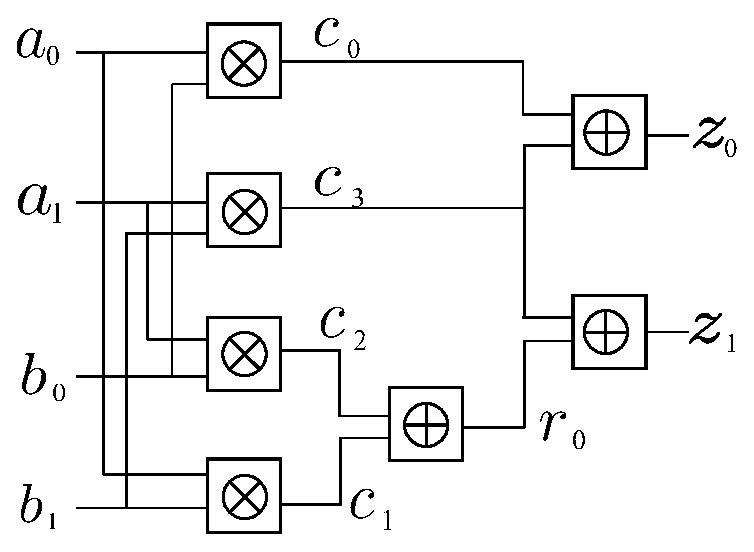
\includegraphics[scale=0.4]{./figures/2bitmultiplier.eps}
}
\caption{ A 2-bit multiplier over ${\mathbb{F}}(2^2)$. The gate $\otimes$
corresponds to AND-gate, i.e. bit-level multiplication modulo 2. The
gate $\oplus$ corresponds to XOR-gate, i.e. addition modulo 2.}
\label{fig:mul2bit2nd}
\end{figure}

We perform a reverse topological traversal of the
circuit. Starting from the primary outputs, traverse the circuit 
to the primary inputs, and order the gates according to the their
(reverse) topological levels. The primary outputs $z_0,
z_1$ are both at level-0, variables $r_0, c_0, c_3$ are at
level-1, ~$c_1, c_2$ are at level-2, and the primary inputs
$a_0, a_1, b_0, b_1$ are at level-3. We order the variables $\{z_0 >
z_1\} > \{r_0 > c_0 > c_3\} > \{c_1 > c_2\} > \{a_0 > a_1 >  b_0 >
b_1\}$. Using this variable order, we impose a {\it lex} term order on
the monomials. Then the polynomials of $J$ all have relatively prime 
leading terms, as shown below: 

\begin{align*}
c_0+a_0 \cdot b_0, \ lm=c_0;  \nonumber \\
c_1+a_0 \cdot b_1, \ lm=c_1;  \nonumber \\
c_2+a_1 \cdot b_0, \ lm=c_2;  \nonumber \\
c_3+a_1 \cdot b_1, \ lm=c_3;  \nonumber \\
r_0+c_1 + s_2 , \ lm=r_0;     \nonumber \\
z_0+c_0 \cdot c_3, \ lm=z_0;  \nonumber \\
z_1+r_0 \cdot c_3, \ lm=z_1   \nonumber
\end{align*}


In our overall problem formulation, we also have variables $A, B, S, Z
\in \mathbb{F}_{2^k}$.  They can also be accommodated in this term
order by imposing $S >Z> A > B > z_0 > z_1 > r_0 > c_0 > c_3 > c_1 >
c_2 > a_0 > a_1 >b_0 > b_1$. 
\end{Example}

Thus, using the result of Proposition \ref{prop:top-order}, the set
of polynomials $\{f_1, \dots, f_s\}$ is a Gr\"obner basis for
$J$. Note that  $\{x_1^{2^k} - x_1, \dots, x_d^{2^k}
- x_d\}$ is a Gr\"obner basis for $J_0$. However, we have to compute a
Gr\"obner basis of $J + J_0 = \langle f_1, \dots, f_s, ~x_1^{2^k} - x_1,
\dots, x_d^{2^k} - x_d \rangle$.  Not all polynomials pairs in $\{f_1,
\dots, f_s, ~x_1^{2^k} - x_1, \dots, x_d^{2^k} - x_d\}$ have
relatively prime leading monomials.  

Consider an arbitrary polynomial $f_i \in J$. Using our term order, we
have $f_i = x_i + \text{tail}(f_i)$; i.e. the leading monomial of
$f_i$ is a single variable term $x_i$. Clearly, the pair
$(x_i+\text{tail}(f_i), ~x_i^{2^k}-x_i), ~f_i \in J, ~x_i^{2^k} - x_i \in J_0$
do not have relatively prime leading monomials. In fact, the pairs
$(x_i+\text{tail}(f_i), x_i^{2^k}-x_i)$ are the only ones to be considered
for Gr\"obner basis computation, as all other pairs have relatively
prime leading terms. This motivated us to investigate further the
question ``what is the result of the reduction
$\text{Spoly}(x_i+\text{tail}(f_i), x_i^{2^k}-x_i) 
\stackrel{J,J_0}{\longrightarrow}_+ r $?''. We state and prove the
following: 

\begin{Theorem}
\label{thm:contrib}
Let $q = 2^k$, and let $\mathbb{F}_q[x_1, \ldots, x_d]$ be a ring on
which we have a monomial order $>$. Let $I$ be a subset of $\{1,
\ldots, d\}$. For all $i \in I$, let $f_i = x_i +P_i$ (where $P_i =
\text{tail}(f_i)$) such that  all indeterminates $x_j$  that appear in
$P_i$ satisfy $x_i > x_j$.  Then the set $G = \{f_i :  i  \in I\} \cup
\{x_1^q-x_1, \ldots, x_d^q-x_d\}$ is a Gr\"obner basis.  
\end{Theorem}

\begin{Proof}
According to Buchberger's Theorem (Theorem 1.7.4 in \cite{gb_book}),
we need to show that for all $f, g \in G$, $Spoly(f,g)
\stackrel{G}{\rightarrow}_+ 0$. Let $G_1=\{ f_i : i \in I \}$. Lemma
\ref{lemma:prodcriteria} shows that if $f, g \in G$, have relatively
prime leading terms, then  $Spoly(f,g) \stackrel{G}{\rightarrow}_+
0$. So the only case where Lemma \ref{lemma:prodcriteria} does not
apply is when $f = x_i + P_i$ and $g = x_i^q-x_i$. Then $Spoly(f,g)=
x_i^{q-1} f - g = P_i x_i^{q-1} + x_i$. In what follows, it is important
to note that the indeterminates appearing in $P_i$ are all less than
$x_i$.  

First of all,  $P_i x_i^{q-1} +x_i -
P_ix_i^{q-2}(x_i+P_i)=P_i^2x_i^{q-2} +x_i,$ which shows that $P_i 
x_i^{q-1} +x_i \stackrel{x_i+P_i}{\longrightarrow}  P_i ^2x_i^{q-2}
+x_i.$  

Next, $P_i^2 x_i^{q-2} + x_i  - P_i^2x_i^{q-3}(x_i+P_i)=
P_i^3x_i^{q-3}+ x_i.$ Continuing in this fashion, we get $P_i^{q-1}x_i
+x_i -P_i^{q-1}(x_i+P_i) = x_i + P_i^q,$ and finally 
$x_i+P_i^q -(x_i+P_i) = P_i^q-P_i.$ Hence, 
$$P_i x_i^{q-1} +x_i \stackrel{x_i+P_i}{\longrightarrow}  P_i
^2x_i^{q-2} +x_i \stackrel{x_i+P_i}{\longrightarrow} P_i ^3x_i^{q-3}
+x_i \stackrel{x_i+P_i}{\longrightarrow} \cdots$$
$$\cdots \stackrel{x_i+P_i}{\longrightarrow}
P_i^q+x_i\stackrel{x_i+P_i}{\longrightarrow} P_i^q-P_i.$$ 


Over the finite field $\mathbb{F}_{q}$, $P_i^q-P_i$ is a vanishing
polynomial. Therefore, $P_i^q-P_i \in I(V(J_0))= \langle
x_1^q-x_1, \ldots, x_d^q-x_d\rangle$. By Lemma
\ref{lemma:prodcriteria}, $G_0=\{x_1^q-x_1, \ldots, x_d^q-x_d\}$ is
Gr\"obner basis. Therefore %So, Theorem 1.6.2 in~\cite{AL} shows that
$P_i^q-P_i \stackrel{G_0}\rightarrow_+ 0$ which gives that $P_i^q-P_i
\stackrel{G}\rightarrow_+ 0$, as $G_0 \subset G$. 

In conclusion, $\forall f, g \in G, ~Spoly(f,g)
\stackrel{G}\rightarrow _+0$ and hence $G$ is a Gr\"obner basis.
\end{Proof}

As a consequence of Theorem \ref{thm:contrib}, the Gr\"obner basis $G$
for our verification instance (ideal $J + J_0$) can be obtained
directly by construction using a reverse topological traversal of the
circuit.  While $G$ is indeed a Gr\"obner basis, it is neither {\it
  minimal} nor {\it reduced}. We now show that this basis can actually
be made {\it minimal} by considering the vanishing ideal of only the
primary inputs of the given circuit. 

%A Gr\"obner basis can be further simplified to its minimal form.
%\begin{Definition}
%\label{def:minimal}
%A minimal Gr\"obner basis for a polynomial ideal $I$ is a Gr\"obner basis $G$ for $I$ such that:
%\begin{itemize}
%	\item $lc(p) = 1$ $\forall p \in G$.
%	\item $\forall  p \in G$, $lm(p) \in lm(G-\{p\})$.
%\end{itemize}
%\end{Definition}



% Note that the minimal Gr\"obner basis has the same variety as its original Gr\"obner basis. 
% Therefore their solution space is the same.
% Following this definition, we can have a minimal Gr\"obner basis for a circuit.

\begin{Corollary}
\label{thm:mini}
Let $q = 2^k$ and $\mathbb{F}_q[x_1, \ldots, x_d]$ be the ring on
which we impose the monomial order $>$ obtained via Proposition
\ref{prop:top-order}. Let $I$ be a subset of $\{1, \ldots, d\}$. For
all $i \in I$, let $f_i = x_i +P_i$ (where $P_i = \text{tail}(f_i)$) such
that  all indeterminates $x_j$  that appear in $P_i$ satisfy $x_i >
x_j$.  Let $X_{PI}$ denote the set of all primary input variables of
the circuit. Then the set $G =\{f_i :  i  \in I\} \cup \{x_{pi}^2-x_{pi}\}$ 
is a {\bf minimal} Gr\"obner basis, where $x_{pi} \in X_{PI}$.  
\end{Corollary}

\begin{Proof}
According to the Definition \ref{def:minigb} of a minimal Gr\"obner basis, two
conditions have to be satisfied: i) all polynomials in the basis are
monic, i.e their leading coefficient is 1; and ii) leading monomial of
any polynomial does not divide the leading monomial of any other
polynomial in the basis. 
% In terms of Definition \ref{def:minimal}, to obtain a minimal GB
% computation, we just need remove all polynomials $f_i$ if $lm(f_i)$
% is divisible by $lm(f_k)$, $k\neq i$.  From Theorem
% \ref{thm:contrib}, we know that $\{f_i\} \cup \{x_1^q-x_1,
% \ldots,x_d^q-x_d\}$ is a Gr\"obner basis.  
We have already shown that $G$ is a Gr\"obner basis. Moreover, in
$\mathbb{F}_{2^k}$, the coefficient of every non-zero term is always
1. Therefore, all polynomials are monic. 

Furthermore, our ideal basis $G$ consists of two sets of polynomials:
i) polynomials derived from the circuit which are of the form $f_i =
x_i + \text{tail}(f_i)$; and ii) the vanishing polynomials $x_i^{2^k}
- x_i$ for $i = 1, \dots, d$. Our term order ensures that in $f_i =
x_i + \text{tail}(f_i)$, $x_i$ corresponds to either the primary
output variables or the intermediate variables. Primary input
variables ($x_i \in X_{PI}$) will never occur as leading terms of
$f_i$ because a primary input is not an output of any gate in the
circuit. Therefore,  $\forall x_i \in (\{x_1, \ldots,
x_d\}-\{X_{PI}\})$, there always exists $f_{i}$ with
$lm(f_{i})=x_{i}$ which will divide the vanishing polynomial
$x_i^{2^k} - x_i$. In such cases, $x_{i}^{2^k}-x_{i}, ~x_i \notin
X_{PI}$ can be removed from the basis. By eliminating all vanishing
polynomials corresponding to non-primary-input variables, we will
obtain $G =\{f_i: i \in I \} \cup \{x_{pi}^{2^k}-x_{pi}\}$ as a
minimal Gr\"obner basis, where $x_{pi}\in X_{PI}$.  

Finally, since $x_{pi}\in \mathbb{F}_{2} \subset \mathbb{F}_{2^k}$,
$x_i^2 - x_i = 0$, we obtain $G =\{f_i \} \cup \{x_{pi}^2-x_{pi}\}$ as
the minimal Gr\"obner basis.  
\end{Proof}



While we can obtain a minimal Gr\"obner basis $G$ directly by
construction, unfortunately, we {\it cannot} obtain a {\it reduced}
Gr\"obner basis without actually performing the reduction. This is
because in a reduced Gr\"obner basis, the tail (tail($f_i$)) of every
polynomial $f_i$ is also reduced w.r.t. $lt(f_j)$, for all $i\neq
j$. However, a reduced Gr\"obner basis computation is not necessary
for ideal membership testing. 

%{\bf the above part is not well connected with other parts. Need polish!}

\section{Our Overall Approach}\label{sec:all}

We setup the verification problem in $\mathbb{F}_{2^k} [x_1, \dots,
x_d]$, on which we impose the monomial order $>$ as derived above. We
extract the set of polynomials $G_1 = \{f_1, \dots, f_s\}$ from the
circuit. We generate the set $G_0 = \{x_{pi}^{2^k} - x_{pi}\} \forall
x_{pi} \in X_{PI}$. Then the set $G = G_1 \cup G_0$ is forms a minimal
Gr\"obner basis of the ideal $J + J_0 = \langle f_1, \dots, f_s,
x_{pi}^{2^k} - x_{pi}\rangle$. We take our specification polynomial
$f$ and compute $f \stackrel{G}\rightarrow _+r$. If $r = 0$, then $f
\in J + J_0$ and the circuit is correct; otherwise, if $r\neq 0$, then
we have a bug in the design. Moreover, {\it if $r \neq 0$, then the
  monomial order ensures that $r$ contains only the primary input
  variables}. To show this, assume that $r\neq 0$ and $r$ contains
either an intermediate or a primary output variable $x_j$. As there
always exists a polynomial $f_j$ in $G$ with $lm(f_j) = x_j$, $r$ can
be further reduced by $f_j$. Continuing in this fashion, all the terms
with non-primary-input (intermediate or primary output) variables can
be eliminated. Finally, {\it in the presence of a bug, 
any assignment to the (primary-input) variables that makes $r \neq 0$,
provides a counter-example for debugging}. A SAT or SMT-solver
can find such an assignment in no time as $r$ is simplified by
Gr\"obner basis reduction. Our results therefore obviate
the need to construct a Gr\"obner basis, and the verification can be
performed only by reduction: $f \stackrel{G}\rightarrow _+ r$. 


Our overall approach is described in Algorithm \ref{alg:overall}. It
first inputs the given circuit implementation as Boolean
equations. Each equation then is transformed to polynomials $G_1$
using Equations \ref{b2poly}.  All polynomials are then normalized
into a sum-of-term form using the distributive law: $A\cdot(B+C)=A*B+A*C$. 
Subsequently, our verification problem is formulated as a radical
ideal membership testing. We conduct a reverse topology traversal of
the circuit to generate the variable ordering. Then, we append
vanishing polynomials $G_{0} =\{x^2 + x \}$ for all $x \in$ primary
inputs. Finally, we compute the reduction of $f$ (property
polynomial) modulo $G_1 \cup G_{0}$. If the reduction result is $r =
0$, the circuit is correct. If there are bugs in implementation,  then
the result $r$ is a polynomial that encodes {\it all} input vector
assignments that excite the bug(s) in the design. 


\begin{algorithm}[hbt]
\SetAlgoNoLine

 \KwIn{Circuit Implementation Equations $Z$.\\ \ \ \ \ Specification Polynomial $S$.}
 \KwOut{True if $S=Z$. Bug polynomial $r$ if $S\neq Z$.}
%%%%%%%%%%%%%%%%%%%%
%%%%%%%%%%%%%%%%%%%%

\For { (i=0; i $<$ number of eqns ; i++) }
  	{
  		\CommentSty{/*Each equation is transformed to polynomials */\;}
  		poly[i] = Eqn-to-Poly(eqn[i])\;
  		\CommentSty{/*Each equation is transformed to sum-of-term form */\;}
  		newpoly[i] = Sum-of-term(poly[i])\;
	}
%%%%%%%%%%%%%%%%%%%%
\CommentSty{/*Obtain circuit-based variable order*/\;}
ordered\_var=T\_Traversal(newpoly)\;
%%%%%%%%%%%%%%%%%%%%
\For {var $\in$ \{PI\} }
	{
		\CommentSty{/*appending vanishing polynomials*/\;}
    	vanpoly[i]=$x^2+x$\;
	}    

r=reduce(S,Z,vanpoly,ordered\_var)\;
\eIf {r=\{0\}}
   {
   	 return True;
   }
   {
   	 return Bug polynomial $r$; %Bug polynomial;
   }	 

\caption{Proposed Verification Algorithm}\label{alg:overall}
\end{algorithm}

%%%%%%%%%%%%%%%%%%%%%%%%%%%%%%%%%%%%%%%%%%%%%%%%%%%%%%%%%%%%%%
%%%%%%%%%%%%%%%%%%%%%%%%%%%%%%%%%%%%%%%%%%%%%%%%%%%%%%%%%%%%%%
%%%%%%%%%%%%%%%%%%%%%%%%%%%%%%%%%%%%%%%%%%%%%%%%%%%%%%%%%%%%%%

\section{Experimental Results}
Our algorithm is implemented in $C++$ with calls to the {\sc Singular}
computer algebra tool [v. 3-1-2] \cite{DGPS} to perform polynomial
reductions. Our experiments are conducted on a desktop with $2.40$ GHz
Intel Core(TM)$2$ Quad CPU and  $8$ GB memory running $64$-bit Linux. 


We conducted verification experiments on several large custom-designed
circuits, including Mastrovito multipliers, Montgomery multipliers,
Barrett multipliers and ECC point addition and point doubling
circuits. The designs are given in equation (EQN) format and then
translated to different formats: CNF, SMTLIB, BLIF, Polynomials that
are used  by SAT, SMT, BDD/AIG based solvers, and Singular,
respectively. All our circuit benchmarks have been made available to
the larger verification community through the SMT-LIB benchmark suite
\cite{satsmtbench:2011}.  

\subsection{Evaluation of SAT, SMT, BDD, AIG Based Methods}

We evaluated the performance of many SAT solvers \cite{cryptominisat}
\cite{precosat} \cite{minisat} \cite{picosat}, SMT solvers
\cite{yices} \cite{cvc3} \cite{z3} \cite{mathsat4} \cite{boolector}
\cite{sonolar} \cite{SSTP} \cite{abc} and BDD based techniques
\cite{cudd}, on our benchmarks. For these experiments, using the
conventional equivalence checking approach, we created a 
``miter'' circuit to compare the specification against the
implementation. The implementation was given as a Montgomery
multiplier as a gate-level netlist. Since BDD/SAT/AIG based approaches
cannot operate upon word-level representations directly, the
specification is given as a Mastrovito-style gate-level circuit
implementation.  For SMT experiments, the designs were modeled at
bit-vector level using quantifier-free bit-vector (QF-BV) theories,
maintaining a bit-vector-level abstraction whenever possible. Table
\ref{tab:result} shows that none of BDDs, AIG/ABC, SAT or SMT solvers
can verify the correctness of circuits beyond $16$-bits.    


\begin{table}[hbt!]
\begin{center}
\caption{ Runtime for verification of Montgomery versus
  Mastrovito multipliers over $\mathbb{F}_{2^k}$ for BDDs, SAT,
  SMT-solver and AIG/ABC based methods. TO = timeout of 10hrs. Time is
  given in seconds.}   
\label{tab:result}
\begin{tabular}{|c||c|c|c|} \hline 
 & \multicolumn{3}{|c|}{Word size of the operands $k$-bits}\\ 
\hline
Solver & 8 & 12 & 16  \\
\hline \hline
MiniSAT& $22.55$& $TO$&$TO$  \\
\hline
CryptoMiniSAT &$7.17$&$16082.40$&$TO$  \\
\hline
PrecoSAT &$7.94$ &$TO$ &$TO$  \\
\hline
PicoSAT &$14.85$ &$TO$ &$TO$  \\
\hline \hline
Yices  &$10.48$ &$TO$ &$TO$ \\
\hline
Beaver &$6.31$ &$TO$ &$TO$  \\
\hline
CVC &$TO$ &$TO$ &$TO$  \\
\hline
Z3  &$85.46$ &$TO$ &$TO$ \\
\hline
Boolector &$5.03$&$TO$ &$TO$ \\
\hline 
Sonolar &$46.73$& $TO$ &$TO$  \\
\hline
SimplifyingSTP &$14.66$&$TO$ &$TO$  \\
\hline 
ABC &$242.78$&$TO$ &$TO$  \\
\hline \hline
BDD &$0.10$ &$14.14$ &$1899.69$  \\
\hline
\end{tabular}
\end{center}
\end{table}

%%%%%%%%%%%%%%%%%%%%%%%%%%%%%%%%%%%%%%%%%%%%%%%%%%%%%%%%%%%%
%%%%%%%%%%%%%%%%%%%%%%%%%%%%%%%%%%%%%%%%%%%%%%%%%%%%%%%%%%%%
\subsection{Evaluation of Our Approach}
Our approach takes as inputs a gate-level circuit implementation and
word-level specification. Note the difference in the input
requirements between our approach and SAT/BDD/SMT/AIG based
approaches. Our approach only requires a  word-level specification
while SAT/BDD/SMT/AIG based approaches require an inherently large
gate-level specification. Therefore, there is an inherent advantage of
our method in that it maintains a high-level abstraction whenever
possible.  

% Our experiments first show the influence of term/variable
% orderings. Then the significance of  Theorem \ref{thm:contrib} and
% Corollary \ref{thm:mini} is illustrated.  Lastly, experiments with our
% approach described in Algorithm \ref{alg:overall} is presented.  

%%%%%%%%%%%%%%%%%%%%%%%%%%%%%%%%%%%%%%%%%%%%%%%%%%%%%%%%%%%%
% {\bf Influence of term orderings:}

% As we mentioned before, Gr\"obner basis computation is highly susceptible to the term orderings.
% Table \ref{tab:corr-mastro} is shown for different variable orderings with various term orderings: 
% lp (lex), dp (degrevlex) and Dp (deglex). We roughly break variables into three categories: primary inputs(PI), 
% intermediate variables(IM) and primary outputs(PO). An interesting observation is that the efficiency of our approach heavily 
% depends on the given variable order as well as term orderings.
% For example, for $32$-bit multiplier verification, runtime varies from $545.28$s to $>3600$s. 
% The empirically best variable order found is ``PI $>$ IM $>$ PO'', as shown in Table \ref{tab:corr-mastro}. 
% Of these, the {\it lex} outperforms all other term orderings and we can verify $32$-bit multipliers in less than $10$ minutes. 
% However, we also observe that a small adjustment of variable order 
% in the same category (PI or IM or PO) may result in large runtime difference.

% %%%%%%%%%%%%%%%%%%%%%%%%%%Singular results with PI>IM>PO lex for Mastrovito $%%%
% %%%%%%%%%%%%%%%%%%%%
% \begin{table}[h!]
% \begin{center}
% \caption{Verification of Mastrovito Multipliers using Singular. TO=time out of $1$hr. Time is given in seconds.}
% \label{tab:corr-mastro}
% \begin{tabular}{|c|c||c|c|c|} \hline 

% \multicolumn{2}{|c||}{} & \multicolumn{3}{|c|}{Input size $m$-bit}\\ \hline
% \multicolumn{2}{|c||}{Solver} & $8$  & $16$ &$32$ \\
% \hline
% \multicolumn{2}{|c||}{\#variables}  &$180$  &$665$ &$2523$ \\
% \hline
% \multicolumn{2}{|c||}{\#polynomials} &$343$  &$1297$ &$4999$\\
% \hline
% \multicolumn{2}{|c||}{\#terms} &$507$  &$2005$ &$7947$ \\
% \hline
% \hline
% \multirow{3}{*}{PI$>$IM$>$PO}
% &lex &$0.03$  &$4.64$  &$545.28$  \\
% \hline
% &dp  &$0.02$  &$11.89$ &$1856.32$  \\
% \hline
% &Dp  &$0.03$  &$11.90$ &$2264.10$ \\
% \hline  
% \hline
% \multirow{3}{*}{PI$>$PO$>$IM}
% &lex &$0.03$  &$6.19$  &$733.18$  \\
% \hline
% &dp  &$0.03$  &$12.10$ &$2046.10$ \\
% \hline
% &Dp  &$0.03$  &$9.15$ &$1807.01$ \\
% \hline 
% \hline 
% \multirow{3}{*}{PO$>$PI$>$IM}
% &lex &$0.02$  &$5.24$  &$647.19$  \\
% \hline
% &dp  &$0.02$  &$11.01$ &$1673.30$ \\
% \hline
% &Dp  &$0.02$  &$5.96$ &$782.90$ \\
% \hline 
% \hline 
% \multirow{3}{*}{PO$>$IM$>$PI}
% &lex &$0.02$  &$24.14$  &$2658.26$  \\
% \hline
% &dp  &$0.02$  &$13.59$ &$1574.37$ \\
% \hline
% &Dp  &$0.02$  &$14.34$ &$1572.80$ \\
% \hline 
% \hline 
% \multirow{3}{*}{IM$>$PI$>$PO}
% &lex &$0.02$  &$27.44$  &$2897.00$  \\
% \hline
% &dp  &$0.02$  &$37.38$ &$TO$ \\
% \hline
% &Dp  &$0.02$  &$35.80$ &$3838.44$ \\
% \hline 
% \hline 
% \multirow{3}{*}{IM$>$PO$>$PI}
% &lex &$0.02$  &$26.78$  &$2109.84$  \\
% \hline
% &dp  &$0.02$  &$35.96$ &$2974.10$ \\
% \hline
% &Dp  &$0.02$  &$32.53$ &$3257.28$ \\
% \hline 
% \end{tabular}
% \end{center}
% \end{table}


%%%%%%%%%%%%%%%%%%%%%%%%%%%%%%%%%%%%%%%%%%%%%%%%%%%%%%%%%
{\bf Verification using Gr\"obner Basis Computations in {\sc Singular}: }
Conceptually, our approach requires to first compute a Gr\"obner basis
and then conduct a polynomial reduction (ideal membership testing).  
If we use {\sc Singular} to compute a Gr\"obner basis
using our term order derived from Proposition \ref{prop:top-order},
but without deducing the results of Theorem \ref{thm:contrib} and
Corollary \ref{thm:mini}, we can verify the correctness of only up to
$48$-bit multipliers.   Beyond that, the Gr\"obner basis engine runs
into memory explosion. This result is shown in Table
\ref{tab:wastetime}.  


\begin{table}[b]
\begin{center}
\caption{Verification of Mastrovito multipliers by computing
  Gr\"obner bases using {\sc singular}. $MO$=out of $8$G memory. Time
  is given in seconds.}  
\label{tab:wastetime}
\begin{tabular}{|c||c|c|c|c|c|c|c|c|} \hline 
Size & 16 & 32 &48  &64 & 96 & 128 &160 &163\\
\hline 
\#variables &$323$ &$1155$ &$2499$ &$4355$ &$9603$ &$16899$ &$26243$ &$27224$ \\
\hline
\#polynomials &$609$ &$2241$ &$4897$ &$8577$ &$19009$ &$33537$ &$52161$ &$54117$ \\
\hline
\#terms &$2415$ &$9439$ &$21071$ &$37311$  &$83615$ &$148351$ &$231519$ &$240261$ \\
\hline
Time& $0.94$ &$93.80$ & $1174.27$ & $MO$ &$MO$ &$MO$ &$MO$ &$MO$\\
\hline
\end{tabular}
\end{center}
\end{table}


{\bf Evaluation of Our Approach:} 
Our approach only requires a polynomial reduction (division) for the
verification test:
$S+Z\stackrel{G_1,G_0}{\textstyle\xrightarrow{\hspace*{15pt}}}_+ r$
and to check if $r=0$?  
% If $r=0$, then the given circuit correctly implements the
% specification. If $r\neq 0$, then the circuit has bugs. 
%  In such a case, the remainder polynomial $r$ represents all bugs when $r=1$. 
%  For example, consider 2-bit multiplier, if the remainder of division is $0$, then
%  there is no bug in circuit implementation. If division remainder is
%  $a+b$, then all bugs lie in $a+b=1$, which are, in this case,
%  $\{01,10\}$. The assignments that excite bugs can be obtained with any
%  SAT solver in no time. 
For this polynomial reduction, we use the {\sc reduce} command in {\sc
  Singular}. Results for verification of Mastrovito multipliers using
our term ordering and only this reduction are shown in Table
\ref{tab:ourmas}. With our approach, we can verify the correctness of
up to $163$-bit Mastrovito multipliers. We also experimented with
bug-catching in incorrect designs; the bugs were introduced by
arbitrarily swapping the wires (variables) $x_i$ with $x_j$, for some
gate $i \neq j$. In such cases, we obtained a non-zero $r$. We used a
SAT-solver to find a SAT assignment to $r \neq 0$.
%, and the
%counter-example was generated in no time. 
These run times are shown in Table \ref{tab:ourmas}.


\begin{table}[h!]
\begin{center}
\caption{ Runtime for verifying bug-free and buggy Mastrovito
  multipliers using our approach. TO = timeout of 10hrs. Time is given in seconds.} 
\label{tab:ourmas}
\begin{tabular}{|c||c|c|c|c|c|c|c|c|} \hline 
method & 16 & 32 & 48 & 64 & 96 & 128  &160 &163\\
\hline
\#variables &$323$ 	&$1155$ 	&$2499$ 	&$4355$ 	&$9603$ 	&$16899$ 	&$26243$ 	&$27224$ \\
\hline
\#polynomials &$291$ &$1091$ 	&$2403$ 	&$4227$ 	&$9411$ 	&$16643$ 	&$25923$ 	&$26989$ \\
\hline
\#terms &$1793$ &$7169$ 		&$16129$ 	&$28673$ 	&$64513$ 	&$114689$ 	&$179201$ 	&$185984$ \\
\hline
Bug-free &$0.04$ &$1.41$ 		&$24.00$ 	&$112.13$ 	&$758.82$ 	&$3054$ 	&$9361$ 	&$16170$ \\
\hline
Bugs & $0.04$ &$1.43$			&$25.11$ 	&$114.86$ 	&$788.65$ 	&$3061$  	&$9384$ 	&$16368$\\
\hline
\end{tabular}
\end{center}
\end{table}


Results of the verification of Montgomery multipliers are
shown in Table \ref{tab:mmexp}. Montgomery multipliers are
significantly larger than Mastrovito multipliers. If we represent a
polynomial for every gate in the design, then we create too many
variables ($d$) in the system, exceeding {\sc Singular's} capacity
($d\leq 32767$). For this reason, we partition the circuit,
and construct the polynomials for each circuit partition -- and we
ensure that our term ordering constraint is not violated.
With such efforts, we are able to verify Montgomery multipliers up to
$128$-bit datapaths, beyond which we still exceed {\sc singular's}
capacity.  Similarly, results for the verification of Barrett
multipliers are shown in Table \ref{tab:ourbar}.



\begin{table}[b]
\begin{center}
\caption{ Runtime for verifying bug-free and buggy Montgomery
  multipliers using our approach. TO = timeout of 10hrs. Time is given
  in seconds.} 
\label{tab:mmexp}
\begin{tabular}{|c||c|c|c|c|c|c|} \hline 
method & 16 & 32 & 48 & 64 & 96 & 128  \\
\hline
\#variables &$319$ &$1194$ &$2280$ &$4395$ &$6562$ &$14122$  \\
\hline
\#polynomials &$287$ &$1130$ &$2184$ &$4267$ &$6370$ &$13866$  \\
\hline
\#terms &$2262$ &$10741$ &$18199$ &$40021$ &$55512$ &$134887$  \\
\hline
Bug-free &$0.03$ &$1.50$ &$11.03$ &$27.70$ &$1802.75$ &$10919.35$  \\
\hline
Bugs & $0.03$ &$1.52$ & $11.10$ &$28.18$ &$1812.15$ &$11047.10$ \\
\hline
\end{tabular}
\end{center}
\end{table}

\begin{table}[hbt!]
\begin{center}
\caption{ Runtime for verifying bug-free and buggy Barrett multipliers using our approach. 
TO = timeout of 10hrs. Time is given in seconds.} 
\label{tab:ourbar}
\begin{tabular}{|c||c|c|c|c|c|c|c|c|} \hline 
method & 16 & 32 & 48 & 64 & 96 & 128  &160 &163\\
\hline

\#variables &$305$ 	&$1103$ 	&$2389$ 	&$4146$ 	&$9216$ 	&$16072$ 	&$24643$ 	&$26847$ \\
\hline
\#polynomials &$276$ &$1041$ 	&$2263$ 	&$4004$ 	&$8986$ 	&$15008$ 	&$24318$ 	&$25746$ \\
\hline
\#terms &$1777$ 	&$6757$ 	&$15228$ 	&$26452$ 	&$60824$ 	&$107454$ 	&$16386$ 	&$174571$ \\
\hline
Bug-free &$0.03$ 	&$1.31$ 	&$22.12$ 	&$103.30$ 	&$724.14$ 	&$2865$ 	&$9024$ 	&$14048$ \\
\hline
Bugs & $0.03$ 		&$1.32$ 	&$23.06$ 	&$106.02$ 	&$734.63$ 	&$2947$  	&$9207$ 	&$14836$\\
\hline
\end{tabular}
\end{center}
\end{table}


Table \ref{tab:eccpointadd} and Table \ref{tab:eccpointmul} show the 
results of verifying ECC point addition and point doubling circuits,
respectively.  There are several representation systems for ECC point addition 
and point doubling. We choose L$\acute{o}$pez-Dahab coordinate 
system \cite{Lopez98} to represent point addition and point
multiplication. We custom designed these circuits, where the
polynomial computations were implemented using Mastrovito
multipliers. Our approach is able to verify up to $163$-bit ECC
operations, whereas SAT, SMT, BDD and AIG-based techniques cannot even
verify $16$-bit ECC circuits. 






%%%%%%%%%%%%%%%%%%%%%%%%%%%%%%%%%%  ECC point addition  %%%%%%%%%%%%%%%%%%%%%%%%%%%%%


\begin{table}[h!]
\begin{center}
\caption{ Verification of ECC point addition. Run-time given is
  seconds. TO = timeout of 24hrs.}   
\label{tab:eccpointadd}
\begin{tabular}{|c||c|c|c|c|c|c|c|c|} \hline 
Size & 16 & 32 & 48 & 64 & 96 & 128  &160 &163\\
\hline
\#variables &$548$ &$1615$ &$3623$ &$6854$ &$13986$ &$28468$ &$30237$ &$31384$ \\
\hline
\#polynomials &$10812$ &$30826$ &$86482$ &$123544$ &$288720$ &$509660$ &$604740$ &$646129$ \\
\hline
Runtime &$0.26$ &$4.82$ &$118$ &$557$ &$3598$ &$15346$ &$47290$ &$81016$ \\
\hline
\end{tabular}
\end{center}
\end{table}

%%%%%%%%%%%%%%%%%%%%%%%%%%%%%%%%%%%%%%%%%%%%%%%%%%%%%%%%%%%%%%%%%%%%%%%%%%%%%%%%%%%%%
%%%%%%%%%%%%%%%%%%%%%%%%%%%%%%%  ECC point doubling  %%%%%%%%%%%%%%%%%%%%%%%%%%%%%%%%


\begin{table}[h!]
\begin{center}
\caption{ Verification of ECC point doubling. Run-time given is
  seconds. TO = timeout of 24hrs.}   
\label{tab:eccpointmul}
\begin{tabular}{|c||c|c|c|c|c|c|c|c|} \hline 
Size & 16 & 32 & 48 & 64 & 96 & 128  &160 &163\\
\hline
\#variables &$528$ &$1598$ &$3321$ &$6409$ &$12230$ &$26493$ &$29015$ &$30442$ \\
\hline
\#polynomials &$4640$ &$14523$ &$42324$ &$61274$ &$142733$ &$243452$ &$297465$ &$313145$ \\
\hline
Runtime &$0.10$ &$2.21$ & $54$ &$263$ &$1532$ &$8012$  &$21493$ &$36439$\\
\hline
\end{tabular}
\end{center}
\end{table}

%{\bf Experiments with Bugs: } 

%Our method can only detect the presence or absence of bugs (depending
%upon whether $1 \in \langle I, I_0\rangle$). It cannot generate
%counter-examples that excite the bug. However, SMT solvers can
%identify bugs and generate counter-examples quickly. We created buggy
%implementations by incorrectly connecting some signals in the design. 
%Bug-catching results are shown in Table \ref{tab:bugresult}. 
%The SMT-solver {\sc yices} outperforms all others for bug catching. 

%{\small
%\begin{table}[h!]
%\begin{center}
%\caption{\small Verification of Designs with Bugs. SAT, SMT, BDD. TO =
  %Time-out limit  of $1$ hour.}
%\label{tab:bugresult}
%\begin{tabular}{|c||c|c|c|c|c|c|c|} 
%\hline 
        %& \multicolumn{7}{|c|}{Word-size of the operands: $k$-bits}\\ 
%\hline
%Solvers & $8$ & $12$ &$16$ &$24$ &$32$  &$64$  &$96$\\
%\hline \hline
%MiniSAT& $0.03$& $92.40$&$770.18$ &$TO$ &$TO$  &$TO$  &$TO$ \\
%\hline
%CryptoMiniSAT &$0.08$&$2.62$&$33.39$ &$TO$ &$TO$  &$TO$  &$TO$\\
%\hline
%PrecoSAT &$0.01$ &$19.61$ &$84.73$ &$TO$ &$TO$  &$TO$  &$TO$\\
%\hline
%PicoSAT &$0.01$&$559.01$ &$TO$ &$TO$ &$TO$  &$TO$ &$TO$\\
%\hline \hline
%{\bf Yices}  &$\mathbf {0.00}$ &$\mathbf {0.00}$ &$\mathbf {0.00}$ &$\mathbf {0.01}$ &$\mathbf {0.02}$  &$\mathbf {0.03}$  &$\mathbf {0.12}$\\
%\hline
%Beaver  &$0.04$&$0.07$ &$0.13$ &$0.39$ &$0.42$  &$2.15$  &$87.08$ \\
%\hline
%CVC &$50.20$& $TO$ &$TO$ &$TO$ &$TO$  &$TO$  &$TO$ \\
%\hline
%Z3 &$ 0.05$&$0.09$ &$0.07$ &$0.20$ &$0.84$  &$19.85$  &$48.15$\\
%\hline
%Boolector &$0.01$&$0.03$ &$0.06$ &$0.28$  &$0.60$ &$11.19$  &$156.51$\\
%\hline 
%Sonolar &$0.20$& $0.13$ &$0.25$ &$0.76$ &$1.27$  &$3.11$  &$29.91$\\
%\hline
%SimplifyingSTP &$0.03$&$0.05$ &$0.09$ &$0.20$ &$0.36$  &$2.47$ &$12.69$\\
%\hline
%ABC &$234.00$&$TO$ &$TO$ &$TO$ &$TO$ &$TO$  &$TO$\\
%\hline \hline
%BDD &$0.11$ &$13.68$ &$1823.17$ &$TO$ &$TO$ &$TO$  & $TO$\\
%\hline
%\end{tabular}
%\end{center}
%\end{table}
%}

\section{Conclusions}
This chapter has presented a formal approach to model and verify
multiplier circuits over finite fields $\mathbb{F}_{2^k}$ using a
computer-algebra based approach. We show how the verification test can 
be formulated as membership testing of the specification 
polynomial $f$ in a (radical) ideal $J + J_0 = \langle f_1, \dots, f_s,
x_1^{2^k} - x_1, \dots, x_d^{2^k} - x_d\rangle$, where $J = \langle f_1,
\dots, f_s\rangle$ corresponds to the ideal generated by polynomials
extracted from the circuit, and $J_0 = \langle x_i^{2^k} - x_i\rangle$
corresponds to the ideal of vanishing polynomials of the field.  
By analyzing the circuit topology, we derive a monomial order that
makes the set $\{f_1, \dots, f_s, x_1^{2^k} - x_1, \dots, x_d^{2^k} -
x_d\}$ itself a Gr\"obner basis of $J + J_0$. Subsequently, the
verification can be formulated by simply carrying out the reduction
$f\stackrel{J, J_0}{\rightarrow}_+ r$. Using our approach, we are able
to verify the correctness of up to $163$-bit multipliers and ECC point
addition circuits over $\mathbb{F}_{2^{163}}$, whereas conventional
techniques based on SAT, SMT, BDD and AIG-based solvers are
infeasible. A conference paper based on this approach was presented in
\cite{lv:date2012}, and a journal version of this paper
has been submitted for review.


\chapter{Gate-Level Equivalence Checking of Arithmetic Circuits over
Finite Fields}  %$\mathbb{F}_{2^k}$} 
\label{ch:ecbit} 

%Computer algebra techniques have been utilized \cite{lv:date2012} \cite{wienand:cav08} to 
%efficiently solve equivalence verification of arithmetic circuits over Ring ${\mathbb{Z}}_{2^k}$ and 
%Finite field ${\mathbb{F}}_{2^k}$ respectively. These computer algebra based approaches have 
%shown their superority over contemporary BDD/SAT/SMT based methods. 
%The efficiency of \cite{lv:date2012} \cite{wienand:cav08} is achieved by converting 
%an equivalence checking problem to ideal membership testing problem. Combined with 
%circuit topology, the ideal membership testing is further transformed to one single 
%polynomial reduction (polynomial division). Therefore, the stunning results of 
%\cite{lv:date2012} \cite{wienand:cav08} introduce a novel way to solve equivalence 
%verification problem with significant orders of magnitude improvement in runtime. 
%However, \cite{lv:date2012} \cite{wienand:cav08} requires a word level specification 
%to verify against bit-level implementation. This word level information is not always 
%available. In other words, not all specifications can be expressed at word level. 

%To overcome this limitation, we draw inspirations from \cite{lv:date2012} \cite{wienand:cav08}, 
%and derive a general verification approach effective at bit level.

This chapter describes our approach to equivalence checking of two
combinational circuits designed for finite field computations. 
Combinational equivalence checking is 
a fundamental problem in hardware verification, and it has been 
widely investigated over the years. Canonical decision diagrams (BDDs
and their variants), implication-based methods, SAT solvers, and
And-Invert-Graph (AIG) based reductions, are among the many techniques
employed for this purpose. When one circuit is synthesized from the
other, this problem can be efficiently solved using AIG-based
reductions (e.g., the ABC tool \cite{abc}) and circuit-SAT solvers
(e.g., CSAT \cite{csat}). Synthesized circuits generally contain many
sub-circuit equivalences which AIG and CSAT based tools can identify
and exploit for verification. However, when the circuits are
functionally equivalent but structurally very dissimilar, none
of the contemporary techniques,  including ABC and CSAT, offer a
practical solution. Particularly, for {\it custom-designed arithmetic  
  circuits} , this  problem largely remains unsolved today. Since
these custom designed circuits are prevalent in industry, it is
therefore imperative to develop scalable methods to verify such
circuits.   

Focusing on finite field arithmetic circuits, we utilize computer
algebra techniques and formulate the equivalence verification problem
as a  {\it Weak Nullstellensatz proof}, and solve it using Gr\"obner
bases. This requires the computation of a reduced Gr\"obner
basis, which can be expensive for large circuits.  To overcome this
complexity, we again wish to exploit the circuit topology-based term
orderings (as described in the previous chapter) for polynomial
manipulation.  Unfortunately, unlike in the previous case, 
the set of polynomials corresponding to this verification instance
(the miter circuit) does  not constitute a Gr\"obner basis. However,
using Gr\"obner bases theory,  we identify {\it a minimum number of
  S-polynomial computations} that are necessary and sufficient to
prove or disprove equivalence. Experiments demonstrate the
effectiveness and efficiency of our approach --  we can verify
$128$-bit structurally very dissimilar implementations, while none of
the contemporary methods are feasible. 

%%%%%%%%%%%%%%%%%%%%%%%%%%%%%%%%%%%%%%%%%%%%%%%%%%
%%%%%%%%%%%%%%%%%%%%%%%%%%%%%%%%%%%%%%%%%%%%%%%%%%
%%%%%%%%%%%%%%%%%%%%%%%%%%%%%%%%%%%%%%%%%%%%%%%%%%
\section{Problem Statement and Modeling}

In this application, we are given two combinational arithmetic
circuits $C_{1}$ and $C_{2}$, as gate-level flattened netlists. 
We have to prove or disprove their functional equivalence. 

Our approach is generic enough to perform equivalence checking of
any arbitrary combinational arithmetic circuit over
$\mathbb{F}_{2^k}$. However, without loss of generality, we will again
consider finite field multiplier circuits as examples to explain our approach.

Our problem can be formally described as:

\begin{itemize}
\item Given a finite field $\mathbb{F}_{2^k}$, i.e. given $k$ (datapath size), along with the
  corresponding irreducible polynomial $P(x)$. Let $P(\alpha) = 0$,
  i.e. $\alpha$ be the root of $P(x)$.   
\item  Given two $k$-bit combinational circuits $C_{1}$ and $C_{2}$. 
		The common primary inputs of both circuits are $\{a_0,
                \dots, a_{k-1}, ~b_0,\dots, b_{k-1}\}$.  
		The primary outputs of $C_{1}$ are $\{x_0, \dots, x_{k-1}\}$;
		The primary outputs of $C_{2}$ are $\{y_0, \dots, y_{k-1}\}$, 
		where $a_i, b_i, x_i, y_i\in \mathbb{F}_2, i = 0, \dots, k-1$.

\item		The word-level representation of inputs is $A = a_0 +
  a_1 \alpha + \dots + a_{k-1}\alpha^{k-1}$, and $B = b_0 + b_1 \alpha
  + \dots + b_{k-1}\alpha^{k-1}$.  Correspondingly, the outputs are
		$X = x_0 + x_1\alpha  + \dots +  x_{k-1}\alpha^{k-1}$
                and $Y = y_0 + y_1\alpha  + \dots +
                y_{k-1}\alpha^{k-1}$. 
\end{itemize}
Our goal is to formally prove that $\forall a_{i},b_{i} \in
\mathbb{F}_{2} \subset \mathbb{F}_{2^k}$, the outputs $X$ and $Y$ of
circuits $C_{1}$ and $C_{2}$ are equal to each other,  i.e., $ X=Y$
always holds. Otherwise, there must exist a bug in one of the given
circuits.   


\begin{figure}[htb]
\centerline{
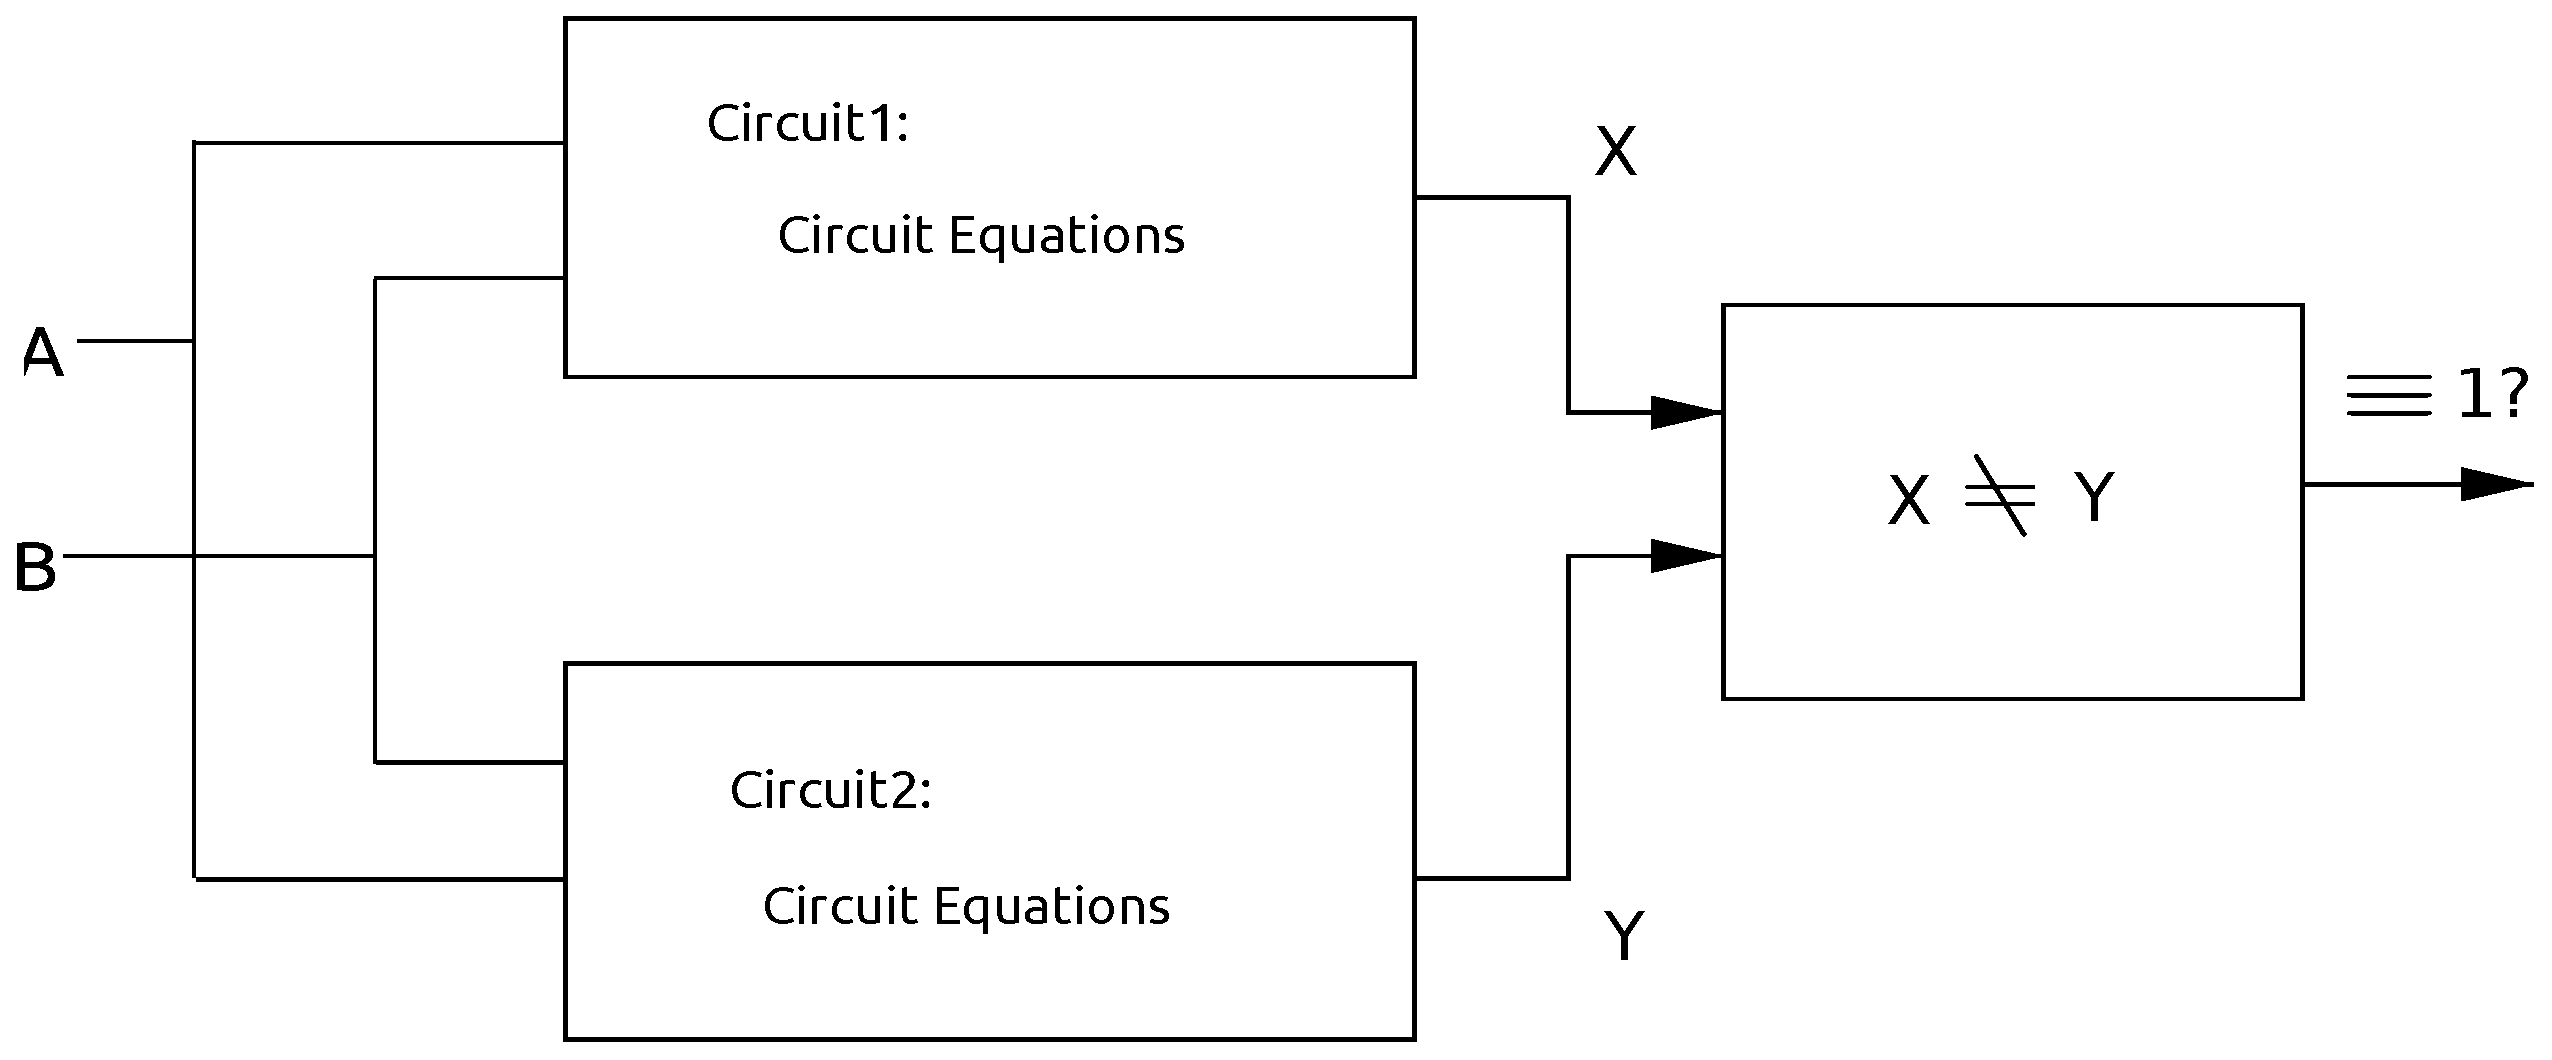
\includegraphics[scale=0.3]{./figures/miter.eps}
}
\caption{The equivalence checking setup: miter.}
\label{fig:miter}
\end{figure}

The equivalence verification setup is shown in Fig. \ref{fig:miter}. 
Given circuits $C_{1}$ and $C_{2}$, 
we want to prove that for all possible inputs, 
the output $X$ of circuit $C_{1}$ is always equal to the output $Y$ of circuit $C_{2}$ . 
This can be, conversely, modeled as proving that $X \neq Y$ has no
solutions. Such a setup is called a ``miter'' circuit, and proving
infeasibility of the miter is a standard practice in combinational
circuit verification. This is mostly because it enables the use of
{\it constraint-solvers} (such as SAT solvers) to prove/disprove
equivalence.  

The constraints for circuits $C_1$ and $C_2$ are modeled as
polynomials over $\mathbb{F}_{2^k}$ using Equations \ref{b2poly}. 
The $X\neq Y$ constraint corresponding to the miter is also modeled as
a polynomial in $\mathbb{F}_{2^k}$ as follows:
\begin{equation}
t(X - Y) = 1, \text{where $t$ is a free variable in }\mathbb{F}_{2^k}  
\end{equation}
The correctness of the above
constraint modeling can be shown as follows: 
\begin{itemize}
	\item When $X = Y, X-Y =0$, so $t\cdot 0 = 1$ has no
          solutions, and the miter is infeasible.
	\item When $X\neq Y, (X-Y) \neq 0$. Over any field, every
          non-zero element has a multiplicative inverse. Let $t^{-1} =
          (X-Y)$. Then $t \cdot t^{-1} = 1$ will always have a
          solution over $\mathbb{F}_{2^k}$. 
\end{itemize} 
% If indeed there are no solutions to $X \neq Y$, then it
% implies that $X$ is always equal to $Y$. Otherwise, 
% if there is a solution to our problem instance, then there is an assignment where
% $X$ differs from $Y$ which indicates a bug in the circuit.   

The above $t(X-Y) = 1$ model for the miter can also be employed over 
$\mathbb{F}_{2}$, i.e. the Boolean ring. Since $1$ is the only
non-zero element in $\mathbb{F}_{2}, t = 1$, and the $X\neq Y$
constraint is specified as $X+Y+1 = 0 \pmod 2$.	  
%\item As a special case over $\mathbb{F}_2$, 

%Following the mapping rules given in Equations \ref{b2poly}, 
%the circuit equations are transformed into polynomial representation.

Overall, the entire miter circuit can be modeled as a polynomial system over
$\mathbb{F}_{2^k}$: 

\begin{eqnarray}\label{eqn:miterbit}
 \left .  \begin{aligned}
f_1^{1}(x_1,x_2,\cdots, x_d)  \\
\vdots  \\
f_A: A + a_0 +  a_1 \alpha + \dots + a_{k-1}\alpha^{k-1}\\
f_{X}: X+x_{0}+x_{1}\cdot \alpha+\dots+ x_{k-1}\cdot \alpha^{k-1} \\
%f_{Z}: Z+z_{0}+z_{1}\cdot \alpha,\cdots,{z_{k-1}}\cdot \alpha^{k-1}=0   
 \end{aligned} 
\ \right\}
 &\qquad&  \text{\it Circuit $1$} \nonumber \\
 \left . \begin{aligned}
f_1^{2}(x_1,x_2,\cdots, x_d)=0  \\
\vdots  \\
f_B: B + b_0 +  b_1 \alpha + \dots + b_{k-1}\alpha^{k-1}\\
f_{Y}: Y+y_{0}+y_{1}\cdot \alpha+\dots+ y_{k-1}\cdot \alpha^{k-1} \\
 \end{aligned} 
\right\}
 &\qquad&  \text{\it  Circuit $2$}  \\
 \left .  \begin{aligned}
f_{m}:t\cdot (X-Y)+1=0  \nonumber 
 \end{aligned} 
\right\}
 &\qquad& \text{Miter:}X \neq Y \nonumber 
\end{eqnarray}

Subsequently, we need to check whether or not there are any solutions
to the set of polynomials in Equations \ref{eqn:miterbit}. The
following example illustrates our polynomial system 
modeling. 

\begin{Example}\label{exp:miter}
Consider two functionally equivalent circuits 
%implementing $2$-bit adder 
over $\mathbb{F}_{2^2}$. The miter is shown in Figure
\ref{fig:2bitadder}. 
	\begin{figure}[htb]
		\centerline{
		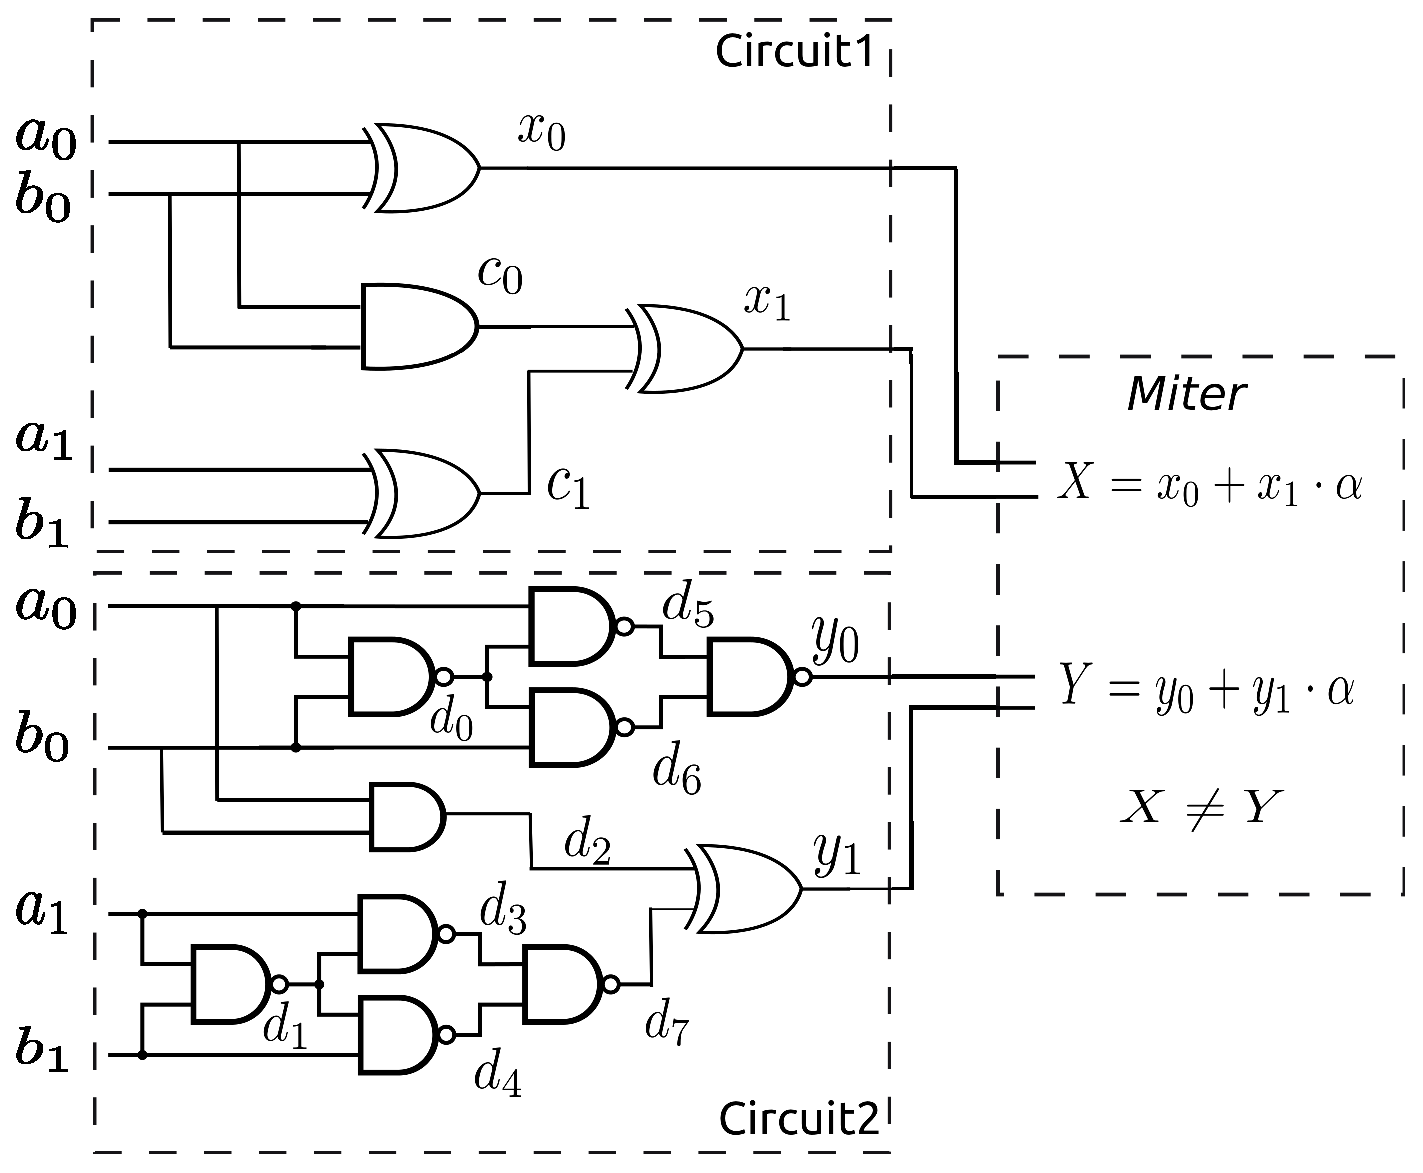
\includegraphics[scale=0.35]{./figures/2bitadder.eps}
		}
		\caption{Miter for $2$-bit circuit equivalence.}
		\label{fig:2bitadder}
	\end{figure}

%Then the miter circuit described in Figure \ref{fig:2bitadder} is
The miter is modeled as a system of polynomials, where the outputs of
$C_1, C_2$ are expressed at word level as: $X+x_{0}+x_{1}\cdot \alpha$ and
$Y+y_{0}+y_{1}\cdot \alpha$. 

\begin{eqnarray}%[htb]
 \left .  \begin{aligned}
	x_0&=a_0 \oplus b_0  \Rightarrow x_0+a_0 + b_0 \\
	c_0&=a_0\wedge b_0   \Rightarrow c_0+a_0 \cdot b_0\\
	c_1&=a_0\oplus b_1   \Rightarrow c_1+a_0 + b_1 \\
	x_{1}&=c_{0}\oplus c_{1}  \Rightarrow x_{1}+c_{0}+ c_{1} \\
	&X+x_{0}+x_{1}\cdot \alpha				\\
	 \end{aligned} 
\ \right\}
 &\qquad&  \text{\it Circuit $1$} \nonumber \\
 \left . \begin{aligned}
d_{0}&=\neg (a_{0} \wedge b_{0}) \Rightarrow d_{0}+ a_{0} \cdot b_{0}+1  \\
	d_{1}&=\neg (a_{1} \wedge b_{1}) \Rightarrow d_{1}+ a_{1} \cdot b_{1}+1  \\
	d_{2}&= a_{0} \wedge b_{0} \Rightarrow d_{2}+ a_{0}\cdot b_{0} \\
	d_{3}&=\neg (a_{1} \wedge d_{1}) \Rightarrow d_{3}+ a_{1} \cdot d_{1}+1  \\
	d_{4}&=\neg (b_{1} \wedge d_{1}) \Rightarrow d_{4}+ b_{1} \cdot d_{1}+1  \\
	d_{5}&=\neg (a_{0} \wedge d_{0}) \Rightarrow d_{5}+ a_{0} \cdot d_{0}+1  \\
	d_{6}&=\neg (b_{0} \wedge d_{0}) \Rightarrow d_{6}+ b_{0} \cdot d_{0}+1  \\
	d_{7}&=\neg (d_{3} \wedge d_{4}) \Rightarrow d_{7}+ d_{3} \cdot d_{4}+1  \\ 
	y_{0}&=\neg (d_{5} \wedge d_{6}) \Rightarrow y_{0}+ d_{5} \cdot d_{6}+1  \\
	y_{1}&=d_{2} \oplus d_{7}   \Rightarrow  y_{1}+d_{2} + d_{7}	\\
	&Y+y_{0}+y_{1}\cdot \alpha				\\
 \end{aligned} 
\right\}
 &\qquad&  \text{\it  Circuit $2$} \nonumber \\
 \left .  \begin{aligned}
	&t\cdot (X-Y)+1=0 				
 \end{aligned} 
\right\}
 &\qquad& \text{Miter:}X \neq Y
\end{eqnarray}

\end{Example}


With the polynomial model given above, we formulate our problem as a {\bf Weak Nullstellensatz} problem, 
which is described next.

%%%%%%%%%%%%%%%%%%%%%%%%%%%%%%%%%%%%%%%%%%%%%%%%%%%%%%%%%%%%%%%%
%%%%%%%%%%%%%%%%%%%%%%%%%%%%%%%%%%%%%%%%%%%%%%%%%%%%%%%%%%%%%%%%
%%%%%%%%%%%%%%%%%%%%%%%%%%%%%%%%%%%%%%%%%%%%%%%%%%%%%%%%%%%%%%%%
\subsection{Verification Problem Formulation as Weak Nullstellensatz}

As described in Equation \ref{eqn:miterbit} and Example \ref{exp:miter},
to formulate our verification test, we first analyze the miter circuit and 
model the Boolean gate-level operators as polynomials over $\mathbb{F}_2$
-- i.e. two sets of implementation polynomials representing $C_{1}$ and $C_{2}$, 
and the miter polynomials: $X \neq Y$ ($X,Y$ are outputs of $C_{1}$ and $C_{2}$). 
Subsequently, we can reason whether or not solutions exist
to this polynomial system. 

For this purpose, we wish to use techniques from computer algebra and
algebraic geometry to reason about the solutions (variety) to the
polynomial equations (ideal).  

{\bf {Notation:}} Let $F_1, F_2$ represent the set of
polynomials 
generated from circuit $C_1$ and 
$C_2$, respectively. Let $f_m$ represent the miter polynomial. Let
$F=\{F_1,F_2,f_m\}=\{f_1,f_2,\ldots,f_s, f_m\}$ denote this set of
polynomials derived from the miter circuit.  Let $\{x_1,\dots,x_d\}$
denote all variables occurring in $F$. Let $J = \langle
F_1,F_2, f_m\rangle \subset \mathbb{F}_{2^k}[x_{1},\dots,x_{d}]$
denote the ideal generated by these polynomials. 
Subsequently, $V_{\mathbb{F}_{2^k}}(J)$ denotes the variety
(solutions) of $J$ over $\mathbb{F}_{2^k}$. 

Our verification problem
can be formulated as the evaluation: 
\begin{equation}
V_{\mathbb{F}_{2^k}}(J)=\emptyset?
\end{equation}
%To solve this problem, A direct answer is {\bf Weak Nullstellensatz} 


{\it Weak  Nullstellensatz} \cite{null:1890} explicitly specifies the
condition when a variety is empty. 

%%%%%%%%%%%%%%%%weak nullstellensatz%%%%%%%%%%%%%
\begin{Theorem}
$\left[\bf{Weak\  Nullstellensatz}\right]$ Let $J \subset \overline
{\mathbb{K}}[x_1, x_2, \cdots, x_d]$ be an ideal satisfying
$V_{\overline{\mathbb{K}}}(J)=\emptyset$. Then $I=\overline {\mathbb{K}}[x_1,
x_2, \cdots, x_n] \iff \{1\} \in J$. 
\end{Theorem}

Recall that a reduced Gr\"obner basis is a canonical representation of
an ideal.  We know that the unit ideal $\langle 1 \rangle$ can 
generate the entire set of polynomials in $\overline{\mathbb{K}}[x_1,
x_2, \cdots, x_n]$.  Therefore, Weak Nullstellensatz can be further
described via Gr\"obner basis as:

\begin{Corollary}\label{cor:wnf2}
$\left[\bf{Weak\  Nullstellensatz}\right]$ Let $I \subset \overline
{\mathbb{K}}[x_1, x_2, \cdots, x_d]$ be an ideal satisfying
$V(I)=\emptyset$.  Then the Reduced Gr\"obnerBasis(I)$=\{1\}$.
\end{Corollary}

The {\it Weak Nullstellensatz} now offers us a way to evaluate whether
the system of multivariate polynomial equations has a common solution
in ${\overline {\mathbb{K}}}^d$. 

However, {\it Weak Nullstellensatz} is stated over an algebraically
closed field $\overline{\mathbb{K}}$.
Our problem is modeled over $\mathbb{F}_{2^{k}}$ which is not 
algebraically closed. Therefore, {\it Weak Nullstellensatz} is bound
to fail when applied directly, without modification, to finite fields. 

Let us explain why {\it Weak Nullstellensatz} fails when applying to
the field $\mathbb{F}_{2}\subset \mathbb{F}_{2^{k}}$ by an example. 
\begin{Example} \label{exp:wnfail}
We are given an implementation of a circuit over $\mathbb{F}_2 \subset \mathbb{F}_{2^{k}}$: 
\begin{equation}
x_1=a \vee (\neg a \wedge b)
\end{equation}
Its corresponding specification is :
\begin{equation}
y_1=a \vee b
\end{equation}
where $x_1$ and $y_1$ are symbolically different but functionally equivalent.  
Then we transform the circuit equations into their polynomial forms:
\begin{eqnarray}
x_1=a \vee (\neg a \wedge b) &\mapsto& x_1 + a + b\cdot (a+1) + a\cdot b \cdot (a+1) \pmod 2 \nonumber \\
y_1=a \vee b  &\mapsto& y_{1}+a+b+a\cdot b \pmod 2 \nonumber \\
x_1 \neq y_{1}  &\mapsto& x_1+y_1+1 \pmod 2 \nonumber
\end{eqnarray}
\end{Example}
Then the reduced Gr\"obner basis of above polynomials with term
ordering {\it lex} $x_{1}>y_{1}>a>b$ is:  
\begin{eqnarray}
a^{2}\cdot b+a \cdot b+1 \nonumber \\
y_{1}+a \cdot b+a+b \nonumber \\
x_{1}+a \cdot b+a+b+1 \nonumber 
\end{eqnarray}

which is not equal to $\langle 1\rangle$, even though their variety is
empty. The reason for this can be explained as follows. 

\begin{figure}[htb]
\centerline{
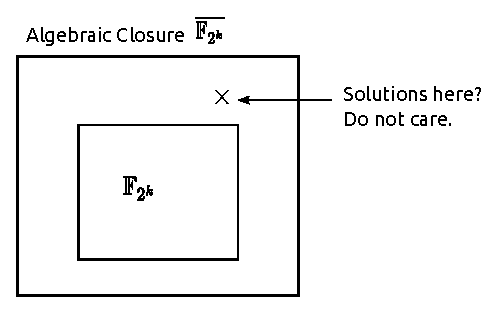
\includegraphics[scale=1]{./figures/closure.eps}
}
\caption{ A solution (bug) in
  $(\overline{\mathbb{F}_{2^{k}}}-\mathbb{F}_{2^k})$ is a ``don't
  care''.} 
\label{fig:closure}
\end{figure}

As shown in Figure \ref{fig:closure}, $\overline{ \mathbb{F}_{2^k} }$
is the algebraic closure of $\mathbb{F}_{2^k}$.
If there is no solution to ideal $J$ in the algebraic closure
$\overline{ \mathbb{F}_{2^k}}$,  then there is no solution in
$\mathbb{F}_{2^k}$ either. However, what happens when there is a
solution in $\overline{ \mathbb{F}_{2^k}}$, i.e. $1 \notin GB(J)$?  
In this case, it means that there is a {\it non-empty set of
  solutions} to the polynomial system in
$\overline{\mathbb{F}_{2^k}}^d$. There are two possibilities:  
\begin{itemize}
	\item The solution(s) may lie within $\mathbb{F}_{2^k}$.
	\item The solution(s) may lie in $\overline
          {\mathbb{F}_{2^k}}$, but outside $\mathbb{F}_{2^k}$, as
          depicted in  Figure \ref{fig:closure}. 
\end{itemize}
We are interested in finding out whether or not $X \neq Y$ over $\mathbb{F}_{2^{k}}$ 
-- i.e. whether the circuit has bugs over the given field
$\mathbb{F}_{2^{k}}$. We do not care if the solution is outside the
field $\mathbb{F}_{2^{k}}$, in which case the bug is really a ``don't
care'' condition (akin to a ``false negative'' in design verification
parlance).  


To address this problem, {\it Weak Nullstellensatz} needs to be suitably
modified for application over finite fields $\mathbb{F}_{2^{k}}$. 
%%%%%%%%%%%%%%%%weak nullstellensatz in finite field%%%%%%%%%%%%%
\begin{Theorem}\label{wnull:ff}
$[\bf{Weak~Nullstellensatz~in~\mathbb{F}_{2^k}}]$\\
Given $f_1,f_2,\cdots,f_s \in \mathbb{F}_{2^k}[x_1,x_2,\cdots,x_d]$. 
Let $J=\langle f_1,f_2,\cdots,f_s\rangle \subset \mathbb{F}_{2^k}[x_1,
x_2, \cdots, x_d]$ be an ideal. Let $J_0 = \langle 
x_1^{2^k}-x_1,x_2^{2^k}-x_2,\cdots,x_d^{2^k}-x_d \rangle$ be the ideal
of vanishing polynomials in $\mathbb{F}_{2^k}$. Then
$V_{\mathbb{F}_{2^k}}(J) = V_{\overline {\mathbb{F}_{2^k}}}(J +
J_0)=\emptyset$,  if and only if the reduced
Gr\"obnerBais$(J+J_{0})=\{1\}$. 
\end{Theorem}
 
\begin{Proof}
%For convenience, let $J_0$ denote $x_1^{2^k}-x_1,x_2^{2^k}-x_2,\cdots,x_d^{2^k}-x_d$.
According to the definition of vanishing polynomials over
$\mathbb{F}_{2^k}$, we have $V_{\overline
  {\mathbb{F}_{2^k}}}(J_0)={\mathbb{F}_{2^k}^d}$. 
From Lemma \ref{lem:closure}, we know:
\begin{equation}
	V_{\overline {\mathbb{F}_{2^k}}}(J+J_0)=V_{\mathbb{F}_{2^k}}(J). 
\end{equation}
Combining with Corollary \ref{cor:wnf2}, we conclude:
\begin{equation}
V_{\overline {\mathbb{F}_{2^k}}}(J+J_0)=\emptyset \Leftrightarrow
\text{ reduced Gr\"obnerBais}(J+J_0) =\{ 1\}
\end{equation}
% Therefore, 
% \begin{equation}
% V_{\overline {\mathbb{F}_{2^k}}}(J+J_0)=V_{\mathbb{F}_{2^k}}(J)=\emptyset \Leftrightarrow {\text{Reduced Gr\"obnerBais(J+$J_{0}$)}}=\{ 1\}  \nonumber
% \end{equation}
%{}
\end{Proof}

\begin{Example}
Re-visiting Example \ref{exp:wnfail}, we need to append the vanishing
polynomials $a^2-a,b^2-b,x_1^2-x_1,y_1^2-y_1$ to given ideal.  Now
when we compute the reduced Gr\"obner basis, we get: reduced-GB$(x_1+
a + b\cdot(a+1) + a\cdot b\cdot(a+1),y_1+a+b+a\cdot
b,x_1+y_1+1,a^2-a,b^2-b,x_1^2-x_1,y_1^2-y_1)=\{1\}$ which proves
$x_1=y_1$. 
\end{Example}


{\bf Verification Problem Formulation:}
Through Weak Nullstellensatz over $\mathbb{F}_{{2^k}}$, given an ideal
$J \in \mathbb{F}_{2^k}[x_{1},\dots,x_{d}]$,  we can determine whether
the variety of $J$ is empty by analyzing the corresponding reduced
Gr\"obner basis of $J+J_0$. 

For our verification problem, we take the polynomials $\{F_1, F_2,
f_m\} = \{f_1, \dots, f_s, f_m\}$  representing the miter circuit
constraints to generate ideal $J$. Then we append the vanishing
polynomials $\{x_1^{2^k} - x_1, \dots, x_d^{2^k} - x_d\}$ of ideal
$J_0$. We compute the reduced Gr\"{o}bner basis $G$ of $J+J_0$ and
check if $G$ equals to the unit ideal $\{1\}$. The two circuits are
functionally equivalent if and only if $G = \{1\}$.

The critical issue in the Weak Nullstellensatz formulation is the
computational complexity of a Gr\"obner basis (as given in
Theorem \ref{thm:gb-complexity}). 
To overcome this complexity, we again wish to exploit our
circuit topology-based term ordering from Proposition
\ref{prop:top-order} for polynomial representation.  
Note that according to the term ordering from Proposition
\ref{prop:top-order}, the set of polynomials in $\{F_1,F_2\}$ does
constitute a Gr\"obner basis -- as $C_1$ and $C_2$ are independent
circuits. However, with the miter polynomial $f_m$, the set of
polynomials $F = \{F_1, F_2, f_m\}$ 
%corresponding to the miter  circuit (verification instance) 
does not constitute a Gr\"obner basis. This is because there always
exists one polynomial $f_o \in F, (f_o \neq f_m)$ corresponding to the 
output of either $C_1$ or $C_2$ with a leading term that is not
relatively prime w.r.t. the leading term of the miter polynomial
$f_m$. Their corresponding S-polynomial computation also does not
reduce to zero. This is shown in Example \ref{exp:1bitmiter}.   

%\begin{Example}\label{exp:1bitmiter}
	
%\begin{figure}[hbt]
%\centerline{
%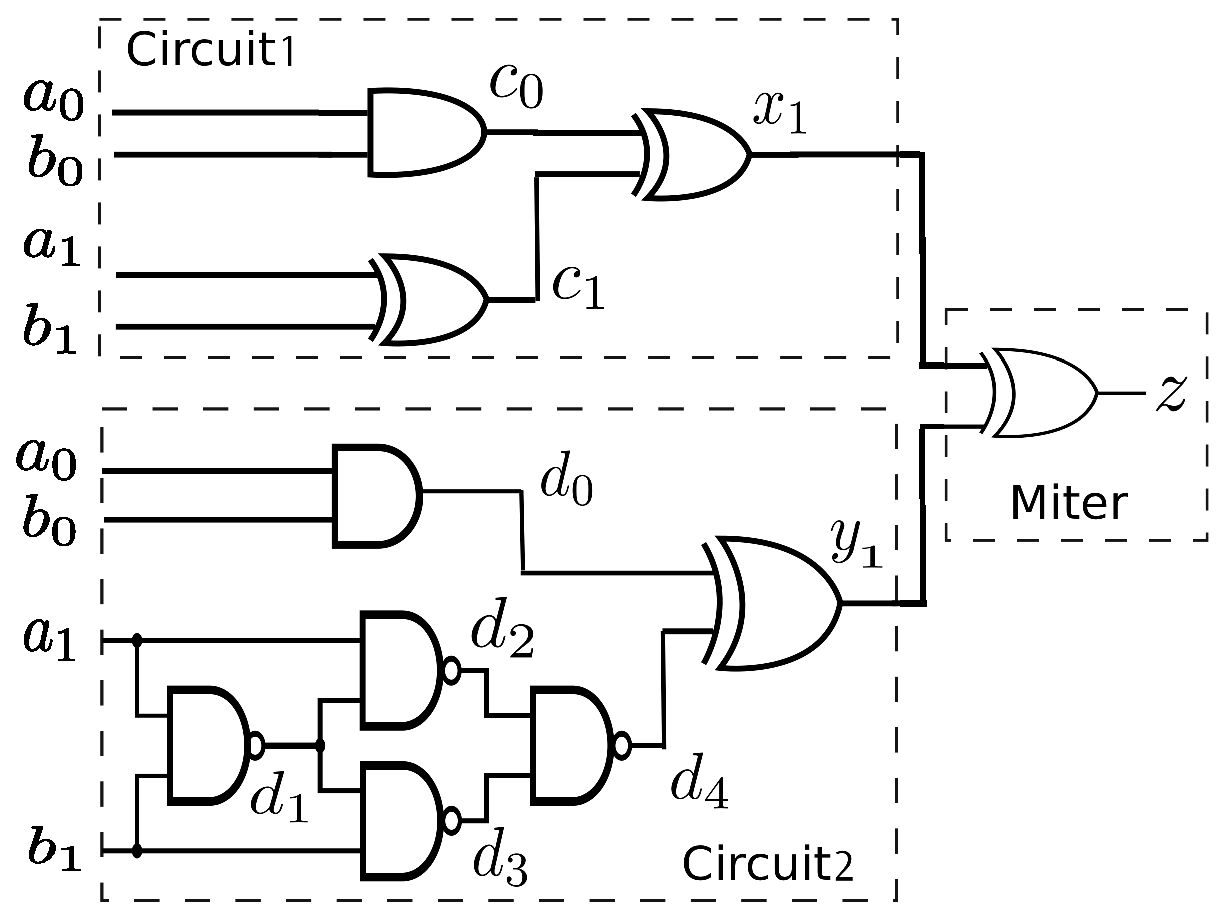
\includegraphics[scale=0.40]{./figures/1bitmiter.eps}
%}
%\caption{Miter}
%\label{fig:1bitmiter}
%\end{figure}

%The above two circuits are functiaonally equivalent and their polynomials are described as follows:


%\begin{eqnarray}
 %\left .  \begin{aligned}
	%& c_0 + a_0\cdot b_0   \\
	%& c_1 + a_1 + b_1   \\
	%& x_1 + c_0 + c_1   \\
	 %\end{aligned} 
%\ \right\}
 %&\qquad&  \text{\it Circuit $1$: $F_{1}$} \nonumber \\
 %\left . \begin{aligned}
	%&d_0+a_0 \cdot b_0 \\
	%&d_1+a_1\cdot b_1+1   \\
	%&d_2+ a_1\cdot d_1+1   \\
	%&d_3+ b_1\cdot d_1+1  \\
	%&d_4+d_2\cdot d_3			\\
	%&y_1+d_0+ d_4   		\\
 %\end{aligned} 
%\right\}
 %&\qquad&  \text{\it  Circuit $2$}: F_{2}  \\
 %\left .  \begin{aligned}
	%& x_1 + y_1 + 1  			
 %\end{aligned} 
%\right\}
 %&\qquad& \text{Miter $f_{m}$:}X \neq Y \nonumber
%\end{eqnarray}

\begin{Example}\label{exp:1bitmiter}
Let us re-consider Example \ref{exp:wnfail}. Based on our topological
term ordering of the circuit, we impose a {\it lex} term order with: \\  
$ x_1 >  y_1 > d_4 > d_3 > d_2 > d_1> d_0 >c_1 > c_0 > a_0 > a_1 > b_0 > b_1$, \\ 
Then the set of polynomials of the miter circuit
$\{ F_{1},F_{2}, f_{m} \}$ does not constitutes a Gr\"obner
Basis. This is because the miter polynomial $f_m: t X - t Y+1$
and output polynomial $f_X$ of circuit $C_1$, $f_X: X+x_0+x_1\cdot
\alpha$, has a common variable $X$  in their leading terms $tX$
and $X$, respectively. Therefore, $lt(f_m)$ and $lt(f_o)$ are not
relatively prime. Moreover, $Spoly(f_m,f_X)$ $\stackrel{F_1, F_2,
  f_m}{\longrightarrow} r$, $r\neq 0$, thus violating the property of
a Gr\"obner basis that all S-polynomials should reduce to zero. 
\end{Example}

This suggests that we may have to compute a reduced Gr\"obner
basis. However, in the next section, we describe our results that can
identify {\it a minimum number of S-polynomial computations} that are
sufficient and necessary to prove equivalence or to detect bugs. 

%%%%%%%%%%%%%%%%%%%%%%%%%%%%%%%%%%%%%%%%%%%%%%%%%%%%%%%%%%%%%%%%%%%%
%%%%%%%%%%%%%%%%%%%%%%%%%%%%%%%%%%%%%%%%%%%%%%%%%%%%%%%%%%%%%%%%%%%%
%%%%%%%%%%%%%%%%%%%%%%%%%%%%%%%%%%%%%%%%%%%%%%%%%%%%%%%%%%%%%%%%%%%%
\section{Verification Uusing a Minimum Number of S-polynomial Computations}


% Let $F_1, F_2$ represent polynomials generated from circuit $C_1$ and
% $C2$ respectively. Let $f_m$ represent the miter polynomial.
% Let $F=\{F_1,F_2,f_m\}=\{f_1,f_2,\ldots,f_s, f_m\}$ denote this set of
% polynomials derived from the miter circuit.  Let $\{x_1,\dots,x_d\}$
% denote all variables occurring in $F$. Let $J = \langle
% F_1,F_2,f_m\rangle \subset \mathbb{F}_{2^k}[x_{1},\dots,x_{d}]$ denote
% the ideal generated by these polynomials. Let $f_o \in F$ denote the
% only polynomial such that $lt(f_o)$ and $lt(f_m)$ are not relatively
% prime.  

% Based on our term order, such polynomials $f_o, f_m \in F$ always
% exist. Polynomial $f_o \neq f_m$ corresponds to the output of circuit
% $C1$ or $C_2$. Moreover, the leading term of miter polynomial $f_{m}$
% always corresponds to the output of either circuit $C_1$ or $C2$. 
% Let $T=\{x_1,\dots,x_d\}$ denote all variables occurring in $F$, of
% which, let $T_{PI} \subset T$ denote the set of primary inputs. 

% To derive a minimum number of S-polynomial computations for our
% problem,  we first consider a pair of polynomials that are not
% relatively prime: $f_{m}$ and $f_{o}$. In Example \ref{exp:wnfail},
% $f_o=X+x_0+x_1\cdot \alpha$ and $f_m=t\cdot X-t\cdot Y+1$.  Because of
% the existence of $f_{m}$ and $f_{o}$, $\{F_1,F_2,f_m\}$ does not
% constitute a Gr\"obner basis.  


% Therefore, to claim that $f_{m}$ and $f_{o}$ is the only pair of polynomials that needs to be reduced in Gr\"obner basis computation
% of $\{ F \}$, we have the following lemma and theorem: 

To identify a minimum number of S-polynomial computations in
Buchberger's algorithm, we make use of the following lemma. 
\begin{Lemma}\label{lem:root2}
Let $r \in \mathbb{F}_2[x_1, \dots, x_d]$ be a multi-linear polynomial
expression; i.e. r is a nonconstant polynomial such that every
monomial term in $r$ contains variables of degree $1$. Then $r$ has a
root in $\mathbb{F}_2^d$. 
\end{Lemma}

\begin{Proof}
Let $l(r)$ denote the number of nonzero monomials appearing in $r$. We
will perform induction on $l(r)$. Note that in $\mathbb{F}_2$,
the coefficient of all non-zero monomials is 1.

The case $l(r)=1$ is trivial, as $r = x_1x_2\dots x_t$, for some $t
\leq d$. A polynomial with one monomial term always has a solution. 

For the general case, $l(r) \geq 2$. Then  we can always write $r =
r' + M$ where $M$ is a product of monomials. After appropriately
re-labeling the variables, we can assume that $x_1$ divides $M$,
i.e. $x_1$ appears in $M$. If $x_1$ divides $r'$ too, then $x_1$
divides $r$ as well. As a consequence, we obtain $x_1=0$ as a
solution for $r=0$. So, $r$ has a root in $\mathbb{F}_2$. 

If $x_1$ does not divide $r$, then it does not divide $r'$. So
variable $x_1$ does not appear in $r'$. Then, let $r"=\mathcal{F}(0,
x_2,\ldots, x_d)$. Note that $l(r") < l(r)$, as monomial $M$ does not
appear in $r"$. By induction, there is a solution $(x_2, \dots, x_d)$
for $r"=0$, which also gives a solution $(0, x_2, \ldots, x_d)$ for
$r$.  Thus $r$ always has a root in $F_2$.
\end{Proof}

Now we state and prove the following theorem.

\begin{Theorem}\label{thm:miter}
Let $F_1, F_2$ correspond to the set of polynomials
derived from circuits $C_1, C_2$, respectively. Let $f_m$ be the miter
polynomial. Let $F = \{F_1, F_2, f_m\}$ and $J=\langle F \rangle
\subset \mathbb{F}_{2^k}[x_{1},\dots,x_{d}]$ be the ideal of
polynomials corresponding to the miter circuit. Impose the circuit
topology-based monomial order $>$ from Proposition
\ref{prop:top-order}. Let $F_0 = \{ x_1^{2^k} - x_1, \dots,
x_d^{2^k} - x_d\}$ be the vanishing polynomials of $\mathbb{F}_{2^k}$;
and $J_0 = \langle F_0 \rangle$. Let $f_o \in F$ ($f_o \neq f_m$)
be the only polynomial such that  the leading terms of $f_m, f_o$ are
not relatively prime. Then $V_{\mathbb{F}_{2^k}}(J)=\emptyset \iff
r=1$, where $r$ is computed as  $Spoly(f_m, f_o)$
$\stackrel{F,F_0}{\longrightarrow}_+ r$. 

\end{Theorem}

\begin{Proof}
Let $q=2^k$, and let $G$ and $G_{red}$, respectively, denote the
Gr\"obner basis and the reduced Gr\"obner basis of $(J + J_0)$. Let
$T$ represent the set of all variables  occurring in $F$, and let
$T_{pi} \subset T$ denote the set of all primary inputs.   

Our objective is to deduce whether or not the variety
$V_{\mathbb{F}_{2^k}}(J)=\emptyset$, {\it without actually computing a
reduced Gr\"obner basis}. Recall, according to Theorem \ref{wnull:ff}, 
$V_{\mathbb{F}_{q}}(J)=\emptyset \iff G_{red}=\{1\}$, so we
only need to check whether $G_{red} =\{1\}$? Based on our term
ordering, we will try to identify the polynomials that constitute
$G_{red}$. 

% We claim that $GB(J+J_{0})=\{F,F_{0},r\}$, where $r$ is given
% above. In other words, $r$ is the only polynomial that will be
% generated in Buchberger's algorithm.

%This can be shown as follows: 
In the first iteration of Buchberger's
algorithm, $Spoly(f_m,f_o)$ is the only polynomial that needs to be
computed and reduced to obtain $r$, as all other S-polynomials reduce
to zero, due to Theorem \ref{thm:contrib}. We need to consider three
cases: 

\begin{itemize}
\item Case 1: $r = 1$.
\item Case 2: $r = 0$.
\item Case 3: $r$ is a  non-constant multi-linear polynomial
  consisting of only primary input variables of the circuit.
\end{itemize}

{\bf Case 1} is the trivial case: If $r = 1$, then $1\in G$, so
$G_{red} = \{1\}$ and therefore $V(J + J_0) = \emptyset$. The
miter is infeasible and the circuits are equivalent.

{\bf Case 2}: When $r = 0$, no new polynomial is created in
Buchberger's algorithm. Therefore $G = \{F, F_0\}$.
While the set $\{F, F_0\}$ is itself a Gr\"obner basis, it is not
reduced. So, what is the reduced basis $G_{red}$? We will show that
$G_{red} \neq \{1\}$ and this will imply that $V(J + J_0) \neq
\emptyset$.  

To reduce a Gr\"obner basis $G$, we take all polynomials $f \in G$ and
reduce $f\stackrel{G - f}{\longrightarrow}_+ f'$. All such $f'$
constitute $G_{red}$. We will consider such a reduction for $G = \{F,
F_0\}$. For all $f_j \in F$, let $f_j = x_j +P_j$, where 
$P_j = \text{tail}(f_j)$ and $lm(f_j)=x_j$ where $x_j \notin
T_{pi}$. This is due to our term order where only gate outputs ($x_j$)
appear as leading terms of all polynomials. Let $v$ be any variable
in $P_j$. If $v\in \{T-T_{pi}\}$ (non-primary-input), then $v=lm(f_k)$ 
($k\neq j$).  Thus $f_j \xrightarrow{ \{F,F_0\}-f_j }{f_j^{'}}$, where
$f_j^{'}=x_j+P_j^{'}$.  In such a case, $P_j^{'}$ contains only
primary inputs.  From a circuit-structure perspective,
this reflects that any internal gate output $x_j$ can be expressed in
terms of primary inputs.

Similarly, $x_i^{q}-x_i$ with $x_i\in \{T-T_{pi}\}$
will reduce to zero, and only vanishing polynomials of primary inputs
will remain in $F_0$. Moreover, since circuit inputs are bit-level,
$x_{pi}^2 = x_{pi}$; so $x_{pi}^{2}-x_{pi}$, $x_{pi}\in \{T_{pi}\}$,
are the vanishing polynomials remaining in the reduced basis. Let
$F^{'}=\{x_j+P_j^{'}\}$, where $x_j \in T$. Then, the reduced
Gr\"obner basis $G_{red}$ of $\{F, F_0\}$ = $reducedGB(\{F\} \cup
\{x_i^{q}-x_i\})=\{F^{'}\} \cup \{x_{pi}^{2}-x_{pi}\}$. Clearly,
$G_{red} \neq 1$. We conclude, if $r=0$, $G_{red} \neq \{1\}$, and
$V(J + J_0) \neq \emptyset$. The miter constraints are feasible and the
circuits are not equivalent. 


{\bf Case 3}: If $r$ is a non-constant polynomial, then due to our
term order and Corollary \ref{thm:mini}, $r$ will contain only the
primary input variables of the circuit. Moreover, as these variables
are Boolean, $x_{pi}^2 = x_{pi}^3 = \dots = x_{pi}$, all variables in
the monomials of $r$ have degree 1, and $r$ is multi-linear.

% In such a case, according to
% the proof in Theorem \ref{thm:contrib}, $Spoly(r,x_{pi}^{q}-x_{pi})
% \stackrel{G}\rightarrow _+0$, where $x_{pi}$ is a primary
% input. Therefore, for both cases in Step 1, 
% there are no new polynomials generated.

% With the knowledge of $GB(J+J_{0})=\{J,J_{0},r\}$, we can deduce what
% the $redGB(J+J_{0})$ is now. 


%The last case is when $r \neq 0$, what is $redGB(J+J_{0})$? 

%Recall that $lm(r)$ can merely contain primary inputs and is a
%multi-linear polynomial.  
After the first iteration of Buchberger's algorithm, we obtain $\{F,
F_0, r\}$ in the basis. Because $r$ contains only primary inputs,
$lt(r)$ is relatively prime w.r.t. leading terms of all polynomials in
$F$. So the Gr\"obner basis of $\{F,r\}$ is $\{F,r\}$ itself.

However, $\{F,r\}\cup \{F_{0}\}$ is {\it not} a Gr\"obner basis,
because $lm(r)$ and $lm(x_k^{q}-x_k)$ are not relatively prime when
$x_k\in T_{pi}$.  Therefore, $G = GB(\{F,r\}\cup
\{F_{0}\}) = \{F\} \cup GB(r\cup \{F_{0}\})$. In such a
case, if we can show that $1 \notin GB(r\cup \{F_{0}\})$, then
$1\notin GB(\{F,F_{0},r\})$. 

To show $1 \notin GB(r\cup \{F_{0}\})$, we utilize the Weak
Nullstellensatz Theorem \ref{wnull:ff}: if $V(r\cup \{F_{0}\})\neq
\emptyset$,  then $1 \notin GB(r\cup \{F_{0}\})$. In Lemma
\ref{lem:root2}, we showed that if $r$ is a multi-linear  
polynomial, it always has a root. This means that $V(r\cup
\{F_{0}\})\neq \emptyset$.  Therefore $1 \notin GB(r\cup
\{F_{0}\})$. This proves Case 3: if $r$ is not 0 or 1, then $\{1\}
\notin G = GB(F,F_0)$.  

So, we conclude that:
\begin{equation}
	V_{\mathbb{F}_{2^k}}(J)=\emptyset \iff r=1.
\end{equation}
\end{Proof}

Combining with Corollary \ref{thm:mini}, the above theorem can be
re-stated based on a minimum Gr\"obner basis. 
\begin{Corollary}\label{cor:miter}
Let $J=\langle F \rangle \subset \mathbb{F}_{2^k}[x_{1},\dots,x_{d}]$ 
on which we impose our circuit-based monomial order $>$.
Let $J_0^{PI}=\langle x_{pi}^{2}-x_{pi}\rangle$, where $x_{pi}\in PI$.
Let $f_o, f_m$ be the only polynomial pair such that $lm(f_m),
lm(f_o)$ are not relatively prime. Then
$V_{\mathbb{F}_{2^k}}(J)=\emptyset \iff r=1$, where $r$ is computed as
$Spoly(f_m,f_o) \stackrel{J,J_0^{PI}}{\longrightarrow}_+ r$.

\end{Corollary}

Theorem \ref{thm:miter} and Corollary \ref{cor:miter} provide the
foundation of our verification formulation. We only need one
S-polynomial computation to identify whether or not the two circuits
are equivalent. Our overall approach is described in the following
algorithm. 


\begin{algorithm}[hbt]
\SetAlgoNoLine

 \KwIn{Two Circuit Implementations with outputs $X$ and $Y$ (Boolean equations).}
 \KwOut{$1$ if $X=Y$. Bug polynomial $r$ if $X\neq Y$.}
%%%%%%%%%%%%%%%%%%%%
%%%%%%%%%%%%%%%%%%%%

\For { (i=0; i $<$ number of eqns; i++) }
  	{
  		\CommentSty{/*Each equation is transformed to polynomials */\;}
  		poly[i] = Eqn-to-Poly(eqn[i])\;
  		\CommentSty{/*Each equation is transformed to sum-of-term*/\;}
  		newpoly[i] = Sum-of-term(poly[i])\;
	}
%%%%%%%%%%%%%%%%%%%%
\CommentSty{/*Obtain circuit-based variable order*/\;}
ordered\_var=T\_Traversal(newpoly)\;
%%%%%%%%%%%%%%%%%%%%
\For {x $\in$ \{PI\} }
	{
		\CommentSty{/*append vanishing polynomials*/\;}
    	vanpoly[i]=$x^2+x$\;
	}    
\CommentSty{/*Identify polynomials that need to be reduced*/\;}	
{$f_{o}$, $f_{m}$}=Identify(newpoly, vanpoly)\;
To\_Be\_Reduced = Spoly($f_{o}$, $f_{m}$)\;
r=reduce(To\_Be\_Reduced, vanpoly, ordered\_var)\;
\eIf {r=\{1\}}
   {
   	 return $1$;
   }
   {
   	 return Bug polynomial $r$; %Bug polynomial;
   }	 

\caption{Our Proposed Equivalence Checking Algorithm}\label{alg:ecall}
\end{algorithm}


Algorithm \ref{alg:overall} first inputs the Boolean expressions of
the given circuit implementation. Each expression is then transformed
into polynomials $F$ using the mappings shown in Equation
\ref{b2poly}. All polynomials are then normalized into a sum-of-term
form using the distributive law $A(B+C)=AB+AC$.  
Then we perform a reverse topology traversal of the circuit to
derive our  variable and ordering. Then, we append vanishing
polynomials $F_{0} =\{x^2 + x \}$ for all $x \in$ primary inputs.  
Subsequently, we identify the two polynomials $f_{m}$ and $f_{o}$ that
have common variables in their leading terms. Finally, we conduct a
polynomial reduction of $Spoly(f_{m},f_{o})$  modulo $\{F \cup F_{0}\}$.  
If the reduction result is $r = 1$, the two circuits are equivalent. 
If $r \neq 1$, the circuits are not equivalent. Again, any assignment
to the variables that makes $r \neq 1$ provides an input vector that
can be used as a counter-example for debugging. 

%%%%%%%%%%%%%%%%%%%%%%%%%%%%%%%%%%%%%%%%%%%%%%%%%%%%%%%
%%%%%%%%%%%%%%%%%%%%%%%%%%%%%%%%%%%%%%%%%%%%%%%%%%%%%%%
%%%%%%%%%%%%%%%%%%%%%%%%%%%%%%%%%%%%%%%%%%%%%%%%%%%%%%%
\section{Improving Polynomial Division using $F_4$-style Reduction}

Through the results described above, the need for Buchberger's
algorithm is obviated and verification can be performed by analyzing
the result of just one S-polynomial reduction. Therefore, the most
intensive computational step is that of polynomial division 
$Spoly(f_m,f_o) \stackrel{F,F_0}{\longrightarrow}_+ r$. When the two
circuits $C_1, C_2$ are very large, the polynomial set $\{F, F_0\}$
also becomes extremely large. This division procedure then becomes the
bottleneck in verifying the equivalence. To further improve upon our 
approach, we exploit the relatively recent concept of $F_4$-style
polynomial reduction \cite{f4}, which implements polynomial division
using successive row-reductions on a matrix. 



% As described in Algorithm \ref{alg:overall}, polynomial reduction is
% the most time consuming step.  Therefore, to improve the efficiency of
% polynomial reduction,  polynomial reduction can be formulated as a
% matrix operation as used in $F4$ \cite{f4} that is a variant of
% Buchberger's algorithm.  In particular, polynomial reduction is
% formulated as row-reductions of a single matrix in $F4$. 

% However, the approach in \cite{f4} is applied for general purpose
% polynomial reduction and cannot achieve the best  performance for our
% problem.  Therefore, we need suitably engineer the $F4$-style
% reduction to better enhance our approach. 

Let us first describe the matrix representation for polynomial algebra
operations. 


{\bf Matrix representation of polynomials:} Each row $i$ of the matrix
$M$ corresponds to polynomial $f_i$, whereas each column $j$
corresponds to monomial $m_j$.
% of $f_i$corresponds to column $j$. 
If the $j^{th}$ entry on row $i$ in matrix is $1$, i.e. $M(i, j) = 1$,
it means the $j^{th}$ monomial is present in the $i^{th}$ polynomial.
Similarly, $M(i, j) = 0$ denotes the absence of $m_j$ in $f_i$. 
Since we are operating in $\mathbb{F}_{2^k}$, coefficients
are always $\{0, 1\}$, and no specific representation of coefficients
is required. Note, however, that the entries in rows and columns have
to satisfy the imposed term ordering. 
 
\begin{Example}
Given two polynomials: $f_{1}=a_{0}+a_{1}\cdot b_{1}+1$ and
$f_{2}=a_{0}\cdot b_{0}+b_{1}+1$ with term ordering {\it lex} with
$a_{0}>a_{1}>b_{0}>b_{1}$.  First, we sort all monomials occurring in
$f_{1}$ and $f_{2}$ w.r.t. term ordering: $a_{0}\cdot b_{0}
>a_{0}>a_{1}\cdot b_{1}> b_{1}>1$. 

Then, we associate these sorted monomials with the columns of the
matrix. The polynomials are also sorted according to the term order
before they are associated with the rows of the matrix. For example,
since $lm(f_{2})>lm(f_{1})$, $f_{2}$ appears on row $1$ and $f_{1}$
appears on row $2$. 
%(Actually $F4$ does not require such a polynomial ordering. 
The generated matrix is shown in Table \ref{tab:matrix}. 

	\begin{table}[t]
	\begin{center}
	\caption{Matrix representation for polynomials.}
	\label{tab:matrix}
	\begin{tabular}{|c|c|c|c|c|c|} \hline 
			&$a_{0}\cdot b_{0}$  	&$a_{0}$ 	&$a_{1}\cdot b_{1}$		&$b_{1}$ 	&$1$  \\
	\hline 
	$f_{2}$ & 1 &0 & 0 & 1 & 1 \\
	\hline
	$f_{1}$ & 0 &1 & 1 & 0 & 1 \\
	\hline
	\end{tabular}
	\end{center}
	\end{table}
\end{Example}	


Polynomial reduction requires operations of addition/subtraction and
cancellation of leading terms. We demonstrate how the
addition/subtraction and division operations are implemented on

{\bf Matrix subtraction for polynomials:} The subtraction of two
polynomials can be formulated as a row-eduction in the matrix. Since
coefficients of polynomials are computed (mod $2$) in our case,
row-reductions are also performed (mod $2$). 
%	which is another difference from $F4$-style reduction.
	
\begin{Example}	
	Again consider $f_{1}=a_{0}+a_{1}\cdot b_{1}+1$ and
        $f_{2}=a_{0}\cdot b_{0}+b_{1}+1$ with {\it lex} order:
        $a_{0}>a_{1}>b_{0}>b_{1}$. 
	Let us perform $f_{1}-f_{2}$: % the polynomial form is: 
	$f_{1}-f_{2}=f_{2}-f_{1} \pmod 2=a_{0}\cdot b_{0}+a_{0}+a_{1}\cdot b_{1}+b_{1}$.
	On the matrix, each entry on row $2$ is subtracted from %subtracts
        the corresponding entry on row $1$ and the result is stored in row
        $2$, as shown in Table \ref{tab:subtract}.
	
	 \begin{table}[b]
	\begin{center}
	\caption{Matrix subtraction of polynomials.}
	\label{tab:subtract}
	\begin{tabular}{|c|c|c|c|c|c|} \hline 
			& $a_{0}\cdot b_{0}$  & $a_{0}$ & $a_{1}\cdot b_{1}$ & $b_{1}$ & $1$  \\
	\hline 
	$f_{2}$ & 1 &0 & 0 & 1 & 1 \\
	\hline
	$f_2 - f_{1}$ & 1 &1 & 1 & 1 & 0 \\
	\hline
	\end{tabular}
	\end{center}
	\end{table}
	
\end{Example}

{\bf Matrix reduction for polynomials:} Polynomial
division is implemented as cancellation of leading terms. The
reduction step in Algorithm \ref{alg:polydiv} that cancels leading
terms is:   
\begin{equation}
\label{eqn:mat-red}
	{f_1}/{f_2}=f_{1}-\frac{lm(f_1)}{lm(f_2)}\cdot f_{2} 
\end{equation}
 
In matrix representation, 
%instead of creating two rows for $f_{1}$ and $f_{2}$, 
we create two rows, one each for $f_{1}$ and $\frac{lm(f_1)}{lm(f_2)}\cdot f_{2}$,
and then perform subtraction on the matrix; this is shown in Example
\ref{exp:division}.  
 
\begin{Example}\label{exp:division}
Given two polynomials: $f_{1}=a_{0}\cdot b_{1}+a_{0}+1$ and
$f_{2}=a_{0}+1$ with term order {\it lex}:
$a_{0}>a_{1}>b_{0}>b_{1}$. Consider the polynomial reduction:

\begin{equation}
{f_1}/{f_2}=f_{1}-\frac{a_{0}\cdot b_{1}}{a_{0}}\cdot f_{2} =f_{1}-b_{1}\cdot f_{2} \nonumber
\end{equation}
	 
We create two rows in matrix for $f_{1}$ and $b_{1}\cdot f_{2}$ and
insert monomials from $f_{1}$ and $b_{1}\cdot f_{2}$ into the matrix
columns, as shown in Table \ref{tab:red}.  
	 
	\begin{table}[t]
	\begin{center}
	\caption{Matrix reduction for polynomials: representation.}
	\label{tab:red}
	\begin{tabular}{|c|c|c|c|c|} \hline 
			&$a_{0} \cdot b_{1}$ & $a_{0}$ & $b_{1}$ & $1$  \\
	\hline 
	$b_{1}\cdot f_{2}$ & 1 &0 & 1  & 0 \\ 
	\hline
	$f_{1}$ & 1 &1 & 0 & 1  \\
	\hline
	\end{tabular}
	\end{center}
	\end{table}
	
	Then we conduct $f_{1}-b_{1}\cdot f_{2}$:
	
	\begin{table}[b]
	\begin{center}
	\caption{Matrix reduction for polynomials: subtraction.}
	\label{tab:red2}
	\begin{tabular}{|c|c|c|c|c|} \hline 
			&$a_{0} \cdot b_{1}$ & $a_{0}$ & $b_{1}$ & $1$  \\
	\hline 
	$b_{1}\cdot f_{2}$ & 1 &0 & 1  & 0 \\ 
	\hline
	$f_{1} - b f_2$ & 0 &1 & 1 & 1  \\
	\hline
	\end{tabular}
	\end{center}
	\end{table}
	
	Finally, row $2$ represents the reduction result of ${f_1}/{f_2}=a_{0}+b_{1}+1$.
	
 \end{Example}

With the above basic polynomial operations formulated as matrix
operations, we now describe our algorithm to create the matrix of
polynomials corresponding to our verification instance (miter
circuit). The algorithm is shown in Algorithm \ref{alg:matrix}. The
main idea behind this algorithm is to setup the rows  of
the matrix (polynomials) in a way that polynomial division can be
subsequently performed by subtracting row $i$ from row $i-1$. In the
algorithm, the computation $L:=L \cup \frac{mon}{lm(f_{k})}\cdot
f_{k}$ in the while-loop, actually corresponds to  
$\frac{lm(f_1)}{lm(f_2)}\cdot f_{2} $ in Equation \ref{eqn:mat-red}. 

\begin{algorithm}[hbt]
\SetAlgoNoLine

 \KwIn{$f, F=\{f_1,\dots,f_s$\} with $f_{1}>f_{2}>\dots>f_{s}$. }
 \KwOut{A matrix representing $f \xrightarrow{f_1,\dots,f_s}_+r$}
  %%%%%%%%%%%%%%%%%%%%
	\CommentSty{/*Let $L$ be the set of polynomials corresponding to rows of matrix*/\;}
	L:=\{f\} \;{}
	\CommentSty{/*The index of polynomials in $F$*/\;}
	i:=1\;
%	\CommentSty{/*Initial remainder $r$ is set as $f$*/\;}
%	r:=f\;
	\CommentSty{/*Let $M_{L}$ be the set of monomials */\;}
	$M_{L}$:=\{ monomials of f\} \;{}
%	\CommentSty{/*Let $Done$ be the set of monomials that have been handled*/\;}
%	$Done:=\{\}$\;
%	\CommentSty{/*The first $i-1$ monomials of $M_{L}$ have been handled*/\;}
	mon:= the $i^{th}$ monomial of $M_{L}$\;
	\While { mon $\notin PrimaryInputs$ }
		{
			Identify $f_{k} \in F$ satisfying: $lm(f_{k})$ can divide $mon$ \;
			\CommentSty{/*add new polynomial to L as a new row in matrix*/\;}
			$L:=L \cup \frac{mon}{lm(f_{k})}\cdot f_{k}$ \;
			\CommentSty{/*Add monomials to $M_{L}$ as new columns in matrix */\;}
			$M_{L}$:=$M_{L} \cup \{ \text{monomials of } \frac{mon}{lm(f_{k})}\cdot f_{k}\}$ \;{}
			%\CommentSty{/*Cancel adjacent monomials if they are the same*/\;}
			%CancelAdjMons($M_{L}$)\;
			$i:=i+1$\;{}
			mon:= the $i^{th}$ monomial of $M_{L}$\;
		}
\caption{Generating the Matrix for Polynomial Reduction}\label{alg:matrix}
\end{algorithm}

%The above algorithm is actually a simulation of polynomial reduction. 

To better understand the algorithm, we describe the matrix
construction procedure in Example \ref{exp:consmatix}. 

\begin{Example}\label{exp:consmatix}
	Suppose that two functionally equivalent circuits and the
        miter are  represented by the following polynomials at
        bit-level (i.e. over $\mathbb{F}_2$):
	\begin{eqnarray}
		f_m&=&x+y+1, \nonumber \\
		f_o&=&x+n_0+n_2, \nonumber \\
		f_1&=&y+n_{10}, \nonumber \\
		f_2&=&n_0+i_2\cdot i_3, \nonumber \\
		f_3&=&n_2+i_0\cdot i_1, \nonumber \\
		f_4&=&n_{10}+n_7, \nonumber \\
		f_{5}&=&n_7+n_6+n_4\cdot i_0, \nonumber \\
		f_{6}&=&n_6+n_5+n_3\cdot i_1, \nonumber \\
		f_{7}&=&n_5+n_4\cdot n_3,  \nonumber \\
		f_{8}&=&n_4+i_1+i_3, \nonumber \\
		f_{9}&=&n_3+i_0+i_2;\nonumber 
	\end{eqnarray}
	
        Note that $i_0, \dots, i_3$ denote the primary inputs of the
        circuits. The circuit topology-based monomial order is derived
        as {\it lex} with
        $x>y>n_0>n_2>n_{10}>n_7>n_6>n_5>n_4>n_3>i_0>i_1>i_2>i_3$. 
	All polynomials above have already been sorted (ordered) according to their
        leading terms in descending order. All monomials in each
        polynomial are also ordered. 
	
	In this case, $f=Spoly(f_{m},f_{o})=y+n_0+n_2+1$ and
        $F=\{f_{1},\dots, f_{9}\}$.  We want to show the algorithm's
        operation to construct a matrix for the reduction $f
        \xrightarrow{F}_{+}r$.  
	
		
	{\it Initialization:}
	\begin{eqnarray}
		L&:=&\{f\}; \nonumber \\
		M_{L}&:=&\{ y,n_0,n_2,1\}; \nonumber \\
		mon&:=& y ;\nonumber
	\end{eqnarray}\\
	
	{\it Iteration $i=1$:}	
	\begin{eqnarray}
		f_{k}&:=&f_{1}=y+n_{10}; \nonumber \\
		L&:=&\{f,f_1\}; \nonumber \\
		M_{L}&:=&\{ y,n_0,n_2,n_{10},1\}; \nonumber \\
		i&:=&2;  \nonumber \\
		mon&:=& n_0\nonumber 
	\end{eqnarray}\\
	
	{\it Iteration $i=2$:}
	\begin{eqnarray}
		f_{k}&:=&f_{2}=n_0+i_2\cdot i_3; \nonumber \\
		L&:=&\{f,f_1,f_{2}\}; \nonumber \\
		M_{L}&:=&\{ y,n_0,n_2,n_{10},i_2 \cdot i_3,1\}; \nonumber \\
		i&:=&3;  \nonumber \\
		mon&:=& n_2\nonumber 
	\end{eqnarray}\\
	
	{\it Iteration $i=3$:}
	\begin{eqnarray}
		f_{k}&:=&f_{3}=n_2+i_0\cdot i_1; \nonumber \\
		L&:=&\{f,f_1,f_{2},f_{3}\}; \nonumber \\
		M_{L}&:=&\{ y,n_0,n_2,n_{10},i_0 \cdot i_1,i_2 \cdot i_3,1\}; \nonumber \\
		i&:=&4;  \nonumber \\
		mon&:=& n_{10}\nonumber 
	\end{eqnarray}\\

	{\it Iteration $i=4$:}
	\begin{eqnarray}
		f_{k}&:=&f_{4}=n_{10}+n_7; \nonumber \\
		L&:=&\{f,f_1,f_{2},f_{3},f_{4}\}; \nonumber \\
		M_{L}&:=&\{ y,n_0,n_2,n_{10},n_7,i_0\cdot i_1,i_2\cdot i_3,1\}; \nonumber \\
		i&:=&5;  \nonumber \\
		mon&:=& n_7\nonumber 
	\end{eqnarray}\\
	
	
	{\it Iteration $i=5$:}
	\begin{eqnarray}
		f_{k}&:=&f_{5}=n_7+n_6+n_4\cdot i_0; \nonumber \\
		L&:=&\{f,f_1,f_{2},f_{3},f_{4},f_{5}\}; \nonumber \\
		M_{L}&:=&\{ y,n_0,n_2,n_{10},n_7,n_6,n_4\cdot i_0,i_0\cdot i_1,i_2\cdot i_3,1\}; \nonumber \\
		i&:=&6;  \nonumber \\
		mon&:=& n_6\nonumber 
	\end{eqnarray}\\
	
	{\it Iteration $i=6$:}
	\begin{eqnarray}
		f_{k}&:=&f_{6}=n_6+n_5+n_3\cdot i_1; \nonumber \\
		L&:=&\{ f,f_1,f_{2},f_{3},f_{4},f_{5},f_{6}\}; \nonumber \\
		M_{L}&:=&\{ y,n_0,n_2,n_{10},n_7,n_6,n_5,n_4\cdot i_0,n_3\cdot i_1,i_0\cdot i_1,i_2\cdot i_3,1\}; \nonumber \\
		i&:=&7;  \nonumber \\
		mon&:=& n_5\nonumber 
	\end{eqnarray}\\
	
	{\it Iteration $i=7$:}
	\begin{eqnarray}
		f_{k}&:=&f_{7}=n_5+n_4\cdot n_3; \nonumber \\
		L&:=&\{ f,f_1,f_{2},f_{3},f_{4},f_{5},f_{6},f_{7}\}; \nonumber \\
		M_{L}&:=&\{ y,n_0,n_2,n_{10},n_7,n_6,n_5,n_4\cdot n_3,n_4\cdot i_0,n_3\cdot i_1,i_0\cdot i_1,i_2\cdot i_3,1 \}; \nonumber \\
		i&:=&8;  \nonumber \\
		mon&:=& n_4\cdot n_3 \nonumber 
	\end{eqnarray}\\
	
	{\it Iteration $i=8$:}
	\begin{eqnarray}
		f_{k}&:=&f_{8}=n_4+i_1+i_3; \nonumber \\
		L&:=&\{ f,f_1,f_{2},f_{3},f_{4},f_{5},f_{6},f_{7},n_3 \cdot f_{8}\}; \nonumber \\
		M_{L}&:=&\{ y,n_0,n_2,n_{10},n_7,n_6,n_5,n_4\cdot n_3,n_4\cdot i_0,n_3\cdot i_1,n_3\cdot i_3,i_0\cdot i_1,i_2\cdot i_3,1 \}; \nonumber \\
		i&:=&9;  \nonumber \\
		mon&:=& n_4\cdot i_0\nonumber 
	\end{eqnarray}\\
	
	{\it Iteration $i=9$:}
	\begin{eqnarray}
		f_{k}&:=&f_{8}=n_4+i_1+i_3; \nonumber \\
		L&:=&\{ f,f_1,f_{2},f_{3},f_{4},f_{5},f_{6},f_{7},n_3 \cdot f_8, i_0 \cdot f_8\}; \nonumber \\
		M_{L}&:=&\{ y,n_0,n_2,n_{10},n_7,n_6,n_5,n_4\cdot n_3,n_4\cdot i_0,n_3\cdot i_1,n_3\cdot i_3,i_0\cdot i_1,\nonumber \\
		&{}&i_0\cdot i_3, i_2\cdot i_3,1\}; \nonumber \\
		i&:=&10;  \nonumber \\
		mon&:=& n_3\cdot i_1\nonumber 
	\end{eqnarray}\\
	
	{\it Iteration $i=10$:}
	\begin{eqnarray}
		f_{k}&:=&f_{9}=n_3+i_0+i_2; \nonumber \\
		L&:=&\{ f,f_1,f_{2},f_{3},f_{4},f_{5},f_{6},f_{7},n_3 \cdot f_{8}, i_{0} \cdot f_8,i_1 \cdot f_{9} \}; \nonumber \\
		M_{L}&:=&\{ y,n_0,n_2,n_{10},n_7,n_6,n_5,n_4\cdot n_3,n_4\cdot i_0,n_3\cdot i_1,n_3\cdot i_3,i_0\cdot i_1,  \nonumber \\
		&{}&i_0\cdot i_3, i_1\cdot i_2,i_2\cdot i_3,1\}; \nonumber \\
		i&:=&11;  \nonumber \\
		mon&:=& n_3\cdot i_3\nonumber 
	\end{eqnarray}\\
	
	{\it Iteration $i=11$:}
	\begin{eqnarray}
		f_{k}&:=&f_{9}=n_3+i_0+i_2; \nonumber \\
		L&:=&\{ f,f_1,f_{2},f_{3},f_{4},f_{5},f_{6},f_{7},n_3 \cdot f_{8}, i_{0} \cdot f_{8},i_1 \cdot f_{9}, i_3 \cdot f_{9}\}; \nonumber \\
		M_{L}&:=&\{ y,n_0,n_2,n_{10},n_7,n_6,n_5,n_4\cdot n_3,n_4\cdot i_0, n_3\cdot i_1,n_3\cdot i_3,i_0\cdot i_1,\nonumber \\
		&{}&i_0\cdot i_3, i_1\cdot i_2,i_2\cdot i_3,1\}; \nonumber \\
		i&:=&12;  \nonumber \\
		mon&:=& i_0\cdot i_1 \nonumber 
	\end{eqnarray}\\
	
	{\it Termination:} Because $i_0\cdot i_1$ contains variables
        $\in PrimaryInputs$ only.
	
	Each polynomial in $L$ corresponds to a row in the matrix and
        each monomial corresponds to a column. The generated matrix is
        shown in Table \ref{tab:matrixcons}. 
	
	\begin{sidewaystable} 
	\begin{center}
	\caption{Matrix created for polynomial reduction for Example \ref{exp:consmatix}.} 
	\label{tab:matrixcons}
	\begin{tabular}{|c||c|c|c|c|c|c|c|c|c|c|c|c|c|c|c|c|} \hline 
				&$y$ 	&$n_0$ &$n_2$	&$n_{10}$	 &$n_7$	&$n_6$  &$n_5$   &$n_4\cdot n_3$  &$n_4\cdot i_0$ 	&$n_3\cdot i_1$	&$n_3\cdot i_3$	&$i_0\cdot i_1$		&$i_0\cdot i_3$ 	&$i_1\cdot i_2$	 &$i_2\cdot i_3$   &$1$ \\
		\hline
		$f$   		&1	&1	&1	&0		&0	&0	&0	&0	&0	&0	&0	&0	&0	&0	&0	&1 \\
		\hline
		$f_1$ 		&1	&0	&0	&1		&0	&0	&0	&0	&0	&0	&0	&0	&0	&0	&0	&0 \\
		\hline
		$f_2$ 		&0	&1	&0	&0		&0	&0	&0	&0	&0	&0	&0	&0	&0	&0	&1	&0 \\
		\hline
		$f_3$		&0	&0	&1	&0		&0	&0	&0	&0	&0	&0	&0	&1	&0	&0	&0	&0 \\
		\hline
		$f_4$		&0	&0	&0	&1		&1	&0	&0	&0	&0	&0	&0	&0	&0	&0	&0	&0\\
		\hline{}
		$f_5$		&0	&0	&0	&0		&1	&1	&0	&0	&1	&0	&0	&0	&0	&0	&0	&0\\
		\hline{}
		$f_6$		&0	&0	&0	&0		&0	&1	&1	&0	&0	&1	&0	&0	&0	&0	&0	&0\\
		\hline{}
		$f_7$		&0	&0	&0	&0		&0	&0	&1	&1	&0	&0	&0	&0	&0	&0	&0	&0\\
	\hline{}
$n_3\cdot f_{8}$	&0	&0	&0	&0		&0	&0	&0	&1	&0	&1	&1	&0	&0	&0	&0	&0\\
	\hline{}
$i_0\cdot f_{8}$ 	&0	&0	&0	&0		&0	&0	&0	&0	&1	&0	&0	&1	&1	&0	&0	&0\\
	\hline{}
$i_1 \cdot f_{9}$	&0	&0	&0	&0		&0	&0	&0	&0	&0	&1	&0	&1	&0	&1	&0	&0\\
	\hline{}
$i_3 \cdot f_{9}$	&0	&0	&0	&0		&0	&0	&0	&0	&0	&0	&1	&0	&1	&0	&1	&0\\
	\hline
	\end{tabular}
	\end{center}
	\end{sidewaystable} 
	
	With the generated matrix, the polynomial reduction can be
        formulated as a series of matrix subtractions,  
	i.e., $Row_{i}- Row_{i-1}$. After all row subtractions, the
        reduction result corresponds to the polynomial represented in
        the last row. 

        Two important points to be noted:
	\begin{itemize}
	\item All subtractions are computed modulo $2$.
	\item If polynomials $f_{i}$ and $f_{i-1}$ have no common
          leading monomials, then they cannot conduct a
          reduction. Correspondingly, in the matrix, when conducting
          $Row_{i}- Row_{i-1}$, if the first non-zero entries of
          $Row_{i}$ and $Row_{i-1}$ are not in the same column
          (leading monomials), then we move on to the next row and
          perform $Row_{i+1}-Row_{i-1}$.  
	\end{itemize}

	 This procedure is shown in Table \ref{tab:redres} for $i_1
         \cdot f_{9} - i_0\cdot f_{8}$: here  $lm(i_1 \cdot
         f_{9})=n_{4}\cdot n_{3}$ while $lm(i_0\cdot f_{8})=n_{4}\cdot
         i_0$. These leading monomial are not equal and they cannot
         divide each other. Thus we skip the current row ($i_1 \cdot
         f_{9}$). Instead, we move to the next row ($i_3 \cdot f_{9}$)
         and compute $i_3 \cdot f_{9}-i_0\cdot f_{8}$.   Finally, the
         last entry in Table \ref{tab:redres} corresponds to $r = 1$,
         and that denotes infeasibility of the miter circuit.

	
	\begin{sidewaystable} 
	\begin{center}
	\caption{Subtraction result of the matrix created for polynomial reduction.} 
	\label{tab:redres}
	\begin{tabular}[hbt]{|c||c|c|c|c|c|c|c|c|c|c|c|c|c|c|c|c|} \hline 
				&$y$ 	&$n_0$ &$n_2$	&$n_{10}$	 &$n_7$	&$n_6$  &$n_5$   &$n_4\cdot n_3$  &$n_4\cdot i_0$ 	&$n_3\cdot i_1$	&$n_3\cdot i_3$	&$i_0\cdot i_1$		&$i_0\cdot i_3$ 	&$i_1\cdot i_2$	 &$i_2\cdot i_3$   &$1$ \\
		\hline
		$f$   		&1	&1	&1	&0		&0	&0	&0	&0	&0	&0	&0	&0	&0	&0	&0	&1 \\
		\hline
		$f_1$ 		&0	&1	&1	&1		&0	&0	&0	&0	&0	&0	&0	&0	&0	&0	&0	&1 \\
		\hline
		$f_2$ 		&0	&0	&1	&1		&0	&0	&0	&0	&0	&0	&0	&0	&0	&0	&1	&1 \\
		\hline
		$f_3$		&0	&0	&0	&1		&0	&0	&0	&0	&0	&0	&0	&1	&0	&0	&1	&1 \\
		\hline
		$f_4$		&0	&0	&0	&0		&1	&0	&0	&0	&0	&0	&0	&1	&0	&0	&1	&1\\
		\hline{}
		$f_5$		&0	&0	&0	&0		&0	&1	&0	&0	&1	&0	&0	&1	&0	&0	&1	&1\\
		\hline{}
		$f_6$		&0	&0	&0	&0		&0	&0	&1	&0	&1	&1	&0	&1	&0	&0	&1	&1\\
		\hline{}
		$f_7$		&0	&0	&0	&0		&0	&0	&0	&1	&1	&1	&0	&1	&0	&0	&1	&1\\
	\hline{}
$n_3\cdot f_{8}$	&0	&0	&0	&0		&0	&0	&0	&0	&1	&0	&1	&1	&0	&0	&1	&1\\
	\hline{}
$i_0\cdot f_{8}$ 	&0	&0	&0	&0		&0	&0	&0	&0	&0	&0	&1	&0	&1	&0	&1	&1\\
	\hline
$\mathbf{i_1 \cdot f_{9}}$	&$\mathbf{0}$	&$\mathbf{0}$	&$\mathbf{0}$	&$\mathbf{0}$	&$\mathbf{0}$	&$\mathbf{0}$	&$\mathbf{0}$	
&$\mathbf{0}$	&$\mathbf{0}$	&$\mathbf{1}$	&$\mathbf{0}$	&$\mathbf{1}$	&$\mathbf{0}$	&$\mathbf{1}$	&$\mathbf{0}$	&$\mathbf{0}$\\
	\hline
$i_3 \cdot f_{9}$	&0	&0	&0	&0		&0	&0	&0	&0	&0	&0	&0	&0	&0	&0	&0	&1\\
	\hline
	\end{tabular}
	\end{center}
	\end{sidewaystable} 
\end{Example}

% When the matrix representation of our verification problem is
% available, we then send this matrix to GPU  which is highly
% efficient at conducting matrix operations. 

As shown in the above example, the polynomial reduction
result $r$ can be computed by successively subtracting  rows $i$ from
rows $i+1$. Finally, the last row represents $r$. If the last row only
contains the monomial $1$, the two circuits are equivalent. Otherwise, the
polynomial corresponding to the last row represents the bug polynomial. 

%%%%%%%%%%%%%%%%%%%%%%%%%%%%%%%%%%%%%%%%%%%%%%%%
%%%%%%%%%%%%%%%%%%%%%%%%%%%%%%%%%%%%%%%%%%%%%%%%
%%%%%%%%%%%%%%%%%%%%%%%%%%%%%%%%%%%%%%%%%%%%%%%%
\section{Experimental Results}
The above verification approach using $F_4$-style reduction 
has been implemented in $C++$ as an efficient equivalence checking
engine. Using this setup, we performed experiments to verify
equivalence between different finite field multiplier
implementations. Our experiments are conducted on a desktop with
$2.40$GHz Intel Core(TM)$2$ Quad CPU and  $8$GB memory running
$64$-bit Linux.  

\subsection{Equivalence Checking of Structurally Similar Circuits}
To evaluate the performance of structurally similar circuits, we
conduct a equivalence check between Mastrovito and Barrett
multipliers. As shown in Chapter \ref{ch:prelim}, Mastrovito and
Barrett multipliers are somewhat structurally similar. 
%Because of the
%large number of variables and polynomials present in our problem,  
%we combine multiple polynomials into one polynomial.
Table \ref{tab:bvsmas} shows the results of verifying Mastrovito
multipliers against Barrett multipliers. SAT solvers, ABC and CSAT can 
solve them reasonably fast. Singular can also verify these circuits
within a matter of seconds. However, since Singular has a limitation
on the number of variables it can accommodate ($< 65535$ variables),
it cannot verify circuits larger than $96$-bit circuits.
The results also show that our approach is the most efficient in
verifying circuit equivalence over finite fields.

% and performs 
%the best among these methods. 

\begin{table}[t]
\begin{center}
\caption{Verification of Mastrovito multiplier vs. Barrett multiplier. $TO$=$10$hrs. $\star$=Out of variable limitation.
Time is given in seconds.}
\label{tab:bvsmas}
\begin{tabular}{|c||c|c|c|c|c|c|c|} \hline 
Size   			&8  		&16       	&32       	&64      	&96   		&128  		&163		\\
\hline 
\#variables 	&$412$ 		&$1445$ 	&$4587$ 	&$18953$ 	&$42576$ 	&$110543$ 	&$195124$ 	\\
\hline 
\#gates			&$1446$  	&$6846$    	&$25846$   	&$101401$    &$227499$  &$403036$  	&$653021$ 	\\
\hline
MiniSAT   		&$0.02$  	&$0.27$   	&$0.36$  	&$1.60$    	&$17.54$ 	&$5.10$ 	&$28.97$		\\
\hline
PicoSAT   		&$0.02$  	&$0.15$   	&$0.78$  	&$3.90$    	&$6.58$ 	&$41.89$ 	&$130.56$		\\
\hline
PrecoSAT   		&$0.05$  	&$0.40$   	&$1.61$  	&$22.98$   	&$91.90$ 	&$90.25$ 	&$187.53$		\\
\hline
CryptoMiniSAT	&$0.07$  	&$0.82$   	&$1.31$  	&$4.75$    	&$16.81$ 	&$128.22$ 	&$42.78$		\\
\hline
ABC   			&$0.12$  	&$1.07$   	&$0.82$  	&$2.79$    	&$5.72$ 	&$9.79$ 	&$18.67$	\\
\hline
CSAT   			&$0.03$  	&$3.02$   	&$0.58$  	&$0.87$   	&$1.83$ 	&$5.97$ 	&$5.49$		\\
\hline
Singular		&$0.03$  	&$0.17$   	&$0.41$  	&$1.12$   	&$\star$ 	&$\star$ 	&$\star$		\\
\hline
\hline
Ours (correct design)	&$0.00$  	&$0.01$   	&$0.01$  	&$0.02$    &$0.03$  	&$0.05$  	&$0.12$ 	\\
\hline
Ours (buggy design)		&$0.00$  	&$0.02$   	&$0.02$  	&$0.02$    &$0.04$  	&$0.06$  	&$0.13$ 	\\
\hline
\end{tabular}
\end{center}
\vspace{-0.2in}
\end{table}


\subsection{Equivalence Checking of Structurally Dissimilar Circuits}
As the experiments in Table \ref{tab:result} depict, given two
structurally dissimilar circuits (such as a Mastrovito versus a
Montogmery multiplier), none of SAT, SMT, BDD and AIG-based methods
are able to verify the equivalence of circuits beyond $16$-bits.  
The reason why ABC and CSAT are infeasible is that the structural
hashing utilized by ABC and CSAT is not beneficial for structurally 
dissimilar circuits. %In other words, ABC and C-SAT 
It is unable to find common sub-circuit nodes as they do not really
exist. Without merging internal sub-circuit equivalences, these tools
are unable to reduce the size of the verification instance.
% and therefore cannot merge the identical sub-circuits as nodes,
%which benefits ABC and C-SAT greatly. 

Our experiments perform verification between Montgomery multipliers on
one hand, and  Mastrovito and Barrett multipliers, on the other. Table
\ref{tab:bvsmont} shows the runtimes of equivalence verification of
Barrett versus Montgomery multipliers. Table \ref{tab:masvsmont} shows
the runtimes for Mastrovito versus Montgomery multiplier verification.  
Singular can only verify $64$-bit multipliers because of the limit on
the number of variables it imposes. In contrast, our approach can
successfully verify up to $128$-bit multipliers with dissimilar
structures. In the tables, note that the verification time for
$128$-bit multipliers is significantly less than that of
$96$-bit ones. These experimental results are correct: we re-ran the
experiments and also checked the circuit designs for errors -- no
errors were found. The reason for this anomaly may lie in the
irreducible polynomials we selected to construct the circuits.  
%Usually if the primitive polynomial itself is simple, then the
%circuits based on it will have  less gates than that based on a
%complex primitive polynomial. 


%%%%%%%%%%%%%%%%%%%Barrett vs. Mont%%%%%%%%%%%%%%%%%%%%%%%%%%%%%%%%%%%%%%
\begin{table}[t]
\begin{center}
\caption{ Verification of Barrett multiplier vs. Montgomery multiplier. $TO$=$10$hrs.$\star$=Out of variable limitation.
Time is given in seconds.}
\label{tab:bvsmont}
\begin{tabular}{|c||c|c|c|c|c|c|c|} \hline 
Size   			&8  		&16       	&32       	&64         &96   		&128		&163	\\
\hline 
\#variables 	&$942$ 		&$3426$ 	&$9478$ 	&$40059$ 	&$98452$ 	&$197841$ 	&$286357$ 	\\
\hline 
\#gates 		&$1968$  	&$8784$    	&$23548$   	&$86017$    &$188121$  	&$330528$	&$528903$\\
\hline
Singular		&$0.05$  	&$486.74$   &$3210.30$  &$\star$   	&$\star$ 	&$\star$ 	&$\star$	\\
\hline
\hline
Ours (correct design)   	&$0.00$  	&$0.13$   	&$3.39$  	&$125.88$  &$1407.86$  &$59.18$		&$TO$ \\
\hline{}
Ours (buggy design)			&$0.00$  	&$0.13$   	&$3.41$  	&$127.03$  &$1435.14$  &$59.86$		&$TO$ \\
\hline
\end{tabular}
\end{center}
\end{table}
%%%%%%%%%%%%%%%%%%%%%Mas. vs Mont.%%%%%%%%%%%%%%%%%%%%%%%%%%%%%%%%%%%%

\begin{table}[b]
\begin{center}
\caption{Verification of Mastrovito multiplier vs. Montgomery
  multiplier. $TO$=$10$hrs. Time is given in seconds.} 
\label{tab:masvsmont}
\begin{tabular}{|c||c|c|c|c|c|c|c|} \hline 
Size   			&8  		&16       	&32       	&64       	&96      	&128		&163	\\
\hline 
\#variables 	&$934$ 		&$3387$ 	&$9346$ 	&$39654$ 	&$99163$ 	&$204972$ 	&$294578$ 	\\
\hline 
\#gates 		&$1958$  	&$8694$    	&$23318$   	&$86132$   	&$188526$ 	&$331188$ 	&$530278$ \\
\hline
Singular		&$0.05$  	&$446.83$   &$3646.12$  &$\star$   	&$\star$ 	&$\star$ 	&$\star$	\\
\hline
Ours (correct design)	&$0.00$  	&$0.12$   	&$3.29$  	&$126.01$  &$1463.95$  &$59.37$		&$TO$ \\
\hline{}
Ours (buggy design)		&$0.00$  	&$0.13$   	&$3.31$  	&$127.45$  &$1511.82$  &$60.10$		&$TO$ \\
\hline
\end{tabular}
\end{center}
\vspace{-0.2in}
\end{table}

\section{Limitation of Our Approach}
While our approach is efficient verifying modulo-arithmetic circuits
over finite fields $\mathbb{F}_{2^{k}}$, our approach cannot be
applied to verify multiplier circuits over integers or over the finite
ring $\mathbb{Z}_{2^{k}}$. This is due to the polynomial
function representation of circuits over integers. The polynomial
representation of circuits over finite fields has a much simpler form
than that over integer rings. For example, circuits over finite
fields are mainly constructed by {\it XOR} and {\it AND} gates which
can be transformed into simple polynomials (mod 2): 
\begin{eqnarray}
a \wedge b \rightarrow a\cdot b \pmod 2  \nonumber \\ 
a \oplus b \rightarrow a+b \pmod 2  \nonumber 
\end{eqnarray}

However, circuits over finite integer rings involve a large number of
{\it OR} gates which are transformed into polynomials as:  
\begin{equation}
a \vee b \rightarrow a+b+a\cdot b \pmod 2  \nonumber \\ 
\end{equation}
Polynomial representations for {\it OR}-dominated functions include
more monomial terms and also more occurrences of variables among the
terms. This eventually results in size-explosion of the intermediate
(remainder) polynomials in the reduction. Therefore our approach
becomes infeasible in verifying integer arithmetic circuits over rings
$\mathbb{Z}_{2^{k}}$.  
A conference paper corresponds to the initial theoretical model for this problem
was published in \cite{lv:vlsi2012} and 
a paper describing the efficient implementation of our approach is under submission \cite{lv:date2013}.


\chapter{Verification of Composite Field Arithmetic Circuits} \label{ch:cf}

As an effort to reduce the high implementation costs, 
a methodology that designs arithmetic circuits over composite field is proposed \cite{phdpaar:1994},
where the finite field $\mathbb{F}_{2^k}$ is decomposed as $\mathbb{F}_{(2^m)^n}$, for a $k = m\cdot n$, 
and the arithmetic operations are then performed over $\mathbb{F}_{(2^m)^n}$. 
The decomposition introduces a hierarchy (modularity) in the design by lifting the ground field from $\mathbb{F}_2$
(bits) to $\mathbb{F}_{2^m}$ (words). This results in impressive area and delay
savings over large finite fields \cite{phdpaar:1994} \cite{cfmulti:1996} \cite{cf:2003}.  

The hierarchy of composite field circuits also introduces a challenge to verify such problems: 
both word-level and bit-level information are contained in the designs, which are not able to 
be solved by any contemporary technique.

This chapter addresses the implementation verification of such arithmetic circuits. 
We formulate the verification problem as an (radical) ideal membership test at different abstraction levels
and then apply approaches presented in Chapter \ref{ch:date} to solve it, i.e., conducting a polynomial reduction.

Our approach is based on the known field decomposition information and the
circuit hierarchy. 
%The composite field decomposition is actually derived from the original
%specification, and the multiplier is then custom designed while preserving the hierarchy. 
We utilize this information to: 
\begin{itemize}
	\item first verify the correctness of lower-level building-blocks (adders and
			multipliers) over the ground field $\mathbb{F}_{2^m}$; 
	\item then verify the overall function at the higher-level over the extension field $\mathbb{F}_{(2^m)^n}$. 		
\end{itemize}

Using our approach, we are able to prove the correctness of finite field circuits for up to $1024$-bit 
with decomposition $\mathbb{F}_{(2^{32})^{32}}$.

%%%%%%%%%%%%%%%%%%%%%%%%%%%%%%%%%%%%%%%%%%%%%%%%%%%%%%%%%
%%%%%%%%%%%%%%%%%%%%%%%%%%%%%%%%%%%%%%%%%%%%%%%%%%%%%%%%%
%%%%%%%%%%%%%%%%%%%%%%%%%%%%%%%%%%%%%%%%%%%%%%%%%%%%%%%%%
\section{Circuit Designs over Composite Fields}
The finite field $\mathbb{F}_{2^k}$ is a $k$-dimensional vector space over the
sub-field $\mathbb{F}_2$. If $k = m\cdot n$, the field $\mathbb{F}_{2^k}$
can be decomposed as $\mathbb{F}_{(2^m)^n}$. Such a field representation is
called a {\bf composite field}, and it is constructed as a $n$-dimensional 
extension of the sub-field $\mathbb{F}_{2^m}$. The subfield $\mathbb{F}_{2^m}$ is
called the ground field. Note that we have $\mathbb{F}_2 \subset \mathbb{F}_{2^m}
\subset \mathbb{F}_{(2^m)^n}$.  

According to Theorem \ref{the:unique}, there exists an unique field of size $p^{k}$. 
This implies that $\mathbb{F}_{2^k}$ is isomorphic to
$\mathbb{F}_{(2^m)^n}$ when $k = m\cdot n$,  and due to this isomorphism,
it is possible to derive one field representation from the other. 
The principle of constructing a composite field is described in \cite{phdpaar:1994}. 
Here we derive concrete steps for circuit design purpose.


\begin{Definition}
A {\bf primitive polynomial} $P(x)$ is a polynomial with coefficients in $\mathbb{F}_2$ which has a root $\alpha$ $\in$ $\mathbb{F}_{2^k}$
such that \{$0$, $1$, $\alpha$, $\alpha^2$, $\cdots$, $\alpha^{2^k-2}$\} is the set of all elements in $\mathbb{F}_{2^k}$, 
where $\alpha$ is a {\bf primitive element} of $\mathbb{F}_{2^k}$. 
\end{Definition}

The only difference between primitive polynomials and irreducible polynomials is whether they can generate all distinct elements 
of a finite field $\mathbb{F}_{2^k}$.
Primitive polynomials can generate all elements with a primitive element of $\mathbb{F}_{2^k}$ while irreducible polynomials 
cannot generate all elements of $\mathbb{F}_{2^k}$.

Recall that to construct a finite field $\mathbb{F}_{2^k}$, we need a primitive
polynomial $P(x) \in \mathbb{F}_2[x]$ of degree $k$. Similarly, to construct
$\mathbb{F}_{(2^m)^n}$, we require a primitive polynomial, of degree $n$, with
coefficients from the ground field $\mathbb{F}_{2^m}$. Given $\mathbb{F}_{2^k}$ and
$P(x)$, the primitive polynomial of the composite field can be easily
derived. We will use the following notation:

\begin{itemize}
\item  Let $P(x)$ denote the given primitive polynomial of general
  field  $\mathbb{F}_{2^k}$, and $\alpha$ be the primitive root, i.e. $P(\alpha)=0$.  
\item Let $Q(x)$ denote the primitive polynomial of ground field
  $\mathbb{F}_{2^m}$, and $\beta$ be the primitive root of $\mathbb{F}_{2^m}$,
  i.e. $Q(\beta)=0$. Note that $Q(x)$ is a degree $m$ primitive
  polynomial over $\mathbb{F}_{2}$ so it is also known. 
\item Let $R(x)$ denote the primitive polynomial of composite field
  $\mathbb{F}_{(2^m)^n}$, and $\gamma$ be the primitive root,
  i.e. $R(\gamma)=0$. This polynomial $R(x)$ has to be derived. 
\end{itemize}

%To construct $R(x)$, we hae the following result 
\begin{Lemma}
From \cite{cf:2003}: Let $\mathbb{F}_{2^k}$ be decomposed as $\mathbb{F}_{(2^m)^n}$
where $k = m\cdot n$. Let $\gamma$ be the primitive root of the field $\mathbb{F}_{(2^m)^n}$. 
Then 
\begin{equation}
R(x)=\prod_{i=0}^{i=n-1}(x_i+\gamma^{2^{m \cdot i}})
\end{equation}
\end{Lemma}

Since $\mathbb{F}_{2^k}$ is isomorphic to $\mathbb{F}_{(2^m)^n}$, $\alpha$ and
$\gamma$ are actually the same elements. 
%Therefore $P(x)$ and $R(x)$
%are minimal polynomials of the same element, but w.r.t. different ground fields, $GF(2)$ and
%$GF(2^m)$ respectively \cite{cf:2003}.  
Now let us consider the representation of an element $A$ in $\mathbb{F}_{2^k}$ and its corresponding
representation in the composite field. 

\begin{itemize}
\item Any element $A \in \mathbb{F}_{2^k}$ is represented as:
\begin{equation}
A=\sum_{i=0}^{i=k-1}a_i \cdot \alpha^i, a_i \in \mathbb{F}_{2}, \text{and}\	 P(\alpha) = 0
\end{equation}
\item The same element $A \in \mathbb{F}_{(2^m)^n}$ is represented as:
\begin{equation}
A=\sum_{i=0}^{i=n-1}A_i \cdot \gamma^i, A_i \in \mathbb{F}_{2^m}, \text{and} \	 R(\gamma) = 0
\end{equation}

\item
Now we have to represent the element $A_i$ from above in the ground
field $\mathbb{F}_{2^m}$:
\begin{equation}
A_i=\sum_{j=0}^{j=m-1}a_{ij} \cdot \beta^j, a_{ij} \in \mathbb{F}_{2}, \text{and} \	 Q(\beta) = 0
\end{equation}

\end{itemize}

Now we need to find the relationship between the primitive roots
$\alpha$ and $\beta$ (or between $\gamma$ and $\beta$, since $\alpha =\gamma$), 
so as to be able to map the elements from $\mathbb{F}_{2^k}$ to $\mathbb{F}_{(2^m)^n}$. 
We have the following result \cite{cf:2003}:

\begin{Theorem}\label{thm:gamma}
For $\gamma \in \mathbb{F}_{(2^m)^n}$, and $\beta=\gamma^{\omega}$, where $\omega=(2
^{m \cdot n}-1)/(2^m-1)$, then we have $\beta \in \mathbb{F}_{2^m}$. In other
words: 
\begin{equation}
\beta=\alpha^{(2^{m \cdot n}-1)/(2^m-1)}=\gamma^{(2^{m \cdot n}-1)/(2^m-1)} \label{eqn:relation}
\end{equation}

\end{Theorem}

The above result states the following: Since $\gamma$ is a primitive
root, it can be used to generate all the non-zero elements of $\mathbb{F}_{(2^m)^n}$. 
Moreover, $\beta$ is a primitive root of the ground field $\mathbb{F}_{2^m}$, 
which is a sub-field of $\mathbb{F}_{(2^m)^n}$ ( i.e. $\mathbb{F}_{2^m}
\subset \mathbb{F}_{(2^m)^n}$); so $\beta \in \mathbb{F}_{(2^m)^n}$. Therefore
an exponent of $\gamma$ can be used to generate $\beta$ as
$\beta=\gamma^{\omega}$, where $\omega$ is given in Theorem
\ref{thm:gamma}. Now we know all the relationships between $\alpha,
\beta, \gamma$, and we are ready to perform the decomposition. 

\begin{Example}
As an example, let us reconsider the field $\mathbb{F}_{2^4}$ and decompose it
as $\mathbb{F}_{(2^2)^2}$. Let $P(x) = x^4 + x^3 + 1$ and $P(\alpha)=0$. We
need to perform the following steps:

\begin{enumerate}
\item 
Derivation of $R(x)$:
\begin{eqnarray}
R(x)&=&\prod_{i=0}^{i=1}(x+\gamma^{2^{2 \cdot i}}) \nonumber \\
&=&(x+\gamma)\cdot (x+\gamma^{2^2})               \nonumber \\
&=&x^2+(\gamma^4+\gamma) \cdot x+\gamma^5          
\end{eqnarray}
Notice that $R(\gamma) = \gamma^2 + (\gamma^4+\gamma) \cdot \gamma+\gamma^5 =0$.
\item 
Representation of element $A \in \mathbb{F}_{(2^2)^2}$:
\begin{eqnarray}
A& = & \sum_{i=0}^{i=1}A_i \cdot \gamma^i, A_i \in \mathbb{F}_{2^2}\nonumber \\
 & = & A_0 +A_1 \cdot \gamma
\end{eqnarray}
\item 
Representation of $A_0, A_1$ in $\mathbb{F}_{2^m}$:
\begin{eqnarray}
A_0=a_{00}+a_{01} \cdot \beta \nonumber \\
A_1=a_{10}+a_{11} \cdot \beta
\end{eqnarray}
where $a_{ij}\in \mathbb{F}_2$. $Q(x)$ can be any degree $m=2$ primitive
polynomial in the ground field  $\mathbb{F}_{2^2}$. Let us take $Q(x)=x^2+x+1$. 

\item Now we can substitute $A_0, A_1$ into $A$ as follows:
\begin{eqnarray}
A&=&\sum_{i=0}^{i=1}(\sum_{j=0}^{j=1}a_{ij} \cdot \beta^j) \cdot \gamma^i \nonumber \\
&=&a_{00}+a_{01}\cdot \beta+(a_{10}+a_{11}\cdot \beta)\cdot \gamma   \end{eqnarray}
where each $a_{ij} \in \mathbb{F}_2$. From Eqn. (\ref{eqn:relation}), we
have: $\beta=\alpha^5=\gamma^5$. We then substitute $\beta$ and
$\gamma$ with $\alpha$ to obtain:
\begin{eqnarray}
A&=&\sum_{i=0}^{i=1}(\sum_{j=0}^{j=1}a_{ij} \cdot \beta^j) \cdot \gamma^i \nonumber \\
&=&a_{00}+a_{01}\cdot \alpha^5+(a_{10}+a_{11}\cdot \alpha^5)\cdot \alpha \nonumber 
\end{eqnarray} 
Since $P(x)=x^4+x^3+1$ with $P(\alpha)=0$, we have
\begin{equation}\label{a}
A \pmod {P(\alpha)}=a_{00}+a_{01}+a_{11}+(a_{01}+a_{10}+a_{11})\cdot \alpha+a_{1
1} \cdot \alpha^2+(a_{01}+a_{11})\cdot \alpha^3   
\end{equation}

\item The same element $A \in \mathbb{F}_{2^4}$ is represented as:
\begin{equation}\label{aa}
A=a_0+a_1\cdot \alpha+a_2\cdot \alpha^2+a_3\cdot \alpha^3 
\end{equation}

\item Since Eqns. \ref{a} and \ref{aa} represent the same element, we
  can match the coefficients of the the polynomials to obtain:
\begin{eqnarray}
a_0&=&a_{00}+a_{01}+a_{11} \nonumber \\
a_1&=&a_{01}+a_{10}+a_{11} \nonumber \\
a_2&=&a_{11} \nonumber \\
a_3&=&a_{01}+a_{11} \nonumber
\end{eqnarray}

This mapping can also be reversed and represented as a matrix $T$:
\begin{center}
$\begin{bmatrix} a_{00}\\ a_{01} \\a_{10} \\ a_{11}\end{bmatrix}
=
\begin{bmatrix} 1 & 0 & 0 & 1\\ 0 & 0 & 1 & 1\\ 0 & 1 & 0 & 1\\ 0 & 0
  & 1 & 0 \end{bmatrix} 
\begin{bmatrix} a_0\\ a_1 \\a_2 \\ a_3\end{bmatrix}$
\end{center}
\end{enumerate}

Now we have successfully derived the composite field representation
$\mathbb{F}_{(2^2)^2}$ from $\mathbb{F}_{2^4}$. The element $A \in \mathbb{F}_{2^4}$ is
represented as $A = a_0 + a_1 \alpha + a_2 \alpha^2 + a_3 \alpha^3$,
where $P(\alpha) = 0$. The same element $A$ is represented in $\mathbb{F}_{(2^2)^2}$ as:
\begin{eqnarray}
A&=&A_0+A_1 \cdot \alpha \nonumber \\
A_0&=&a_{00}+a_{01} \cdot \alpha^5 \nonumber \\
A_1&=&a_{10}+a_{11} \cdot \alpha^5 \nonumber \\
a_{00}&=&a_0+a_3 \nonumber \\
a_{01}&=&a_2+a_3 \nonumber \\
a_{10}&=&a_1+a_3 \nonumber \\
a_{11}&=&a_2 \nonumber 
\end{eqnarray}

In the above equations, $\alpha = \gamma$ and $R(\gamma) = 0$. 
\end{Example}

Multiplication $A\cdot B \pmod{ P(x)}$ over $\mathbb{F}_{2^4}$ can now be
performed over the decomposition $\mathbb{F}_{(2^2)^2}$, where $A = A_0 +
A_1\gamma, B = B_0 + B_1 \gamma$ and  the modulus is taken over
$R(\gamma)$. Such a design is shown in Figure \ref{fig:mas22}, where 
$a_0, a_1,a_2,a_3, b_0,b_1,b_2,b_3$ are primary inputs. After
a suitable transformation, {\it composite field} inputs are obtained as
$a_{00},a_{01},a_{10},a_{11},b_{00},b_{01},b_{10},b_{11}$. $A_0,A_1,B_0,B_1$
are $2$-bit buses. Correspondingly, each block in Fig.\ref{fig:mas22}
internally represents a $2$-bit operation: $\times$ represents $2$-bit
{\it multiplication}  and $+$ represents $2$-bit {\it addition} over
the ground field. 
%Our objective is to verify the correctness of
%such composite field multipliers. 
A logic circuit for a $4$-bit {\it Mastrovito} multiplier over {\it finite field} $\mathbb{F}_{2^4}$ is illustrated in Fig.\ref{fig:mas4}.

\begin{figure}[htb]
	\begin{center}
	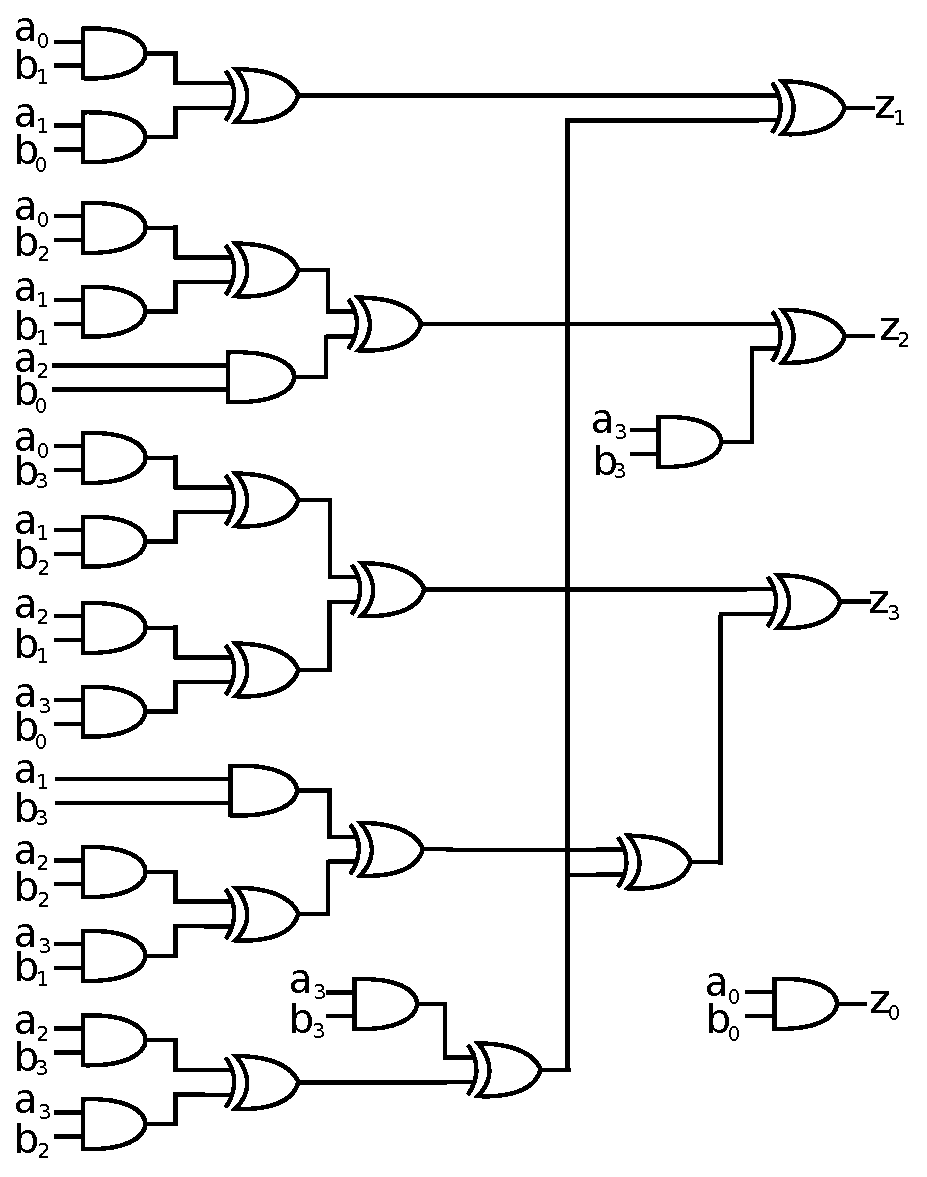
\includegraphics[scale=0.50]{figures/mul4bit.eps}
	\end{center}
	\caption{Mastrovito multiplier over $\mathbb{F}_{2^4}$.}
	\label{fig:mas4}
\end{figure}

Its corresponding composite field design with decomposition $\mathbb{F}_{(2^2)^{2}}$ is shown in Figure \ref{fig:mas22}.
Each block in Fig.\ref{fig:mas22} represents a $2$-bit operation internally, where 
$\times$ represents an $m$-bit multiplier and $+$ represents an $m$-bit adder. 

\begin{sidewaysfigure}
%\begin{figure}[h]
\centerline{
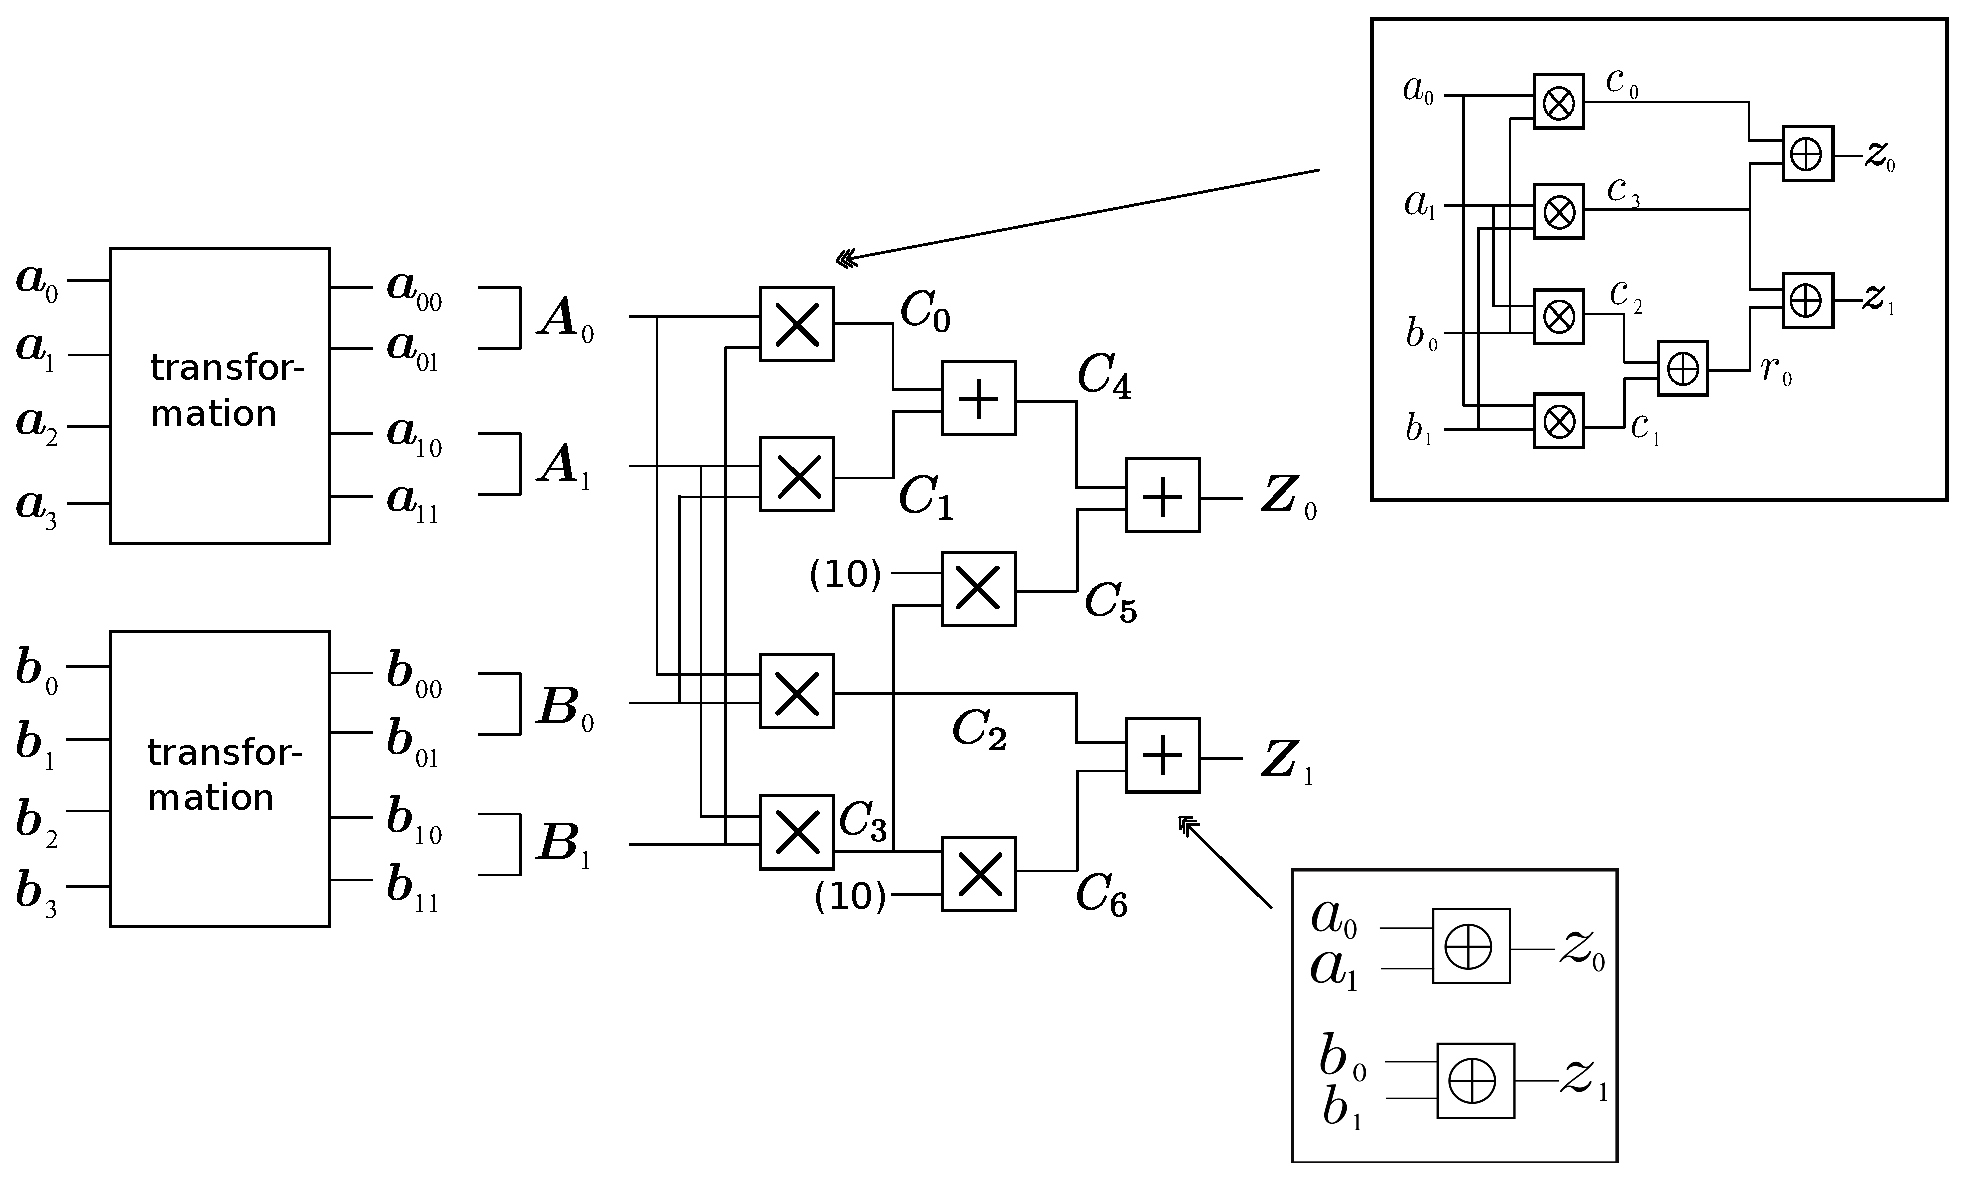
\includegraphics[scale=0.50]{./figures/cfmultiplier.eps}
}
\caption{Mastrovito multiplier over $\mathbb{F}_{(2^2)^2}$}
\label{fig:mas22}
%\end{figure}
\end{sidewaysfigure} 

%%%%%%%%%%%%%%%%%%%%%%%%%%%%%%%%%%%%%%%%%%%%%%
%%%%%%%%%%%%%%%%%%%%%%%%%%%%%%%%%%%%%%%%%%%%%%
%%%%%%%%%%%%%%%%%%%%%%%%%%%%%%%%%%%%%%%%%%%%%%
\section{Problem Formulation and Hierarchy Verification}
\label{sec:setup}

Let us again take the multiplier verification problem as example. 
The {\it specification} $S = A \cdot B \pmod{ P(x)}$ is already given in polynomial form (word level).
The {\it implementation} is available at two different abstraction 
levels: one at the bit-level (ground field $\mathbb{F}_{2^m}$ adders and
multipliers) and one at the higher-level at $\mathbb{F}_{(2^m)^n}$. 
Using this information, we derive constraints (polynomials) $Z$ corresponding to the circuit. 
Our verification problem is to prove/disprove that for all values of the inputs 
$A =\{a_0, \dots a_{k-1}\}, ~B=\{b_0, \dots b_{k-1}\}$, 
the circuit implementation $Z$ correctly computes the multiplication $S$.

As we can notice from Figure \ref{fig:mas22}, the entire composite field circuit is constructed
on lower level building-blocks (adders and multipliers).
Therefore, we have two verification objectives: low level circuits and
higher-level interconnection of the lower-level blocks.

{\bf Verification of low level circuits over $\mathbb{F}_{2^m}$:}

Low level building-blocks consist of adders and multipliers over $\mathbb{F}_{2^m}$.
These circuits are implemented at gate-level and are nothing special 
as the regular finite field circuits we verified before. 
Therefore, we can simply employ the same methods described in Chapter \ref{ch:date}
to formulate the verification test as membership testing of 
the property polynomial ($S+Z=0$). 
When the correctness of low level circuits is certified, we can conduct the
high level verification over $\mathbb{F}_{(2^m)^n}$.

{\bf Verification of higher-level interconnection over $\mathbb{F}_{(2^m)^n}$:}
The difficulty of verifying the composite field circuits 
lies in the verification of high level interconnection of low level building-blocks.
Specifically, due to the presence of hierarchy of composite field circuits, 
the constraints derived from the high level interconnection contain
both gate-level and word-level abstractions. For example, in Figure \ref{fig:mas22},
the circuit hierarchy can be described as follows:
\begin{eqnarray}\label{eqn:compf}
	a_{00}=a_0+a_3 \nonumber  \\
	a_{01}=a_2+a_3 \nonumber  \\
	a_{10}=a_1+a_3  \nonumber  \\
	a_{11}=a_2 \nonumber  \\
	A_0=a_{00}+a_{01} \cdot \alpha ^5 	\nonumber  \\
	A_1=a_{10}+a_{11} \cdot \alpha ^5   \nonumber  \\
	b_{00}=b_0+b_3		\nonumber  \\
	b_{01}=b_2+b_3		\nonumber  \\
	b_{10}=b_1+b_3		\nonumber  \\
	b_{11}=b_2			\nonumber  \\
	B_0=b_{00}+b_{01} \cdot \alpha ^5		\nonumber  \\	 
	B_1=b_{10}+b_{11} \cdot \alpha ^5		\nonumber  \\
	C_0 = A_0\cdot B_1		\nonumber  \\
	C_1 = A_1\cdot B_0		\nonumber  \\
	C_2 = A_0\cdot B_0		\nonumber  \\
	C_3 = A_1\cdot B_1		\nonumber  \\
	C_4 = C_0 + C_1			\nonumber  \\
	C_5 = C_3 \cdot \alpha ^5	\nonumber  \\
	C_6 = C_3 \cdot \alpha ^5	\nonumber  \\
	Z_0 = C_{4}+C_{5}			\nonumber  \\
	Z_{1}=C_{2}+C_{6}			\nonumber  \\ 
\end{eqnarray}
where $a_0, \dots, a_3, b_0,\dots,b_3$ are variables in $\mathbb{F}_{2}$ (bits) while 
$A_0,A_1,B_0,B_1, C_{1},\dots, C_{6}$, $Z_{0}$, $Z_{1}$ are variables in $\mathbb{F}_{2^2}$ (words).
Therefore bit-level variables and word-level variables co-exist in the design.
As far as we know, there are no techniques that can verify design with different levels of abstraction.
This is mainly because BDD/SAT/AIG based approaches can only handle bit-level problems. 
SMT solvers, on the other hand, have no advantages to solve problems at bit-level. 
Besides, SMT solvers formulate every problem over rings instead of finite fields. 
Take Eqnations \ref{eqn:compf} for example, $C_0 = A_0\cdot B_1$ represents a $2$-bit finite field multiplication.
In SMT,  $C_0 = A_0\cdot B_1$ represents a $2$-bit integer multiplication. As we know, the multiplication over rings and over finite fields differs significantly.
 
Fortunately, due to the fact that both bits and words information can be formulated as polynomials,
this verification problem is algebraic in nature and therefore 
can be easily formulated as a system of polynomials and solved by ideal membership testing,
which is described in Algorithm \ref{alg:overall}.

\begin{Example}
		
	Our high-level verification problem is illustrated in Table \ref{tab:masvercf}. 
	Let $F$ denote all the polynomials representing {\it implementation}, {\it specification} and {\it vanishing polynomials}.
	Let $F_0$ denote the vanishing polynomials for primary inputs.
	After all the polynomials in $\{F\}$ are available, 
	we just need to check whether $S+Z$ is a member of the ideal $\langle F,F_0\rangle$.
	
	\begin{table}[t]
	\begin{center}
	\caption{Verification Setup over $\mathbb{F}_{(2^2)^2}$}\label{tab:masvercf}
	\begin{tabular}{|c | c|c|}
	\hline
	{\it implementation} & {\it specification} 	&  {\it vanishing polynomials}\\
	\hline
	$a_{00}+a_0+a_3$ & $A+a_0+a_1\cdot \alpha+a_2\cdot \alpha^2+a_3\cdot \alpha^3$   &$a_0^{2}-a_0$		\\
	$a_{01}+a_2+a_3$ & $B+b_0+b_1\cdot \alpha+b_2\cdot \alpha^2+b_3\cdot \alpha^3$ 	&$a_1^{2}-a_1$			\\
	$a_{10}+a_1+a_3$ &  $S+A\times B$ &$a_2^{2}-a_2$	\\
	$a_{11}+a_2$ &  &$a_3^{2}-a_3$	\\ 
	$A_0+a_{00}+a_{01} \cdot x^5$ & 	&$b_0^{2}-b_0$	\\ 
	$A_1+a_{10}+a_{11} \cdot x^5$ & 	&$b_1^{2}-b_1$\\
	$b_{00}+b_0+b_3$ & &$b_2^{2}-b_2$\\
	$b_{01}+b_2+b_3$ & &$b_3^{2}-b_3$\\
	$b_{10}+b_1+b_3$ & &\\
	$b_{11}+b_2$ & &\\
	$B_0+b_{00}+b_{01} \cdot x^5$ & &\\ 
	$B_1+b_{10}+b_{11} \cdot x^5$ & &\\
	$C_0 + A_0\cdot B_0$    &    &\\
	$C_1 + A_1\cdot B_0$		  &    \\
	$s_2 + A_1\cdot B_1$    &  &\\
	$C_3 + A_1\cdot B_1$		&  &\\
	$C_4 + C_0 + C_1$			& & \\
	$C_5 + C_3 \cdot \alpha ^5$	&  &\\
	$C_6 + C_3 \cdot \alpha ^5$	&  &\\
	$Z_0 + C_{4}+C_{5}$			& & \\
	$Z_{1}+C_{2}+C_{6}$			&  &\\ 
	$Z+Z_{0}+Z_{1}\cdot \alpha $ & &\\ 
	\hline
	\multicolumn{3}{|c|}{Property: $\mathbf{Z+S}$} \\
	\hline
	\end{tabular}
	\end{center}
	\end{table}

\end{Example}

\section{Experimental Results}\label{sec:experiment}

With the approach presented above, we have conducted experiments to
hierarchically verify Mastrovito multiplier implementations $M$
against the specification $S = A\cdot B \pmod{ P(x)}$. Our
verification setup is shown of Table \ref{tab:masvercf}. The implementation
is given as a circuit over $\mathbb{F}_{(2^m)^n}$. With the given hierarchy
information, we construct the polynomials representing high level
designs $M_H$ over $\mathbb{F}_{(2^m)^n}$ and low level designs $M_L$
over $\mathbb{F}_{2^m}$ separately. 

For high level designs $M_H$, the specification polynomials $S = A \cdot B \pmod{ P(x)}$ is used.
In contrast, for low level designs $M_L$ over $\mathbb{F}_{2^m}$, the specification
polynomials $S_L  = A_{m} \cdot B_{m} \pmod{ Q(x)}$ is used, of which,
$A_{m},B_{m}$ represents the $m$-bit inputs for low level building-block circuits;
$Q(x)$ is the primitive polynomial of $\mathbb{F}_{2^m}$.
Then vanishing polynomials ${a_0^2-a_0,\dots,a_{k-1}^2-a_{k-1}, b_0^2-b_0,b_{k-1}^2-b_{k-1}}$ 
are then appended to $M_H$ and $M_L$ at different levels of design.
We use {\sc singular} \cite{DGPS} to conduct polynomial reduction. 
When the circuits are correctly designed, we do observe that reduction result is $0$, 
proving the equivalence. 

Our experiments are conducted on a desktop with $2.40$GHz CPU and $8$GB
memory running $64$-bit Linux. The time-out limit is set as $24$ hours. 

The verification of low level circuits is the same as the one shown in Table \ref{tab:ourmas}. 
The number of low level design units is shown in Table \ref{tbl:stats}. Note
that this number is determined by $n$, which means $\mathbb{F}_{(2^{m_1})^n}$
and $\mathbb{F}_{(2^{m_2})^n}$ have the same number of low level design units,
even if $m_1 \neq m_2$.

Since high level verification cannot be solved by any other technique, we only show the results of our approach.
Table \ref{tbl:modvsword} shows the runtime of high level designs verification over $\mathbb{F}_{(2^m)^n}$ 
for varying word-size $k=m\cdot n$. As shown in Table \ref{tbl:modvsword}, with our approach, 
we are able to prove the correctness of finite field circuits for up to $1024$-bit 
with decomposition $\mathbb{F}_{(2^{32})^{32}}$.

\begin{sidewaystable} 
%\begin{table}[h!]
\begin{center}
\caption{Verification of Mastrovito multiplier over $\mathbb{F}_{(2^m)^n}$ Using Proposed Approach. All times are given in seconds.}
\label{tbl:modvsword}
\begin{tabular}{||c|c|c||c|c|c||c|c|c||c|c|c||c|c|c||c|c|c||} 
\hline
\multicolumn{3}{||c||}{32}&\multicolumn{3}{c||}{64} &
\multicolumn{3}{c||}{128}&\multicolumn{3}{c||}{256} &
\multicolumn{3}{c||}{512}&\multicolumn{3}{c||}{1024}     \\
\hline
$m$& $n$ & time& $m$& $n$ & time& $m$& $n$ & time& $m$& $n$ & time& $m$& $n$ & time& $m$& $n$ & time \\
\hline
$2$  & $16$ & $7.55$ & $2$ & $32$ &$879.83$& $2$& $64$ & $\ast$& $2$ & $128$ & $\ast$ & $2$&$256$&$\ast$ & $2$&$512$&$\ast$\\
\hline
$4$  & $8$  & $0.12$ & $4$ & $16$ & $10.81$& $4$& $32$&$1619.51$& $4$ & $64$  & $\ast$ & $4$&$128$&$\ast$ & $4$&$256$&$\ast$\\
\hline
$8$  & $4$  & $0.01$ & $8$ & $8$  & $0.46$ & $8$& $16$ &$35.04$& $8$ & $32$  & $2664.56$ & $8$&$64$ &$\ast$ & $8$&$128$&$\ast$\\
\hline
$16$ & $2$  & $0.01$ & $16$& $4$  & $0.15$ &$16$& $8$  & $3.25$&$16$ & $16$  &$147.84$&$16$&$32$ &$11510$ & $16$&$64$&$\ast$\\
\hline
 -   & -    & -      & $32$& $2$  & $0.11$ &$32$& $4$  & $2.14$&$32$ & $8$   & $37.71$&$32$&$16$ &$1166.10$&$32$ &$32$ & $75336$  \\
\hline
\end{tabular}
\end{center}

\begin{center}
\caption{Statistics of Designs over $\mathbb{F}_{2^m}$}
\label{tbl:stats}
\begin{tabular}{|c|c|c|c|c|c|c|c|} 
\hline
$n$ & 2 & 4 & 8 & 16 & 32 \\
\hline
\#Multipliers  & $6$ & $36$ & $168$ & $720$ & $2976$ \\
\hline
\#Adders       & $3$ & $27$ & $147$ & $675$ & $2883$  \\
\hline
\end{tabular}
\end{center}
\end{sidewaystable}

\section{Conclusions}
This chapter has targeted the implementation verification of
hierarchically designed composite finite field circuits. 
Decomposing the finite field $\mathbb{F}_{2^k}$ as $\mathbb{F}_{(2^m)^n}$ 
introduces a hierarchical abstraction. Our approach requires that
this hierarchy information be made available. Then, we formulate the
verification problem using the polynomial reduction
as a ideal membership testing at different levels of abstraction.
First we verify low-level adders and
multipliers at $\mathbb{F}_{2^m}$, and then verify the high-level
interconnections between these blocks at $\mathbb{F}_{(2^m)^n}$. Using our
approach, we can verify the correctness of up to 1024-bit multipliers
where other contemporary techniques are not capable of verifying such circuits.
This work was presented in \cite{lv:hldvt2011}.

\chapter{Conclusions and Future Work}\label{ch:concl}
{\ls{1.65}{


This dissertation presents approaches to performing equivalence checking for arithmetic circuits over finite fields 
$\mathbb{F}_{2^k}$. In particular, we target two specific problems: i) verifying the correctness of a custom-designed
arithmetic circuit implementation against a given word-level polynomial specification over ${\mathbb{F}_{2^k}}$; 
and ii) gate-level equivalence checking of two structurally dissimilar arithmetic circuits. 
We propose polynomial abstractions over finite fields to model and represent the circuit constraints. 
Subsequently, decision procedures based on modern computer algebra techniques --
notably Gr\"obner bases related theory and technology -- are
engineered to solve the verification problem efficiently. 

\section{Computer Algebra Based Approaches for Equivalence Checking of Arithmetic Circuit over ${\mathbb{F}_{2^k}}$}

The arithmetic circuit is modeled as a polynomial system in the ring ${\mathbb{F}}_{2^k}[x_1,x_2,\cdots$, $x_d]$, and computer-algebra and
algebraic-geometry based results (Hilbert's Nullstellensatz) over finite fields are exploited for verification. Two formulations are
presented to address the implementation verification and the equivalence checking problems.

Using the results of Strong Nullstellensatz over finite fields, 
the first verification problem is formulated as an ideal membership testing. 
For this ideal membership test, it is required to compute a Gr\"obner basis. 
The Gr\"obner basis computation is known to have double-exponential worst-case complexity in the input data,
which makes this approach impractical. 
Therefore, straight-forward use of Gr\"obner basis engines for verification is
infeasible for large circuits. To overcome this complexity, 
we analyze the given circuit topology to get more theoretical insights
into the polynomial ideals corresponding to the circuit constraints. 
Based on this circuit information,  we derive efficient
term orderings to represent the polynomials. Subsequently, using
the theory of Gr\"obner bases over finite fields, we prove that our
term orderings render the set of polynomials itself a Gr\"obner basis
-- thus obviating the need for Buchberger's algorithm. 
To fulfill our verification purpose, we simply conduct a polynomial reduction to test whether
the equality property is a member of the ideal representing the circuit constraints.


The equivalence checking for two structurally dissimilar arithmetic circuits is still a challenge for contemporary techniques.
By utilizing computer algebra theory, we formulate this problem as a weak Nullstellensatz proof using Gr\"obner bases computation. 
Once again, this would require the computation of a reduced Gr\"obner basis, which is expensive for large circuits. 
To overcome this complexity, we want to exploit our circuit-based term ordering for polynomial representation. 
Unfortunately, unlike in the previous case, the set of polynomials corresponding to this verification instance does 
not constitute a Gr\"obner basis. Instead of computing a Gr\"obner basis for the the whole circuit, 
we identify a minimal number of S-polynomial computations that are sufficient to prove equivalence or 
to detect bugs for the whole circuit.

The verification of composite field circuits is a successful application of our computer algebra based approaches.
To construct a composite field circuit over $\mathbb{F}_{(2^m)^n}$, the finite field $\mathbb{F}_{2^k}$ is 
decomposed as $\mathbb{F}_{(2^m)^n}$, for a $k = m\cdot n$, 
and the arithmetic operations are then performed over $\mathbb{F}_{(2^m)^n}$. 
The decomposition introduces a hierarchy (modularity) in the design by lifting the ground field from $\mathbb{F}_2$
(bits) to $\mathbb{F}_{2^m}$ (words).
We formulate the verification problem as an (radical) ideal membership test at different abstraction levels.
By combining the circuit hierarchy information,  
we first verify the correctness of lower-level building-blocks (adders and 	multipliers) over the ground field $\mathbb{F}_{2^m}$; 
then verify the overall arithmetic at the higher-level over the extension field $\mathbb{F}_{(2^m)^n}$. 		

\section{Future Work}
The approaches and theories presented in this dissertation can be further extended to enhance 
the efficiency of equivalence checking of arithmetic circuits. Some future research directions are proposed here.


\subsection{Speeding up Verification using a Graphics Processing Unit}
As shown in Figure \ref{fig:2bitadder}, the equivalence of ``CIRCUIT1" and ``CIRCUIT2" 
is formulated as a single miter at word-level. However, since the circuits have multiple outputs ($k$),
we can create $k$ miters for each output bit.
In such cases, we will have to compute $Spoly(f_m,f_o) \stackrel{F,F_0}{\longrightarrow}_+ r$ 
for each of the $k$ outputs, and check if $r = 1$ in each case. 
These are going to be $n$ independent computations.
In that regard, they will immensely benefit from parallelization. 

It is desirable to implement this technique on a hardware accelerator -
particularly on a NVIDIA Graphics Processing Unit (GPU). In the
Electronic Design Automation (EDA) community, there has been a lot of
interest in exploiting GPU computing to improve synthesis and
verification algorithms. Significant speed-ups have
been observed in GPU implementation of circuit simulation algorithms
(see for example \cite{PengLi:GPU}). It is needed to further study how to
efficiently implement our circuit verification problem using
independent $S$-polynomial reductions on a general purpose GPU. 

\subsection{Extraction of Circuit Abstraction}

Suppose that we are given a circuit that implements a polynomial
function over $\mathbb{F}_{2^{k}} \rightarrow \mathbb{F}_{2^{k}}$, 
but we do not know what function does it implement. 
Can we identify a polynomial representation of this
function: $f(X, Y)$ where $X$ represents the input bit-vector and $Y$
the output? This problem is one of hierarchy abstraction and is used
in component matching and resource allocation in high-level synthesis. 

To explain this idea, let us re-visit the example of
Figure \ref{fig:2bitmul}, a 2-bit multiplier. It implements a polynomial
function $Z = A * B; ~Z, A, B  \in {\mathbb{F}}_{2^2}$. Here $A= a_0 +
a_1\alpha, B = b_0 + b_1 \alpha, Z = z_0 + z_1\alpha$. Let us
represent a polynomial for each gate in the circuit. We will impose
the following term order: {\bf lex term order} with ``circuit
Variables'' $>$ ``Inputs, A, B'' $>$ ``Output Z''. That is, we use lex
term order with $c_0 > c_1 >  c_2 >  c_3 >  r_0 > a_0 > 
a_1 > b_0 > b_1 > z_0 > z_1 > A > B > Z$. If we use this order to compute a Gr\"obner basis of the circuit
polynomials, then we obtain the following polynomials: 
\begin{eqnarray}
f_1: z_0+z_1\alpha +Z  \nonumber \\
f_2: b_0+b_1\alpha +B  \nonumber \\
f_3: a_0+a_1\alpha +A \nonumber \\
f_4: c_3+r_0+z_1  \nonumber \\
f_5: c_1+c_2+r_0  \nonumber \\
f_6: c_0+c_3+z_0  \nonumber \\
f_7:  A\cdot B+Z 		 \nonumber \\
f_8: a_1\cdot b_1+a_1\cdot B+b_1\cdot A+z_1  \nonumber \\
f_9: r_0+a_1\cdot b_1+z_1 		 \nonumber \\
f_{10}: c_2+a_1\cdot b_0  \nonumber 
\end{eqnarray}
Notice that the polynomial $f_7: A*B + Z$ is indeed the polynomial representation of the
function implemented by the circuit. And we were able to ``extract''
the polynomial representation using Gr\"obner basis. 

Polynomial interpolation techniques for this problem were studied
in  \cite{demicheli:iccad_98} \cite{demicheli:dac_99}. Further research should be conducted to  
investigate if we can use Gr\"obner basis techniques to efficiently
interpolate a polynomial representation from a circuit.


\subsection{Simulation Based Verification of Circuits}
 
In our group's previous work \cite{shekhar:tvlsi} \cite{shekhar:fmcad06}, we
show that given two polynomial functions $f, g$ over $\mathbb{Z}_{2^k}$,  exhaustive
simulation is not always necessary to prove their equivalence. We
identified an integer $\lambda$ such that functions (polynomials) $f,g$ 
need to be evaluated only for $\lambda$ inputs vectors: $\{V_1,
\dots, V_{\lambda}\}$. If $f = g$ for these $\lambda$ vectors, then $f= g$ 
over the entire design space. If $f \neq g$, then we guarantee to
catch the bug within these $\lambda$ vectors. In practice, $\lambda <<2^k$. 

Unfortunately, this result did not find much practical application as
it required that $f, g$ be polynomial functions. Not every function
(circuit) $f: \mathbb{Z}_{2^k} \rightarrow \mathbb{Z}_{2^k}$ is a polynomial
function. Instead of modeling a $k$-input/output circuit as a function
from $f: \mathbb{Z}_{2^k} \rightarrow \mathbb{Z}_{2^k}$, 
We conjecture the model can be viewed as a polynomial function over finite fields 
$f: \mathbb{F}_{2^k} \rightarrow \mathbb{F}_{2^k}$. Though this way, 
we can then prove equivalence of two polyfunctions $f, g: \mathbb{F}_{2^k} \rightarrow \mathbb{F}_{2^k}$
without resorting to exhaustive simulation. 
It is promising to solve the same problem as in \cite{shekhar:tvlsi} \cite{shekhar:fmcad06}, 
but now over a different domain: $\mathbb{F}_{2^k}$. 

%\newpage

%%%%%%%%%%%%%%%%%%%% The bibliography %%%%%%%%%%%%%%%%%%%%%%%%%%%%

\bibliographystyle{ieee}
\bibliography{logic}
\end{document}

%%%%%%%%%%%%%%%%%%%%%%%%%%%  End of IEEEsample.tex  %%%%%%%%%%%%%%%%%%%%%%%%%%%
